%% Copyright (c) 2002, 2010 Sam Williams
%% Copyright (c) 2010 Richard M. Stallman
%% Permission is granted to copy, distribute and/or modify this
%% document under the terms of the GNU Free Documentation License,
%% Version 1.3 or any later version published by the Free Software
%% Foundation; with no Invariant Sections, no Front-Cover Texts, and
%% no Back-Cover Texts. A copy of the license is included in the
%% file called ``gfdl.tex''.

\documentclass[10pt]{book}
\usepackage{url}
\usepackage[Lenny]{fncychap}
\clubpenalty=10000
\widowpenalty=10000

\usepackage{polyglossia}
\setmainlanguage{russian}
\setotherlanguage{english}

\usepackage{fontspec}
\setmainfont{Liberation Serif}
\newfontfamily{\cyrillicfonttt}{Liberation Mono}
\setsansfont{Liberation Sans}
\setmonofont{Liberation Mono}

\usepackage{csquotes}

%% PDF setup
\usepackage{hyperref}
\hypersetup{colorlinks=true, 
           citecolor=blue,
           filecolor=blue,
           linkcolor=blue,
           urlcolor=blue,
           bookmarksopen=true,
           pdftitle=Ричард Столлман и революция свободного программного обеспечения,
           pdfauthor=Ричард Столлман и Сэм Вильямс,
           pdftex}

%% Index
\usepackage{makeidx}
\makeindex

%% Endnotes
\usepackage{endnotes}
\renewcommand\notesname {Примечания}

%% Photos
\usepackage{graphicx}
\usepackage[labelformat=empty,font={small,it}, width=3.75in]{caption}

%% Paper size
\usepackage{geometry}
\geometry{papersize={6in,9in}}

\setcounter{errorcontextlines}{10}

\begin{document}
\title{Ричард Столлман и революция свободного программного обеспечения}
\author{Сэм Вильямс \\ Второе издание с правками от Ричарда Мэттью Столлмана}
\date{}

\maketitle
\thispagestyle{empty}
\frontmatter
\noindent This is \textit{Free as in Freedom 2.0: Richard Stallman and
  the Free Software Revolution}, a revision of \textit{Free as in
  Freedom: Richard Stallman's Crusade for Free Software}.

\bigskip

\noindent Copyright \copyright{} 2002, 2010 Sam Williams\\
Copyright \copyright{} 2010 Richard M. Stallman\\
Permission is granted to copy, distribute and/or modify
this document under the terms of the GNU Free Documentation License,
Version 1.3 or any later version published by the Free Software
Foundation; with no Invariant Sections, no Front-Cover Texts, and no
Back-Cover Texts. A copy of the license is included in the section
entitled ``GNU Free Documentation License.''

\bigskip

\noindent Published by the Free Software Foundation\\
51 Franklin St., Fifth Floor\\
Boston, MA 02110-1335\\
USA\\
ISBN: 9780983159216\\

\bigskip

\noindent The cover photograph of Richard Stallman is by Peter Hinely. The PDP-10 photograph in Chapter 7 is by Rodney Brooks. The photograph of St. IGNUcius in Chapter 8 is by Stian Eikeland. 

\thispagestyle{empty}
\tableofcontents
%% Copyright (c) 2002, 2010 Sam Williams
%% Copyright (c) 2010 Richard M. Stallman
%% Permission is granted to copy, distribute and/or modify this
%% document under the terms of the GNU Free Documentation License,
%% Version 1.3 or any later version published by the Free Software
%% Foundation; with no Invariant Sections, no Front-Cover Texts, and
%% no Back-Cover Texts. A copy of the license is included in the
%% file called ``gfdl.tex''.


\chapter[Foreword by Richard M. Stallman]{Foreword\\by Richard M. Stallman}

I have aimed to make this edition combine the advantages of my
knowledge and Williams' interviews and outside viewpoint.  The reader
can judge to what extent I have achieved this.

I read the published text of the English edition for the first time in
2009 when I was asked to assist in making a French translation of \textit{Free
as in Freedom}.  It called for more than small changes.

Many facts needed correction, but deeper changes were also needed.
Williams, a non-programmer, blurred fundamental technical and legal
distinctions, such as that between modifying an existing program's
code, on the one hand, and implementing some of its ideas in a new
program, on the other.  Thus, the first edition said that both Gosmacs
and GNU Emacs were developed by modifying the original PDP-10 Emacs,
which in fact neither one was.  Likewise, it mistakenly
described Linux as a ``version of Minix.''  SCO later made the same
false claim in its infamous lawsuit against IBM, and both Torvalds and
Tanenbaum rebutted it.

The first edition overdramatized many events by projecting spurious
emotions into them.  For instance, it said that I ``all but shunned''
Linux in 1992, and then made a ``a dramatic about-face'' by deciding in
1993 to sponsor Debian GNU/Linux.  Both my interest in 1993 and my
lack of interest in 1992 were pragmatic means to pursue the same end:
to complete the GNU system.  The launch of the GNU Hurd kernel in 1990
was also a pragmatic move directed at that same end.

For all these reasons, many statements in the original edition were
mistaken or incoherent.  It was necessary to correct them, but not
straightforward to do so with integrity short of a total rewrite,
which was undesirable for other reasons.  Using explicit notes for the
corrections was suggested, but in most chapters the amount of change
made explicit notes prohibitive.  Some errors were too pervasive or
too ingrained to be corrected by notes.  Inline or footnotes for the
rest would have overwhelmed the text in some places and made the text
hard to read; footnotes would have been skipped by readers tired of
looking down for them.  I have therefore made corrections directly in
the text.

However, I have not tried to check all the facts and quotations that
are outside my knowledge; most of those I have simply carried forward
on Williams' authority.

Williams' version contained many quotations that are critical of me.  I
have preserved all these, adding rebuttals when appropriate.  I have
not deleted any quotation, except in \autoref{chapter:open source} where I have deleted
some that were about open source and did not pertain to my life or
work.  Likewise I have preserved (and sometimes commented on) most of
Williams' own interpretations that criticized me, when they did not
represent misunderstanding of facts or technology, but I have freely
corrected inaccurate assertions about my work and my thoughts and
feelings.  I have preserved his personal impressions when presented as
such, and ``I'' in the text of this edition always refers to Williams
except in notes labeled ``RMS:''.

In this edition, the complete system that combines GNU and Linux is
always ``GNU/Linux,'' and ``Linux'' by itself always refers to Torvalds'
kernel, except in quotations where the other usage is marked with
``[\textit{sic}]''.  See \url{http://www.gnu.org/gnu/gnu-linux-faq.html} for more
explanation of why it is erroneous and unfair to call the whole system
``Linux.''

I would like to thank John Sullivan for his many useful criticisms and
suggestions.

%% Copyright (c) 2002, 2010 Sam Williams
%% Copyright (c) 2010 Richard M. Stallman
%% Permission is granted to copy, distribute and/or modify this
%% document under the terms of the GNU Free Documentation License,
%% Version 1.3 or any later version published by the Free Software
%% Foundation; with no Invariant Sections, no Front-Cover Texts, and
%% no Back-Cover Texts. A copy of the license is included in the
%% file called ``gfdl.tex''.

\chapter{Предисловие от Сэма Вильямса}

Этим летом исполнилось 10 лет той переписке по электронной почте,
что дала начало книге \enquote{Крестовый
поход Ричарда Столлмана за свободное программное обеспечение} и её
доработанной версии: \enquote{Ричард Столлман и революция свободного
программного обеспечения}, которую вы держите в руках.

Не стоит и говорить, что за эти 10 лет многое изменилось в этом мире.

Книгу эту я задумывал в эпоху триумфа Америки, и её суть была совсем
не созвучна победному маршу технокапиталистической модели.
Герой этой книги подобно Иеремии пытается обратить внимание
разработчиков ПО не на экономический потенциал компьютерных
программ, а на этические ценности и обязательства. Он старается донести
до людей, что уход от интеллектуальной и культурной свободы к
выгодному собственничеству дорого обойдётся в будущем.

Теперь же настроения в обществе прямо противоположны -- умы
захватили сомнения в Системе, и потому интересно посмотреть,
какие идеи не потеряли актуальности за эти 10 лет.

Я уже не так пристально слежу за состоянием дел в индустрии ПО,
как раньше, но одно очевидно даже для меня: люди легко отказываются
от личных прав и свобод ради того, чтобы пользоваться всякими
классными и удобными технологиями, и чтобы просто быть модными.

В этом я убедился ещё несколько лет назад, когда случилось то, что
можно назвать \enquote{iPod-эффектом}: музыкальная индустрия и простые
слушатели стали сходить с ума по плееру Apple iPod и сервису iTunes,
при их огромном количестве ограничений. Позже эта история повторилась
с планшетом Apple iPad и электронной книгой Amazon Kindle. Мода на
все эти гаджеты привела к тектоническим сдвигам в индустрии.

Ричарду Столлману, кстати, не понравилось, что я в предисловии как будто
рекламирую несвободные устройства, так что для баланса я скажу
вам про парочку интернет-сайтов, где подробно разбирают недостатки
этих и других продуктов:  \url{DefectiveByDesign.org} и \url{BadVista.org}.

Не имеет значения, о каком именно бренде идёт речь. Люди привыкли
ассоциировать бренды с неким качеством, и этот стереотип побороть
очень трудно. Даже несмотря на многие неудачи и провалы корпораций,
в том числе и экономические.

Десяток лет назад было обычным делом поучаствовать в конференции,
где старожилы программирования вроде Ричарда Столлмана говорили
об альтернативном будущем. И теперь я убедился, куда завела нас,
тогдашних новичков в журналистике, гордость владения новейшими
инструментами вроде Microsoft Word, PowerPoint, Internet Explorer. Все
эти продукты были удобными, заманчивыми пристанищами для тех, кто
работал на компьютере, и благодаря популярности они разрослись в
огромный город программной экосистемы персональных компьютеров.

Город этот похож на антиутопическую диктатуру, где движение, развитие,
жизнь строго регламентированы и возможны лишь в указанных сверху
местах. Неудивительно, что хакеры не прекращают критически ворчать
в адрес структурных недостатков Windows, диктаторского надзора Apple
над их магазином приложений, постоянно меняющегося определения \enquote{зла}
у Google. С каждым годом всё сильнее разрастается \enquote{цифровая реальность},
где пользователи служат гоббсовой корпократии. Наверное, потому что
свободное ПО подкидывает изрядное количество проблем, которые
заставляют пользователей скрежетать зубами.

Как бы то ни было, развитие софта с его бесконечным бегом на шаг
впереди пользовательских вкусов и потребностей всё сильнее толкает
разработчиков к наживе. Нельзя сказать, что хакерская этика умерла или
даже сильно ослабела. Я просто думаю, что вряд ли программист,
который добивается для заказчика высочайших показателей, будет
сидеть в своём Порше и размышлять о том, как развивались бы его
программы без корпоративных кандалов.

Впрочем, десятки и сотни миллионов человек пользуются многими
свободными программами, а какая-то их часть использует только
свободное ПО. Однако понятия вроде \enquote{программное обеспечение}
или \enquote{компьютер} уходят из потребительского лексикона. Нынешние
мобильные телефоны сравнимы с ноутбуками десятилетней давности,
но многие ли при покупке телефона думают о свободе комплектующих
или операционной системы? Единственное, что интересует большинство
-- приложения, которые можно установить, надёжность работы сети, и
самое важное -- тарифные планы.

Заставить современного потребителя взглянуть на софт и оборудование
не с точки зрения удобства и функциональности, а с точки зрения свободы
-- если не невозможно, то довольно сложно.

И вот на такой пессимистичной ноте можно задаться вопросом: зачем
тогда вообще нужна эта книга и кого она может заинтересовать?

Я могу предложить целых две причины.

Первая причина -- личная. В эпилоге книги рассказывается, что я и
Ричард расстались на не совсем тёплой ноте незадолго до публикации.
Виноват в этом, по большей части, я. Довольно плотно поработав с ним,
чтобы быть уверенным, что моя книга не противоречит ценностям
свободного ПО -- с гордостью, кстати, сообщаю, что это одна из первых
книг, что использует GNU Free Documentation License -- я резко оборвал
сотрудничество, когда настала пора редактирования и Ричард прислал
длиннющий список исправлений.

Хоть я умею виртуозно прятаться за своими принципами вроде
авторской независимости и журналистской объективности, я не стал
ходить к издателю и умолять его о дополнительном времени. Ведь
О'Рейли и так сделал мне огромную уступку -- позволил выбрать GFDL
в качестве лицензии. Наверное, он бы согласился и с огромным потоком
исправлений перед самой публикацией, но я не стал испытывать удачу.

По прошествии нескольких лет у меня появилось ещё одно оправдание
этому шагу: сама лицензия GFDL, которая позволяет любому читателю
редактировать книгу и распространять свой вариант. Как однажды
сказал Эрнест Хемингуэй: \enquote{Первый черновик -- всегда дерьмо}.
Если Столлман и другие хакеры сообщества свободного ПО считали
мою книгу первым черновиком, то что ж -- по крайней мере, я избавил
их от этой неблагодарной работы.

Теперь же я могу только одобрить множество правок Ричарда, чтобы
остаться верным себе. На самом деле, я их даже приветствую. Видя, что
активность Ричарда и не думает снижаться, я надеюсь только, что его
правки включат в себя множество документальных дополнений.

Прежде чем перейти ко второй причине, хочу отметить, что работа над
этой книгой имела приятный побочный эффект -- возобновление нашего
со Столлманом общения по электронной почте. Я снова могу получать
удовольствие от его острого как бритва стиля изложения.

Те, кто когда-либо дискутировал со Столлманом в переписке, найдут
показательным и забавным следующий случай. Рецензенты часто критиковали
главу, где описывается, как мы едем через Кихеи на Мауи (\enquote{Краткое
путешествие по аду хакера}) -- мол, она выбивается из общей канвы
и выглядит неуместной. Я сказал Ричарду, что он может вырезать эту
главу, но заметил, что она даёт неплохое метафорическое описание
его характера и вообще хакерского мышления.

К моему удивлению, Столлман со мной согласился. Его больше заботили
отдельные неточности в тексте. Например, я устами Ричарда выразил, что
ведущий нас местный житель \enquote{специально} ведёт нас такой дорогой,
что придало его поведению ноту злого умысла. К сожалению, я мог
положиться лишь на записи -- довольно ненадёжный источник. Из-за
этого я исказил формулировки Ричарда, сделав их более жёсткими.

Вопросы у Столлмана возникли и к слову \enquote{долбаный}. Опять же, я не
мог обратиться к аудиозаписи диктофона, но сказал Ричарду, что меня
тогда впечатлила его лексика, напомнив мне о его нью-йоркских корнях,
так что я уверен в использованном слове.

На следующий день пришло ответное письмо, которое заставило меня
перечитать предыдущее сообщение. Оказалось, что Столлман спорит
не с самим словом, а с той формой, которую я использовал в книге.

\enquote{Сомневаюсь, что я назвал бы чью-то ошибку \enquote{долбаной}, -- писал
мне Ричард, -- мне несвойственно так выражаться. Я бы скорее сказал:
\enquote{долбанутая ошибка}. Поэтому я думаю, что слова искажены}.

Шах и мат.

Вторая причина существования этой книги и чьего-либо интереса к
ней возвращает нас к началу предисловия -- разница между началом
века и его вторым десятилетием. Буду честен: мои взгляды сильно
поменялись после 11 сентября 2001 года, так что скоро после выхода
первой версии книги я почти совсем перестал следить за Столлманом
и движением за свободное ПО. Хотя основные тенденции и проблемы
индустрии ПО всё-таки достигали моего внимания, основная масса
событий скрылась от меня, подобно подводной части айсберга.

[РМС: Атаки 11 сентября 2001 года почти не упоминаются в книге,
 но я думаю, что стоит дать краткий комментарий на эту тему. Хотя
 многие думают и заявляют, что эти теракты \enquote{изменили всё}, на
 самом деле, они не изменили ничего, в том плане, что во власти
 всё так же сидят негодяи, которые ненавидят наши свободы. Но
 теперь они могут ссылаться на \enquote{террористов} всякий раз, когда
 хотят ввести законы, отбирающие наши права. Подробнее об
 этом можно почитать в политических заметках на моём сайте
 \url{stallman.org}.]

Это весьма плачевно, потому что перед моими глазами тот самый
XXI век, который я считал когда-то светлым будущим. Но сейчас
его уместно назвать веком бега на месте. Я объясню, почему.

Мы находимся в необычной точке исторического развития, где
возможность изменить мир, невзирая на весь цинизм и пессимизм,
действительно доступна каждому. Но в этой доступности каждому
и кроется подвох. Если в прошлом можно было добиться перемен,
завоевав расположение нескольких влиятельных фигур, то теперь
реформатор должен придать нужное направление целому полю
всевозможных идей, настроений и интересов самых разных людей.
То есть, эффективный реформатор должен обладать в наше время
титанической волей и упорством, готовностью десятилетиями
голосить в пустыне, а также массой знаний и творческими талантами,
чтобы создать идеи, способные обыграть Систему в её же игре.

И Ричард Столлман подходит под все эти критерии.

Кто-то может оплакивать насмерть забюрократизированное будущее,
в котором любая проблема требует собраний и заседаний комитетов
и подкомитетов, чтобы только наметить возможные пути её решения.
Я же вижу кое-что другое. Я вижу, как реальность настолько чутко
реагирует на личности и небольшие группы людей, что находится
самозваный актёр, дерзнувший испробовать эту чуткость для того,
чтобы изменить мир.

И если вы один из тех, кто надеется, что XXI век будет намного более
человечным, чем XX век, то -- добро пожаловать в битву. Эпиграф к
первой главе намекает на мою надежду, что эта книга станет эпосом
интернет-эры, построенным вокруг странной героической фигуры.

Так что я хочу закончить это предисловие так же, как закончил
эпилог -- предложением присоединиться к улучшению книги. Текст
лицензии GFDL расскажет вам о ваших правах отредактировать книгу
или даже создать производную версию. Если хотите, можете выслать
свои правки мне или Ричарду. Его контакты вы найдёте на сайте
фонда свободного ПО.

А теперь -- желаю удачи и удовольствия от чтения книги!

\vspace{0.5in}
\noindent Сэм Вильямс\\
\noindent Статен-Айленд, США


\mainmatter
%% Copyright (c) 2002, 2010 Sam Williams
%% Copyright (c) 2010 Richard M. Stallman
%% Permission is granted to copy, distribute and/or modify this
%% document under the terms of the GNU Free Documentation License,
%% Version 1.3 or any later version published by the Free Software
%% Foundation; with no Invariant Sections, no Front-Cover Texts, and
%% no Back-Cover Texts. A copy of the license is included in the
%% file called ``gfdl.tex''.

\chapter{For Want of a Printer}

\begin{quotation}
  \begin{flushright}
    I fear the Greeks. Even when they bring gifts.\\
    -- Virgil, \textit{The Aeneid}
  \end{flushright}
\end{quotation}

The new printer was jammed, again.

Richard M. Stallman, a staff software programmer at the Massachusetts Institute of Technology's Artificial Intelligence Laboratory (AI Lab), discovered the malfunction the hard way. An hour after sending off a 50-page file to the office laser printer, Stallman, 27, broke off a productive work session to retrieve his documents. Upon arrival, he found only four pages in the printer's tray. To make matters even more frustrating, the four pages belonged to another user, meaning that Stallman's print job and the unfinished portion of somebody else's print job were still trapped somewhere within the electrical plumbing of the lab's computer network.

Waiting for machines is an occupational hazard when you're a software programmer, so Stallman took his frustration with a grain of salt. Still, the difference between waiting for a machine and waiting on a machine is a sizable one. It wasn't the first time he'd been forced to stand over the printer, watching pages print out one by one. As a person who spent the bulk of his days and nights improving the efficiency of machines and the software programs that controlled them, Stallman felt a natural urge to open up the machine, look at the guts, and seek out the root of the problem.

Unfortunately, Stallman's skills as a computer programmer did not extend to the mechanical-engineering realm. As freshly printed documents poured out of the machine, Stallman had a chance to reflect on other ways to circumvent the printing jam problem.

How long ago had it been that the staff members at the AI Lab had welcomed the new printer with open arms? Stallman wondered. The machine had been a donation from the Xerox Corporation. A cutting edge prototype, it was a modified version of a fast Xerox photocopier. Only instead of making copies, it relied on software data piped in over a computer network to turn that data into professional-looking documents. Created by engineers at the world-famous Xerox Palo Alto Research Facility, it was, quite simply, an early taste of the desktop-printing revolution that would seize the rest of the computing industry by the end of the decade.

Driven by an instinctual urge to play with the best new equipment, programmers at the AI Lab promptly integrated the new machine into the lab's sophisticated computing infrastructure. The results had been immediately pleasing. Unlike the lab's old printer, the new Xerox machine was fast. Pages came flying out at a rate of one per second, turning a 20-minute print job into a 2-minute print job. The new machine was also more precise. Circles came out looking like circles, not ovals. Straight lines came out looking like straight lines, not low-amplitude sine waves.

It was, for all intents and purposes, a gift too good to refuse.

Once the machine was in use, its flaws began to surface. Chief among the drawbacks was the machine's susceptibility to paper jams. Engineering-minded programmers quickly understood the reason behind the flaw. As a photocopier, the machine generally required the direct oversight of a human operator. Figuring that these human operators would always be on hand to fix a paper jam, if it occurred, Xerox engineers had devoted their time and energies to eliminating other pesky problems. In engineering terms, user diligence was built into the system.

In modifying the machine for printer use, Xerox engineers had changed the user-machine relationship in a subtle but profound way. Instead of making the machine subservient to an individual human operator, they made it subservient to an entire networked population of human operators. Instead of standing directly over the machine, a human user on one end of the network sent his print command through an extended bucket brigade of machines, expecting the desired content to arrive at the targeted destination and in proper form. It wasn't until he finally went to check up on the final output that he realized how little of it had really been printed.

Stallman was hardly the only AI Lab denizen to notice the problem, but he also thought of a remedy. Years before, for the lab's previous printer, Stallman had solved a similar problem by modifying the software program that regulated the printer, on a small PDP-11 machine, as well as the Incompatible Timesharing System that ran on the main PDP-10 computer. Stallman couldn't eliminate paper jams, but he could insert software code that made the PDP-11 check the printer periodically, and report jams back to the PDP-10. Stallman also inserted code on the PDP-10 to notify every user with a waiting print job that the printer was jammed. The notice was simple, something along the lines of ``The printer is jammed, please fix it,'' and because it went out to the people with the most pressing need to fix the problem, chances were that one of them would fix it forthwith.

As fixes go, Stallman's was oblique but elegant. It didn't fix the mechanical side of the problem, but it did the next best thing by closing the information loop between user and machine. Thanks to a few additional lines of software code, AI Lab employees could eliminate the 10 or 15 minutes wasted each week in running back and forth to check on the printer. In programming terms, Stallman's fix took advantage of the amplified intelligence of the overall network.

``If you got that message, you couldn't assume somebody else would fix it,'' says Stallman, recalling the logic. ``You had to go to the printer. A minute or two after the printer got in trouble, the two or three people who got messages arrive to fix the machine. Of those two or three people, one of them, at least, would usually know how to fix the problem.''

Such clever fixes were a trademark of the AI Lab and its indigenous population of programmers. Indeed, the best programmers at the AI Lab disdained the term programmer, preferring the more slangy occupational title of hacker instead. The job title covered a host of activities -- everything from creative mirth making to the improvement of existing software and computer systems. Implicit within the title, however, was the old-fashioned notion of Yankee ingenuity. For a hacker, writing a software program that worked was only the beginning. A hacker would try to display his cleverness (and impress other hackers) by tackling an additional challenge: to make the program particularly fast, small, powerful, elegant, or somehow impressive in a clever way.\endnote{For more on the term ``hacker,'' see \nameref{Appendix A}.}

Companies like Xerox made it a policy to donate their products (and software) to places where hackers typically congregated. If hackers used these products, they might go to work for the company later on.  In the 60s and early 70s, they also sometimes developed programs that were useful for the manufacturer to distribute to other customers.

When Stallman noticed the jamming tendency in the Xerox laser printer, he thought of applying the old fix or ``hack'' to this printer. In the course of looking up the Xerox laser-printer software, however, Stallman made a troubling discovery. The printer didn't have any software, at least nothing Stallman or a fellow programmer could read. Until then, most companies had made it a form of courtesy to publish source-code files--readable text files that documented the individual software commands that told a machine what to do. Xerox, in this instance, had provided software files only in compiled, or binary, form. If programmers looked at the files, all they would see was an endless stream of ones and zeroes -- gibberish.

There are programs, called ``disassemblers,'' to convert the ones and zeroes into low-level machine instructions, but figuring out what those instructions actually ``do'' is a long and hard task, known as ``reverse engineering.''  To reverse engineer this program could have taken more time than five years' worth of jammed printouts.  Stallman wasn't desperate enough for that, so he put the problem aside.

Xerox's unfriendly policy contrasted blatantly with the usual practices of the hacker community.  For instance, to develop the program for the PDP-11 that ran the old printer, and the program for another PDP-11 that handled display terminals, the AI Lab needed a cross-assembler program to build PDP-11 programs on the PDP-10 main computer. The lab's hackers could have written one, but Stallman, a Harvard student, found such a program at Harvard's computer lab. That program was written to run on the same kind of computer, the PDP-10, albeit with a different operating system. Stallman never knew who had written the program, since the source code did not say.  But he brought a copy back to the AI Lab. He then altered the source code to make it run on the AI Lab's Incompatible Timesharing System (ITS). With no muss and little fuss, the AI Lab got the program it needed for its software infrastructure. Stallman even added a few features not found in the original version, making the program more powerful. ``We wound up using it for several years,'' Stallman says.

From the perspective of a 1970s-era programmer, the transaction was the software equivalent of a neighbor stopping by to borrow a power tool or a cup of sugar from a neighbor. The only difference was that in borrowing a copy of the software for the AI Lab, Stallman had done nothing to deprive anyone else of the use of the program. If anything, other hackers gained in the process, because Stallman had introduced additional features that other hackers were welcome to borrow back.  For instance, Stallman recalls a programmer at the private engineering firm, Bolt, Beranek \& Newman, borrowing the program. He made it run on Twenex and added a few additional features, which Stallman eventually reintegrated into the AI Lab's own source-code archive.  The two programmers decided to maintain a common version together, which had the code to run either on ITS or on Twenex at the user's choice.

``A program would develop the way a city develops,'' says Stallman, recalling the software infrastructure of the AI Lab. ``Parts would get replaced and rebuilt. New things would get added on. But you could always look at a certain part and say, `Hmm, by the style, I see this part was written back in the early 60s and this part was written in the mid-1970s.'\hspace{0.01in}''

Through this simple system of intellectual accretion, hackers at the AI Lab and other places built up robust creations. Not every programmer participating in this culture described himself as a hacker, but most shared the sentiments of Richard M. Stallman. If a program or software fix was good enough to solve your problems, it was good enough to solve somebody else's problems. Why not share it out of a simple desire for good karma?

This system of cooperation was being undermined by commercial secrecy and greed, leading to peculiar combinations of secrecy and cooperation.  For instance, computer scientists at UC Berkeley had built up a powerful operating system called BSD, based on the Unix system they had obtained from AT\&T.  Berkeley made BSD available for the cost of copying a tape, but would only give these tapes to schools that could present a \$50,000 source license obtained from AT\&T.  The Berkeley hackers continued to share as much as AT\&T let them, but they had not perceived a conflict between the two practices.

Likewise, Stallman was annoyed that Xerox had not provided the source-code files, but not yet angry.  He never thought of asking Xerox for a copy. ``They had already given us the laser printer,'' Stallman says. ``I could not say they owed us something more.  Besides, I took for granted that the absence of source code reflected an intentional decision, and that asking them to change it would be futile.''

Good news eventually arrived: word had it that a scientist at the computer-science department at Carnegie Mellon University had a copy of the laser printer source code.

The association with Carnegie Mellon did not augur well. In 1979, Brian Reid, a doctoral student there, had shocked the community by refusing to share his text-formatting program, dubbed Scribe.  This text formatter was the first to have mark-up commands oriented towards the desired semantics (such as ``emphasize this word'' or ``this paragraph is a quotation'') rather than low-level formatting details (``put this word in italics'' or ``narrow the margins for this paragraph''). Instead Reid sold Scribe to a Pittsburgh-area software company called Unilogic. His graduate-student career ending, Reid says he simply was looking for a way to unload the program on a set of developers that would take pains to keep it from slipping into the public domain.  (Why one would consider such an outcome particularly undesirable is not clear.) To sweeten the deal, Reid also agreed to insert a set of time-dependent functions -- ``time bombs'' in software-programmer parlance -- that deactivated freely copied versions of the program after a 90-day expiration date. To avoid deactivation, users paid the software company, which then issued a code that defused the internal time-bomb anti-feature.

For Stallman, this was a betrayal of the programmer ethos, pure and simple. Instead of honoring the notion of share-and-share alike, Reid had inserted a way for companies to compel programmers to pay for information access.  But he didn't think deeply about the question, since he didn't use Scribe much.

Unilogic gave the AI Lab a gratis copy to use, but did not remove or mention the time bomb.  It worked, for a while; then one day a user reported that Scribe had stopped working.  System hacker Howard Cannon spent hours debugging the binary until he found the time-bomb and patched it out.  Cannon was incensed, and wasn't shy about telling the other hackers how mad he was that Unilogic had wasted his time with an intentional bug.

Stallman had a Lab-related reason, a few months later, to visit the Carnegie Mellon campus. During that visit, he made a point of looking for the person reported to have the printer software source code.  By good fortune, the man was  in his office.

In true engineer-to-engineer fashion, the conversation was cordial but blunt. After briefly introducing himself as a visitor from MIT, Stallman requested a copy of the laser-printer source code that he wanted to modify. To his chagrin, the researcher refused.

``He told me that he had promised not to give me a copy,'' Stallman says.

Memory is a funny thing. Twenty years after the fact, Stallman's mental history tape is blank in places. Not only does he not remember the motivating reason for the trip or even the time of year during which he took it, he also has no recollection of who was on the other end of the conversation. According to Reid, the person most likely to have fielded Stallman's request is Robert Sproull, a former Xerox PARC researcher and current director of Sun Laboratories, a research division of the computer-technology conglomerate Sun Microsystems. During the 1970s, Sproull had been the primary developer of the laser-printer software in question while at Xerox PARC. Around 1980, Sproull took a faculty research position at Carnegie Mellon where he continued his laser-printer work amid other projects.

When asked directly about the request, however, Sproull draws a blank. ``I can't make a factual comment,'' writes Sproull via email. ``I have absolutely no recollection of the incident.''

``The code that Stallman was asking for was leading-edge, state-of-the-art code that Sproull had written in the year or so before going to Carnegie Mellon,'' recalls Reid.  If so, that might indicate a misunderstanding that occurred, since Stallman wanted the source for the program that MIT had used for quite some time, not some newer version. But the question of which version never arose in the brief conversation.

In talking to audiences, Stallman has made repeated reference to the incident, noting that the man's unwillingness to hand over the source code stemmed from a nondisclosure agreement, a contractual agreement between him and the Xerox Corporation giving the signatory access to the software source code in exchange for a promise of secrecy. Now a standard item of business in the software industry, the nondisclosure agreement, or NDA, was a novel development at the time, a reflection of both the commercial value of the laser printer to Xerox and the information needed to run it. ``Xerox was at the time trying to make a commercial product out of the laser printer,'' recalls Reid. ``They would have been insane to give away the source code.''

For Stallman, however, the NDA was something else entirely. It was a refusal on the part of some CMU researcher to participate in a society that, until then, had encouraged software programmers to regard programs as communal resources. Like a peasant whose centuries-old irrigation ditch had grown suddenly dry, Stallman had followed the ditch to its source only to find a brand-spanking-new hydroelectric dam bearing the Xerox logo.

For Stallman, the realization that Xerox had compelled a fellow programmer to participate in this newfangled system of compelled secrecy took a while to sink in. In the first moment, he could only see the refusal in a personal context. ``I was so angry I couldn't think of a way to express it. So I just turned away and walked out without another word,'' Stallman recalls. ``I might have slammed the door. Who knows? All I remember is wanting to get out of there. I went to his office expecting him to cooperate, so I had not thought about how I would respond if he refused.  When he did, I was stunned speechless as well as disappointed and angry.''

Twenty years after the fact, the anger still lingers, and Stallman presents the event as one that made him confront an ethical issue, though not the only such event on his path. Within the next few months, a series of events would befall both Stallman and the AI Lab hacker community that would make 30 seconds worth of tension in a remote Carnegie Mellon office seem trivial by comparison. Nevertheless, when it comes time to sort out the events that would transform Stallman from a lone hacker, instinctively suspicious of centralized authority, to a crusading activist applying traditional notions of liberty, equality, and fraternity to the world of software development, Stallman singles out the Carnegie Mellon encounter for special attention.

``It was my first encounter with a nondisclosure agreement, and it immediately taught me that nondisclosure agreements have victims,'' says Stallman, firmly. ``In this case I was the victim. [My lab and I] were victims.''

Stallman later explained, ``If he had refused me his cooperation for personal reasons, it would not have raised any larger issue.  I might have considered him a jerk, but no more.  The fact that his refusal was impersonal, that he had promised in advance to be uncooperative, not just to me but to anyone whatsoever, made this a larger issue.''

Although previous events had raised Stallman's ire, he says it wasn't until his Carnegie Mellon encounter that he realized the events were beginning to intrude on a culture he had long considered sacrosanct.  He said, ``I already had an idea that software should be shared, but I wasn't sure how to think about that. My thoughts weren't clear and organized to the point where I could express them in a concise fashion to the rest of the world. After this experience, I started to recognize what the issue was, and how big it was.''

As an elite programmer at one of the world's elite institutions, Stallman had been perfectly willing to ignore the compromises and bargains of his fellow programmers just so long as they didn't interfere with his own work. Until the arrival of the Xerox laser printer, Stallman had been content to look down on the machines and programs other computer users grimly tolerated.

Now that the laser printer had insinuated itself within the AI Lab's network, however, something had changed. The machine worked fine, barring the paper jams, but the ability to modify software according to personal taste or community need had been taken away. From the viewpoint of the software industry, the printer software represented a change in business tactics. Software had become such a valuable asset that companies no longer accepted the need to publicize source code, especially when publication meant giving potential competitors a chance to duplicate something cheaply. From Stallman's viewpoint, the printer was a Trojan Horse. After a decade of failure, software that users could not change and redistribute -- future hackers would use the term ``proprietary'' software -- had gained a foothold inside the AI Lab through the sneakiest of methods. It had come disguised as a gift.

That Xerox had offered some programmers access to additional gifts in exchange for secrecy was also galling, but Stallman takes pains to note that, if presented with such a quid pro quo bargain at a younger age, he just might have taken the Xerox Corporation up on its offer. The anger of the Carnegie Mellon encounter, however, had a firming effect on Stallman's own moral lassitude. Not only did it give him the necessary anger to view such future offers with suspicion, it also forced him to turn the situation around: what if a fellow hacker dropped into Stallman's office someday and it suddenly became Stallman's job to refuse the hacker's request for source code?

``When somebody invited me to betray all my colleagues in that way, I remembered how angry I was when somebody else had done that to me and my whole lab,'' Stallman says. ``So I said, `Thank you very much for offering me this nice software package, but I can't accept it on the conditions that you're asking for, so I'm going to do without it.'\hspace{0.01in}''

It was a lesson Stallman would carry with him through the tumultuous years of the 1980s, a decade during which many of his MIT colleagues would depart the AI Lab and sign nondisclosure agreements of their own. They may have told themselves that this was a necessary evil so they could work on the best projects. For Stallman, however, the NDA called the the moral legitimacy of the project into question.  What good is a technically exciting project if it is meant to be withheld from the community? 

As Stallman would quickly learn, refusing such offers involved more than personal sacrifice. It involved segregating himself from fellow hackers who, though sharing a similar distaste for secrecy, tended to express that distaste in a more morally flexible fashion. Refusing another's request for source code, Stallman decided, was not only a betrayal of the scientific mission that had nurtured software development since the end of World War II, it was a violation of the Golden Rule, the baseline moral dictate to do unto others as you would have them do unto you.

Hence the importance of the laser printer and the encounter that resulted from it. Without it, Stallman says, his life might have followed a more ordinary path, one balancing the material comforts of a commercial programmer with the ultimate frustration of a life spent writing invisible software code. There would have been no sense of clarity, no urgency to address a problem others weren't addressing. Most importantly, there would have been no righteous anger, an emotion that, as we soon shall see, has propelled Stallman's career as surely as any political ideology or ethical belief.

``From that day forward, I decided this was something I could never participate in,'' says Stallman, alluding to the practice of trading personal liberty for the sake of convenience -- Stallman's description of the NDA bargain -- as well as the overall culture that encouraged such ethically suspect deal-making in the first place. ``I decided never to make other people victims as I had been a victim.''

\theendnotes
\setcounter{endnote}{0}

%% Copyright (c) 2002, 2010 Sam Williams
%% Copyright (c) 2010 Richard M. Stallman
%% Permission is granted to copy, distribute and/or modify this
%% document under the terms of the GNU Free Documentation License,
%% Version 1.3 or any later version published by the Free Software
%% Foundation; with no Invariant Sections, no Front-Cover Texts, and
%% no Back-Cover Texts. A copy of the license is included in the
%% file called ``gfdl.tex''.

\chapter{2001: Хакерская одиссея}

В двух кварталах к востоку от парка Вашингтон-Сквер стоит здание Уоррена Уивера -- брутальное и внушительное, словно крепость. Здесь располагается факультет информатики Нью-Йоркского Университета. Вентиляционная система, выполненная в промышленном стиле, создаёт вокруг здания сплошную завесу горячего воздуха, равно обескураживая снующих дельцов и слоняющихся бездельников. Если посетителю всё-таки удаётся преодолеть эту линию обороны, его встречает следующий грозный рубеж -- стойка регистрации прямо у единственного входа.

После стойки регистрации градус суровости атмосферы несколько спадает. Но и здесь посетитель то и дело встречает знаки, предупреждающие об опасности незапертых дверей и заблокированных пожарных выходов. Они словно напоминают, что безопасности и осторожности много не бывает даже в ту спокойную эпоху, что закончилась 11 сентября 2001 года.

И знаки эти забавно контрастируют с публикой, заполняющей внутренний зал. Некоторые из этих людей действительно похожи на студентов престижного Нью-Йоркского Универститета. Но основная масса больше похожа на взлохмаченных завсегдатаев концертов и клубных выступлений, они словно вышли на свет в перерыве между актами. Эта пёстрая публика так стремительно заполонила здание сегодняшним утром, что местный охранник только махнул рукой и сел смотреть шоу Рики Лейк по телевизору, всякий раз пожимая плечами, когда нежданные посетители обращались к нему с вопросами по поводу некой ``речи''.

Пройдя в аудиторию, посетитель видит того самого человека, который ненароком отправил в аут могучую систему безопасности здания. Это Ричард Мэтью Столлман, основатель проекта GNU, учредитель фонда свободного программного обеспечения, лауреат стипендии Мак-Артура за 1990 год, лауреат премии Грейс Мюррей Хоппер за тот же год, сополучатель премии Такеда в области улучшений экономической и социальной жизни, и просто хакер Лаборатории ИИ. Как гласило объявление, разосланное по множеству хакерских сайтов, включая и официальный \url{http://www.gnu.org} портал проекта GNU, Столлман прибыл на Манхэттен, в свой родной край, чтобы произнести долгожданную речь в противовес кампании, развёрнутой Microsoft против лицензии GNU GPL.

Речь Столлмана посвящалась прошлому и будущему движения свободного ПО. Место было выбрано неслучайно. За месяц до этого старший вице-президент компании Microsoft Крейг Мунди отметился совсем рядом, в Школе бизнеса того же университета. Отметился речью, которая состояла из нападок и обвинений в адрес лицензии GNU GPL. Эту лицензию Ричард Столлман создал после истории с лазерным принтером Xerox 16 лет тому назад в качестве средства борьбы с лицензиями и договорами, которые окутали компьютерную индустрию непроницаемыми завесами секретности и собственничества. Суть GNU GPL в том, что она создаёт общественную форму собственности -- то, что сейчас называется ``цифровым достоянием общества'' -- используя юридическую силу авторского права, то есть именно того, против чего направлена. GPL сделала эту форму собственности безвозвратной и неотчуждаемой -- однажды переданный обществу код невозможно отобрать и присвоить. Производные работы, если они используют GPL-код, должны наследовать эту лицензию. Из-за этой особенности критики GNU GPL называют её ``вирусной'', как будто она распространяется на каждую программу, которой только касается. \endnote{Конечно, GPL далеко не такая мощная -- недостаточно просто поместить код в компьютер с GPL-программами, чтобы он стал GPL-кодом}.

``Сравнение с вирусом это слишком жёстко, -- говорит Столлман, -- куда лучше сравнение с цветами: они распространяются, если вы активно их рассаживаете''.

Если вы хотите узнать больше о лицензии GPL, посетите сайт проекта GNU \url{http://www.gnu.org/copyleft/gpl.html}.

Для высокотехнологичной экономики, которая всё больше зависит от программного обеспечения и всё сильнее привязывается к программным стандартам, GPL стала настоящей ``большой дубинкой''. Даже те компании, что поначалу потешались над ней, называя ``социализмом для программ'', стали признавать преимущества этой лицензии. Ядро Linux, разработанное финским студентом Линусом Торвальдсом в 1991 году, лицензируется под GPL, равно как и большинство компонентов системы: GNU Emacs, GNU Debugger, GNU GCC, и так далее. Все вместе эти компоненты образуют свободную операционную систему GNU/Linux, которая разрабатывается и принадлежит мировому сообществу. Высокотехнологичные гиганты вроде IBM, Hewlett-Packard и Oracle вместо того, чтобы видеть в постоянно растущем свободном ПО угрозу, используют его как основу для своих коммерческих приложений и сервисов. \endnote{Однако то, что эти приложения и сервисы работают на GNU/Linux, ещё не значит, что они являются свободным программным обеспечением. Наоборот, в большинстве своём они имеют собственническую лицензию и уважают вашу свободу не больше, чем Windows. Они могут способствовать успеху GNU/Linux, но точно не способствуют достижению свободы}.

Также свободное ПО стало их стратегическим инструментом в затяжной войне с корпорацией Microsoft, которая доминирует на рынке программ для персональных компьютеров с конца 80-х годов. Обладая самой популярной настольной операционной системой -- Windows -- Microsoft может понести наибольшие потери от распространения GPL в индустрии. Каждая программа в составе Windows защищена авторскими правами и лицензионными соглашениями типа EULA, в результате исполняемые файлы и исходные коды становятся собственническими, лишая пользователей возможности читать и изменять код. Если Microsoft захочет использовать GPL-код в своей системе, ей придётся перелицензировать всю систему под GPL. А это даст конкурентам Microsoft возможность копировать её продукты, улучшать и продавать их, тем самым подрывая саму основу бизнеса компании -- привязку пользователей к её продукции.

Вот откуда растёт обеспокоенность Microsoft широким принятием GPL индустрией. Вот почему недавно Мунди в своей речи обрушился на GPL и открытый код. (Microsoft даже не признаёт термина ``свободное программное обеспечение'', предпочитая использовать в своих нападках выражение ``открытый код'', о котором говорится в \autoref{chapter:open source}. Делается это для того, чтобы сместить внимание общественности от движения за свободное ПО в сторону большей аполитичности). Именно поэтому Ричард Столлман решил сегодня в этом кампусе публично возразить этой речи.

Двадцать лет для индустрии ПО это большой срок. Только подумайте: в 1980 году, когда Ричард Столлман проклинал лазерный принтер Xerox в лаборатории ИИ, Microsoft не была мировым гигантом компьютерной индустрии, она была небольшим частным стартапом. IBM ещё даже не представил свой первый ПК и не взорвал рынок недорогих компьютеров. Не было и многих технологий, которые мы сегодня воспринимаем как должное -- интернета, спутникового телевидения, 32-битных игровых приставок. То же касается и многих компаний, что сейчас ``играют в высшей корпоративной лиге'', вроде Apple, Amazon, Dell -- их либо не было в природе, либо они переживали не лучшие времена. Примеры можно приводить долго.

Среди тех, кто ценит развитие больше свободы, бурный прогресс за столь короткое время приводится в составе аргументов и за, и против GNU GPL. Сторонники GPL обращают внимание на недолгую актуальность компьютерного оборудования. Во избежание риска купить устаревший продукт, потребители стараются выбирать самые перспективные компании. В результате рынок становится ареной, где победитель получает всё. \endnote{Shubha Ghosh, ``Revealing the Microsoft Windows Source Code'', \textit{Gigalaw.com} (January, 2000), \url{http://www.gigalaw.com/}.} Собственническая программная среда, по их словам, приводит к диктатуре монополий и стагнации рынка. Богатые и могущественные компании перекрывают кислород мелким конкурентам и новаторским стартапам.

Их оппоненты утверждают прямо противоположное. По их словам, продажа ПО -- такое же рискованное занятие, как и его производство, если не больше того. Без юридических гарантий, которые обеспечивают собственнические лицензии, у компаний не будет мотивов заниматься разработкой. Особенно актуально это для ``убийственных программ'', создающих совершенно новые рынки. \endnote{``Убийственные программы'' не обязаны быть собственническими. Но вы, наверное, понимаете, что рынок ПО похож на лотерею -- чем больше потенциальная выгода, тем больше людей желает поучаствовать. Хороший разбор ``убийственных программ'' можно прочитать в статье: Philip Ben-David, ``Whatever Happened to the `Killer App'?'', \textit{e-Commerce News} (December 7, 2000), \url{http://www.ecommercetimes.com/story/5893.html}.} И снова на рынке воцаряется застой, инновации идут на убыль. Как сам Мунди заметил в своей речи, ``вирусный'' характер GPL ``несёт угрозу'' любой компании, которая использует уникальность своего программного продукта в качестве конкурентного преимущества. 

\begin{quote}
Это также подрывает саму основу независимого сектора коммерческого ПО, потому что фактически делает невозможным распространение ПО по модели покупки продукции, а не только оплаты копирования.\endnote{Craig Mundie, ``The Commercial Software Model'', выдержка из стенограммы речи старшего вице-президента Microsoft, произнесённой в Школе бизнеса Нью-Йоркского Университета 3 мая 2001 года, \url{http://www.microsoft.com/presspass/exec/craig/05-03sharedsource.asp}.}
\end{quote}

Успех и GNU/Linux, и Windows последних 10 лет говорит нам, что обе стороны в чём-то правы. Но Столлман и другие адепты свободного ПО считают, что это второстепенный вопрос. Они говорят, что куда важнее не успех свободных или собственнических программ, а их этичность.

Тем не менее, для участников индустрии ПО крайне важно поймать волну. Даже такие могущественные производители, как Microsoft, уделяют много внимания поддержке сторонних разработчиков, чьи приложения, профессиональные пакеты и игры делают платформу Windows привлекательной для потребителей. Ссылаясь на бурное развитие рынка высоких технологий за последние 20 лет, не говоря уже о впечатляющих достижениях его компании за тот же период, Мунди посоветовал слушателям не слишком впечатляться новой модой на свободное ПО:

\begin{quote}
Двадцатилетний опыт показал, что экономическая модель, которая защищает интеллектуальную собственность, и бизнес-модель, которая компенсирует затраты на исследования и разработку, могут создавать впечатляющие экономические блага и широко распространять их.
\end{quote}

На фоне всех этих слов, прозвучавших месяц назад, Столлман готовится к собственной речи, стоя на сцене в аудитории.

Последние 20 лет совершенно изменили мир высоких технологий в лучшую сторону. Ричард Столлман за это время изменился не меньше, но к лучшему ли? Больше нет того худого, чисто выбритого хакера, который когда-то всё своё время проводил перед любимым PDP-10. Теперь вместо него -- грузный мужчина средних лет с длинными волосами и бородой раввина, человек, тратящий всё своё время на переписку по электронной почте, наставления соратников и выступления, подобные сегодняшнему. Одетый в футболку цвета морской волны и штаны из полиэстера, Ричард похож на пустынного отшельника, который только что вышел из пункта Армии Спасения.

В толпе много последователей столлмановских идей и вкусов. Многие пришли с ноутбуками и мобильными модемами, чтобы как можно лучше записать и передать слова Столлмана ждущей интернет-аудитории. Половой состав посетителей очень неравномерен, на каждую женщину приходится 15 мужчин, причём женщины держат в руках мягкие игрушки -- пингвинов, официальных маскотов Linux, и плюшевых медведей.

Волнуясь, Ричард сходит со сцены, садится на стул в первом ряду и принимается набирать команды на ноутбуке. Так проходят 10 минут, и Столлман даже не замечает растущей толпы студентов, профессоров и поклонников, что снуют перед ним между аудиторией и сценой.

Нельзя просто начать говорить, не проделав перед этим декоративных ритуалов академических формальностей, вроде основательного представления докладчика аудитории. Но Столлман выглядит так, что заслуживает не одного, а всех двух представлений. Майк Юретски, содиректор Центра продвинутых технологий Школы бизнеса, взял на себя первое. 

``Одна из задач университета -- проводить дебаты и всячески способствовать зарождению интересных дискуссий, -- начинает Юретски, -- и наш сегодняшний семинар полностью соответствует этой миссии. По моему мнению, обсуждение открытого кода представляет особенный интерес''.

Прежде чем Юретски успевает сказать ещё хоть слово, Столлман поднимается во весь рост и машет, как стоящий на обочине из-за поломки водитель.

``Я занимаюсь свободными программами, -- говорит Ричард под растущий смех аудитории, -- открытый код это другое направление''.

Аплодисменты заглушают смех. Аудитория полна столлмановских партизанов, которые знают о его репутации борца за предельно точные формулировки, равно как и об известной ссоре Ричарда со сторонниками открытого кода в 1998 году. Многие из них ждали чего-то подобного, также как поклонники эпатажных звёзд ждут от своих кумиров их коронных выходок.

Юретски спешно заканчивает своё представление и уступает место Эдмонду Шонбергу, профессору факультета информатики Нью-Йоркского Университета. Шонберг -- программист и участник проекта GNU, он прекрасно знаком с картой расположения терминологических мин. Он ловко резюмирует путь Столлмана с точки зрения современного программиста.

``Ричард -- отличный пример человека, который, работая над малыми проблемами, начал задумываться о проблеме глобальной -- проблеме недоступности исходного кода, -- говорит Шонберг, -- он разработал последовательную философию, под влиянием которой мы пересмотрели наши представления о производстве программного обеспечения, об интеллектуальной собственности, о сообществе разработчиков программ''.\endnote{Будь это сказано сегодня, Столлман возражал бы против термина ``интеллектуальная собственность'', как против плодящего путаницу и несправедливость. Подробности здесь \url{http://www.gnu.org/philosophy/not-ipr.html}.}

Шонберг под аплодисменты приветствует Столлмана. Тот быстро выключает ноутбук, поднимается на сцену и предстаёт перед аудиторией.

Поначалу выступление Ричарда больше походит на стэндап-номер, чем на политическую речь. ``Хочу поблагодарить Microsoft за весомый повод выступить здесь, -- острит он, -- в последние недели я чувствую себя автором книги, которую где-то запретили в рамках произвола''.

Чтобы ввести непосвящённых в курс дела, Столлман проводит краткий ликбез, построенный на аналогиях. Он сравнивает компьютерную программу с кулинарным рецептом. И то, и другое представляет собой полезные пошаговые инструкции о том, как достичь желаемой цели. И то, и другое можно легко изменить в угоду обстоятельствам или своим пожеланиям. ``Вы не обязаны точно следовать рецепту, -- объясняет Столлман, -- вы можете отбросить какие-нибудь ингредиенты или добавить грибов, просто потому, что вы любите грибы. Положить меньше соли, потому что так вам посоветовал доктор -- да всё что угодно''.

Самое важное, по словам Столлмана, то, что программы и рецепты очень легко распространять. Чтобы поделиться с гостем рецептом ужина, достаточно клочка бумаги и пары минут времени. Копирование компьютерных программ требует и того меньше -- всего пары кликов мышью и толики электроэнергии. В обоих случаях дающий человек получает двойную пользу: укрепляет дружбу и повышает шансы, что так же поделятся и с ним.

``Теперь представьте, что все рецепты представляют из себя чёрный ящик, -- продолжает Ричард, -- вы не знаете, какие там ингредиенты используются, не можете изменить рецепт и поделиться им с другом. Если вы это сделаете, вас назовут пиратом и упрячут в тюрьму на долгие годы. Такой мир вызовет огромное возмущение и неприятие у людей, которые любят готовить и привыкли делиться рецептами. Но именно таков мир собственнических программ. Мир, в котором общественная добропорядочность запрещается и пресекается''.

После этой вводной аналогии Столлман рассказывает историю с лазерным принтером Xerox. Так же, как кулинарная аналогия, история с принтером -- действенный ораторский приём. Похожая на притчу, история о роковом принтере показывает, как быстро всё может измениться в мире программного обеспечения. Возвращая слушателей во времена, что были задолго до покупок в 1 клик на Амазоне, систем Microsoft и баз данных Oracle, Ричард старается донести до аудитории -- каково было иметь дело с программами, которые ещё не были наглухо замурованы под корпоративными логотипами.

Рассказ Столлмана тщательно выверен и отполирован, подобно заключительной речи окружного прокурора в суде. Дойдя до инцидента в Карнеги-Меллон, когда научный сотрудник отказался поделиться исходниками драйвера принтера, Ричард делает паузу.

``Он предал нас, -- изрекает Столлман, -- но не только нас. Возможно, он предал и тебя тоже''.

На слове ``тебя'' Столлман указывает пальцем на ничего не подозревающего слушателя в аудитории. Тот вскидывает брови, вздрагивает от неожиданности, но Ричард уже выискивает взглядом другую жертву среди нервно хихикающей толпы, выискивает медленно и взвешенно. ``И по-моему, он скорее всего сделал это и с тобой'', -- говорит он, указывая на человека в третьем ряду. 

Аудитория уже не хихикает, а смеётся в голос. Конечно, этот жест Ричарда выглядит немного театральным. Тем не менее, историю с лазерным принтером Xerox Столлман заканчивает с пылом настоящего шоумена. ``На самом деле он предал куда больше людей, чем сидит в этой аудитории, не считая тех, кто родился позже 1980 года, -- подытоживает Ричард, вызывая ещё больше смеха, -- просто потому, что он предал всё человечество''.

Дальше он снижает градус драматизма, сообщая:  ``Он сделал это, подписав соглашение о неразглашении''.

Эволюция Ричарда Мэттью Столлмана от разочарованного научного сотрудника к политическому лидеру говорит о многом. О его упрямом характере и впечатляющей воле. О его ясном мировоззрении и отчётливых ценностях, которые помогли ему основать движение за свободное ПО. О его высочайшей квалификации в программировании -- она позволила ему создать ряд важнейших приложений и стать культовой фигурой для многих программистов. Благодаря этой эволюции неуклонно растёт популярность и влияние GPL, и это юридическое новшество многие называют самым главным достижением Столлмана.

Всё это говорит о том, что меняется характер политического влияния -- оно всё сильнее связывается с информационными технологиями и программами, их воплощающими. 

Наверное поэтому звезда Столлмана становится только ярче, в то время как звёзды многих высокотехнологичных гигантов погасли и закатились. С момента запуска проекта GNU в 1984 году, Столлмана и его движение за свободное ПО сначала игнорировали, потом высмеивали, после чего начали унижать и давить валом критики. Но проект GNU смог преодолеть всё это, хоть и не без проблем и периодических стагнаций, и до сих пор предлагает актуальные программы на рынке ПО, который, между прочим, многократно усложнился за эти десятилетия. Успешно развивается и философия, заложенная Столлманом в основу GNU. \endnote{Акроним GNU означает ``GNU's Not Unix'' или ``ГНУ -- Не Юникс''}. В другой части своей Нью-Йоркской речи за 29 мая 2001 года, Столлман кратко поведал о происхождении акронима:

\begin{quote}
Мы, хакеры, часто подбираем забавные и даже хулиганские названия для своих программ, потому что называние программ -- одна из составляющих удовольствия от их написания. Также у нас развита традиция использования рекурсивных аббревиатур, которые показывают, что ваша программа в чём-то похожа на уже существующие приложения \ldots Я подыскивал рекурсивную аббревиатуру в форме ``Некая-штука Это Не Юникс''. Я перебрал все буквы алфавита, и ни одна из них не составляла подходящего слова. Я решил сократить фразу до трёх слов, получив таким образом трёхбуквенную аббревиатуру вида ``Некая-штука -- Не Юникс''. Начал перебирать буквы и наткнулся на слово ``GNU''. Вот и вся история.

Хотя Ричард -- поклонник каламбуров, он советует произносить акроним по-английски с отчётливой ``г'' в начале, чтобы избежать не только путаницы с названием африканской антилопы гну, но и схожести с английским прилагательным ``new'', т.е. ``новый''. ``Мы работаем над проектом уже пару десятилетий, так что никакой он не новый'', -- шутит Столлман.
\end{quote}

Источник: авторские примечания к стенограмме Нью-Йоркской речи Столлмана``Свободное ПО: свобода и сотрудничество'' за 29 мая 2001 года \url{http://www.gnu.org/events/rms-nyu-2001-transcript.txt}.

Пониманию причин этой востребованности и успешности очень помогает изучение речей и высказываний как самого Ричарда, так и его окружающих, что помогают ему или вставляют палки в колёса. Образ личности Столлмана не нужно переусложнять. Если и есть живой пример старой поговорки ``реальность именно такова, какой выглядит'', то это Столлман.

``Я думаю, если вы хотите понять Ричарда Столлмана как человека, то вам нужно не анализировать его по частям, а смотреть на него в целом, -- рассуждает Эбен Моглин, юрисконсульт фонда свободного ПО и профессор права Колумбийского Университета, -- все эти эксцентричные моменты, которые многие люди считают чем-то искусственным, наигранным -- на самом деле, искренние проявления личности Ричарда. Он действительно очень сильно разочаровался когда-то, действительно крайне принципиален в этических вопросах и отметает любые компромиссы в главнейших, фундаментальных проблемах. Именно поэтому Ричард сделал всё то, что он сделал''.

Нелегко объяснить, как столкновение с лазерным принтером доросло до схватки с богатейшими корпорациями мира. Для этого нужно вдумчиво изучить причины, по которым вопросы владения программным обеспечением вдруг стали настолько важными. Нужно ближе познакомиться с человеком, который, подобно многим политическим лидерам прошлых времён, понимает, насколько изменчива и податлива память людей. Нужно понимать смысл мифов и идеологических шаблонов, которыми со временем обрастала фигура Столлмана. Наконец, нужно осознавать уровень гениальности Ричарда как программиста, и почему эта гениальность порой терпит фиаско в других областях.

Если попросить самого Столлмана вывести причины его эволюции от хакера до лидера и евангелиста, то он согласится с вышесказанным. ``Упрямство -- моя сильная сторона, -- говорит он, -- большинство людей терпят неудачу в борьбе с большими трудностями просто потому, что сдаются. Я не сдаюсь никогда''.

Также он отдаёт должное слепой случайности. Если бы не история с лазерным принтером Xerox, если бы не ряд личных и идеологических стычек, которые похоронили его карьеру в МТИ, если бы не полдюжины других обстоятельств, пришедшихся ко времени и месту, жизнь Столлмана, по его собственному признанию, была бы совсем другой. Поэтому Столлман благодарит судьбу за то, что она направила его на тот путь, которым он идёт.

``Просто у меня были нужные способности, -- говорит Ричард в конце своей речи, подводя итог рассказу о запуске проекта GNU, -- никто больше не мог такое сделать, только я. Поэтому я чувствовал, что я избран для этой миссии. Я просто должен был это сделать. Ведь если не я, то кто?\hspace{0.01in}''

\theendnotes
\setcounter{endnote}{0}

%% Copyright (c) 2002, 2010 Sam Williams
%% Copyright (c) 2010 Richard M. Stallman
%% Permission is granted to copy, distribute and/or modify this
%% document under the terms of the GNU Free Documentation License,
%% Version 1.3 or any later version published by the Free Software
%% Foundation; with no Invariant Sections, no Front-Cover Texts, and
%% no Back-Cover Texts. A copy of the license is included in the
%% file called ``gfdl.tex''.

\chapter{A Portrait of the Hacker as a Young Man}
\chaptermark{A Portrait of the Hacker}

Richard Stallman's mother, Alice Lippman, still remembers the moment she realized her son had a special gift.

``I think it was when he was eight,'' Lippman recalls.

The year was 1961, and Lippman, a recently divorced single mother, was whiling away a weekend afternoon within the family's tiny one-bedroom apartment on Manhattan's Upper West Side. Leafing through a copy of Scientific American, Lippman came upon her favorite section, the Martin Gardner-authored column titled ``Mathematical Games.'' A substitute art teacher at the time, Lippman enjoyed Gardner's column for the brain-teasers it provided. With her son already ensconced in a book on the nearby sofa, Lippman decided to take a crack at solving the week's feature puzzle.

``I wasn't the best person when it came to solving the puzzles,'' she admits. ``But as an artist, I found they really helped me work through conceptual barriers.''

Lippman says her attempt to solve the puzzle met an immediate brick wall. About to throw the magazine down in disgust, Lippman was surprised by a gentle tug on her shirt sleeve.

``It was Richard,'' she recalls, ``He wanted to know if I needed any help.''

Looking back and forth, between the puzzle and her son, Lippman says she initially regarded the offer with skepticism. ``I asked Richard if he'd read the magazine,'' she says. ``He told me that, yes, he had and what's more he'd already solved the puzzle. The next thing I know, he starts explaining to me how to solve it.''

Hearing the logic of her son's approach, Lippman's skepticism quickly gave way to incredulity. ``I mean, I always knew he was a bright boy,'' she says, ``but this was the first time I'd seen anything that suggested how advanced he really was.''

Thirty years after the fact, Lippman punctuates the memory with a laugh. ``To tell you the truth, I don't think I ever figured out how to solve that puzzle,'' she says. ``All I remember is being amazed he knew the answer.''

Seated at the dining-room table of her second Manhattan apartment -- the same spacious three-bedroom complex she and her son moved to following her 1967 marriage to Maurice Lippman, now deceased -- Alice Lippman exudes a Jewish mother's mixture of pride and bemusement when recalling her son's early years. The nearby dining-room credenza offers an eight-by-ten photo of Stallman glowering in full beard and doctoral robes. The image dwarfs accompanying photos of Lippman's nieces and nephews, but before a visitor can make too much of it, Lippman makes sure to balance its prominent placement with an ironic wisecrack.

``Richard insisted I have it after he received his honorary doctorate at the University of Glasgow,'' says Lippman. ``He said to me, `Guess what, mom? It's the first graduation I ever attended.'\hspace{0.01in}''\endnote{One of the major background sources for this chapter was the interview ``Richard Stallman: High School Misfit, Symbol of Free Software, MacArthur-Certified Genius'' by Michael Gross, author of the 1999 book \textit{Talking About My Generation}, a collection of interviews with notable personalities from the so-called ``Baby Boom'' generation. Although Stallman did not make it into the book, Gross published the interview as an online supplement to the book's web site. The URL for the interview has changed several times since I first came across it. According to various readers who have gone searching for it, you can now find the interview at \url{http://www.mgross.com/MoreThgsChng/interviews/stallman1.html}.}

Such comments reflect the sense of humor that comes with raising a child prodigy. Make no mistake, for every story Lippman hears and reads about her son's stubbornness and unusual behavior, she can deliver at least a dozen in return.

``He used to be so conservative,'' she says, throwing up her hands in mock exasperation. ``We used to have the worst arguments right here at this table. I was part of the first group of public city school teachers that struck to form a union, and Richard was very angry with me. He saw unions as corrupt. He was also very opposed to social security. He thought people could make much more money investing it on their own. Who knew that within 10 years he would become so idealistic? All I remember is his stepsister coming to me and saying, `What is he going to be when he grows up? A fascist?'\hspace{0.01in}''\endnote{RMS: I don't remember telling her this.  All I can say is I strongly disagree with those views now.  When I was in my teens, I lacked compassion for the difficulties most people encounter in life; my problems were different.  I did not appreciate how the wealthy will reduce most people to poverty unless we organize at all levels to stop them.  I did not understand how hard it is for most people to resist social pressure to do foolish things, such as spend all their money instead of saving, since I hardly even noticed the pressure myself. In addition, unions in the 60s, when they were very powerful, were sometimes arrogant or corrupt.  But they are much weaker today, and the result is that economic growth, when it occurs, benefits mainly the rich.}

As a single parent for nearly a decade -- she and Richard's father, Daniel Stallman, were married in 1948, divorced in 1958, and split custody of their son afterwards -- Lippman can attest to her son's aversion to authority. She can also attest to her son's lust for knowledge. It was during the times when the two forces intertwined, Lippman says, that she and her son experienced their biggest battles.

``It was like he never wanted to eat,'' says Lippman, recalling the behavior pattern that set in around age eight and didn't let up until her son's high-school graduation in 1970. ``I'd call him for dinner, and he'd never hear me. I'd have to call him 9 or 10 times just to get his attention. He was totally immersed.''

Stallman, for his part, remembers things in a similar fashion, albeit with a political twist.

``I enjoyed reading,'' he says. ``If I wanted to read, and my mother told me to go to the kitchen and eat or go to sleep, I wasn't going to listen. I saw no reason why I couldn't read. No reason why she should be able to tell me what to do, period. Essentially, what I had read about, ideas such as democracy and individual freedom, I applied to myself. I didn't see any reason to exclude children from these principles.''

The belief in individual freedom over arbitrary authority extended to school as well. Two years ahead of his classmates by age 11, Stallman endured all the usual frustrations of a gifted public-school student. It wasn't long after the puzzle incident that his mother attended the first in what would become a long string of parent-teacher conferences.

``He absolutely refused to write papers,'' says Lippman, recalling an early controversy. ``I think the last paper he wrote before his senior year in high school was an essay on the history of the number system in the west for a fourth-grade teacher.''  To be required to choose a specific topic when there was nothing he actually wanted to write about was almost impossible for Stallman, and painful enough to make him go to great lengths to avoid such situations.

Gifted in anything that required analytical thinking, Stallman gravitated toward math and science at the expense of his other studies. What some teachers saw as single-mindedness, however, Lippman saw as impatience. Math and science offered simply too much opportunity to learn, especially in comparison to subjects and pursuits for which her son seemed less naturally inclined. Around age 10 or 11, when the boys in Stallman's class began playing a regular game of touch football, she remembers her son coming home in a rage. ``He wanted to play so badly, but he just didn't have the coordination skills,'' Lippman recalls. ``It made him so angry.''

The anger eventually drove her son to focus on math and science all the more. Even in the realm of science, however, her son's impatience could be problematic. Poring through calculus textbooks by age seven, Stallman saw little need to dumb down his discourse for adults. Sometime, during his middle-school years, Lippman hired a student from nearby Columbia University to play big brother to her son. The student left the family's apartment after the first session and never came back. ``I think what Richard was talking about went over his head,'' Lippman speculates.

Another favorite maternal memory dates back to the early 1960s, shortly after the puzzle incident. Around age seven, two years after the divorce and relocation from Queens, Richard took up the hobby of launching model rockets in nearby Riverside Drive Park. What started as aimless fun soon took on an earnest edge as her son began recording the data from each launch. Like the interest in mathematical games, the pursuit drew little attention until one day, just before a major NASA launch, Lippman checked in on her son to see if he wanted to watch.

``He was fuming,'' Lippman says. ``All he could say to me was, `But I'm not published yet.' Apparently he had something that he really wanted to show NASA.''  Stallman doesn't remember the incident, but thinks it more likely that he was anguished because he didn't have anything to show.

Such anecdotes offer early evidence of the intensity that would become Stallman's chief trademark throughout life. When other kids came to the table, Stallman stayed in his room and read. When other kids played Johnny Unitas, Stallman played spaceman. ``I was weird,'' Stallman says, summing up his early years succinctly in a 1999 interview. ``After a certain age, the only friends I had were teachers.''\endnote{\textit{Ibid.}}  Stallman was not ashamed of his weird characteristics, distinguishing them from the social ineptness that he did regard as a failing.  However, both contributed together to his social exclusion.

Although it meant courting more run-ins at school, Lippman decided to indulge her son's passion. By age 12, Richard was attending science camps during the summer and private school during the school year. When a teacher recommended her son enroll in the Columbia Science Honors Program, a post-Sputnik program designed for gifted middle- and high-school students in New York City, Stallman added to his extracurriculars and was soon commuting uptown to the Columbia University campus on Saturdays.

Dan Chess, a fellow classmate in the Columbia Science Honors Program, recalls Richard Stallman seeming a bit weird even among the students who shared a similar lust for math and science. ``We were all geeks and nerds, but he was unusually poorly adjusted,'' recalls Chess, now a mathematics professor at Hunter College. ``He was also smart as shit. I've known a lot of smart people, but I think he was the smartest person I've ever known.''

Seth Breidbart, a fellow Columbia Science Honors Program alumnus, offers bolstering testimony. A computer programmer who has kept in touch with Stallman thanks to a shared passion for science fiction and science-fiction conventions, he recalls the 15-year-old, buzz-cut-wearing Stallman as ``scary,'' especially to a fellow 15-year-old.

``It's hard to describe,'' Breidbart says. ``It wasn't like he was unapproachable. He was just very intense. [He was] very knowledgeable but also very hardheaded in some ways.''

Such descriptions give rise to speculation: are judgment-laden adjectives like ``intense'' and ``hardheaded'' simply a way to describe traits that today might be categorized under juvenile behavioral disorder? A December, 2001, \textit{Wired} magazine article titled ``The Geek Syndrome'' paints the portrait of several scientifically gifted children diagnosed with high-functioning autism or Asperger Syndrome. In many ways, the parental recollections recorded in the \textit{Wired} article are eerily similar to the ones offered by Lippman. Stallman also speculates about this.  In the interview for a 2000 profile for the \textit{Toronto Star}, Stallman said he wondered if he were ``borderline autistic.''  The article inaccurately cited the speculation as a certainty.\endnote{See Judy Steed, \textit{Toronto Star}, \textit{BUSINESS}, (October 9, 2000): C03.

\begin{quote}
His vision of free software and social cooperation stands in stark contrast to the isolated nature of his private life. A Glenn Gould-like eccentric, the Canadian pianist was similarly brilliant, articulate, and lonely. Stallman considers himself afflicted, to some degree, by autism: a condition that, he says, makes it difficult for him to interact with people.
\end{quote}}

Such speculation benefits from the fast and loose nature of most so-called ``behavioral disorders'' nowadays, of course. As Steve Silberman, author of ``The Geek Syndrome,'' notes, American psychiatrists have only recently come to accept Asperger Syndrome as a valid umbrella term covering a wide set of behavioral traits. The traits range from poor motor skills and poor socialization to high intelligence and an almost obsessive affinity for numbers, computers, and ordered systems.\endnote{See Steve Silberman, ``The Geek Syndrome,'' \textit{Wired} (December, 2001), \url{http://www.wired.com/wired/archive/9.12/aspergers_pr.html}.}

``It's possible I could have had something like that,'' Stallman says. ``On the other hand, one of the aspects of that syndrome is difficulty following rhythms. I can dance. In fact, I love following the most complicated rhythms. It's not clear cut enough to know.''  Another possibility is that Stallman had a ``shadow syndrome'' which goes some way in the direction of Asperger's syndrome but without going beyond the limits of normality.\endnote{See John Ratey and Catherine Johnson, ``Shadow Syndromes.''}

Chess, for one, rejects such attempts at back-diagnosis. ``I never thought of him [as] having that sort of thing,'' he says. ``He was just very unsocialized, but then, we all were.''

Lippman, on the other hand, entertains the possibility. She recalls a few stories from her son's infancy, however, that provide fodder for speculation. A prominent symptom of autism is an oversensitivity to noises and colors, and Lippman recalls two anecdotes that stand out in this regard. ``When Richard was an infant, we'd take him to the beach,'' she says. ``He would start screaming two or three blocks before we reached the surf. It wasn't until the third time that we figured out what was going on: the sound of the surf was hurting his ears.'' She also recalls a similar screaming reaction in relation to color: ``My mother had bright red hair, and every time she'd stoop down to pick him up, he'd let out a wail.''

In recent years, Lippman says she has taken to reading books about autism and believes that such episodes were more than coincidental. ``I do feel that Richard had some of the qualities of an autistic child,'' she says. ``I regret that so little was known about autism back then.''

Over time, however, Lippman says her son learned to adjust. By age seven, she says, her son had become fond of standing at the front window of subway trains, mapping out and memorizing the labyrinthian system of railroad tracks underneath the city. It was a hobby that relied on an ability to accommodate the loud noises that accompanied each train ride. ``Only the initial noise seemed to bother him,'' says Lippman. ``It was as if he got shocked by the sound but his nerves learned how to make the adjustment.''

For the most part, Lippman recalls her son exhibiting the excitement, energy, and social skills of any normal boy. It wasn't until after a series of traumatic events battered the Stallman household, she says, that her son became introverted and emotionally distant.

The first traumatic event was the divorce of Alice and Daniel Stallman, Richard's father. Although Lippman says both she and her ex-husband tried to prepare their son for the blow, she says the blow was devastating nonetheless. ``He sort of didn't pay attention when we first told him what was happening,'' Lippman recalls. ``But the reality smacked him in the face when he and I moved into a new apartment. The first thing he said was, `Where's Dad's furniture?'\hspace{0.01in}''

For the next decade, Stallman would spend his weekdays at his mother's apartment in Manhattan and his weekends at his father's home in Queens. The shuttling back and forth gave him a chance to study a pair of contrasting parenting styles that, to this day, leaves Stallman firmly opposed to the idea of raising children himself. Speaking about his father, a World War II vet who died in early 2001, Stallman balances respect with anger. On one hand, there is the man whose moral commitment led him to learn French just so he could be more helpful to Allies when they'd finally fight the Nazis in France. On the other hand, there was the parent who always knew how to craft a put-down for cruel effect.\endnote{Regrettably, I did not get a chance to interview Daniel Stallman for this book. During the early research for this book, Stallman informed me that his father suffered from Alzheimer's. When I resumed research in late 2001, I learned, sadly, that Daniel Stallman had died earlier in the year.}

``My father had a horrible temper,'' Stallman says. ``He never screamed, but he always found a way to criticize you in a cold, designed-to-crush way.''

As for life in his mother's apartment, Stallman is less equivocal. ``That was war,'' he says. ``I used to say in my misery, `I want to go home,' meaning to the nonexistent place that I'll never have.''

For the first few years after the divorce, Stallman found the tranquility that eluded him in the home of his paternal grandparents. One died when he was 8, and the other when he was 10. For Stallman, the loss was devastating. ``I used to go and visit and feel I was in a loving, gentle environment,'' Stallman recalls. ``It was the only place I ever found one, until I went away to college.''

Lippman lists the death of Richard's paternal grandparents as the second traumatic event. ``It really upset him,'' she says. He was very close to both his grandparents. Before they died, he was very outgoing, almost a leader-of-the-pack type with the other kids. After they died, he became much more emotionally withdrawn.

From Stallman's perspective, the emotional withdrawal was merely an attempt to deal with the agony of adolescence. Labeling his teenage years a ``pure horror,'' Stallman says he often felt like a deaf person amid a crowd of chattering music listeners.

``I often had the feeling that I couldn't understand what other people were saying,'' says Stallman, recalling his sense of exclusion. ``I could understand the words, but something was going on underneath the conversations that I didn't understand. I couldn't understand why people were interested in the things other people said.''

For all the agony it produced, adolescence would have an encouraging effect on Stallman's sense of individuality. At a time when most of his classmates were growing their hair out, Stallman preferred to keep his short. At a time when the whole teenage world was listening to rock and roll, Stallman preferred classical music. A devoted fan of science fiction, \textit{Mad} magazine, and late-night TV, Stallman came to have a distinctly off-the-wall personality that met with the incomprehension of parents and peers alike.

``Oh, the puns,'' says Lippman, still exasperated by the memory of her son's teenage personality. ``There wasn't a thing you could say at the dinner table that he couldn't throw back at you as a pun.''

Outside the home, Stallman saved the jokes for the adults who tended to indulge his gifted nature. One of the first was a summer-camp counselor who lent Stallman a manual for the IBM 7094 computer during his 8th or 9th year. To a preteenager fascinated with numbers and science, the gift was a godsend.\endnote{Stallman, an atheist, would probably quibble with this description. Suffice it to say, it was something Stallman welcomed. See Gross (1999): ``As soon as I heard about computers, I wanted to see one and play with one.''} Soon, Stallman was writing out programs on paper in the instructions of the 7094.  There was no computer around to run them on, and he had no real applications to use one for, but he yearned to write a program -- any program whatsoever.  He asked the counselor for arbitrary suggestions of something to code.

With the first personal computer still a decade away, Stallman would be forced to wait a few years before getting access to his first computer. His chance finally came during his senior year of high school.  The IBM New York Scientific Center, a now-defunct research facility in downtown Manhattan, offered Stallman the chance to try to write his first real program.  His fancy was to write a pre-processor for the programming language PL/I, designed to add the tensor algebra summation convention as a feature to the language. ``I first wrote it in PL/I, then started over in assembler language when the compiled PL/I program was too big to fit in the computer,'' he recalls.

For the summer after high-school graduation, the New York Scientific Center hired him.  Tasked with writing a numerical analysis program in Fortran, he finished that in a few weeks, acquiring such a distaste for the Fortran language that he vowed never to write anything in it again.  Then he spent the rest of the summer writing a text-editor in APL.

Simultaneously, Stallman had held a laboratory-assistant position in the biology department at Rockefeller University. Although he was already moving toward a career in math or physics, Stallman's analytical mind impressed the lab director enough that a few years after Stallman departed for college, Lippman received an unexpected phone call. ``It was the professor at Rockefeller,'' Lippman says. ``He wanted to know how Richard was doing. He was surprised to learn that he was working in computers. He'd always thought Richard had a great future ahead of him as a biologist.''

Stallman's analytical skills impressed faculty members at Columbia as well, even when Stallman himself became a target of their ire. ``Typically once or twice an hour [Stallman] would catch some mistake in the lecture,'' says Breidbart. ``And he was not shy about letting the professors know it immediately. It got him a lot of respect but not much popularity.''

Hearing Breidbart's anecdote retold elicits a wry smile from Stallman. ``I may have been a bit of a jerk sometimes,'' he admits. ``But I found kindred spirits among teachers, because they, too, liked to learn. Kids, for the most part, didn't. At least not in the same way.''

Hanging out with the advanced kids on Saturday nevertheless encouraged Stallman to think more about the merits of increased socialization. With college fast approaching, Stallman, like many in his Columbia Science Honors Program, had narrowed his list of desired schools down to two choices: Harvard and MIT. Hearing of her son's desire to move on to the Ivy League, Lippman became concerned. As a 15-year-old high-school junior, Stallman was still having run-ins with teachers and administrators. Only the year before, he had pulled straight A's in American History, Chemistry, French, and Algebra, but a glaring F in English reflected the ongoing boycott of writing assignments. Such miscues might draw a knowing chuckle at MIT, but at Harvard, they were a red flag.

During her son's junior year, Lippman says she scheduled an appointment with a therapist. The therapist expressed instant concern over Stallman's unwillingness to write papers and his run-ins with teachers. Her son certainly had the intellectual wherewithal to succeed at Harvard, but did he have the patience to sit through college classes that required a term paper? The therapist suggested a trial run. If Stallman could make it through a full year in New York City public schools, including an English class that required term papers, he could probably make it at Harvard. Following the completion of his junior year, Stallman promptly enrolled in public summer school downtown and began making up the mandatory humanities classes he had shunned earlier in his high-school career.

By fall, Stallman was back within the mainstream population of New York City high-school students, at Louis D. Brandeis High School on on West 84th Street. It wasn't easy sitting through classes that seemed remedial in comparison with his Saturday studies at Columbia, but Lippman recalls proudly her son's ability to toe the line.

``He was forced to kowtow to a certain degree, but he did it,'' Lippman says. ``I only got called in once, which was a bit of a miracle. It was the calculus teacher complaining that Richard was interrupting his lesson. I asked how he was interrupting. He said Richard was always accusing the teacher of using a false proof. I said, `Well, is he right?' The teacher said, `Yeah, but I can't tell that to the class. They wouldn't understand.'\hspace{0.01in}''

By the end of his first semester at Brandeis High, things were falling into place. A 96 in English wiped away much of the stigma of the 60 earned 2 years before. For good measure, Stallman backed it up with top marks in American History, Advanced Placement Calculus, and Microbiology. The crowning touch was a perfect 100 in Physics. Though still a social outcast, Stallman finished his 10 months at Brandeis as the fourth-ranked student in a class of 789.

Outside the classroom, Stallman pursued his studies with even more diligence, rushing off to fulfill his laboratory-assistant duties at Rockefeller University during the week and dodging the Vietnam protesters on his way to Saturday school at Columbia. It was there, while the rest of the Science Honors Program students sat around discussing their college choices, that Stallman finally took a moment to participate in the preclass bull session.

Recalls Breidbart, ``Most of the students were going to Harvard and MIT, of course, but you had a few going to other Ivy League schools. As the conversation circled the room, it became apparent that Richard hadn't said anything yet. I don't know who it was, but somebody got up the courage to ask him what he planned to do.''

Thirty years later, Breidbart remembers the moment clearly. As soon as Stallman broke the news that he, too, would be attending Harvard University in the fall, an awkward silence filled the room. Almost as if on cue, the corners of Stallman's mouth slowly turned upward into a self-satisfied smile.

Says Breidbart, ``It was his silent way of saying, `That's right. You haven't got rid of me yet.'\hspace{0.01in}''

\theendnotes
\setcounter{endnote}{0}

%% Copyright (c) 2002, 2010 Sam Williams
%% Copyright (c) 2010 Richard M. Stallman
%% Permission is granted to copy, distribute and/or modify this
%% document under the terms of the GNU Free Documentation License,
%% Version 1.3 or any later version published by the Free Software
%% Foundation; with no Invariant Sections, no Front-Cover Texts, and
%% no Back-Cover Texts. A copy of the license is included in the
%% file called ``gfdl.tex''.

\chapter{Развенчай бога}

Напряжённые отношения с матерью не помешали Ричарду унаследовать её страсть к прогрессивным политическим идеям. Но проявилось это далеко не сразу. Первые годы его жизни были полностью свободны от политики. Как говорит сам Столлман -- он жил в \enquote{политическом вакууме}\endnote{Источник: Michael Gross, \enquote{Richard Stallman: High School Misfit, Symbol of Free Software, MacArthur-certified Genius} (1999)}. При Эйзенхауэре большинство американцев не загружали себя глобальными проблемами, а старались лишь вернуться к нормальной человеческой жизни после 40-х годов, полных мрака и жестокости. Семья Столлманов не была исключением.

\enquote{Мы с отцом Ричарда были демократами, -- вспоминает Липпман семейные годы в Квинсе, -- но почти не участвовали в местной и общенациональной политической жизни. Мы были достаточно счастливы и довольны существующим порядком вещей}.

Всё начало меняться в конце 50-х, после развода Элис и Даниэля Столлмана. Возвращение на Манхэттен было чем-то большим, нежели сменой адреса. Это было прощание со спокойным укладом жизни и переосмысление себя в новом, независимом ключе.

\enquote{Думаю, моему политическому пробуждению поспособствовал тот случай, когда я пришла в общественную библиотеку Квинса и смогла найти только одну книжку, посвящённую разводам, -- рассказывает Липпман, -- подобные темы жёстко контролировались католической церковью, по крайней мере, в Элмхерсте, где мы жили. Мне кажется, тогда у меня впервые открылись глаза на силы, контролирующие нашу жизнь}.

Когда Элис вернулась в Верхний Вест-Сайд Манхэттена, район своего детства, её потрясло то, как сильно здесь всё изменилось за прошедшие 15 лет. Бешеный послевоенный спрос на жильё превратил район в поле ожесточённых политических баталий. На одной стороне были бизнесмены-застройщики и заинтересованные чиновники, которые хотели чуть ли не полностью перестроить район, превратив его в крупный жилой массив для \enquote{белых воротничков}. Им противостояла местная ирландская и пуэрториканская беднота, которая не хотела расставаться со своим дешёвым жильём.

Поначалу Липпман не знала, какую сторону выбрать. Как новой жительнице района, ей нравилась идея о новых домах с большим количеством просторных квартир. Но в экономическом плане Элис была куда ближе к местной бедноте -- минимальный доход матери-одиночки не позволил бы ей соседствовать с офисными работниками и служащими. Все планы развития районов ориентировались на состоятельных жителей, и это возмутило Липпман. Она принялась искать способы борьбы с политической машиной, которая хотела превратить её район в близнеца Верхнего Ист-Сайда.

Но сначала надо было найти детский сад для Ричарда. Придя в местный садик для бедных семей, Элис была потрясена условиями, в которых находились дети. \enquote{Я запомнила запах скисшего молока, тёмные коридоры и крайне скудное оснащение. А ведь мне доводилось работать воспитательницей в частных детсадах. Это просто небо и земля. Меня это расстроило и толкнуло к действиям}.

На дворе стоял 1958 год. Элис направилась в местную штаб-квартиру Демократической партии, полная решимости обратить внимание на ужасные условия жизни бедноты. Однако визит этот не принёс ничего, кроме разочарования. В комнате, где от курева можно было топор вешать, Липпман стала подозревать, что враждебное отношение к бедным слоям может быть вызвано коррумпированностью политиков. Поэтому она не стала больше ходить туда. Элис решила присоединиться к одному из многочисленных политических движений, нацеленных на кардинальные реформы в Демократической партии. Вместе с другими участниками движения, которое называлось Объединением демократических реформ имени Вудро Вильсона, Липпман начала ходить на городские заседания и общественные слушания, и добиваться большего участия в политической жизни.

\enquote{Своей главной целью мы видели борьбу с Таммани-холл -- влиятельной группой внутри Демократической партии Нью-Йорка, которая в то время состояла из Кармина де Сапио и его прихвостней.\endnote{Кармину де Сапио выпала сомнительная честь стать первым итало-американским боссом политической машины Таммани-холл, которая безраздельно господствовала в муниципальном управлении. Больше информации об этой фигуре в частности и послевоенной политике Нью-Йорка вообще можно найти здесь: John Davenport, \enquote{Skinning the Tiger: Carmine DeSapio and the End of the Tammany Era,} \textit{New York Affairs} (1975): 3:1.} Я стала общественным представителем в городском совете, и активно участвовала в создании более реалистичного плана преобразования района, который не сводился бы к его простой застройке элитным жильём}, -- рассказывает Липпман.

В 60-х годах это её занятие переросло в серьёзную политическую деятельность. К 1965 году Элис уже открыто и весьма активно поддерживала политиков вроде Вильяма Фитца Райана, конгрессмена от Демократической партии, который избрался благодаря сильной поддержке таких вот движений за партийные реформы, и который одним из первых высказался против войны во Вьетнаме.

Очень скоро Элис тоже стала ярым противником политики американского правительства в Индокитае. \enquote{Я была против войны во Вьетнаме с тех самых пор, как Кеннеди послал войска, -- говорит она, -- я читала сводки и репортажи о том, что там происходит. И я была твёрдо уверена, что это вторжение затянет нас в страшную трясину}.

Это противостояние американскому правительству проникло и в семью. В 1967 году Элис повторно вышла замуж, и её новый муж, Морис Липпман, будучи майором ВВС, подал в отставку, чтобы показать своё отношение к этой войне. Его сын Эндрю Липпман учился в МТИ, и был до конца учёбы освобождён от призыва. Но в случае разрастания конфликта отсрочку могли отменить, что в итоге и произошло. Наконец, угроза висела и над Ричардом, который хоть и был ещё слишком юн для службы, но вполне мог попасть туда в дальнейшем.

\enquote{Вьетнам был главной темой разговоров в нашем доме, -- вспоминает Элис, -- мы постоянно толковали о том, что будет, если война затянется, что нам и детям нужно будет делать, если их призовут. Мы все были против войны и призыва в армию. Мы были твёрдо убеждены, что это ужасно}.

У самого Ричарда война во Вьетнаме вызывала целую бурю эмоций, где главными чувствами были растерянность, страх и осознание своего бессилия перед политической системой. Столлман едва мог смириться с довольно мягкой и ограниченной авторитарностью частной школы, а от мыслей об армейской учебной части его вовсе бросало в дрожь. Он был уверен, что не сможет пройти через это и остаться в своём уме.

\enquote{Страх буквально опустошил меня, но у меня не было ни малейших идей о том, что мне делать, я даже на демонстрацию боялся пойти, -- вспоминает Столлман о том дне рождения 16 марта, когда ему вручили страшный билет во взрослую жизнь, -- можно было уехать в Канаду или Швецию, но у меня это в голове не укладывалось. Как мне решиться на такое? Я ничего не знал о самостоятельной жизни. В этом плане я был совершенно не уверен в себе}. Конечно, ему предоставили отсрочку для учёбы в вузе -- одну из последних, потом американское правительство перестало их давать -- но эти несколько лет пройдут быстро, и что делать тогда?

Ричард помнит, как его впечатлили высказывания членов семьи на эту тему. Вспоминает плакатики, что напечатал и распространил его отец, сравнив в них массовое убийство в Сонгми с преступлениями нацистов во Вторую Мировую. Этот поступок отца не на шутку взволновал Столлмана. \enquote{Я восхищался тем, что он сделал, -- говорит Ричард, -- но сам я и представить не мог, что делать. Я боялся, что безжалостная система призыва уничтожит меня}.

По большей части, Столлмана отталкивал стиль и цели основной массы антивоенного движения. Подобно другим участникам Колумбийской программы естественнонаучных достижений, он видел в демонстрациях зрелищный отвлекающий манёвр. \endnote{Чесс, сокурсник Ричарда, называл протесты \enquote{фоновым шумом}. Он говорит: \enquote{Мы все интересовались политикой, но Колумбийская программа была намного важнее. Мы бы никогда не ушли с занятий ради демонстрации}}. В конце концов, как рассказывает Столлман, хаотичные антивоенные силы перестали отличаться от хаотичных сил подростковых субкультур. Вместо того, чтобы увлекаться Битлами, его ровесницы фанатели от политических активистов вроде Эбби Хоффмана и Джерри Рубина. Для подростка, который горячо хотел нормальных отношений с ровесниками, лозунг \enquote{занимайтесь любовью, а не войной} звучал как издёвка. Столлман нисколько не хотел воевать, но и любовью заниматься его никто не звал.

\enquote{Мне не очень нравилась контркультура, -- рассказывает Столлман, -- не нравилась популярная музыка, не нравилась мода на наркотики. Наркотиков я вообще боялся. И особенно я не любил антиинтеллектуализм, не любил предвзято негативное отношение к технологиям. В конце концов, я любил компьютеры. Также я не любил бездумную американофобию, с которой часто сталкивался. Есть люди, которые мыслят настолько примитивно, что если выступают против Вьетнамской войны, то обязательно поддерживают северных вьетнамцев. По-моему, они неспособны понять, что дело может быть несколько сложнее}.

Такие откровения выделяют ключевую для политического созревания Столлмана черту -- прямую зависимость политической активности от уверенности в тех или иных вещах. К 1970 году он уже наработал твёрдые знания в некоторых областях за пределами точных наук. Тем не менее, для анализа антивоенного движения и его крайностей Ричард использовал чистую математическую логику, и в результате пришёл к системе взглядов, которая его устроила. Хотя Столлман был против войны во Вьетнаме, он не нашёл причин отказываться от войны как средства защиты свободы или преодоления несправедливости.

В 80-х годах уже обретший уверенность Столлман участвовал в вашингтонских массовых акциях за право на аборты. По его словам, этим он старался заглушить своё теперешнее недовольство тогдашней своей гражданской пассивностью.

В 1970 году Ричард отправился в Гарвард, оставив дома долгие кухонные разговоры о политике и Вьетнамской войне. Сейчас он описывает свой переезд из манхэттенской квартиры матери в общежитие в Кембридже одним словом: бегство. В Гарварде он мог проводить сколько угодно времени в покое, просто уйдя в свою комнату. Сверстники Столлмана и не подозревали, каким ветром перемен и свободы был для него этот переезд.

\enquote{В Гарварде он выглядел очень несчастным на первых порах, -- вспоминает Дэн Чесс, сокурсник Столлмана по Колумбийской программе, который тоже поступил в Гарвард, -- можно было с полным правом сказать, что отношения с людьми были для него очень трудным делом, а в Гарварде не было ни малейшей возможности их избежать. Это место требует активной социальной жизни}.

Чтобы легче адаптироваться, Ричард налёг на свои козыри: математику и точные науки. Вместе с большей частью учеников Колумбийской программы он без особого труда прошёл квалификационный экзамен для Math 55 -- усиленного математического курса, обросшего легендами и жуткими историями, который ещё называли \enquote{казармой} и \enquote{концентрационным лагерем} для новеньких математиков Гарварда. Внутри группы выпускники \enquote{колумбийцы} сформировали прочное сообщество. \enquote{Мы были математической бандой, -- смеётся Чесс, -- по сравнению с Колумбией, экзамены Гарварда были развлечением}.

Но такую гордость ещё нужно было обосновать, пройдя через Math 55, который давал четырёхлетнюю программу за 2 семестра. Это был выбор настоящих маньяков. \enquote{Курс был что надо, -- делится впечатлениями Дэвид Харбатер, член \enquote{математической банды}, а ныне -- известный своими работами профессор математики Пенсильванского Университета, -- думаю, можно уверенно заявить, что такого мощного и продвинутого курса для новоявленных студентов нигде и никогда не было. Чтобы вы приблизительно понимали, о чём идёт речь: ко второму семестру мы уже вовсю работали с дифференциальной геометрией на банаховых многообразиях. Это полный отвал башки, потому что обычно с банаховыми многообразиями люди начинают знакомиться на втором году аспирантуры}.

В начале курса Math 55 группа насчитывала 75 студентов, но до конца второго семестра добрались лишь 20 человек. Как говорит Харбатер, только половина оставшейся группы хорошо понимали, чем они занимаются, из них 8 впоследствии стали профессорами математики, один стал преподавать физику.

\enquote{И ещё один -- был Ричард Столлман}, -- говорит Харбатер.

По словам Сета Брайдбарта, который также прошёл курс Math 55, Столлман выделялся даже на фоне этой двадцатки.

\enquote{Он не искал лёгких путей, -- рассказывает Сет, -- в математике есть общепринятый метод, который все используют неправильно. По сути, это злоупотребление формализмом. Вам нужно определить функцию чего-то там, и вот что вы делаете: задаёте функцию, а потом доказываете, что она строго определена. Ричард сделал так только раз, а потом делал наоборот -- определял соотношение и доказывал, что это функция. То есть, для нас всех это было \enquote{наоборот}, а на самом деле это и было правильное использование метода. В этом был весь Столлман}.

Именно на курсе Math 55 у Ричарда стала складываться репутация гения. Брайдбарт сразу согласился с его превосходством, но Чесс, тоже будучи сильнейшим математиком, продолжал состязаться с ним за звание лучшего математика группы, и осознал гениальность Столлмана лишь в следующем году. \enquote{Это было на матанализе, -- вспоминает Чесс, ныне профессор математики Хантерского колледжа, -- мы работали над доказательством в области комплекснозначных функций, и Ричард додумался до идеи, которая основывалась на аналогии с вариационным исчислением. Тогда я впервые увидел, как он для решения задачи может отыскать очень эффективный и совершенно неожиданный путь}.

Для Чесса это был переломный момент. Он понял, что есть уровни знания и понимания, которые ему недоступны, хотя поначалу таковыми не выглядят. Ты просто натыкаешься на прозрачную стену, как птица, которая бьётся в окно.

\enquote{В этом суть математики, -- говорит Чесс, -- вам не нужно быть математическим гением, чтобы распознать математического гения. Я мог сказать, что был где-то возле того, но в то же время я понимал, что я всё-таки не гений. Если бы Ричард выбрал стезю математика, он стал бы великим учёным мирового уровня}.\endnote{Столлман, впрочем, в этом сомневается. \enquote{Одной из причин, по которой я ушёл в программирование из математики и физики, было то, что я никогда не учился открывать и создавать в них что-то новое. Я учился только использовать то, что другие уже открыли и создали до меня. В программировании же я мог каждый день создавать что-то новое и полезное}.}

Блестящий успех Столлмана в учёбе уравновешивался беспросветной неудачей в социальной жизни. Даже когда другие члены \enquote{математической банды} кооперировались для решения заданий Math 55, Ричард работал в одиночку. То же относилось и к его быту. В заявлении на общежитие Столлман выразился предельно ясно: \enquote{Предпочитаю невидимого, неслышимого, неосязаемого соседа по комнате}. Чиновники Гарварда проявили редкую чуткость к такому пожеланию, и весь первый курс Ричард прожил в комнате один.

Брайдбарт был единственным членом \enquote{математической банды}, который на первом курсе жил в том же общежитии, что и Столлман. Он говорит, что Ричард медленно, но верно учился общению с другими студентами. Он вспоминает, как соседи по общежитию, впечатлённые интеллектом Столлмана, начали приглашать его на тусовки в столовую или комнаты, где дискутировали обо всём на свете.

\enquote{У нас были обычные такие дебаты о решении мировых проблем или о последствиях какого угодно явления, -- рассказывает Брайдбарт, -- скажем, кто-то изобретает сыворотку бессмертия. Что тогда вы будете делать? Какие политические последствия это повлечёт? Если вы раздадите её всем подряд, мир быстро переполнится людьми и погибнет. Если вы начнёте раздавать её избирательно, это сразу разделит человечество на высший и низший классы. Ричард лучше других умел анализировать ситуации и предвидеть тонкие, неочевидные последствия решений}.

Столлман хорошо помнит эти дискуссии. \enquote{Я всегда был за бессмертие, -- говорит он, -- как мы ещё сможем узнать, на что будет похож мир через 200 лет?} Заинтересовавшись, Ричард стал расспрашивать знакомых, согласятся ли они стать бессмертными, если им предложат. \enquote{Меня поразило, что большинство людей считали бессмертие чем-то плохим}. Они говорили, что смерть это неплохо, потому что нет смысла жить в старости и дряхлости, а старение -- тоже хорошо, потому что готовит человека к смерти. И даже не видели в этом логическом порочном круге ничего странного.

В общем, у Столлмана сложилась репутация первоклассного математика и сильнейшего дебатёра, причём без каких-либо усилий с его стороны. Напротив, он всячески избегал откровенно состязательных мероприятий, на которых мог бы проявить себя во всём блеске. Брайдбарт вспоминает, как на исходе первого курса Ричард уклонился от участия в Патнемском тестировании -- престижном конкурсном экзамене для студентов-математиков США и Канады. Патнем -- не только отличный способ проверить уровень своих знаний, но и реальный шанс получить работу в лучших вузах и научных центрах. По кампусу ходили слухи, что набравшему самое большое количество очков гарантирована стипендия в любом вузе страны, включая Гарвард.

Но пройти этот тест было непросто -- как и Math 55, Патнем был ориентирован на лучших из лучших в математике. Экзамен состоял из 2 частей и длился 6 часов, и даже такие ветераны Колумбийской программы и Math 55, как Брайдбарт, описывают Патнем как труднейшее математическое испытание в жизни. \enquote{Чтобы вы понимали, насколько безумно сложен этот тест, -- говорит Брайдбарт, -- приведу статистику: максимальный результат равнялся 120 баллам, а я в первый год набрал около 30 баллов, и этот показатель был достаточно хорошим, чтобы я занял 101 место по стране}.

Когда Столлман отказался пройти Патнем, это удивило всех. Брайдбарт рассказывает, как за обедом они с другими студентами насели на него, допытываясь, почему он не стал проходить тест. \enquote{Ричард ответил, что боялся сплоховать}, -- вспоминает Брайдбарт. Но когда они быстро набросали по памяти несколько задач Патнема, Столлман быстро решил их все. \enquote{Такое ощущение, что под \enquote{сплоховать} он имел в виду второе место или что-то вроде этого}, -- смеётся Брайдбарт.

Сам Ричард описывает этот эпизод немного иначе. \enquote{Да, я решил одну или две задачи из тех, что они набросали, но я точно помню, что решил не все}, -- говорит он. Но Столлман подтверждает слова Брайдбарта касательно причины отказа -- он действительно боялся этого теста. Ему было нетрудно поправлять ошибки однокурсников и преподавателей, но когда речь заходила о жёстком соревновании на звание самого умного и способного, Ричард испытывал страх вперемешку с отвращением. И если соревнования можно избежать, то почему бы не воспользоваться этой возможностью?

\enquote{Ровно по этой же причине я никогда не любил шахматы, -- объясняет Столлман, -- всякий раз, как я принимаюсь за игру, я начинаю бояться, что ошибусь и проиграю, и из-за этого я действительно делаю глупые ошибки и проигрываю. Получается самоисполняющееся пророчество, основанное на страхе}. Он избегает этой проблемы, просто не играя в шахматы.

Возможно, именно такие страхи побудили Столлмана отказаться от карьеры математика, но это спорный вопрос. К концу первого курса у Столлмана отчётливо проявились сторонние увлечения, в частности -- программирование, которое из потаённого влечения школьной поры переросло в явную страсть. Студенты-математики часто отстранялись от зубодробительной учёбы, погружаясь в другие области вроде истории или искусств. Ричард же спасался в лаборатории информатики.

Когда Столлман распробовал программирование на настоящем компьютере в Нью-Йоркском научном центре IBM, он уже не мог забыть об этом, ему хотелось программировать ещё и ещё. \enquote{К концу первого курса в Гарварде я набрался смелости и зашёл в компьютерную лабораторию посмотреть, что у них там было интересного. Я нашёл массу всяких руководств и спросил, найдутся ли у них копии или дополнительные экземпляры, которые я мог бы взять себе}. Получив руководства, Ричард принялся штудировать их, изучая спецификации различных компьютеров.

Однажды вскоре после этого Столлман услышал о специальной лаборатории возле Массачусетского технологического института. Она располагалась на 9 этаже Техносквера -- коммерческого здания МТИ, стоящего через дорогу от кампуса. По слухам, лаборатория занималась передовыми исследованиями в области искусственного интеллекта, и была напичкана новейшими компьютерами и программным обеспечением.

Крайне заинтригованный Столлман решил туда наведаться.

Далеко ехать не пришлось -- всего 10 минут поездом и 2 мили пешком, но этого хватило, чтобы попасть в совершенно другой мир. МТИ представлял собой запутанный лабиринт соединённых между собой зданий, в противовес просторному кампусу Гарварда в классическом загородном стиле. Отличались и студенты -- в МТИ словно собрались безалаберные гики со всей страны, тогда как Гарвард был полон вымуштрованных щёголей, добивающихся политического влияния.

Ощущение разительного контраста получило своё продолжение и в Лаборатории ИИ. Ничего общего с компьютерными лабораториями Гарварда: ни вахтёра на входе, ни списков очерёдности доступа к терминалам, ни музейного правила \enquote{смотри, но не трогай}. Вместо этого Ричард увидел множество свободных терминалов и роботизированных рук, которые, видимо, использовались в каком-то эксперименте с ИИ. Встретив сотрудника Лаборатории, Столлман спросил, есть ли у них какая-нибудь запасная документация, которую им не жаль было бы одолжить любознательному студенту. \enquote{Кое-что у них было, но, по большей части, они ничего не документировали, -- рассказывает Столлман, -- они, по сути, были хакерами, и делали массу вещей, не тратя время на документацию}.

Ричард получил там кое-что получше всяких руководств, а именно -- работу. Ему поручили написать эмулятор PDP-11, который запускался бы на PDP-10. На следующей неделе Столлман вернулся в Лабораторию ИИ, уселся за первый попавшийся свободный терминал, и начал писать код.

Вспоминая об этом, он не видит ничего странного в том, что Лаборатория наняла на работу непонятно кого. \enquote{Тогда это было в порядке вещей. Да и сейчас это вполне нормально, почему бы и нет? Я точно так же найму первого встречного, если пойму, что он хорош в деле. Унылые бюрократы своими тягомотными процедурами убивают всю эффективность сотрудничества, когда ты встречаешь нужного человека, и в тот же час он сидит за компьютером и пишет код}.

Такой унылой тягомотной бюрократии Столлман вдоволь наелся в компьютерной лаборатории Гарварда. Там доступ к терминалам распределялся согласно академической иерархии. Как и всякому студенту, Ричарду порой приходилось часами ждать своей очереди, в то время как многие терминалы простаивали свободными в запертых кабинетах преподавателей, и это выглядело совершенно неразумным. Столлман продолжал время от времени наведываться в компьютерные кабинеты Гарварда, но эгалитарная атмосфера Лаборатории нравилась ему намного больше. \enquote{Это был глоток свежего воздуха, -- говорит он, -- в Лаборатории ИИ людей больше заботила работа, а не возня с иерархией и званиями}.

Столлман быстро понял, что принцип Лаборатории, гласящий \enquote{кто первый пришёл -- того и терминал} сложился благодаря влиянию группы идейных работников, во многом ещё со времён проекта MAC -- финансируемой Минобороны исследовательской программы по созданию первых операционных систем разделения времени. Многие работники уже были легендами компьютерного мира. Например, Ричард Гринблатт, штатный эксперт по LISP и автор шахматной программы Mac Hack, которая в своё время отправила в утиль риторику известного критика ИИ Хьюберта Дрейфуса. Или Джеральд Сассмен, создатель блочной ИИ-программы HACKER. Ну и, конечно же, Билл Госпер, штатный гений математики, который в то время с головой ушёл в компьютерную игру LIFE и связанную с ней философию.\endnote{Steven Levy, \textit{Hackers} (Penguin USA, 1984): 144.\\Леви на протяжении нескольких страниц рассказывает об этом увлечении Госпера математической игрой LIFE, созданной британским математиком Джоном Конвеем. Я от всей души советую его книгу как дополнение к этой, может быть даже -- как обязательное дополнение}.

Члены этой дружной группы называли себя \enquote{хакерами}. Со временем они стали называть хакером и Столлмана, приобщив его к идеалам \enquote{хакерской этики}. Хакеры могли торчать за компьютером по 36 часов подряд, исследуя границы своих и компьютерных возможностей. Поэтому им нужен был постоянный доступ к свободным компьютерам и самая полная и полезная информация о них. Хакеры открыто говорили о том, как изменить мир с помощью компьютерных программ, и Ричард стал бессознательно разделять их презрение и неприязнь к любым преградам на этом благородном пути. Главными же преградами были плохие программы, бюрократия в науке и человеческий эгоизм.

Столлман выслушал местные предания о том, как хакеры творчески преодолевали всякие бюрократические препятствия, в частности -- всеми способами \enquote{высвобождали} заблокированные профессорами терминалы. Нет, здесь не процветало собственническое отношение к компьютерам, как в Гарварде. Здесь кто-нибудь мог заблокировать доступ просто по рассеянности, уходя домой вечером. Тогда хакеры спешили исправить положение и на следующий день высказать виновнику протест против такого неконструктивного поведения. Иногда приходилось \enquote{хакать замки} или проникать в запертый кабинет через фальшпотолок. Был случай, когда он обвалился вместе с незадачливым \enquote{хакером}. Столлман рассказывает, что однажды ему показали тележку с увесистым металлическим брусом, которой таранили дверь одного профессора.\endnote{Джеральд Сассмен отрицает это и говорит, что хакеры никогда не взламывали замков на дверях ради доступа к компьютерам}

Упрямство хакеров служило благой цели -- не позволяло эгоизму мешать эффективной работе Лаборатории. Хакеры не отвергали личные потребности людей, но настаивали на том, чтобы их удовлетворение не мешало работать остальным. К примеру, преподаватель мог сказать, что в его кабинете есть вещи, которые нужно защитить от кражи. На это хакеры отвечали: \enquote{Никто не возражает против того, что вы закроете свой кабинет, но будет очень недружелюбно с вашей стороны закрыть в своём кабинете терминал}.

Хотя научных работников было намного больше, чем хакеров, в Лаборатории ИИ господствовала хакерская этика. Хакерами были работники и студенты, которые возились с оборудованием и программами, а уж они-то были жизненно важны для Лаборатории. Поэтому хакеры отказывались беспрекословно подчиняться. Они тратили массу времени на свои личные проекты и всякие улучшения, о которых просили пользователи, но нередко случалось так, что личные проекты хакеров выливались в усовершенствования рабочих компьютеров и программ. Их мышление было очень похоже на подростковое: заниматься чем-то просто потому, что это интересно и весело.

Ярче всего эта задорная мотивация отражалась в операционной системе для мейнфрейма PDP-10, которую разработали тут же, в Лаборатории на замену CTSS -- системе, оставшейся от проекта MAC. Аббревиатура CTSS расшифровывалась как \enquote{совместимая система разделения времени}, а система, написанная хакерами, получила название ITS -- \enquote{несовместимая система разделения времени}. CTSS не нравилась хакерам из-за своей архитектуры -- возможности модификации и расширения были сильно ограничены. ITS была, по сути, молчаливым протестом против таких ограничений. Местные хакерские предания говорили и о политических мотивах создания ITS. Дело в том, что ITS разработали конкретно под PDP-6, тогда как CTSS предназначалась для IBM 7094. Начальство Лаборатории осознанно позволило хакерам создать систему для PDP-6, да ещё и такую систему, которой нормально пользоваться могли лишь сами хакеры. Это был неплохой ход конём -- PDP-6 Лаборатория ИИ делила с другими отделами, но после создания ITS они пользовались этой машиной всё реже и реже, пока и фактически, и формально PDP-6 не перешёл в полное распоряжение Лаборатории. Благодаря ITS и PDP-6 в единоличном владении, Лаборатория перестала зависеть от проекта MAC ещё до прибытия Столлмана.\endnote{\textit{Ibid.}}

К 1971 году ITS перевели на новую машину -- PDP-10. Она была совместима с PDP-6, которую оставили для специальных и личных нужд. В этой PDP-10 было очень много памяти по тем временам -- больше 1 мегабайта, и в конце 70-х годов её объём удвоили. В рамках проекта MAC купили ещё 2 PDP-10, их установили также на 9 этаже здания, и на обоих компьютерах вскоре воцарилась ITS. Хакеры, которые занимались оборудованием, разработали и встроили в эти машины механизм страничной организации виртуальной памяти, которого не было в стандартном PDP-10. \endnote{Прошу прощения за этот беглый обзор истории системы ITS, которую многие хакеры считали чистым воплощением хакерской идеологии. Больше информации о политическом значении этой системы можно найти здесь: Simson Garfinkel, \textit{Architects of the Information Society: Thirty-Five Years of the Laboratory for Computer Science at MIT} (MIT Press, 1999)}.

Будучи учеником хакеров и впитывая их идеалы, Столлман буквально влюбился в ITS. Эта система имела ряд недоступных для не-хакеров возможностей, которых не было ни в одной коммерческой системе тех лет: многозадачность, отладка любой программы в режиме реального времени, редактирование в полноэкранном режиме.

\enquote{В ITS был встроен очень изящный механизм, позволяющий одной программе исследовать другую, -- вспоминает Столлман, -- вы могли быстро и точно узнать полное состояние любой программы без кучи грязных и утомительных трюков}. Это было удобно не только для отладки, но и просто для управления процессами.

Ещё одна любимая хакерами функция -- атомарная заморозка любого процесса. В других операционных системах подобные функции могли остановить процесс прямо посреди системного вызова или какой-нибудь другой инструкции, когда внутреннее состояние процесса остаётся неизвестным для пользователя. В ITS остановка выполнялась гарантированно между инструкциями, что делало пошаговый анализ работы программы очень надёжным и эффективным.

Вот как это описывает Столлман: \enquote{Если вы отдавали команду остановить процесс, он останавливался, во-первых, только в пользовательском режиме, а во-вторых -- только в тот момент, когда выполнение одной инструкции завершилось, а следующей -- ещё не началось. Если вы приказывали процессу продолжить работу, он продолжал работать правильно и предсказуемо. Если вы меняли что-то в остановленном процессе, запускали его дальше, а потом снова останавливали и возвращали всё обратно -- всё действительно возвращалось обратно и работало как ни в чём ни бывало. Полная согласованность и никаких скрытых сущностей}.

Начиная с сентября 1971 года, хакерство в Лаборатории ИИ стало постоянной частью недельного расписания Столлмана. С воскресенья по пятницу Ричард был в Гарварде, но уже вечером пятницы он отправлялся в МТИ. После нескольких часов работы за компьютером хакеры вспоминали о том, что неплохо бы поесть. Они прыгали в потрёпанное авто и ехали через Гарвардский мост в Бостон, где колесили по ночному городу в поисках китайской еды. В это время компания обсуждала всё на свете, начиная операционными системами, и заканчивая внутренней логикой китайского языка. Поужинав, они возвращались в Лабораторию, где копались в компьютерах и программах до глубокой ночи, и часа в 3-4 утра снова отправлялись за едой. Спать ложились только на рассвете.

Ричард иногда возвращался в Гарвард аж в воскресенье, но чаще -- к вечеру субботы, после того, как отсыпался на диване, ещё немного возился с компьютерами и обедал китайской едой. Эти китайские блюда были не только вкусными, но и сытными, чего нельзя было сказать о питании в столовой Гарварда, где только раз в день Столлман мог нормально поесть (во время завтрака он обычно ещё спал).

После многих лет жизни изгоем в школе он был буквально опьянён времяпрепровождением с людьми, которые так же любили компьютеры, научную фантастику и китайскую еду. \enquote{Я помню восходы солнца над кварталами, сквозь которые мы ехали на машине из Чайна-тауна, -- ностальгирует Столлман, -- заря -- это очень красивое зрелище ещё и потому, что раннее утро -- самое спокойное время суток. В такой момент хорошо идти домой под пение птиц или ложиться спать, когда душа полна спокойного, нежного удовлетворения от ночной работы}\endnote{Источник: Richard Stallman, \enquote{RMS lecture at KTH (Sweden)}, (October 30, 1986), \url{http://www.gnu.org/philosophy/stallman-kth.html}}.

Чем дольше Столлман тусовался с хакерами, тем сильнее он проникался их мировоззрением. На его преданность идее личной свободы стали накладываться соображения ответственности перед обществом. Ричард в числе первых протестовал против нарушений коллективных норм и правил. В первое время только он открывал запертые двери кабинетов с терминалами. Как настоящий хакер, Столлман старался возвести эти занятия в ранг искусства. Одно из оригинальных хакерских приспособлений, которое обычно приписывается Гринблатту, позволяло без шума и пыли открыть почти любую запертую дверь. Это была жёсткая проволока, изогнутая под прямым углом в нескольких местах. На один конец проволоки прикреплялась клейкая лента. Хакер просовывал проволоку под дверь и ворочал ею так, чтобы лента приклеилась к дверной ручке, после чего оставалось поворотом потянуть её вниз.

Столлман попробовал эту штуку в деле и нашёл её очень неудобной. Приклеить ленту к ручке было непросто, как и поворачивать проволоку, чтобы тянуть ручку вниз. Ричард подумал о другом способе: отодвинуть ячейки фальшпотолка и пролезть в запертый кабинет. Но и здесь были трудности. Например, в кабинете могло не оказаться стола в пределах досягаемости, чтобы безопасно спрыгнуть. Да и ползание за фальшпотолком покрывало хакера налётом стекловолокна, от которого всё дико чесалось. Можно ли как-то избежать этих неприятностей? Столлман решил совместить два способа: вместо того, чтобы совать проволоку под дверь, можно было отодвинуть ячейку фальшпотолка прямо у двери, перегнуться через стену и орудовать проволокой сверху.

Экспериментальную проверку нового способа Ричард взял на себя. Вместо проволоки он использовал длинную магнитную ленту в форме буквы U, к концу которой прикрепил короткую клейкую ленту. Перегнувшись через стену и манипулируя лентой, он быстро приклеил короткую ленту к ручке, после чего потянул за один конец длинной ленты, и дверь открылась. Так Столлман добавил новый приём в хакерский арсенал способов \enquote{освобождения терминалов}. Его недостаток был лишь в том, что дверь иногда нужно было немного пнуть, чтобы она открылась.

Подобное поведение говорило о растущей готовности Столлмана отстаивать свои идеи не только на словах, но и на деле. Дух Лаборатории, который отдавал предпочтение действию перед словами, достаточно воодушевил Ричарда, чтобы вытащить его из робкой пассивности подросткового периода. Взломать кабинет, чтобы освободить терминал -- это, конечно, не то же самое, что принять участие в акции протеста, но у этого действа было неоспоримое преимущество: проблема решалась здесь и сейчас собственными руками. Это было прекрасное воплощение политического принципа прямого действия.

В последние годы учёбы в Гарварде Столлман и там начал использовать всякие изощрённые и беспардонные приёмы в духе Лаборатории.

\enquote{Он вам рассказывал о змее? -- спросила Элис Липпман на одном из интервью, -- Ричард и его товарищи выдвинули змею в кандидаты на студенческих выборах. И она вроде даже набрала немало голосов}.

Змея была кандидатом на выборах в Карриер-Хаус, общежитии Столлмана. Она действительно оказалась популярным кандидатом, потому что никто не знал, что это змея -- её владелец дал ей своё имя и фамилию. \enquote{Люди думали, что голосуют за реального студента, -- рассказывает Столлман, -- мы ещё наделали предвыборных плакатов, в которых говорилось, что кандидат \enquote{не витает в облаках, а прочно держится за землю}, что это \enquote{свободный самовыдвиженец}, потому что змея вылезла из вентиляции за несколько недель до этого}.

Также они выдвинули кандидатом 3-летнего сына управляющего общежитием. \enquote{Его программа включала выход на пенсию в 7 лет}, -- вспоминает Ричард. Однако в Гарварде эти розыгрыши не принимали драматичного оборота. В МТИ же выдвинутый студентами фальшивый кандидат -- кот Вудсток -- скорее всего, даже победил в выборах, обойдя всех кандидатов-людей. \enquote{Официально не говорилось о том, сколько людей проголосовало за Вудстока, такие бюллетени посчитали испорченными, и их аномально большое количество наталкивает на подозрения, что Вудсток всё-таки победил. Через пару лет Вудстока сбила машина. До сих пор неизвестно, работал ли водитель на администрацию МТИ}. Ричард говорит, что не имел никакого отношения к проделке с Вудстоком, но восхищался ею. \endnote{Когда эта книга была в последней стадии редактирования, Столлман написал электронное письмо, в котором признавал влияние Гарварда на формирование его мировоззрения. \enquote{На первом курсе мы проходили историю восстания против династии Цинь, против того жестокого правителя, что сжёг все книги и был похоронен с Терракотовой армией. Конечно, история с котом не идёт ни в какое сравнение, но всё-таки она очень занимательна}}.

Основная часть политической активности Столлмана приходилась на Лабораторию ИИ. В 70-е годы там развернулась нешуточная борьба между хакерами, сотрудниками факультета и должностными лицами. Хакерский дизайн ITS шёл вразрез с потребностями научных сотрудников и администраторов, потому что не предусматривал никакой системы прав доступа. Любой мог сделать на компьютере что угодно, например, дать команду на выключение, и любой же мог отменить её. В середине 70-х многие преподаватели, особенно из тех, что недавно пришли в Лабораторию, начали требовать систему разграничения доступа к файлам, чтобы обезопасить свои данные. Другие операционные системы тех времён имели такую функциональность, и многие сотрудники факультета привыкли к этому чувству защищённости. Но Лаборатория ИИ по настоянию Столлмана и других хакеров продолжала оставаться территорией, свободной от всякой защищённости.

Ричард выдвигал и этические, и практические аргументы против внедрения систем безопасности. В этическом плане Столлман апеллировал к интеллектуальной традиции коллектива Лаборатории, которая основывалась на открытости и доверии. Практические доводы упирали на глубинное устройство ITS, которое было заточено под совместное использование и прозрачный доступ ко всем программам и данным. Любые попытки внести сюда толику безопасности и разграничений потребовали бы полностью переделать систему. Чтобы исчерпать все возможности модификации системы, Ричард сделал так, чтобы единственный всё ещё свободный файловый дескриптор начал хранить метку о пользователе, который последним редактировал файл. Таким образом, не осталось никаких возможностей добавить в файловую систему метки безопасности, и в то же время изменение Ричарда оказалось настолько полезным, что никто не стал требовать его удаления.

\enquote{Хакеры, которые создали ITS, считали, что система разграничения прав доступа используется самоназванными администраторами для ущемления других пользователей, -- объяснял позже Столлман, -- они не хотели, чтобы кто-то имел над ними власть, поэтому даже не брались за реализацию такой системы. Благодаря этому всякий раз, как в ITS что-то ломалось, вы могли это без труда починить, потому что контроль доступа не мешал вам}\endnote{Источник: Richard Stallman (1986).}

Таким образом хакеры отстояли status quo Лаборатории. Но в других лабораториях соображения безопасности одержали верх. В 1977 году в расположенной рядом Лаборатории информатики МТИ внедрили парольную систему доступа. Столлман решил исправить это этическое недоразумение, и написал программу для дешифровки пользовательских паролей. Затем он начал рассылать по электронной почте примерно такие сообщения:

\begin{quote}
Я смотрю, вы используете пароль \enquote{starfish}. Предлагаю вам изменить его на пароль в виде возврата каретки, который использую я. Его проще и быстрее набрать, и он не противоречит принятой концепции безопасности.
\end{quote}

Пользователи, которые выбирали возврат каретки в качестве пароля -- то есть, простое нажатие на соответствующую клавишу вместо уникальной текстовой строки -- возвращали всеобщий доступ к своим аккаунтам, который исчез при внедрении парольной системы доступа. В этом был смысл акции: использовать вырожденную форму пароля, чтобы высмеять саму концепцию использования паролей. Хакеры знали, что механизмы безопасности в этих операционных системах были очень слабыми и никак не могли помешать реальным злоумышленникам. Тогда какой смысл закрывать доступ добропорядочным сотрудникам, которым понадобились какие-то данные?

Давая интервью для книги \textit{\enquote{Хакеры}} 1984 года, Столлман с гордостью заметил, что пятая часть всех сотрудников Лаборатории информатики приняла его предложение и перешла на пустой пароль.\endnote{Источник: Steven Levy, \textit{Hackers} (Penguin USA [paperback], 1984): 417.}

Нуль-парольная кампания Столлмана и хакерское сопротивление мерам безопасности будут побеждены в конечном итоге. Уже в начале 80-х годов на всех компьютерах МТИ, даже в Лаборатории ИИ, появились системы контроля доступа с паролями и прочими механизмами безопасности. Но сопротивление сыграло важную роль в философском и политическом созревании Ричарда. Этот период был переходной формой в эволюции робкого подростка, который боится что-то сделать даже когда речь идёт о его судьбе и жизни, в матёрого активиста, для которого критика, высмеивание и активное противодействие со склонением многих людей на свою сторону -- обычное дело.

В своей риторике против систем компьютерной безопасности Ричард во многом опирался на характерные черты своей юности: жажду знаний, отвращение к власти, досаду на предрассудки и скрытые правила, которые делали некоторых людей изгоями. С другой стороны, здесь ощущалось влияние и недавно приобретённых идей вроде ответственности перед обществом, человеческого доверия и хакерского принципа прямого действия. Если использовать терминологию программистов, нуль-парольная кампания была результатом работы Ричарда Столлмана версии 1.0 -- ещё далеко не законченной политической фигуры, но уже более-менее сформированной.

Сам же Ричард, вспоминая своё студенчество, не придаёт большого значения тем событиям. \enquote{В тот период многие люди разделяли мои взгляды, -- говорит он, -- в той же истории с пустым паролем немало людей откликнулось на мою инициативу. Мои действия не встречали серьёзного сопротивления и осуждения, так что не стоит считать их настоящей борьбой, в которой закаляется характер и мировоззрение}.

Однако Столлман отдаёт должное Лаборатории ИИ, считая, что именно она пробудила в нём дух сопротивления. Подростком он лишь наблюдал происходящее, не имея ни малейшего представления о том, как повлиять на события. В юношестве он уже стал высказываться по тем вопросам, в которых выработал твёрдую, уверенную позицию. \enquote{Я влился в коллектив Лаборатории, где процветало уважение к свободе личности, -- говорит Ричард, -- и мне не нужно было время, чтобы понять, насколько это хорошо. Мне нужно было время, чтобы понять, что это не данность, а один из вариантов решения моральной проблемы}.

Уверенность Столлмана в себе прокачивалась не только хакерством в Лаборатории ИИ. В начале первого курса Ричард записался в развлекательную группу танцев народов мира, которую организовали в Карриер-Хаус. Вообще-то у него даже мыслей не было туда идти -- он считал себя совершенно неспособным танцевать, но друг уговорил его, сказав: \enquote{Как ты можешь быть уверен, что неспособен на это, если даже не пробовал?}. И -- о, чудо! -- Ричард не только смог танцевать, но и получил от этого огромное удовольствие! Сомнительный эксперимент превратился в ещё одну страсть Столлмана, подобную хакерству и учёбе, также это был действенный способ познакомиться с девушками, хотя за всё время обучения он ни разу не ходил на свидания. Танцуя, Ричард уже не ощущал себя неловким 10-летним мальчиком, чья попытка поиграть в футбол окончилась полным провалом. Он ощущал себя уверенным в себе, ловким и живым. В начале 80-х Столлман пошёл дальше и присоединился к ансамблю народных танцев МТИ. Танцуя перед залом в традиционном костюме балканского крестьянина, он веселился от души и попутно тренировал в себе способность находиться на сцене  перед большим количеством людей, что потом пригодилось ему для публичных выступлений.

Хотя танцы и хакерство вряд ли повысили популярность Столлмана среди сверстников, они помогли ему избавиться от чувства отчуждённости, которое отравляло его жизнь до Гарварда. В 1977 году на научно-фантастическом конвенте он встретил Пуговичную Нэнси -- она делала очень стильные пуговицы с любой каллиграфической надписью по желанию. Восхищённый Столлман заказал пуговицу со словами \enquote{Развенчай бога}.

Для Столлмана этот лозунг имел несколько смысловых слоёв. Будучи атеистом с малых лет, Ричард словами \enquote{Развенчай бога} словно открыл \enquote{Второй фронт} в противостоянии с религиозностью. \enquote{Тогда все увлечённо спорили, существует ли бог, -- вспоминает Столлман, -- и это \enquote{Развенчай бога} представило вопрос в совершенно ином свете. Есть бог или нет -- не столь важно. Куда важнее -- зачем он нам нужен. Если бог настолько могуч, что смог создать мир, но при этом не делает ничего для его улучшения, то зачем нам поклоняться такому богу? Разве этого недостаточно, чтобы предать его суду?}

В то же время, \enquote{Развенчай бога} отсылал к Уотергейтскому скандалу 70-х годов, сравнивая Никсона с божеством-тираном. Уотергейт глубоко поразил Столлмана. С самого детства власть вызывала у него негодование и отвращение. В юношестве это отношение укрепилось под влиянием коллектива Лаборатории ИИ. Для хакеров Уотергейт был поистине шекспировской пьесой с ожесточённой борьбой за власть, от которой в жизни простых людей появлялась масса хлопот. Это была длинная притча о том, что произошло, когда люди продали свободу и открытость за безопасность и комфорт.

Полный воодушевления, Столлман открыто и гордо носил пуговицу. Достаточно любопытные для вопросов люди получали хорошо поставленный номер. \enquote{Меня зовут Иегова, -- вещал Ричард, -- у меня есть тайный план, как положить конец несправедливости и страданиям, но небесные правила безопасности запрещают мне рассказывать, что это за план и как он работает. Я вижу общую картину, а ты -- нет, я хорош и велик, потому что я тебе так сказал. Так что верь в меня и повинуйся без вопросов. Если ты откажешься -- значит, ты злой, и я внесу тебя в список своих врагов и сброшу в бездну, где Адская налоговая служба будет вечно проверять твои выплаты}.

Те, кто истолковывали этот номер в контексте Уотергейта, видели только половину смысла. Сам Ричард вложил в него ещё и то, что понимали, казалось, только его коллеги-хакеры. Меньше века прошло после предупредительных слов лорда Актона о том, что абсолютная власть развращает абсолютно, и американцы, казалось, забыли первую часть его очевидного изречения: всякая власть развращает сама по себе. Вместо того, чтобы указывать на многочисленные примеры мелкой коррупции, Столлман считал нужным возмущаться всей системой, которая на первое место ставила доверие к власти.

\enquote{Я понял, что бесполезно ловить мелкую рыбёшку. Если мы пришли за Никсоном, то почему бы теперь не прийти за Большим Братом? Я глубоко убеждён, что всякий, кто злоупотребляет властью, заслуживает того, чтобы у него эту власть отняли силой}.

\theendnotes
\setcounter{endnote}{0}

%% Copyright (c) 2002, 2010 Sam Williams
%% Copyright (c) 2010 Richard M. Stallman
%% Permission is granted to copy, distribute and/or modify this
%% document under the terms of the GNU Free Documentation License,
%% Version 1.3 or any later version published by the Free Software
%% Foundation; with no Invariant Sections, no Front-Cover Texts, and
%% no Back-Cover Texts. A copy of the license is included in the
%% file called ``gfdl.tex''.


\chapter{Ручеёк свободы}

[РМС: В этой главе я исправил немало высказываний о моих мыслях и чувствах, и сгладил необоснованную враждебность в описании некоторых событий. Высказывания Вильямса приведены в оригинальном виде, если не указано обратного.]

Спросите любого, кто провёл в обществе Ричарда Столлмана больше минуты, и все они скажут вам примерно одно: забудьте о его длинных волосах, забудьте о его чудачествах, первое что вы заметите -- взгляд. Только раз посмотрите в его зелёные глаза, и поймёте, что видите перед собой настоящего адепта.

Назвать Столлмана одержимым -- преуменьшение. Он не смотрит на вас, он смотрит сквозь вас. Когда вы отводите взгляд из чувства такта, глаза Столлмана начинают жечь вашу голову подобно двум лазерным лучам.

Наверное, поэтому большинство авторов описывают Столлмана в религиозной стилистике. В статье на \textit{Salon.com} за 1998 год под заголовком \enquote{Святитель свободного ПО} Эндрю Леонард называет зелёные глаза Столлмана \enquote{излучающими силу ветхозаветного пророка}\endnote{Andrew Leonard, \enquote{The Saint of Free Software,} \textit{Salon.com} (August 1998)}. Статья 1999 года в журнале \textit{Wired} утверждает, что борода Столлмана делает его \enquote{похожим на Распутина}.\endnote{See Leander Kahney, \enquote{Linux's Forgotten Man,} \textit{Wired News} (March 5, 1999)}. А в Столлмановском досье \textit{London Guardian} его улыбка названа \enquote{улыбкой апостола после встречи с Иисусом}\endnote{\enquote{Programmer on moral high ground; Free software is a moral issue for Richard Stallman believes in freedom and free software,} \textit{London Guardian} (November 6, 1999), \url{http://www.guardian.co.uk/uk/1999/nov/06/andrewbrown}.

Это далеко не все сравнения в религиозном ключе. На сегодняшний день самое радикальное сравнение подобного рода сделал Линус Торвальдс в своей автобиографии \enquote{Просто удовольствия ради: Рассказ нечаянного революционера} (\textit{Just For Fun: The Story of an Accidental Revolutionary} (HarperCollins Publishers, Inc., 2001): 58). Он сказал коротко и ясно: \enquote{Ричард Столлман это бог свободного ПО}.

Ларри Лессиг в своей книге \enquote{Будущее идей} (\textit{The Future of Ideas} (Random House, 2001): 270) проводит параллели между Столлманом и Моисеем:

\begin{quote}

\ldots Как и в случае с Моисеем, был другой лидер, Линус Торвальдс, который довёл до конца переход в земли обетованные, разработав последнюю деталь в конструкторе операционной системы. Как и Моисей, Столлман познал преданность и предательство среди своих последователей. Он не идёт на компромиссы и не прощает, чем вдохновляет многих. Он создал и возглавляет очень важную часть современной культуры. Я безмерно уважаю твёрдость, упорство и принципиальность этого человека, хотя также не могу не уважать и тех, кому хватает смелости критиковать идеи Столлмана и этим навлекать на себя его гнев.

\end{quote}

В последнем интервью я спросил Столлмана, что он думает об этой религиозной окраске его личности и дел. \enquote{Некоторые сравнивают меня с ветхозаветным пророком, потому что пророки эти объявляли плохими и неправильными какие-то обычаи, законы, общественные нормы. Они были бескомпромиссны в моральных вопросах. От них невозможно было откупиться, и за это их презирали}.}

Такие аналогии впечатляют, но не соответствуют действительности. Они рисуют какое-то недосягаемое, сверхъестественное существо, тогда как реальный Столлман уязвим, как и все люди. Понаблюдайте за его глазами некоторое время, и вы поймёте: Ричард не гипнотизировал вас и не сверлил взглядом, он пытался наладить зрительный контакт. Так проявляется синдром Аспергера, тень которого лежит на психике Столлмана. Ричарду трудно взаимодействовать с людьми, он не ощущает контакта, в общении ему приходится опираться на теоретические умозаключения, а не на чувства. Ещё один признак -- периодические погружения в себя. Глаза Столлмана даже при ярком свете могут остановиться и поблекнуть, как у раненого животного, что вот-вот испустит дух.

Впервые я столкнулся с этим странным взглядом Столлмана в марте 1999 года, на \enquote{LinuxWorld Conference and Expo } в Сан-Хосе. Это была конференция для людей и компаний, связанных со свободным программным обеспечением, своеобразный \enquote{вечер признания}. Был вечер таковым и для Столлмана -- он решил принять самое активное участие, донести до журналистов и широкой публики историю проекта GNU и его идеологию.

Тогда я впервые получил руководство по обращению со Столлманом, причём невольно. Это случилось на пресс-конференции, посвящённой выходу GNOME 1.0, свободной графической среды рабочего стола. Сам того не подозревая, я нажал на горячие клавиши взвинчивания Столлмана, просто спросив: \enquote{Как вы думаете, зрелость GNOME повлияет на коммерческий успех операционной системы Linux?}

\enquote{Прошу вас прекратить называть операционную систему просто Линуксом, -- ответил Столлман, немедленно уперев свой взгляд в меня, -- ядро Linux это только малая часть операционной системы. Многие утилиты и приложения, из которых состоит операционная система, которую вы называете просто Линуксом, были разработаны не Торвальдсом, а добровольцами проекта GNU. Они потратили своё личное время, чтобы у людей была свободная операционная система. Невежливо и невежественно пренебрегать вкладом этих людей. Поэтому я прошу: когда вы говорите об операционной системе, называйте её GNU/Linux, пожалуйста}.

Записав эту тираду в свой репортёрский блокнот, я поднял глаза и обнаружил, что Столлман сверлит меня немигающим взглядом среди звенящей тишины. Неуверенно раздался вопрос другого журналиста -- в этом вопросе, конечно, прозвучало уже \enquote{GNU/Linux}, а не просто \enquote{Linux}. Отвечать стал Мигель де Иказа, лидер проекта GNOME, и только в середине его ответа Столлман, наконец, отвёл взгляд, и по спине у меня пробежала дрожь облегчения. Когда Столлман отчитывает кого-то ещё за ошибку в названии системы, радуешься, что он смотрит не на тебя.

Тирады Столлмана дают результат: многие журналисты перестают называть операционную систему просто Линуксом. Для Столлмана отчитывать людей за опускание GNU в названии системы  -- не более, чем практичный способ напомнить о ценности проекта GNU. В итоге Wired.com в своей статье сравнивает Ричарда с ленинским большевиком-революционером, которого потом стёрли из истории вместе с его делами. Так же и компьютерная индустрия, особенно в лице некоторых компаний, старается преуменьшить значение GNU и его философии. Потом последовали другие статьи, и хотя немногие журналисты на письме называют систему GNU/Linux, большинство из них всё-таки отдают должное Столлману за создание свободного программного обеспечения.

После этого я не встречал Столлмана почти 17 месяцев. За это время он ещё раз побывал в Кремниевой долине на августовском шоу LinuxWorld 1999 года, и без всяких официальных выступлений украсил мероприятие своим присутствием. Принимая от лица Фонда свободного софта премию имени Линуса Торвальдса за работу на благо общества, Столлман остроумно заметил: \enquote{Награждать Фонд свободного ПО премией имени Линуса Торвальдса -- это как награждать Повстанческий альянс премией имени Хана Соло}.

Но в этот раз слова Ричарда не наделали шума в СМИ. В середине недели компания Red Hat, крупный производитель программного обеспечения, связанного с GNU/Linux, становилась публичной через размещение акций на бирже. Эта новость подтверждала то, о чём раньше лишь подозревали: \enquote{Linux} становился модным словечком на Уолл-стрит, какими до этого были \enquote{электронная коммерция} и \enquote{дотком}. Фондовый рынок близился к максимуму, и потому все политические темы вокруг свободного софта и открытого кода отошли на второй план.

Может быть, поэтому на третьем LinuxWorld в 2000 году Столлмана уже не было. И вскоре после этого я во второй раз встретился с Ричардом и его коронным пронзительным взглядом. Я услышал, что он собирается в Кремниевую долину, и пригласил его на интервью в Пало-Альто. Выбор места придавал интервью нотку иронии -- за исключением Редмонда, немногие города США могут более красноречиво, чем Пало-Альто, подтвердить экономическую ценность собственнического ПО. Любопытно было посмотреть, как Столлман с его непримиримой войной против эгоизма и алчности будет держать себя в городе, где жалкий гараж стоит не меньше 500 тысяч долларов.

Следуя указаниям Столлмана, я добираюсь до штаб-квартиры Art.net, некоммерческого \enquote{виртуального объединения художников}. Эта штаб-квартира -- чуть подлатанная хибара за живой изгородью на северном краю города. Вот так неожиданно картина \enquote{Столлман в сердце Кремниевой долины} теряет весь сюрреализм.

Столлмана я нахожу в тёмной комнате, он сидит за ноутбуком и настукивает по клавишам. Как только я вхожу, он встречает меня своими 200-ваттными зелёными лазерами, но при этом вполне умиротворённо приветствует меня, и я приветствую его в ответ. Ричард опускает глаза обратно на экран ноутбука.

\enquote{Закончил сейчас писать статью о хакерском духе, -- говорит он, стуча клавишами, и предлагает, -- взгляни}.

Я смотрю. В комнате сумрачно, экран залит чёрным цветом, и на этом фоне выстроились ряды светло-зелёных букв. Очень непривычно для глаз, пришлось ждать, пока они смогут читать текст. Статья рассказывает о том, как Столлман пошёл однажды в корейский ресторан, и официант положил перед ним целых шесть палочек вместо двух. Ричард стал изучать других посетителей и понял, что все они пользуются только двумя палочками, не обращая внимания на остальные. Но склад ума Столлмана не позволил ему просто взять и начать есть, он увидел в этом задачу: найти интересную комбинацию использования всех доступных палочек с заказанными блюдами. Это суть хакерского мышления, и как всякий программный хак, решение с палочками может оказаться эффективным и в то же время диким.

Читая статью, я чувствую, что Столлман смотрит на меня. Поворачиваю голову и вижу -- на его лице творческой гордостью светится почти детская улыбка. На мои похвалы Ричард едва бровью повёл.

\enquote{Ещё минуту, и буду готов}, -- говорит он.

И снова набирает что-то на ноутбуке. Это серый, угловатый ноутбук, точно не из разряда тех новеньких прилизанных ноутов, что были у каждого программиста на последнем LinuxWorld. Поверх клавиш лежит подключаемая клавиатура меньших размеров, более удобная для усталых рук Ричарда. Ещё в середине 90-х годов боли в руках стали такими сильными, что Столлману пришлось нанять машинистку. Сейчас он просто использует специальные клавиатуры, на которых очень легко нажимать кнопки.

У Столлмана есть способность полностью уходить в себя во время работы. Наблюдая за тем, как его глаза неотрывно смотрят в экран, а пальцы бегают по клавишам, можно поймать себя на ощущении, что это увлечённо общаются близкие друзья.

Ричард заканчивает работу несколькими громкими щелчками клавиш и начинает разбирать ноутбук для переноски.

\enquote{Перекусим?} -- спрашивает он.

Мы идём к машине. Столлман прихрамывает, оберегая больную лодыжку, и жалуется, что 3 года назад потянул сухожилие, причём так неудачно, что пришлось даже бросить свои любимые народные танцы. \enquote{Я люблю танцевать, и теперь мне тяжело обходиться без этого. Для меня это настоящая трагедия}, -- вздыхает Ричард.

Тело Столлмана молча подтверждает его слова. Без физической активности оно раздалось, оплыло лишним весом на щеках и животе, потеряв ту стройность, что была ещё год назад. Этот груз тяжёл для Ричарда, он даже изгибает спину при ходьбе, как беременная женщина.

Наше \enquote{путешествие} к машине замедляется не только из-за этого -- Столлман ещё и нюхает каждый цветок, который встретит. Заметив особенно красивый цветок, он наклоняется и глубоко вдыхает, потом отступает назад с довольным выдохом.

\enquote{М-м-м, ринофитофилия}, -- произносит он, держась за спину. \endnote{Сначала я думал, что Столлман озвучил название цветка на латыни, и только через несколько месяцев узнал, что \textit{ринофитофилией} Ричард в шутку назвал своё наслаждение от сования носа в цветы, проведя параллель с сексуальными отклонениями. Ещё один забавный случай с цветами можно найти здесь: \url{http://www.stallman.org/articles/texas.html}}.

До ресторана мы едем не больше 3 минут. По совету Тима Нея, бывшего исполнительного директора Фонда свободного ПО, я оставляю выбор ресторана за Ричардом. Если во многих аспектах жизни Столлман почти аскет, то в еде -- настоящий гедонист. Ему нравится ездить по всему миру и продвигать свободное ПО ещё и потому, что так можно перепробовать уйму вкусных блюд со всего мира. \enquote{Прилетите в почти любой крупнейший город мира, и Ричард, скорее всего, будет знать, куда стоит пойти поесть, -- говорил мне Ней, -- будет знать что у них в меню, и наверняка закажет еды на весь стол}.

Сейчас Ричард выбрал кантонский ресторан димсам в 2 кварталах от Университетской авеню, главной улицы Пало-Альто. На этот вариант Столлмана сподвигла недавняя поездка в Китай и Гонконг, а также нелюбовь к острой хунаньской и сычуаньской кухне. \enquote{Я не любитель острых приправ}, -- признаётся Столлман.

Мы приезжаем в 12 часу дня, и нас просят подождать снаружи 20 минут. Зная, как хакеры не любят терять время, я готовлюсь к тому, что Столлман рассердится или расстроится, но он совершенно спокоен.

\enquote{Плохо, что нас только двое, -- говорит он, -- есть в большой компании всегда веселее}.

Пока мы ждём, Ричард пробует сделать несколько танцевальных па. Его движения осторожные, но точные и уверенные. Потом мы обсуждаем новости. Столлман сожалеет, что не поехал на последний LinuxWorld, потому что неплохо было бы поучаствовать в конференции, на которой объявили о создании фонда проекта GNOME. Поддержка этого фонда компаниями Sun Microsystems и IBM доказывает правоту Столлмана, когда он говорил, что свободное ПО и свободный рынок не исключают друг друга. Впрочем, он находит в этой новости и поводы для недовольства.

\enquote{Компании только и говорили, что о Линуксе, без всякого упоминания проекта GNU}, -- сетует Ричард.

А вот своими недавними поездками по развивающимся странам Столлман полностью доволен. Достаточно посмотреть на маршрут этих передвижений, чтобы понять, насколько популярным стал свободный софт в 2000 году. Из последних 115 дней Ричард лишь 12 дней пробыл в США, остальное время он колесил по Индии, Китаю и Бразилии. Эти разъезды дали отличную возможность оценить, как философия свободного ПО ложится на языки и культуры разных стран.

\enquote{В Индии многих людей заинтересовывает свободный софт, они сразу видят в нём способ построить собственную информационную инфраструктуру без огромных капиталовложений, -- рассказывает Столлман. -- В Китае заинтересовать людей труднее. Трудно было сравнивать свободное ПО со свободой слова в стране, где нет свободы слова. Но те, кто там интересуются свободным софтом -- интересуются очень сильно}.

Разговор переходит на компанию Napster, производителя ПО из Сан-Матео, которая в последнее время стала настоящей медийной звездой. Она продаёт спорный программный продукт, который образует децентрализованную одноранговую сеть любителей музыки. Любой пользователь этой сети может посмотреть MP3-файлы любого другого пользователя и скопировать их себе на компьютер без всякой платы, что ужасно огорчает и злит звукозаписывающие компании.

Программа Napster закрыта и несвободна, но использует философскую концепцию Столлмана, которая гласит: когда продукт переходит в цифровую форму и его копирование больше не требует материала или труда, то больше невозможно сдерживать естественную человеческую потребность делиться с ближним. И компания Napster использовала эту потребность, чтобы завоевать популярность среди пользователей, после чего монетизировала сопутствующие сервисы своей сети.

Неожиданный успех Napster озадачил и испугал традиционные звукозаписывающие компании, и им действительно было чего бояться. За несколько дней до нашей со Столлманом встречи в Пало-Альто судья окружного суда Мэрилин Патель удовлетворила ходатайство Американской звукозаписывающей ассоциации (RIAA), запретив Napster. Спустя некоторое время этот запрет был приостановлен Девятым окружным апелляционным судом США, но в начале 2001 года этот же суд признал компанию Napster нарушителем авторских прав. \endnote{Источник: Cecily Barnes and Scott Ard, \enquote{Court Grants Stay of Napster Injunction,} \textit{News.com} (July 28, 2000)}. Это решение представитель RIAA Хиллари Розен объявила \enquote{чистой победой творческого сообщества и легального онлайн-рынка}.\endnote{\enquote{A Clear Victory for Recording Industry in Napster Case,} RIAA (February 12, 2001)}.

У хакеров вроде Столлмана бизнес-модель Napster вызывает множество вопросов и претензий. Компания пылко продвигает старый хакерский принцип общественного владения информацией и безграничного распространения файлов, но делает это с использованием несвободной программы, что вызывает смешанные чувства. Столлман, будучи известным блюстителем точности и продуманности высказываний, очень сдержанно отзывается о Napster. Например, он говорит о парочке интересных социальных явлений, связанных с этой программой.

\enquote{До появления Napster я считал, что людям хватает частного, индивидуального обмена развлекательными продуктами, -- говорит Столлман, -- но огромная популярность Napster показывает, что очень важна возможность делиться такими продуктами не только с отдельными близкими, но и с очень широким кругом неопределённых лиц. И эту возможность нельзя отнимать у людей}.

Ричард ещё говорит, когда двери ресторана распахиваются, и хозяин приглашает нас войти. Через минуту мы сидим в углу зала рядом с зеркалом во всю стену.

Столлман быстро просматривает меню и делает выбор ещё до того, как нам приносят воду. \enquote{Обжаренный во фритюре рулет из креветок, покрытый соевым творогом, -- зачитывает он, -- оболочка из соевого творога -- это может быть интересным. Думаю, нам стоит это попробовать}.

Так начинается обсуждение китайской кухни и недавней поездки Ричарда в Китай. \enquote{Китайские блюда очень изысканные, -- рассказывает Столлман, и в его голосе впервые за всё утро звучит воодушевление, -- там используется очень много всего, чего не найдёшь в США -- всякие местечковые грибы и овощи. Я даже начал записывать, что китайцы едят, до того это интересно}.

Потом мы переходим к корейской кухне. В июне 2000 года Столлман наведался в Южную Корею. Его прибытие наделало шуму в местных СМИ, потому что в то же время там проходил визит Билла Гейтса, основателя и главы Microsoft. Ричард говорит, что местная еда по принесённому удовольствию стоит на втором месте в той поездке. Первое место осталось, конечно, за огромной фотографией его самого в главной сеульской газете. Фотографию эту поместили на первую полосу перед фотографией Билла Гейтса.

\enquote{Я пообедал чашкой холодной лапши наэн-мён, -- вспоминает Ричард, -- очень интересные ощущения. В большинстве мест не найти лапши такого сорта, как там, и такой изысканности -- тоже}.

Слово \enquote{изысканный} из уст Столлмана это очень высокая похвала. Я знаю это, потому что через несколько минут после восторгов Ричарда в адрес наэн-мён я чувствую, как его лазерные лучи опаливают мне верхушку правого плеча.

\enquote{За тобой сидит очень изысканная женщина}, -- говорит он.

Я оглядываюсь мельком и вижу спину молодой девушки лет двадцати, одетой в белое с пайетками платье. Она и её спутник оплачивают заказ. Я не глядя могу точно сказать, когда они ушли -- глаза Ричарда в этот момент затуманиваются.

\enquote{Как жаль! -- вздыхает он, -- они ушли. Думаю, я вряд ли увижу её снова}.

Ричард ненадолго задумывается. Это очень хороший повод затронуть тему отношений Столлмана с противоположным полом. Сведения о них весьма противоречивы. Некоторые хакеры рассказывают, что Ричард приветствует женщин поцелуем руки. \endnote{Mae Ling Mak, \enquote{A Mae Ling Story} (December 17, 1998)}. Пока что Мэй -- единственная женщина, которая может это подтвердить, хотя я слышал об этой манере Столлмана и от других женщин. Мэй даже танцевала с ним на LinuxWorld в 1999 году, преодолев первоначальную неприязнь. 26 мая 2000 года в \textit{Salon.com} вышла статья, которая рисует Столлмана кем-то вроде ловеласа от мира хакеров. Пытаясь вывести связь между свободным софтом и свободной любовью, журналист Аннали Ньюиц излагает слова Ричарда: \enquote{Я верю в любовь, но не в моногамию}.\endnote{Annalee Newitz, \enquote{If Code is Free Why Not Me?}, \textit{Salon.com} (May 26, 2000)}

Столлман даже отвлекается от чтения меню, когда я поднимаю тему женщин. \enquote{Знаешь, многие мужчины, похоже, очень нуждаются в сексе, и в то же время относятся к женщинам с презрением, -- замечает он, -- даже к тем женщинам, с которыми встречаются или живут. Я никогда этого не понимал}.

Я вспоминаю, как в книге \enquote{Открытые исходники} 1999 года (\textit{Open Sources}) Столлман рассказывает, как хотел назвать ядро GNU именем подруги. Её звали Аликс, что прекрасно подходило под Unix-стиль именования операционных систем, с его обычаем выбирать слова с буквой \enquote{икс} на конце. Аликс была системным администратором и в шутку говорила друзьям: \enquote{Кто-то должен назвать ядро в честь меня}. Поэтому Столлман дал ядру название Alix, чтобы приятно удивить её, но главный разработчик ядра изменил название на Hurd. Впрочем, название Alix осталось у одной из подсистем ядра, и когда кто-то увидел это в дереве исходников и показал Аликс, она была растрогана. В дальнейшем мало-помалу все упоминания Alix потерялись при редактировании кода.\endnote{Richard Stallman, \enquote{The GNU Operating System and the Free Software Movement,} \textit{Open Sources} (O'Reilly \& Associates, Inc., 1999): 65.

[РМС: Вильямс преподносит эту историю так, будто я -- большой романтик, и будто я пытался произвести впечатление на случайную женщину. Ни один хакер из МТИ не поверил бы в эти домыслы, потому что все мы довольно рано поняли, что ни одна женщина нами не заинтересуется, не говоря уж о том, чтобы полюбить, учитывая нашу одержимость программированием. Эта история произошла только потому, что у меня в то время была девушка. Если я и был тогда романтиком, то не безнадёжным и не опытным, скорее -- временно успешным.

На основании такой наивной интерпретации истории Вильямс сравнил меня с Дон-Кихотом.

Чтобы закрыть вопрос, я неточно процитирую первое издание: \enquote{На самом деле, я не пытался быть романтичным. Скорее, я хотел подразнить её. Ну то есть, это было немного романтично, но больше провокационно, понимаете? Получился классный прикол}.]}

Ричард улыбается. Я поднимаю руку и целую её, имитируя его предполагаемую манеру приветствия женщин. \enquote{Да, я так делаю, -- говорит Столлман, -- я обнаружил, что этот способ выразить симпатию нравится многим женщинам. Для меня это неплохая возможность выразить тёплые чувства и получить благодарность в ответ}.

Любовь нитью проходит через всю жизнь Ричарда, и он до боли откровенен, когда отвечает на такие вопросы. \enquote{В моей жизни любовь не выходила за границы фантазии}, -- говорит он. Разговор становится неловким. Несколько раз ответив односложными репликами, Столлман снова погружается в изучение меню, отсекая таким образом дальнейшие расспросы.

\enquote{Не хочешь попробовать шумаи?} -- спрашивает он.

Когда блюда в меню заканчиваются, мы уже разговариваем о том и о сём понемногу. Обсуждаем привязанность хакеров к китайской еде, их еженедельные набеги на Чайнатаун Бостона в бытность Столлмана программистом Лаборатории ИИ, обсуждаем логику китайского языка и его письменности. На каждую тему, что я предлагаю, Ричард откликается, как хорошо информированный человек.

\enquote{Я слышал, как люди разговаривают на шанхайском диалекте, когда был в Китае, -- рассказывает он, -- это интересно было слышать. Звучит не так, как мандаринский. Я попросил их сказать несколько пар слов на шанхайском и мандаринском, чтобы сравнить произношение. Оказалось, что разница -- в тональностях. Это интересная штука, потому что есть теория, что тональности это рудименты дополнительных слогов, которые потерялись со временем. Если это правда, то получается, что китайские диалекты разошлись ещё до потери этих дополнительных слогов}.

Принесли первое блюдо -- тарелку с зажаристым пирогом из турнепса. Мы нарезаем его на большие прямоугольные пирожные, которые пахнут отварной капустой, но вкусом напоминают картофельные оладьи на жиру.

Мне захотелось обсудить тему подросткового отчуждения Столлмана, спросить о возможном влиянии того периода на его нынешнюю довольно непопулярную непримиримость в некоторых вопросах, вроде названия операционной системы \enquote{GNU/Linux}.

\enquote{Думаю, годы, которые я когда-то провёл на положении изгоя, помогают мне не прогибаться под всякие популярные взгляды и мнения, -- отвечает Столлман, -- я никогда не понимал, как люди могут идти на поводу моды, господствующих мнений, взглядов окружающих. Не понимал, как это всё давит на людей. Думаю, причина в том, что я был безнадёжно отвергнут обществом, и потому у меня не было нужды как-то подстраиваться под окружающих. Я от этого априори ничего бы не выиграл, так что и пытаться не стоило}.

Ричард приводит в пример свои музыкальные вкусы, которые шли вразрез с любой модой. Подростком он слушал классическую музыку, тогда как его сверстники предпочитали эйсид-рок и популярных афроамериканских исполнителей. Он вспоминает об одном забавном случае тех лет. После того, как Битлз появились в 1964 году на шоу Эда Салливана, одноклассники Ричарда бросились скупать последние альбомы и синглы Битлов. Именно тогда Столлман объявил Великолепной четвёрке бойкот.

\enquote{Мне нравилась кое-какая популярная музыка до Битлов, -- говорит он, -- но вот Битлз мне совсем не нравились. Особенно мне не нравился ажиотаж вокруг них. Не хватало только организовать собрание, где каждый старался бы доказать, что он обожает Битлов сильнее, чем другие}.

Бойкот, впрочем, не получился, и Столлман начал раздумывать о других способах высмеять стадное мышление своих сверстников. Какое-то время он даже хотел собрать собственную рок-группу, которая пародировала бы Ливерпульскую четвёрку.

\enquote{Хотел назвать её так: Tokyo Rose and the Japanese Beetles}.

Помня о его любви к народной музыке разных стран мира, я спрашиваю, нравится ли ему Боб Дилан и другие фолк-музыканты ранних 60-х. Столлман кивает и говорит: \enquote{Peter, Paul and Mary -- да. Их музыка похожа на классный филк}.

Я не понимаю, что такое филк, и Ричард объясняет: так называется фольклорная музыка от научно-фантастического фандома. Классические примеры: \enquote{На вершине спагетти} -- переделанная песня \enquote{На вершине Старого Смоки}, и \enquote{Йода} -- переделка  \enquote{Лолы} в стилистике \enquote{Звёздных войн}.

Ричард спрашивает, хочу ли я услышать филк. Я, конечно, соглашаюсь, и он тут же начинает петь неожиданно чистым голосом на мотив \enquote{Blowin' in the Wind}:

\begin{verse}
Сколько дров наколол бы сурок,\\
Если б он умел колоть дрова?\\
Сколько полюсов запер бы поляк,\\
Если б он запирал полюса?\\
Сколько коленей вырастил бы негр,\\
Если б у него росли эти колени?\\
Ответ, дорогуша --\\
Палкой себе в уши\\
Возьми да засунь себе в уши.\ldots
\end{verse}

Песня замолкает, Столлман снова улыбается своей детской улыбкой. Я оглядываюсь. Выходцы из Азии целыми семьями уплетают воскресный обед, и никто не обращает внимания на бородатого вокалиста. Я расслабляюсь и улыбаюсь тоже. \endnote{Филк-творчество Столлмана можно найти здесь:  \url{http://www.stallman.org/doggerel.html}. Чтобы услышать, как он поёт \enquote{Песню о свободном софте}, зайдите сюда: \url{http://www.gnu.org/music/free-software-song.html}.}

\enquote{Возьмёшь последний кукурузный шарик?} -- спрашивает Ричард, сверкая глазами. Прежде, чем я что-то говорю или делаю, Столлман хватает его двумя палочками, гордо поднимает вверх и торжественно объявляет: \enquote{Он предназначался именно мне!}

Трапеза заканчивается, разговор снова становится похож на нормальное интервью. Столлман откидывается на спинку стула, держа в руках чашку чая. Мы возвращаемся к обсуждению Napster и его связи с движением свободного ПО. Я спрашиваю, можем ли мы расширить принципы свободного софта на другие области, вроде распространения музыки?

\enquote{Было бы неправильно механически переносить решение из одной области в другую, -- отвечает Ричард, -- правильно было бы проанализировать каждый тип деятельности в отдельности, и из этого уже делать выводы}.

Как объясняет Столлман, он делит все объекты авторского права на 3 категории. Первая категория состоит из \enquote{функциональных} продуктов -- компьютерных программ, словарей, учебников. Вторая категория включает в себя продукты, которые можно назвать \enquote{свидетельскими} -- например, научные работы и исторические документы. Существование этих продуктов лишается смысла, если другие могут их редактировать как захочется. Сюда же относятся и результаты личного самовыражения: дневники, личные истории, автобиографии. Редактировать такие документы -- значит искажать точку зрения автора, что Столлман считает неправильным. Наконец, третья категория -- это произведения искусства и развлекательная продукция.

Разумно было бы, считает Столлман, предоставить людям право модифицировать продукты первой категории без всяких ограничений. Но что делать с продуктами второй и третьей категорий -- должны решать только их создатели. При этом свобода людей неограниченно копировать и бесплатно раздавать распространяется на продукты всех трёх категорий. Когда пользователи интернета могут свободно тиражировать статьи, изображения, песни, книги -- это очень хорошо и полезно для человечества. \enquote{Очевидно, что спонтанная раздача информационных продуктов в частном порядке должна быть разрешена, если мы не хотим получить полицейское государство, ибо только оно и может остановить такую раздачу, -- говорит Столлман, -- ставить государство в лице карательных органов между друзьями и родственниками -- совершенно аморально. Napster также натолкнул меня на мысль, что нужно разрешить и некоммерческую раздачу продуктов неопределённому кругу лиц. Ведь это интересно огромному числу людей, они находят это полезным и приятным}.

Я спрашиваю, пересмотрят ли суды, по его мнению, свою правовую практику, но Ричард останавливает меня, не дав договорить.

\enquote{Вопрос некорректен, -- говорит он, -- ты примеряешь этику на правовую сферу, но законы никогда в полной мере не соответствуют морали. Суды всегда будут придерживаться жёсткой линии, потому что отстаивают экономические интересы, в нашем случае -- интересы издателей}.

Эти слова выражают суть политической философии Столлмана: люди не обязаны играть по правилам, которые задают юристы под нажимом бизнеса. Свобода это этическое понятие, а не юридическое. \enquote{Я смотрю дальше всяких законов, нынешних и будущих, -- говорит Столлман, -- и даже не пытаюсь думать о каких-то законопроектах. Я обращаю внимание только на то, что закон делает в действительности. И если закон запрещает тебе делиться информационными продуктами с друзьями, то он ничем не лучше законов Джима Кроу. Уважения к такому закону нет}.

Упоминание Джима Кроу переводит разговор в другое русло. Политические фигуры 50-60-х годов -- влияли они на Ричарда, вдохновляли его на что-то, или нет? Те же движения за гражданские права, они широко обращались к вечным ценностям: свободе, справедливости, честности.

Столлман слушает меня вполуха, увлечённо ковыряясь в свалявшейся пряди волос. Когда я сравниваю Ричарда с Мартином Лютером Кингом, он засовывает колтун себе в рот.

\enquote{Я не в его лиге, но играю в ту же игру}, -- отвечает он, разжёвывая волосяной узел.

А что насчёт Малькольма Икс? Как и этот лидер \enquote{Нации ислама}, Столлман прославился разжиганием споров, отталкиванием потенциальных союзников, превозношением самодостаточности над растворением в обществе.

Ричарду это сравнение не нравится. \enquote{Моё послание всё-таки ближе к посланию Кинга. Это довольно общее послание. Оно категорично осуждает некоторые социальные практики, угнетающие других людей. И оно обращено не к узкой группе людей, а ко всем. Я предлагаю каждому стать свободным}.

На Столлмана обрушивается много критики за его нежелание создавать политические союзы, некоторые считают это проявлением психологических и личных особенностей. Его неприязнь к термину \enquote{открытый код} и отказ сотрудничать с этим движением имеет понятные причины -- всё-таки Столлман вложил уйму времени и сил в свободное ПО, и теперь это движение составляет его политический капитал. Но такие едкие комментарии, как сравнение Торвальдса с Ханом Соло на LinuxWorld, придают его репутации заметный оттенок замшелого упрямца, который не хочет идти в ногу с политическими и экономическими трендами.

\enquote{Я восхищаюсь Ричардом и глубоко уважаю его дело, -- сказал Роберт Янг, президент компании Red Hat, -- но трудно смириться с тем, что Ричард зачастую с друзьями обращается хуже, чем с врагами}.

[РМС: Людей вроде Янга и компании вроде Red Hat можно назвать друзьями лишь отчасти. Да, они широко участвуют в разработке свободного ПО, в том числе и программ GNU. Но также они делают много других вещей, которые идут вразрез с целями философии свободного софта. Например, поставляют несвободное ПО в составе своих систем GNU/Linux. Хватает недружественных не только действий, но и слов: употребление названия Linux вместо GNU/Linux, продвижение термина \enquote{открытый код} вместо \enquote{свободное ПО}. Так что я могу работать с Янгом и Red Hat по некоторым направлениям, но этого недостаточно, чтобы считать их союзниками].

Столлман не связывает движение за свободное ПО с другими политическими движениями, но это не значит, что ему неинтересны цели этих движений. Если вы наведаетесь в его кабинет в МТИ, вы увидите целый информационный центр, который получает статьи и сводки от мировых новостных ресурсов левой направленности. Зайдите на его личный сайт \url{stallman.org}, и увидите там его нападки на законы DMCA, на борьбу с наркотиками, на ВТО. Ричард объясняет это так: \enquote{Мы должны быть очень осторожны в выборе союзников, потому что эти союзники могут не понравиться каким-то участникам нашего движения. Поэтому мы априори избегаем любых политических партий. Не хочется, чтобы внутри движения за свободное ПО были расколы}.

Тогда я спрашиваю: \enquote{Почему вы сфокусировались именно на свободном ПО, а не на каких-то других идеях, которые вас волнуют?}

\enquote{Я не хочу преувеличивать важность этого маленького ручейка свободы, -- отвечает он, -- потому что, конечно же, есть куда более обширные, важные и актуальные проблемы лучшего мироустройства. Нельзя сказать, что свободный софт может сравниться с ними по важности. Дело в том, что проблема свободы программ свалилась именно на меня, и именно я знаю, как эту проблему можно решить. Что же касается таких глобальных проблем, как жестокость полиции, борьба с наркотиками, расизм, нарушения прав человека, религиозное мракобесие -- я не представляю, что с этим всем можно поделать, и как за это взяться}.

Вот ещё одно доказательство зависимости его политической активности от личной уверенности в защищаемой области. Чтобы создать, доработать и отточить философию свободного ПО, Столлману потребовались многие годы, мощное техническое образование и огромный опыт программиста. Он уверен, что не сможет предложить такой же качественной проработки идей в других важных областях.

\enquote{Хотелось бы добиться серьёзных улучшений в этих глобальных вопросах, и я бы безмерно гордился, если бы смог это сделать. Но эти вопросы настолько объёмны и сложны, что над ними не очень-то успешно работают миллионы людей по всему миру, которые в этих областях куда опытнее и образованнее меня. Но это и к лучшему, ведь пока все эти люди боролись с глобальными проблемами, я увидел ещё одну проблему, которую никто не замечал. И начал с ней бороться. Может быть, это не такая уж и большая проблема, но всё-таки проблема, и ею никто не занимался}.

Наконец, разжевав и распутав колтун, Столлман предлагает мне оплатить чек. Прежде, чем официант уносит деньги, Ричард бросает в кучку купюр ещё одну. Её даже брать в руки не нужно, чтобы понять -- она вышла совсем не из ворот Монетного двора США, настолько она очевидно фальшивая. Вместо Вашингтона или Линкольна на лицевой стороне нарисован мультяшный поросёнок. Вместо слов \enquote{United States of America} написано \enquote{Untied Status of Avarice} (\enquote{Распущенное Состояние Алчности}). Достоинство купюры -- 0 долларов. \endnote{РМС: Вильямс несправедливо назвал эту банкноту фальшивой. Это законное платёжное средство стоимостью 0 долларов. Любое правительственное учреждение США примет его и выдаст вам золота на 0 долларов}.

Столлман тянет официанта за рукав и говорит: \enquote{Я добавил ещё ноль баксов в оплату счёта}. И по-детски улыбается. Официант непонимающе улыбается в ответ и убегает.

\enquote{Думаю, теперь мы свободны}, -- говорит Столлман.

\theendnotes
\setcounter{endnote}{0}

%% Copyright (c) 2002, 2010 Sam Williams
%% Copyright (c) 2010 Richard M. Stallman
%% Permission is granted to copy, distribute and/or modify this
%% document under the terms of the GNU Free Documentation License,
%% Version 1.3 or any later version published by the Free Software
%% Foundation; with no Invariant Sections, no Front-Cover Texts, and
%% no Back-Cover Texts. A copy of the license is included in the
%% file called ``gfdl.tex''.

\chapter{Коммуна Emacs}

Лаборатория ИИ в 70-х годах была особенным местом, в этом сходились все. Здесь проходили передовые исследования, здесь работали сильнейшие специалисты, так что в компьютерном мире Лаборатория была постоянно на слуху. А её хакерская культура и мятежный дух создавали вокруг неё ореол священного места. Только когда из Лаборатории ушли многие учёные и \enquote{рок-звёзды программирования}, хакеры ощутили всю мифологичность и эфемерность того мира, в котором они жили.

\enquote{Лаборатория была для нас чем-то вроде Эдема, -- рассказывает Столлман в статье \textit{Forbes} 1998 года, -- никому даже в голову не приходило отгородиться от других сотрудников вместо того, чтобы работать сообща}.\endnote{Josh McHugh, \enquote{For the Love of Hacking,} \textit{Forbes} (August 10, 1998), \url{http://www.forbes.com/forbes/1998/0810/6203094a.html}.}

Такие описания в духе мифологии подчёркивают важный факт: 9 этаж Техносквера был для многих хакеров не только рабочим местом, но и родным домом.

Слово \enquote{дом} использовал сам Ричард Столлман, а мы прекрасно знаем, насколько точен и осторожен он в высказываниях. Пройдя через \enquote{холодную войну} с собственными родителями, Ричард до сих пор считает, что до Карриер-Хауса, его Гарвардского общежития, родного дома у него просто не было. По его словам, в гарвардские годы его мучил только один страх -- оказаться исключённым. Я выразил сомнение, что у такого блестящего студента, как Столлман, был риск вылететь. Но Ричард напомнил мне о своих характерных проблемах с дисциплиной.

\enquote{В Гарварде очень ценят дисциплину, и если ты пропускаешь пары, тебя быстро попросят на выход}, -- сказал он.

После окончания Гарварда Столлман лишился права на общежитие, а желания возвращаться к родителям в Нью-Йорк у него никогда и не было. Так что он пошёл по дорожке, проторённой Гринблаттом, Госпером, Сассменом и многими другими хакерами -- поступил в аспирантуру МТИ, снял рядом комнату в Кембридже, и большую часть времени стал проводить в Лаборатории ИИ. В своей речи 1986 года Ричард так описал этот период:

\begin{quote}
Наверное, я немного больше других имею оснований сказать, что жил в Лаборатории, потому что каждый год-два я по разным причинам лишался жилья, и в общем счёте я прожил в Лаборатории несколько месяцев. И мне там всегда было очень комфортно, особенно в жару летом, потому что внутри было прохладно. Но вообще это было в порядке вещей, что люди ночевали в Лаборатории, хотя бы из-за бешеного энтузиазма, что владел тогда всеми нами. Хакер порой просто не мог остановиться и работал за компьютером до полного истощения, после чего отползал на ближайшую мягкую горизонтальную поверхность. Словом, очень непринуждённая, домашняя атмосфера.\endnote{Stallman (1986).}
\end{quote}

Но эта домашняя атмосфера порой создавала проблемы. В том, что некоторые считали домом, другие видели притон электронного опиума. В книге \enquote{Сила компьютера и мотивация человека} научный сотрудник МТИ Джозеф Вейзенбаум в резком тоне раскритиковал \enquote{компьютерный взрыв} -- так он назвал заселение хакерами компьютерных центров вроде Лаборатории ИИ. \enquote{Их мятая одежда, немытые волосы и небритые лица говорят о том, что они полностью забросили себя в пользу компьютеров, и не хотят видеть, к чему это может их привести, -- писал Вейзенбаум, -- эти компьютерные бичи живут только ради компьютеров}. \endnote{Joseph Weizenbaum, \textit{Computer Power and Human Reason: From Judgment to Calculation} (W. H. Freeman, 1976): 116.}

Спустя почти четверть века Столлман всё ещё выходит из себя, когда слышит выражение Вейзенбаума: \enquote{компьютерные бичи}. \enquote{Он хочет, чтобы мы все были всего лишь профессионалами -- делали работу ради денег, в означенное время вставали и уходили, выкинув из головы всё, что с нею связано, -- говорит Столлман так яростно, будто Вейзенбаум рядом и может его услышать, -- но то, что он считает нормальным порядком вещей, я считаю удручающей трагедией}.

Впрочем, жизнь хакера тоже не лишена трагедии. Сам Ричард утверждает, что его превращение из хакера-по-выходным в хакера-24/7 -- результат целой череды болезненных эпизодов юношества, от которых получалось спастись лишь в эйфории хакерства. Первой такой болью стало окончание Гарварда, оно резко меняло привычный, спокойный уклад жизни. Столлман поступил в аспирантуру МТИ на отделение физики, чтобы пойти по стопам великих Ричарда Фейнмана, Вильяма Шокли и Мюррея Гел-Манна, и чтобы не пришлось ездить 2 лишних мили до Лаборатории ИИ и новенького PDP-10. \enquote{Почти всё своё внимание я по-прежнему уделял программированию, но думал, может, попутно смогу заниматься физикой}, -- рассказывает Столлман.

Изучая физику днём и хакерствуя ночью, Ричард старался достичь идеального баланса. Точкой опоры этих гиковских качелей были еженедельные встречи клуба народных танцев. Это была его единственная социальная связь с противоположным полом и вообще миром обычных людей. Однако ближе к концу первого курса в МТИ случилось несчастье -- Ричард повредил колено и не смог танцевать. Он думал, что это временно, и продолжал ходить в клуб, слушать музыку, болтать с друзьями. Но кончилось лето, колено всё ещё болело и нога плохо действовала. Тогда Столлман заподозрил неладное и забеспокоился. \enquote{Я понял, что лучше уже не станет, -- вспоминает он, -- и что я больше никогда не смогу танцевать. Меня это просто убило}.

Без общежития Гарварда и без танцев вселенная социальной жизни Столлмана тут же схлопнулась. Танцы -- единственное, что не только связывало его с людьми, но и давало реальную возможность встречаться с женщинами. Нет танцев -- нет свиданий, и это особенно сильно расстроило Ричарда.

\enquote{Большую часть времени я был совершенно подавлен, -- описывает Ричард этот период, -- я ничего не мог и не хотел, кроме хакерства. Полнейшее отчаяние}.

Он почти перестал пересекаться с миром, полностью уйдя в работу. К октябрю 1975 года он фактически забросил физику и учёбу в МТИ. Программирование из хобби превратилось в главное и единственное занятие всей жизни.

Сейчас Ричард говорит, что это было неизбежно. Рано или поздно зов сирен хакерства пересилил бы все остальные влечения. \enquote{В математике и физике у меня не получалось создать что-то своё, я даже не представлял себе, как это делается. Я только комбинировал уже созданное, и меня это не устраивало. В программировании же я сразу понял, как создавать новые вещи, и самое главное -- ты сразу видишь, что они работают, и что они полезны. Это приносит огромное удовольствие, и программировать хочется снова и снова}.

Столлман не первый, кто связывает хакерство с сильнейшим удовольствием. Многие хакеры Лаборатории ИИ тоже могут похвастаться заброшенной учёбой и недополученными степенями в математике или электротехнических областях -- только потому, что в чистом восторге программирования утонули все академические амбиции. Говорят, что Фома Аквинский своими фанатичными занятиями схоластикой доводил себя до видений и ощущения бога. Хакеры достигали схожих состояний на грани неземной эйфории после многочасовой концентрации на виртуальных процессах. Наверное, поэтому Столлман и большинство хакеров избегали наркотиков -- после часов двадцати хакерства они были всё равно что \enquote{под кайфом}.

Но ещё приятнее было чувствовать себя успешным в любимой области. Хакерство было естественным продолжением Столлмана. В детстве он привык учить уроки по ночам, так что ему нужно было совсем немного времени для сна. Долгие годы на положении изгоя приучили его работать в одиночку. А мощное математическое мышление позволяло ему заранее видеть трудности и изящно обходить их на полном ходу, тогда как многие другие хакеры начинали буксовать.

\enquote{У Ричарда феноменальный интеллект. Он очень ясно мыслит и конструирует стройные системы}, -- говорит Джеральд Сассмен, сотрудник Лаборатории и с 1985 года -- участник фонда свободного ПО. Оценив Столлмана по достоинству, он приглашал его работать в исследовательских ИИ-проектах в 1973 и 1975 году. Там требовались глубокие познания языка LISP, а также понимание, как вообще можно подойти к задаче. В результате проекта 1975 года появился ИИ, основанный на откате с учётом зависимостей -- проверке высказываний на противоречия и их решении в случае обнаружения таковых.

В свободное от официальной работы время Столлман занимался личными проектами. Одним из главных желаний Ричарда было усовершенствовать программную инфраструктуру Лаборатории, в частности -- доработать текстовый редактор TECO.

Эпопея Столлмана и TECO 70-х годов тесно связана с последующим основанием движения свободного софта. Это очень важный эпизод, так что стоит рассказать о нём подробнее. Прежде всего, нужно понять, что нынешняя лёгкость и простота написания текстов и программ на компьютерах была далеко не всегда. В 50-х, 60-х годах, когда компьютеры впервые появились в университетах, компьютерное программирование было очень абстрактным, долгим и утомительным занятием. Взаимодействие с компьютером проходило через огромные наборы перфокарт, на которых программист набирал программу, определённым образом пробивая отверстия на каждой перфокарте. Затем он передавал перфокарты системному администратору, тот вставлял их одну за одной в компьютер, ждал конца вычислений, получал перфокарты с набранным на них выводом программы и отдавал программисту. Этот процесс назывался \enquote{пакетной обработкой} и был очень медленным. К тому же, многие системные администраторы злоупотребляли своим положением, произвольно меняя очередь обработки или вовсе отказывая программистам. Именно из-за этого многие ранние хакеры возненавидели власть администраторов.

В 1962 году хакеры и научные сотрудники, привлечённые к проекту MAC в Лаборатории ИИ, взялись за эту проблему. Принцип разделения времени, который поначалу называли \enquote{похищением времени}, делал возможным выполнять на компьютере сразу несколько процессов. Для вывода результатов приспособили телетайпы, чтобы программист сразу мог читать нормальный текст, а не расшифровывать таблицы с пробитыми отверстиями. Программист сам набирал команды и читал построчный текстовый вывод.

На исходе десятилетия в интерфейсах произошёл качественный скачок -- в 1968 году Дуглас Энгельбарт, учёный Стэнфордского института, представил прототип графического интерфейса. Подключив к компьютеру телевизор и специальный манипулятор, названный \enquote{мышью}, Энгельбарт показал совершенно недосягаемый уровень интерактивности -- с компьютером можно было работать в режиме реального времени. Пользователь мог в любой момент добавить, изменить, удалить текст в любом месте экрана.

Это изобретение могло бы ещё два десятка лет пробиваться на рынок, но уже в 70-х годах телеэкраны вовсю начали вытеснять телетайпы, реализуя полноэкранное редактирование вместо построчного.

TECO (сокращение от слов \enquote{текстовый редактор и корректор}) стал одной из первых программ с поддержкой полноэкранного редактирования. Её сделали из старого построчного редактора, разработанного под телетайпы на PDP-6. \endnote{Согласно \textit{Jargon File}, TECO поначалу означал \enquote{Tape Editor and Corrector\enquote{, т.е. ленточный редактор, а не текстовый.}}}

Этот редактор был мощнее и удобнее прежних, но всё ещё недостаточно удобным и мощным. Например, чтобы создать документ и начать работать над ним, нужно было ввести целую серию команд и символ конца строки. TECO не умел реагировать на каждое нажатие клавиши, как делают сегодняшние текстовые редакторы. Опытные хакеры наловчились вводить множество команд одной строкой, но назвать это удобным язык не поворачивался. Столлман сравнивал это с \enquote{игрой в шахматы с завязанными глазами}. \endnote{Источник: Richard Stallman, \enquote{EMACS: The Extensible, Customizable, Display Editor,} AI Lab Memo (1979), \url{http://www.gnu.org/software/emacs/emacs-paper.html}}.

Для упрощения работы хакеры Лаборатории ИИ изменили программу так, чтобы она делила экран на 2 части, в одной отображался текст, в другой -- командная строка. Но даже с этой удобной функцией работа в TECO была далека от комфортной.

TECO был не единственной программой с поддержкой полноэкранного редактирования. Когда Столлман посетил лабораторию информатики Стэнфорда в 1976 году, он увидел там редактор, который назывался просто Е. В нём была функция обновления экрана при нажатии на определённую клавишу. В мире программирования редактор Е был одним из первых, что работал по принципу \enquote{что ты видишь, то и получаешь} (WYSIWYG). Этот принцип позволял работать с файлом напрямую, а не через посредника, которому нужно отдавать команды. \endnote{Richard Stallman, \enquote{Emacs the Full Screen Editor} (1987)}.

Впечатлённый этим изящным хаком, Столлман по возвращении в МТИ задумался о том, чтобы улучшить TECO в похожем ключе. В коде редактора он нашёл функцию Control-R, написанную Карлом Миккельсоном, которая вызывалась нажатием одноимённых клавиш. Эта функция переключала TECO в более интерактивный режим, но ограничивалась только 5 строками, и потому не давала заметной разницы с обычным режимом. Столлман отредактировал функцию так, чтобы можно было использовать весь экран, и расширил её одной небольшой, но очень мощной возможностью задавать произвольные команды TECO на произвольные комбинации клавиш -- то есть, добавил в редактор так называемые \enquote{макросы}. У опытных пользователей TECO уже скопились файлы с самыми актуальными и полезными командами, так что Ричард в своём хаке сделал возможным подключать и эти файлы в качестве макросов. В результате получился полноценный WYSIWYG-редактор, который можно было ещё и программировать. \enquote{Это был прорыв}, -- говорит Гай Стил, один из тогдашних хакеров Лаборатории. \endnote{\textit{Ibid.}}

Столлман вспоминает, как внедрение макросов породило целый взрыв улучшений. \enquote{Каждый стремился автоматизировать свою работу наборами макросов. Ими постоянно обменивались и улучшали их, делая всё более мощными и универсальными. Наборы этих макросов мало-помалу становились самостоятельными системными программами}.\endnote{\textit{Ibid.}}

Началась настоящая макросомания, даже сам редактор TECO стал восприниматься как придаток к макросам. \enquote{Мы уже считали его языком программирования, а не текстовым редактором}, -- рассказывает Столлман. Пользователи получали огромное удовольствие от написания макросов и их обсуждения. \endnote{\textit{Ibid.}}

Спустя пару лет начали проявляться негативные последствия неконтролируемого \enquote{макросного взрыва} -- в частности, огромное количество несовместимостей. \enquote{Это было вавилонское столпотворение}, -- говорит Гай Стил. По его словам, эти последствия угрожали основе хакерской этики -- коллективной работе над программами, когда каждый может открыть и улучшить программу любого другого хакера. \enquote{Иногда лучший способ показать кому-то, как надо написать тот или иной код -- просто сесть и написать его самому}, -- объясняет Стил.

Возможность расширения функциональности через макросы стала мешать этому принципу. Стремясь облегчить свою работу, хакеры писали сложнейшие макросы для TECO, и чтобы начать работать за чужим терминалом, нужно было порой битый час сидеть вникать в то, что редактор, собственно, делает.

Это изрядно огорчало Ричарда, и он занялся решением проблемы. Он взял 4 разных комплекта макросов, проанализировал их и выстроил диаграмму популярности команд и их сочетаний. Также он начал наблюдать за работой других хакеров.

\enquote{Он смотрел на мой экран из-за плеча и расспрашивал о моих действиях}, -- вспоминает Стил.

Хотя наблюдения за чужой работой были в порядке вещей в Лаборатории, Стилу хорошо это запомнилось, потому что он был тихим замкнутым хакером и почти не общался со Столлманом. В итоге Ричард назвал работу Стила интересной и использовал её в своём решении.

\enquote{Я обычно говорю, что первые 0,001 процента решения той проблемы -- моя заслуга, а Столлман лишь довёл дело до конца}, -- смеётся Стил.

Столлман дал и название новому проекту: Emacs, сокращение от \enquote{editing macros} или \enquote{редактирование макросами}. Название отражало эволюционный скачок, который случился двумя годами ранее при изобретении макросов. Нашлось в названии место и чисто техническим соображениям удобства -- на компьютерах Лаборатории не было программ, название которых начиналось бы на \enquote{е}, поэтому достаточно было ввести одну эту букву, чтобы автодополнение вызвало Emacs. В очередной раз хакерская жажда эффективности оставила свой след.\endnote{\textit{Ibid.}}

Конечно, не все и не сразу перешли на Emacs. Некоторые пользователи продолжали работать в TECO и расширять его функциональность макросами, но многие всё-таки выбрали Emacs. Он обеспечивал унифицированную платформу, от которой можно было отталкиваться. К тому же, его функции можно было расширять без необходимости переписывать старые функции, что резко сокращало количество проблем с совместимостью.

\enquote{С одной стороны, мы пытались создать единую систему команд, с другой -- не ограничивать её расширяемость, потому что программируемость была крайне важна для нас}, -- вспоминает Стил.

Но проблема несовместимости скоро снова дала о себе знать уже в других местах. Главной причиной её возвращения были тихие модификации кода отдельных экземпляров Emacs, о которых авторы не рассказывали остальным хакерам. В результате поведение этих экземпляров шло вразрез с поведением общей версии Emacs. Тогда Столлман решил внести в код специальную функцию, реализующую один из основных постулатов хакерской этики: пользователь получал право изменять код только в том случае, если он обязывался возвращать свои изменения в общую версию Emacs. Столлман назвал это \enquote{вступлением в коммуну Emacs}. Так же, как и TECO ранее, Emacs стал чем-то большим, чем просто компьютерной программой. Для Столлмана это был общественный договор. В документации 1981 года Ричард изложил его условия: \enquote{Emacs распространяется как общественный продукт, это значит, что все свои улучшения вы должны выслать мне для их внедрения и распространения в основной версии Emacs}.\endnote{Stallman (1979): \#SEC34.}

Оригинальный Emacs работал только на PDP-10, но скоро пользователи захотели работать в нём на других компьютерах. Снова произошёл взрывной рост, только теперь уже не макросов, а версий редактора, похожих на Emacs, с очень разным уровнем совместимости. Правила коммуны Emacs на них не распространялись, потому что те редакторы были написаны с нуля. Некоторые из них в названии иронично обыгрывали название оригинала: Sine (\enquote{Sine is not Emacs} или \enquote{Sine это не Emacs}), Eine (\enquote{Eine is not Emacs}), и даже Zwei (\enquote{Zwei was Eine initially} или \enquote{Zwei поначалу был Eine}). Оригинальный Emacs был полностью программируемым, но некоторые клоны предоставляли лишь ограниченный набор команд без возможности расширения, такие версии назывались \enquote{эрзац-Emacs}. Таким был Mince (\enquote{Mince is Not Complete Emacs} или \enquote{Mince это не совсем Emacs}).

В то время как Ричард разрабатывал Emacs в Лаборатории, хакерское сообщество потрясали тревожные известия. В 1979 году Брайан Рид встроил \enquote{тайм-бомбы} в Scribe, чтобы воспрепятствовать свободной раздаче редактора, и это ужаснуло Столлмана. \enquote{Он называл это самым фашистским поступком, который он только видел в своей жизни}, -- вспоминает сам Рид. Даже после того, как благодаря усилиям Рида появилась иерархия \textit{alt} в Usenet, поступок 1979 года продолжал омрачать его репутацию, по крайней мере, в глазах Столлмана. \enquote{Он говорил, что все программы должны быть бесплатными, и что взимание денег за ПО это преступление против человечества}.\endnote{В интервью 1996 года интернет-журналу \textit{MEME} Столлман назвал историю вокруг Scribe раздражающей, и даже не захотел называть Рида по имени. \enquote{Проблема в том, что никто не осудил и не наказал этого студента за то, что он сделал, -- сказал Столлман, -- в результате другие люди стали брать его поступок за пример}. \textit{MEME} 2.04, \url{http://memex.org/meme2-04.html}.}

Столлман был не в силах помешать действиям Рида, но он мог бороться с другими формами поведения, которые противоречили хакерской этике. Будучи главным сопровождающим разработки Emacs, Ричард начал вовсю пользоваться своим положением для продвижения своих идей. На последнем этапе долгого конфликта хакеров с управляющими Лаборатории, когда дело дошло до реального внедрения систем безопасности с паролями, Столлман забастовал, отказываясь раздать этим сотрудникам последнюю версию Emacs, пока они не откажутся от своих намерений. \endnote{Steven Levy, \textit{Hackers} (Penguin USA [paperback], 1984): 419.} Это был скорее жест, чем реальное ограничение, потому что этим сотрудникам ничего не мешало самим скопировать и установить последнюю версию Emacs. Но посыл Ричарда был очевиден всем.

\enquote{Многие на меня рассердились, говорили что я взял их в заложники, что я шантажирую их, и действительно так и было, -- рассказывает Столлман, -- я прибегнул к насилию над ними в ответ на их насилие надо мной}.\endnote{\textit{Ibid.}}

Со временем Emacs стал платформой для продвижения хакерской этики. Уровень гибкости, заданный Столлманом, не только поощрял сотрудничество, но даже требовал его. Пользователи, которые отстранялись от сообщества Emacs, не получали важных изменений -- новых возможностей и исправлений ошибок. При этом история развития Emacs впечатляет. За 20 лет GNU Emacs научился быть электронной таблицей, базой данных, веб-браузером, личным психиатром, и даже простым текстовым редактором, и разработчики даже не думают удалять какие-то функции, заботливо перенося их в код новых версий. \enquote{Это наше видение идеального текстового редактора, -- говорит Столлман, -- его возможности восхищают и ужасают одновременно}.

Другие работники Лаборатории отзываются о редакторе куда милосерднее. Хэл Абельсон, аспирант МТИ, который работал с Сассменом в 70-х, и позже стал участником фонда свободного ПО, называет Emacs \enquote{совершенно гениальным творением}. Дав свободу программистам конструировать какие угодно функции, не нарушая работу системы, Столлман проложил путь к сложным программным проектам, над которыми работали огромные коллективы. \enquote{Структура редактора оказалась достаточно устойчивой, чтобы тысячи людей со всего мира развивали его согласно своим вкусам, -- сказал Абельсон, -- даже не знаю, бывало ли такое раньше.}\endnote{В этой главе я уделил больше внимания социальной значимости Emacs, нежели технической. Чтобы оценить уровень программной части, рекомендую прочитать заметку Столлмана 1979 года, особенно обратить внимание на раздел \enquote{Исследования в разработке программных инструментов} (\enquote{Research Through Development of Installed Tools} \#SEC27). Раздел не только понятен неспециалисту, но и показывает, как сильно связана политическая философия Столлмана с его философией программирования. Например:

\begin{quote}
Функциональность Emacs невозможно было создать заранее продуманным проектированием, потому что такой подход достигает целей, которые видны только поначалу, и устанавливает априорный ценз на присутствие каких-то функций в программе. Ни я, ни кто-либо другой не мог заранее представить себе все возможности Emacs, их можно только увидеть по мере их появления в реальности. Emacs это бесконечный процесс улучшений.
\end{quote}}

Гай Стил выражает похожее мнение. Он помнит Столлмана как \enquote{гениального программиста, который способен был без устали и ошибок генерировать огромное количество кода}. Хотя их характеры во многом не сходились, они успели поработать вместе, и Стил получил хорошее представление об интенсивности программирования Ричарда. Однажды Стил задумал создать функцию \enquote{приятной печати} для Emacs, чтобы при нажатии некоторой комбинации клавиш она преображала исходный код в компактную форму. Функция заинтересовала и Столлмана.

\enquote{Утром мы сели за терминал, я за клавиатуру, а Столлман -- рядом, чтобы говорить мне что печатать}.

Около десяти часов подряд они занимались кодом, и за всё это время они не делали перерыва и не болтали о посторонних вещах. В итоге им удалось создать красивую функцию, которая занимала меньше 100 строк. \enquote{На клавишах были мои пальцы, но мне казалось, что мысли обеих наших голов перетекали на экран. Он говорил мне, что набирать, и я набирал}.

Выйдя из здания Техносквера на улицу, Стил удивился наступившей темноте. Он привык работать в марафонском стиле, а в этот раз всё прошло как-то слишком быстро, слишком интенсивно. Это было полное отключение от окружающих раздражителей и погружение в задачу. Стил признаётся, что такое мощное мышление Столлмана одновременно восхищает и пугает его. \enquote{Я впервые в жизни работал настолько интенсивно, почти яростно, и для меня это чересчур. Не хотелось бы снова через это пройти}.

\theendnotes
\setcounter{endnote}{0}

%% Copyright (c) 2002, 2010 Sam Williams
%% Copyright (c) 2010 Richard M. Stallman
%% Permission is granted to copy, distribute and/or modify this
%% document under the terms of the GNU Free Documentation License,
%% Version 1.3 or any later version published by the Free Software
%% Foundation; with no Invariant Sections, no Front-Cover Texts, and
%% no Back-Cover Texts. A copy of the license is included in the
%% file called ``gfdl.tex''.


\chapter{A Stark Moral Choice}

On September 27, 1983, computer programmers logging on to the Usenet newsgroup net.unix-wizards encountered an unusual message. Posted in the small hours of the morning, 12:30 a.m. to be exact, and signed by \url{rms@mit-oz}, the message's subject line was terse but attention-grabbing. ``New UNIX implementation,'' it read. Instead of introducing a newly released version of Unix, however, the message's opening paragraph issued a call to arms:

\begin{quote}
Starting this Thanksgiving I am going to write a complete Unix-compatible software system called GNU (for Gnu's Not Unix), and give it away free to everyone who can use it. Contributions of time, money, programs and equipment are greatly needed.\endnote{See Richard Stallman, ``Initial GNU Announcement'' (September 1983).}
\end{quote}

To an experienced Unix developer, the message was a mixture of idealism and hubris. Not only did the author pledge to rebuild the already mature Unix operating system from the ground up, he also proposed to improve it in places. The new GNU system, the author predicted, would carry all the usual components -- a text editor, a shell program to run Unix-compatible applications, a compiler, ``and a few other things.''\endnote{\textit{Ibid.}} It would also contain many enticing features that other Unix systems didn't yet offer: a graphic user interface based on the Lisp programming language, a crash-proof file system, and networking protocols built according to MIT's internal networking system.

``GNU will be able to run Unix programs, but will not be identical to Unix,'' the author wrote. ``We will make all improvements that are convenient, based on our experience with other operating systems.''

Anticipating a skeptical response on some readers' part, the author made sure to follow up his operating-system outline with a brief biographical sketch titled, ``Who am I?'':

\begin{quote}
I am Richard Stallman, inventor of the original much-imitated EMACS editor, now at the Artificial Intelligence Lab at MIT. I have worked extensively on compilers, editors, debuggers, command interpreters, the Incompatible Timesharing System and the Lisp Machine operating system. I pioneered terminal-independent display support in ITS. In addition I have implemented one crashproof file system and two window systems for Lisp machines.\endnote{\textit{Ibid.}}
\end{quote}

As fate would have it, Stallman's fanciful GNU Project missed its Thanksgiving launch date. By January, 1984, however, Stallman made good on his promise and fully immersed himself in the world of Unix software development. For a software architect raised on ITS, it was like designing suburban shopping malls instead of Moorish palaces. Even so, building a Unix-like operating system had its hidden advantages. ITS had been powerful, but it also possessed an Achilles' heel: MIT hackers had written it specifically to run on the powerful DEC-built PDP-10 computer. When AI Lab administrators elected to phase out the lab's PDP-10 machine in the early 1980s, the operating system that hackers once likened to a vibrant city became an instant ghost town. Unix, on the other hand, was designed for portability, which made it immune to such dangers. Originally developed by junior scientists at AT\&T, the program had slipped out under corporate-management radar, finding a happy home in the cash-strapped world of academic computer systems. With fewer resources than their MIT brethren, Unix developers had customized the software to ride atop a motley assortment of hardware systems, primarily the 16-bit PDP-11 -- a machine considered fit for only small tasks by most AI Lab hackers -- but later also 32-bit mainframes such as the VAX 11/780. By 1983, a few companies, most notably Sun Microsystems, were developing a more powerful generation of desktop computers, dubbed ``workstations,'' to take advantage of that increasingly ubiquitous operating system on machines comparable in power to the much older PDP-10.

To facilitate portability, the developers of Unix had put an extra layer of abstraction between the software and the machine. Rather than writing it in the instructions of a specific machine type -- as the AI Lab hackers had done with ITS and the PDP-10 -- Unix developers wrote in a high-level language, called C. Focusing more on the interlocking interfaces and specifications that held the operating system's many subcomponents together, rather than the actual components themselves, they created a system that could be quickly modified to run on any machine. If a user disliked a certain component, the interface specifications made it possible to pull out an individual subcomponent and either fix it or replace it with something better. Simply put, the Unix approach promoted flexibility and economy, hence its rapid adoption.\endnote{See Marshall Kirk McKusick, ``Twenty Years of Berkeley Unix,'' \textit{Open Sources} (O'Reilly \& Associates, Inc., 1999): 38.}

Stallman's decision to start developing the GNU system was triggered by the end of the ITS system that the AI Lab hackers had nurtured for so long. The demise of ITS, and the AI Lab hacker community which had sustained it, had been a traumatic blow to Stallman. If the Xerox laser printer episode had taught him to recognize the injustice of proprietary software, the community's death forced him to choose between surrendering to proprietary software and opposing it.

Like the software code that composed it, the roots of ITS' demise stretched way back.  By 1980, most of the lab's hackers were working on developing the Lisp Machine and its operating system.

Created by artificial-intelligence research pioneer John McCarthy, a MIT artificial-intelligence researcher during the late 1950s, Lisp is an elegant language, well-suited for writing complex programs to operate on data with irregular structure. The language's name is a shortened version of LISt Processing. Following McCarthy's departure to the Stanford Artificial Intelligence Laboratory, MIT hackers refined the language into a local dialect dubbed MACLISP. The ``MAC'' stood for Project MAC, the DARPA-funded research project that gave birth to the AI Lab and the Laboratory for Computer Science. Led by AI Lab arch-hacker Richard Greenblatt, the AI Lab hackers during the late 1970s designed a computer specialized for running Lisp efficiently and conveniently, the Lisp Machine, then developed an entire Lisp-based operating system for it.

By 1980, two rival groups of hackers had formed two companies to manufacture and sell copies of the Lisp Machine.  Greenblatt started Lisp Machines Incorporated.  He planned to avoid outside investment and make a ``hacker company.''  Most of the hackers joined Symbolics, a conventional startup.  In 1982 they entirely ceased to work at MIT.

With few hackers left to mind the shop, programs and machines took longer to fix -- or were not fixed at all.  Even worse, Stallman says, the lab began to undergo a ``demographic change.'' The hackers who had once formed a vocal minority within the AI Lab were almost gone while ``the professors and the students who didn't really love the [PDP-10] were just as numerous as before.''\endnote{See Richard Stallman (1986).}

In 1982, the AI Lab received the replacement for its main computer, the PDP-10, which was over 12 years old. Digital's current model, the Decsystem 20, was compatible for user programs but would have required a drastic rewrite or ``port'' of ITS if hackers wanted to continue running the same operating system. Fearful that the lab had lost its critical mass of in-house programming talent, AI Lab faculty members pressed for Twenex, a commercial operating system developed by Digital. Outnumbered, the hackers had no choice but to comply.

\begin{figure}[ht] \centering
  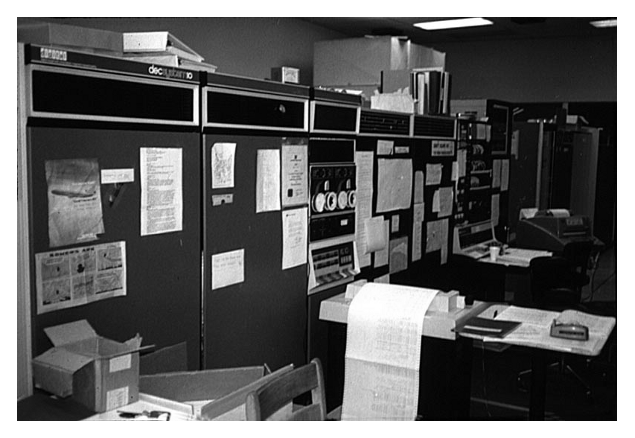
\includegraphics{KL10_1979}
  \caption{PDP-10 processor with KL-10 (a PDP-10 similar to that of the AI Lab), Stanford Artificial Intelligence Laboratory, 1979.}
\end{figure}

``Without hackers to maintain the system, [faculty members] said, `We're going to have a disaster; we must have commercial software,'\hspace{0.01in}'' Stallman would recall a few years later. ``They said, `We can expect the company to maintain it.' It proved that they were utterly wrong, but that's what they did.''\endnote{\textit{Ibid.}}

At first, hackers viewed the Twenex system as yet another authoritarian symbol begging to be subverted. The system's name itself was a protest. Officially dubbed TOPS-20 by DEC, it was named as a successor to TOPS-10, a proprietary operating system DEC distributed for the PDP-10. But TOPS-20 was not based on TOPS-10.  It was derived from the Tenex system which Bolt Beranek Newman had developed for the PDP-10.\endnote{Multiple sources: see Richard Stallman interview, Gerald Sussman email, and \textit{Jargon File 3.0.0} at \url{http://catb.org/jargon/html/T/TWENEX.html}.} Stallman, the hacker who coined the Twenex term, says he came up with the name as a way to avoid using the TOPS-20 name. ``The system was far from tops, so there was no way I was going to call it that,'' Stallman recalls. ``So I decided to insert a `w' in the Tenex name and call it Twenex.''

The machine that ran the Twenex/TOPS-20 system had its own derisive nickname: Oz. According to one hacker legend, the machine got its nickname because it required a smaller PDP-11 machine to power its terminal. One hacker, upon viewing the KL-10-PDP-11 setup for the first time, likened it to the wizard's bombastic onscreen introduction in the Wizard of Oz. ``I am the great and powerful Oz,'' the hacker intoned. ``Pay no attention to the PDP-11 behind that console.''\endnote{See \url{http://www.as.cmu.edu/~geek/humor/See_Figure_1.txt}.}

If hackers laughed when they first encountered the KL-10, their laughter quickly died when they encountered Twenex. Not only did Twenex boast built-in security, but the system's software engineers had designed the tools and applications with the security system in mind. What once had been a cat-and-mouse game over passwords in the case of the Laboratory for Computer Science's security system, now became an out-and-out battle over system management. System administrators argued that without security, the Oz system was more prone to accidental crashes. Hackers argued that crashes could be better prevented by overhauling the source code. Unfortunately, the number of hackers with the time and inclination to perform this sort of overhaul had dwindled to the point that the system-administrator argument prevailed.

The initial policy was that any lab member could have the ``wheel privilege'' to bypass security restrictions.  But anyone who had the ``wheel privilege'' could take it away from anyone else, who would then be powerless to restore it.  This state of affairs tempted a small group of hackers to try to seize total control by canceling the ``wheel privilege'' for all but themselves.

Cadging passwords, and applying the debugger during startup, Stallman successfully foiled these attempts. After the second foiled ``\textit{coup d'état},'' Stallman issued an alert to all the AI Lab personnel.\endnote{See Richard Stallman (1986).}

``There has been another attempt to seize power,'' Stallman wrote. ``So far, the aristocratic forces have been defeated.'' To protect his identity, Stallman signed the message ``Radio Free OZ.''

The disguise was a thin one at best. By 1982, Stallman's aversion to passwords and secrecy had become so well known that users outside the AI Laboratory were using his account from around the ARPAnet -- the research-funded computer network that would serve as a foundation for today's Internet. One such ``tourist'' during the early 1980s was Don Hopkins, a California programmer who learned through the hacking grapevine that all an outsider needed to do to gain access to MIT's vaunted ITS system was to log in under the initials RMS and enter the same three-letter monogram when the system requested a password.

``I'm eternally grateful that MIT let me and many other people use their computers for free,'' says Hopkins. ``It meant a lot to many people.''

This so-called ``tourist'' policy, which had been openly tolerated by MIT management during the ITS years,\endnote{See ``MIT AI Lab Tourist Policy,'' \url{http://www.art.net/~hopkins/Don/text/tourist-policy.html}.} fell by the wayside when Oz became the lab's primary link to the ARPAnet. At first, Stallman continued his policy of repeating his login ID as a password so outside users could have access through his account. Over time, however, Oz's fragility prompted administrators to bar outsiders who, through sheer accident or malicious intent, might bring down the system. When those same administrators eventually demanded that Stallman stop publishing his password, Stallman, citing personal ethics, instead ceased using the Oz system altogether.\endnote{See Richard Stallman (1986).}

``[When] passwords first appeared at the MIT AI Lab I [decided] to follow my belief that there should be no passwords,'' Stallman would later say. ``Because I don't believe that it's really desirable to have security on a computer, I shouldn't be willing to help uphold the security regime.''\endnote{\textit{Ibid.}}

Stallman's refusal to bow before the great and powerful Oz symbolized the growing tension between hackers and AI Lab management during the early 1980s. This tension paled in comparison to the conflict that raged within the hacker community itself. By the time the Decsystem 20 arrived, the hacker community was divided into two camps, LMI and Symbolics.

Symbolics, with its outside investment, recruited various AI Lab hackers and set some of them working on improving parts of the Lisp Machine operating system outside the auspices of the AI Lab. By the end of 1980, the company had hired 14 AI Lab staffers as part-time consultants to develop its version of the Lisp Machine. The remaining few, apart from Stallman, worked for LMI.\endnote{See Steve Levy, \textit{Hackers}, page 423.}  Stallman, preferring the unpressured life at the AI Lab and not wishing to take a side, chose to join neither company.

At first, the other hackers continued spending some of their time at MIT, and contributed to MIT's Lisp Machine operating system. Both LMI and Symbolics had licensed this code from MIT. The license required them to return their changes to MIT, but did not require them to let MIT redistribute these changes.  However, through 1981 they adhered to a gentleman's agreement to permit that, so all their system improvements were included in the MIT version and thus shared with all Lisp Machine users. This situation allowed those still at MIT to remain neutral.

On March 16, 1982, a date Stallman remembers well because it was his birthday, Symbolics executives ended the gentleman's agreement. The motive was to attack LMI. LMI had fewer hackers, and fewer staff in general, so the Symbolics executives thought that LMI was getting the main benefit of sharing the system improvements.  By ending the sharing of system code, they hoped to wipe out LMI.  So they decided to enforce the letter of the license.  Instead of contributing their improvements to the MIT version of the system, which LMI could use, they provided MIT with a copy of the Symbolics version of the system for users at MIT to run.  Anyone using it would provide the service of testing only to Symbolics, and if he made improvements, most likely they too would only be useful for Symbolics.

As the person responsible (with help from Greenblatt for the first couple of months) for keeping up the lab's Lisp Machine system, Stallman was incensed. The Symbolics hackers had left the system code with hundreds of half-made changes that caused errors. Viewing this announcement as an ``ultimatum,'' he retaliated by disconnecting Symbolics' microwave communications link to the laboratory. He then vowed never to work on a Symbolics machine, and pledged to continue the development of MIT's system so as to defend LMI from Symbolics. ``The way I saw it, the AI Lab was a neutral country, like Belgium in World War II,'' Stallman says. ``If Germany invades Belgium, Belgium declares war on Germany and sides with Britain and France.''

When Symbolics executives noticed that their latest features were still appearing in the MIT Lisp Machine system and, by extension, the LMI Lisp machine, they were not pleased. Stallman knew what copyright law required, and was rewriting the features from scratch.  He took advantage of the opportunity to read the source code Symbolics supplied to MIT, so as to understand the problems and fixes, and then made sure to write his changes in a totally different way.  But the Symbolics executives didn't believe this.  They installed a ``spy'' program on Stallman's computer terminal looking for evidence against him.  However, when they took their case to MIT administration, around the start of 1983, they had little evidence to present: a dozen places in the sources where both versions had been changed and appeared similar.

When the AI Lab administrators showed Stallman Symbolics' supposed evidence, he refuted it, showing that the similarities were actually held over from before the fork.  Then he turned the logic around: if, after the thousands of lines he had written, Symbolics could produce no better evidence than this, it demonstrated that Stallman's diligent efforts to avoid copying were effective.  The AI Lab approved Stallman's work, which he continued till the end of 1983.\endnote{\textit{The Brain Makers} by H. P. Newquist says inaccurately that the AI Lab told Stallman to stay away from the Lisp Machine project.}

Stallman did make a change in his practices, though.  ``Just to be ultra safe, I no longer read their source code [for new features and major changes]. I used only the documentation and wrote the code from that.''  For the biggest new features, rather than wait for Symbolics to release documentation, he designed them on his own; later, when the Symbolics documentation appeared, he added compatibility with Symbolics' interface for the feature.  Then he read Symbolics' source code changes to find minor bugs they had fixed, and fixed each of them differently.

The experience solidified Stallman's resolve. As Stallman designed replacements for Symbolics' new features, he also enlisted members of the AI Lab to keep using the MIT system, so as to provide a continuous stream of bug reports. MIT continued giving LMI direct access to the changes. ``I was going to punish Symbolics if it was the last thing I did,'' Stallman says.  Such statements are revealing. Not only do they shed light on Stallman's nonpacifist nature, they also reflect the intense level of emotion triggered by the conflict.

The level of despair owed much to what Stallman viewed as the ``destruction'' of his ``home'' -- i.e., the demise of the AI Lab's close-knit hacker subculture. In a later email interview with Levy, Stallman would liken himself to the historical figure Ishi, the last surviving member of the Yahi, a Pacific Northwest tribe wiped out during the Indian wars of the 1860s and 1870s. The analogy casts Stallman's survival in epic, almost mythical, terms.\endnote{Steven Levy in \textit{Hackers} had this period in mind when he described Stallman as the ``last of the true hackers,'' but his intended meaning was not what you might think.  Levy used the term ``true hackers'' to distinguish the MIT hacker community from two other hacker communities described later in the book, to which he gave other names. When this community had dissolved, leaving only Stallman, he therefore became the last of the ``true hackers.''   Levy did not mean that nobody else was truly a hacker, but people tend to interpret his words that way, especially those who see them without reading the explanations in Levy's book.  Stallman has never described himself using those words of Levy's.} The hackers
who worked for Symbolics saw it differently. Instead of seeing Symbolics as an exterminating force, many of Stallman's colleagues saw it as a belated bid for relevance. In commercializing the Lisp Machine, the company pushed hacker principles of engineer-driven software design out of the ivory-tower confines of the AI Lab and into the corporate marketplace where manager-driven design principles held sway. Rather than viewing Stallman as a holdout, many hackers saw him as the representative of an obsolete practice.

Personal hostilities also affected the situation.   Even before Symbolics hired away most of the AI Lab's hacker staff, Stallman says many of the hackers who later joined Symbolics were shunning him. ``I was no longer getting invited to go to Chinatown,'' Stallman recalls. ``The custom started by Greenblatt was that if you went out to dinner, you went around or sent a message asking anybody at the lab if they also wanted to go. Sometime around 1980-1981, I stopped getting asked. They were not only not inviting me, but one person later confessed that he had been pressured to lie to me to keep their going away to dinner without me a secret.''

Although Stallman felt hurt by this petty form of ostracism, there was nothing to be done about it.  The Symbolics ultimatum changed the matter from a personal rejection to a broader injustice. When Symbolics excluded its source changes from redistribution, as a means to defeat its rival, Stallman determined to thwart Symbolics' goal. By holing up in his MIT offices and writing equivalents for each new software feature and fix, he gave users of the MIT system, including LMI customers, access to the same features as Symbolics users.

It also guaranteed Stallman's legendary status within the hacker community. Already renowned for his work with Emacs, Stallman's ability to match the output of an entire team of Symbolics programmers -- a team that included more than a few legendary hackers itself -- still stands as one of the major human accomplishments of the Information Age, or of any age for that matter. Dubbing it a ``master hack'' and Stallman himself a ``virtual John Henry of computer code,'' author Steven Levy notes that many of his Symbolics-employed rivals had no choice but to pay their idealistic former comrade grudging respect. Levy quotes Bill Gosper, a hacker who eventually went to work for Symbolics in the company's Palo Alto office, expressing amazement over Stallman's output during this period:

\begin{quote}
I can see something Stallman wrote, and I might decide it was bad (probably not, but somebody could convince me it was bad), and I would still say, ``But wait a minute -- Stallman doesn't have anybody to argue with all night over there. He's working alone! It's incredible anyone could do this alone!''\endnote{See Steven Levy, \textit{Hackers} (Penguin USA [paperback], 1984): 426}
\end{quote}

For Stallman, the months spent playing catch up with Symbolics evoke a mixture of pride and profound sadness. As a dyed-in-the-wool liberal whose father had served in World War II, Stallman is no pacifist. In many ways, the Symbolics war offered the rite of passage toward which Stallman had been careening ever since joining the AI Lab staff a decade before. At the same time, however, it coincided with the traumatic destruction of the AI Lab hacker culture that had nurtured Stallman since his teenage years. One day, while taking a break from writing code, Stallman experienced a traumatic moment passing through the lab's equipment room. There, Stallman encountered the hulking, unused frame of the PDP-10 machine. Startled by the dormant lights, lights that once actively blinked out a silent code indicating the status of the internal program, Stallman says the emotional impact was not unlike coming across a beloved family member's well-preserved corpse.

``I started crying right there in the machine room,'' he says. ``Seeing the machine there, dead, with nobody left to fix it, it all drove home how completely my community had been destroyed.''

Stallman would have little opportunity to mourn. The Lisp Machine, despite all the furor it invoked and all the labor that had gone into making it, was merely a sideshow to the large battles in the technology marketplace. The relentless pace of computer miniaturization was bringing in newer, more powerful microprocessors that would soon incorporate the machine's hardware and software capabilities like a modern metropolis swallowing up an ancient desert village.

Riding atop this microprocessor wave were hundreds -- thousands -- of proprietary software programs, each protected by a patchwork of user licenses and nondisclosure agreements that made it impossible for hackers to review or share source code. The licenses were crude and ill-fitting, but by 1983 they had become strong enough to satisfy the courts and scare away would-be interlopers. Software, once a form of garnish most hardware companies gave away to make their expensive computer systems more flavorful, was quickly becoming the main dish. In their increasing hunger for new games and features, users were putting aside the traditional demand to review the recipe after every meal.

Nowhere was this state of affairs more evident than in the realm of personal computer systems. Companies such as Apple Computer and Commodore were minting fresh millionaires selling machines with built-in operating systems. Unaware of the hacker culture and its distaste for binary-only software, many of these users saw little need to protest when these companies failed to attach the accompanying source-code files. A few anarchic adherents of the hacker ethic helped propel that ethic into this new marketplace, but for the most part, the marketplace rewarded the programmers speedy enough to write new programs and savvy enough to write End User License Agreements to lock them up tight.

One of the most notorious of these programmers was Bill Gates, a Harvard dropout two years Stallman's junior. Although Stallman didn't know it at the time, seven years before sending out his message to thenet.unix-wizards newsgroup, Gates, a budding entrepreneur and general partner with the Albuquerque-based software firm Micro-Soft, later spelled as Microsoft, had sent out his own open letter to the software-developer community. Written in response to the PC users copying Micro-Soft's software programs, Gates' ``Open Letter to Hobbyists'' had excoriated the notion of communal software development.

``Who can afford to do professional work for nothing?'' asked Gates. ``What hobbyist can put three man-years into programming, finding all bugs, documenting his product, and distributing it for free?''\endnote{See Bill Gates, ``An Open Letter to Hobbyists'' (February 3, 1976). To view an online copy of this letter, go to \url{http://en.wikipedia.org/wiki/Open_Letter_to_Hobbyists}.}

Although few hackers at the AI Lab saw the missive, Gates' 1976 letter nevertheless represented the changing attitude toward software both among commercial software companies and commercial software developers. Why treat software as a zero-cost commodity when the market said otherwise? As the 1970s gave way to the 1980s, selling software became more than a way to recoup costs; it became a political statement. At a time when the Reagan Administration was rushing to dismantle many of the federal regulations and spending programs that had been built up during the half century following the Great Depression, more than a few software programmers saw the hacker ethic as anticompetitive and, by extension, un-American. At best, it was a throwback to the anticorporate attitudes of the late 1960s and early 1970s. Like a Wall Street banker discovering an old tie-dyed shirt hiding between French-cuffed shirts and double-breasted suits, many computer programmers treated the hacker ethic as an embarrassing reminder of an idealistic age.

For a man who had spent the entire 1960s as a throwback to the 1950s, Stallman didn't mind living out of step with his peers. As a programmer used to working with the best machines and the best software, however, Stallman faced what he could only describe as a ``stark moral choice'': either swallow his ethical objection for ``proprietary'' software -- the term Stallman and his fellow hackers used to describe any program that carried copyright terms or an end-user license that restricted copying and modification -- or dedicate his life to building an alternate, nonproprietary system of software programs. After his two-year battle with Symbolics, Stallman felt confident enough to undertake the latter option. ``I suppose I could have stopped working on computers altogether,'' Stallman says. ``I had no special skills, but I'm sure I could have become a waiter. Not at a fancy restaurant, probably, but I could've been a waiter somewhere.''

Being a waiter -- i.e., dropping out of programming altogether -- would have meant completely giving up an activity, computer programming, that had given him so much pleasure. Looking back on his life since moving to Cambridge, Stallman finds it easy to identify lengthy periods when software programming provided the only pleasure. Rather than drop out, Stallman decided to stick it out.

An Atheist, Stallman rejects notions such as fate, karma, or a divine calling in life. Nevertheless, he does feel that the decision to shun proprietary software and build an operating system to help others do the same was a natural one. After all, it was Stallman's own personal combination of stubbornness, foresight, and coding virtuosity that led him to consider a fork in the road most others didn't know existed. In his article, ``The GNU Project,'' Stallman affirms agreement with the ideals encapsulated in the words of the Jewish sage Hillel:

\begin{quote}
If I am not for myself, who will be for me? If I am only for myself, what am I? If not now, when?\endnote{See \url{http://www.gnu.org/gnu/the-gnu-project.html}. Stallman adds his own footnote to this statement, writing, ``As an Atheist, I don't follow any religious leaders, but I sometimes find I admire something one of them has said.''}
\end{quote}

Speaking to audiences, Stallman avoids the religious route and expresses the decision in pragmatic terms. ``I asked myself: what could I, an operating-system developer, do to improve the situation? It wasn't until I examined the question for a while that I realized an operating-system developer was exactly what was needed to solve the problem.''

Once he recognized that, Stallman says, everything else ``fell into place.'' In 1983, MIT was acquiring second-generation Lisp Machines from Symbolics, on which the MIT Lisp Machine system could not possibly run.  Once most of the MIT machines were replaced, he would be unable to continue maintaining that system effectively for lack of users' bug reports.  He would have to stop.  But he also wanted to stop.  The MIT Lisp Machine system was not free software: even though users could get the source code, they could not redistribute it freely.  Meanwhile, the goal of continuing the MIT system had already been achieved: LMI had survived and was developing software on its own.

Stallman didn't want to spend his whole life punishing those who had destroyed his old community.  He wanted to build a new one. He decided to denounce software that would require him to compromise his ethical beliefs, and devote his life to the creation of programs that would make it easier for him and others to escape from it. Pledging to build a free software operating system ``or die trying -- of old age, of course,'' Stallman quips, he resigned from the MIT staff in January, 1984, to build GNU.

The resignation distanced Stallman's work from the legal auspices of MIT. Still, Stallman had enough friends and allies within the AI Lab to continue using the facilities, and later his own office. He also had the ability to secure outside consulting gigs to underwrite the early stages of the GNU Project. In resigning from MIT, however, Stallman negated any debate about conflict of interest or Institute ownership of the software. The man whose early adulthood fear of social isolation had driven him deeper and deeper into the AI Lab's embrace was now building a legal firewall between himself and that environment.

For the first few months, Stallman operated in isolation from the Unix community as well. Although his announcement to the net.unix-wizards group had attracted sympathetic responses, few volunteers signed on to join the crusade in its early stages.

``The community reaction was pretty much uniform,'' recalls Rich Morin, leader of a Unix user group at the time. ``People said, `Oh, that's a great idea. Show us your code. Show us it can be done.'\hspace{0.01in}''

Aware that the job was enormous, Stallman decided to try to reuse existing free software wherever possible.  So he began looking for existing free programs and tools that could be converted into GNU programs and tools. One of the first candidates was a compiler named VUCK, which converted programs written in the popular C programming language into machine-runnable code. Translated from the Dutch, the program's acronym stood for the Free University Compiler Kit. Optimistic, Stallman asked the program's author if the program was free. When the author informed him that the words ``Free University'' were a reference to the Vrije Universiteit in Amsterdam, and that the program was not free, Stallman was chagrined.

``He responded derisively, stating that the university was free but the compiler was not,'' recalls Stallman. He had not only refused to help -- he suggested Stallman drop his plan to develop GNU, and instead write some add-ons to boost sales of VUCK, in return for a share of the profits. ``I therefore decided that my first program for the GNU Project would be a multi-language, multi-platform compiler.''\endnote{See Richard Stallman, ``The GNU Operating System and the Free Software Movement,'' \textit{Open Sources} (O'Reilly \& Associates, Inc., 1999): 65.}

Instead of VUCK, Stallman found the Pastel compiler (``off-color Pascal''), written by programmers at Lawrence Livermore National Lab. According to what they said when they gave him a copy, the compiler was free to copy and modify. Unfortunately, the program was unsuitable for the job, because its memory requirements were enormous.  It parsed the entire input file in core memory, then retained all the internal data until it finished compiling the file. On mainframe systems this design had been forgivable. On Unix systems it was a crippling barrier, since even 32-bit machines that ran Unix were often unable to provide so much memory to a program. Stallman made substantial progress at first, building a C-compatible frontend to the compiler and testing it on the larger Vax, whose system could handle large memory spaces. When he tried porting the system to the 68010, and investigated why it crashed,  he discovered the memory size problem, and concluded he would have to build a totally new compiler from scratch.  Stallman eventually did this, producing the GNU C Compiler or GCC.  But it was not clear in 1984 what to do about the compiler, so he decided to let those plans gel while turning his attention to other parts of GNU.

In September of 1984, thus, Stallman began development of a GNU version of Emacs, the replacement for the program he had been supervising for a decade. Within the Unix community, the two native editor programs were vi, written by Sun Microsystems cofounder Bill Joy, and ed, written by Bell Labs scientist (and Unix cocreator) Ken Thompson. Both were useful and popular, but neither offered the endlessly expandable nature of Emacs.

Looking back, Stallman says he didn't view the decision in strategic terms. ``I wanted an Emacs, and I had a good opportunity to develop one.''

Once again, Stallman had found existing code with which he hoped to save time. In writing a Unix version of Emacs, Stallman was soon following the footsteps of Carnegie Mellon graduate student James Gosling, author of a C-based version dubbed Gosling Emacs or Gosmacs. Gosling's version of Emacs included an interpreter for a simplified offshoot of the Lisp language, called Mocklisp. Although Gosling had put Gosmacs under copyright and had sold the rights to UniPress, a privately held software company, Stallman received the assurances of a fellow developer who had participated in early Gosmacs development. According to the developer, Gosling, while a Ph.D. student at Carnegie Mellon, had given him permission by email to distribute his own version of Gosmacs in exchange for his contribution to the code.

At first Stallman thought he would change only the user-level commands, to implement full compatibility with the original PDP-10 Emacs.  However, when he found how weak Mocklisp was in comparison with real Lisp, he felt compelled to replace it with a true Lisp system.  This made it natural to rewrite most of the higher-level code of Gosmacs in a completely different way, taking advantage of the greater power and flexible data structures of Lisp.  By mid-1985, in GNU Emacs as released on the Internet, only a few files still had code remaining from Gosmacs.

Then UniPress caught wind of Stallman's project, and denied that the other developer had received permission to distribute his own version of Gosmacs.  He could not find a copy of the old email to defend his claim.  Stallman eliminated this problem by writing replacements for the few modules that remained from Gosmacs.

Nevertheless, the notion of developers selling off software rights -- indeed, the very notion of developers having such powers to sell in the first place -- rankled Stallman. In a 1986 speech at the Swedish Royal Technical Institute, Stallman cited the UniPress incident as yet another example of the dangers associated with proprietary software.

``Sometimes I think that perhaps one of the best things I could do with my life is find a gigantic pile of proprietary software that was a trade secret, and start handing out copies on a street corner so it wouldn't be a trade secret any more,'' said Stallman. ``Perhaps that would be a much more efficient way for me to give people new free software than actually writing it myself; but everyone is too cowardly to even take it.''\endnote{See Richard Stallman (1986).}

Despite the stress it generated, the dispute over Gosling's code would assist both Stallman and the free software movement in the long term. It would force Stallman to address the weaknesses of the Emacs Commune and the informal trust system that had allowed problematic offshoots to emerge. It would also force Stallman to sharpen the free software movement's political objectives. Following the release of GNU Emacs in 1985, Stallman issued \textit{The GNU Manifesto}, an expansion of the original announcement posted in September, 1983. Stallman included within the document a lengthy section devoted to the many arguments used by commercial and academic programmers to justify the proliferation of proprietary software programs. One argument, ``Don't programmers deserve a reward for their creativity,'' earned a response encapsulating Stallman's anger over the recent Gosling Emacs episode:

``If anything deserves a reward, it is social contribution,'' Stallman wrote. ``Creativity can be a social contribution, but only in so far [\textit{sic}] as society is free to use the results. If programmers deserve to be rewarded for creating innovative programs, by the same token they deserve to be punished if they restrict the use of these programs.''\endnote{See Richard Stallman, \textit{The GNU Manifesto} (1985), \url{http://www.gnu.org/gnu/manifesto.html}.}

With the release of GNU Emacs, the GNU Project finally had code to show. It also had the burdens of any software-based enterprise. As more and more Unix developers began playing with the software, money, gifts, and requests for tapes began to pour in. To address the business side of the GNU Project, Stallman drafted a few of his colleagues and formed the Free Software Foundation (FSF), a nonprofit organization dedicated to speeding the GNU Project towards its goal. With Stallman as president and various friends and hacker allies as board members, the FSF helped provide a corporate face for the GNU Project.

Robert Chassell, a programmer then working at Lisp Machines, Inc., became one of five charter board members at the Free Software Foundation following a dinner conversation with Stallman. Chassell also served as the organization's treasurer, a role that started small but quickly grew.

``I think in '85 our total expenses and revenue were something in the order of \$23,000, give or take,'' Chassell recalls. ``Richard had his office, and we borrowed space. I put all the stuff, especially the tapes, under my desk. It wasn't until sometime later LMI loaned us some space where we could store tapes and things of that sort.''

In addition to providing a face, the Free Software Foundation provided a center of gravity for other disenchanted programmers. The Unix market that had seemed so collegial even at the time of Stallman's initial GNU announcement was becoming increasingly competitive. In an attempt to tighten their hold on customers, companies were starting to deny users access to Unix source code, a trend that only speeded the number of inquiries into ongoing GNU software projects. The Unix wizards who once regarded Stallman as a noisy kook were now beginning to see him as a software prophet or a software Cassandra, according as they felt hope or despair over escaping the problems he identified.

``A lot of people don't realize, until they've had it happen to them, how frustrating it can be to spend a few years working on a software program only to have it taken away,'' says Chassell, summarizing the feelings and opinions of the correspondents writing in to the FSF during the early years. ``After that happens a couple of times, you start to say to yourself, `Hey, wait a minute.'\hspace{0.01in}''

For Chassell, the decision to participate in the Free Software Foundation came down to his own personal feelings of loss. Prior to LMI, Chassell had been working for hire, writing an introductory book on Unix for Cadmus, Inc., a Cambridge-area software company. When Cadmus folded, taking the rights to the book down with it, Chassell says he attempted to buy the rights back with no success.

``As far as I know, that book is still sitting on a shelf somewhere, unusable, uncopyable, just taken out of the system,'' Chassell says. ``It was quite a good introduction if I may say so myself. It would have taken maybe three or four months to convert [the book] into a perfectly usable introduction to GNU/Linux today. The whole experience, aside from what I have in my memory, was lost.''

Forced to watch his work sink into the mire while his erstwhile employer struggled through bankruptcy, Chassell says he felt a hint of the anger that drove Stallman to fits of apoplexy. ``The main clarity, for me, was the sense that if you want to have a decent life, you don't want to have bits of it closed off,'' Chassell says. ``This whole idea of having the freedom to go in and to fix something and modify it, whatever it may be, it really makes a difference. It makes one think happily that after you've lived a few years that what you've done is worthwhile. Because otherwise it just gets taken away and thrown out or abandoned or, at the very least, you no longer have any relation to it. It's like losing a bit of your life.''

\bigskip

\theendnotes
\setcounter{endnote}{0}

%% Copyright (c) 2002, 2010 Sam Williams
%% Copyright (c) 2010 Richard M. Stallman
%% Permission is granted to copy, distribute and/or modify this
%% document under the terms of the GNU Free Documentation License,
%% Version 1.3 or any later version published by the Free Software
%% Foundation; with no Invariant Sections, no Front-Cover Texts, and
%% no Back-Cover Texts. A copy of the license is included in the
%% file called ``gfdl.tex''.

\chapter{St. Ignucius}

The Maui High Performance Computing Center is located in a single-story building in the dusty red hills just above the town of Kihei. Framed by million-dollar views and the multimillion dollar real estate of the Silversword Golf Course, the center seems like the ultimate scientific boondoggle. Far from the boxy, sterile confines of Tech Square or even the sprawling research metropolises of Argonne, Illinois and Los Alamos, New Mexico, the MHPCC seems like the kind of place where scientists spend more time on their tans than their post-doctoral research projects.

The image is only half true. Although researchers at the MHPCC do take advantage of the local recreational opportunities, they also take their work seriously. According to \url{Top500.org}, a web site that tracks the most powerful supercomputers in the world, the IBM SP Power3 supercomputer housed within the MHPCC clocks in at 837 billion floating-point operations per second, making it one of 25 most powerful computers in the world. Co-owned and operated by the University of Hawaii and the U.S. Air Force, the machine divides its computer cycles between the number crunching tasks associated with military logistics and high-temperature physics research.

Simply put, the MHPCC is a unique place, a place where the brainy culture of science and engineering and the laid-back culture of the Hawaiian islands coexist in peaceful equilibrium. A slogan on the lab's 2000 web site sums it up: ``Computing in paradise.''

It's not exactly the kind of place you'd expect to find Richard Stallman, a man who, when taking in the beautiful view of the nearby Maui Channel through the picture windows of a staffer's office, mutters a terse critique: ``Too much sun.'' Still, as an emissary from one computing paradise to another, Stallman has a message to deliver, even if it means subjecting his hacker eyes to painful solar glare.

The conference room is already full by the time I arrive to catch Stallman's speech. The gender breakdown is a little better than at the New York speech, 85\% male, 15\% female, but not by much. About half of the audience members wear khaki pants and logo-encrusted golf shirts. The other half seems to have gone native. Dressed in the gaudy flower-print shirts so popular in this corner of the world, their faces are a deep shade of ochre. The only residual indication of geek status are the gadgets: Nokia cell phones, Palm Pilots, and Sony VAIO laptops.

Needless to say, Stallman, who stands in front of the room dressed in plain blue T-shirt, brown polyester slacks, and white socks, sticks out like a sore thumb. The fluorescent lights of the conference room help bring out the unhealthy color of his sun-starved skin.\endnote{RMS: The idea that skin can be ``sun-starved'' or that paleness is ``unhealthy'' is dangerous misinformation; staying out of the sun can't hurt you as long as you have enough Vitamin D. What damages the skin, and can even kill you, is excessive exposure to sunlight.}  His beard and hair are enough to trigger beads of sweat on even the coolest Hawaiian neck. Short of having the words ``mainlander'' tattooed on his forehead, Stallman couldn't look more alien if he tried. [RMS: Is there something bad about looking different from others?]

As Stallman putters around the front of the room, a few audience members wearing T-shirts with the logo of the Maui FreeBSD Users Group (MFUG) race to set up camera and audio equipment. FreeBSD, a free software offshoot of the Berkeley Software Distribution, the venerable 1970s academic version of Unix, is technically a competitor to the GNU/Linux operating system. Still, in the hacking world, Stallman speeches are documented with a fervor reminiscent of the Grateful Dead and its legendary army of amateur archivists. As the local free software heads, it's up to the MFUG members to make sure fellow programmers in Hamburg, Mumbai, and Novosibirsk don't miss out on the latest pearls of RMS wisdom.

The analogy to the Grateful Dead is apt. Often, when describing the business opportunities inherent within the free software model, Stallman has held up the Grateful Dead as an example. In refusing to restrict fans' ability to record live concerts, the Grateful Dead became more than a rock group. They became the center of a tribal community dedicated to Grateful Dead music. Over time, that tribal community became so large and so devoted that the band shunned record contracts and supported itself solely through musical tours and live appearances. In 1994, the band's last year as a touring act, the Grateful Dead drew \$52 million in gate receipts alone.\endnote{See ``Grateful Dead Time Capsule: 1985-1995 North American Tour Grosses,'' \url{http://www.dead101.com/1197.htm}.}

While few software companies have been able to match that success, the tribal aspect of the free software community is one reason many in the latter half of the 1990s started to accept the notion that publishing software source code might be a good thing. Hoping to build their own loyal followings, companies such as IBM, Sun Microsystems, and Hewlett Packard have come to accept the letter, if not the spirit, of the Stallman free software message. Describing the GPL as the information-technology industry's \textit{Magna Carta}, ZDNet software columnist Evan Leibovitch sees the growing affection for all things GNU as more than just a trend. ``This societal shift is letting users take back control of their futures,'' Leibovitch writes. ``Just as the \textit{Magna Carta} gave rights to British subjects, the GPL enforces consumer rights and freedoms on behalf of the users of computer software.''\endnote{See Evan Leibovitch, ``Who's Afraid of Big Bad Wolves,'' \textit{ZDNet Tech Update} (December 15, 2000), \url{http://www.zdnet.com/news/whos-afraid-of-the-big-bad-wolves/298394}.}

The tribal aspect of the free software community also helps explain why 40-odd programmers, who might otherwise be working on physics projects or surfing the Web for windsurfing buoy reports, have packed into a conference room to hear Stallman speak.

Unlike the New York speech, Stallman gets no introduction. He also offers no self-introduction. When the FreeBSD people finally get their equipment up and running, Stallman simply steps forward, starts speaking, and steamrolls over every other voice in the room.

``Most of the time when people consider the question of what rules society should have for using software, the people considering it are from software companies, and they consider the question from a self-serving perspective,'' says Stallman, opening his speech. ``What rules can we impose on everybody else so they have to pay us lots of money? I had the good fortune in the 1970s to be part of a community of programmers who shared software. And because of this I always like to look at the same issue from a different direction to ask: what kind of rules make possible a good society that is good for the people who are in it? And therefore I reach completely different answers.''

Once again, Stallman quickly segues into the parable of the Xerox laser printer, taking a moment to deliver the same dramatic finger-pointing gestures to the crowd. He also devotes a minute or two to the GNU/Linux name.

``Some people say to me, `Why make such a fuss about getting credit for this system? After all, the important thing is the job is done, not whether you get recognition for it.' Well, this would be wise advice if it were true. But the job wasn't to build an operating system; the job is to spread freedom to the users of computers. And to do that we have to make it possible to do everything with computers in freedom.''\endnote{For narrative purposes, I have hesitated to go in-depth when describing Stallman's full definition of software ``freedom.'' The GNU Project web site lists four fundamental components:

\begin{itemize}
  \item The freedom to run the program as you wish, for any purpose (freedom 0).
  \item The freedom to study the program's source code, and change it so that the program does what you wish (freedom 1).
  \item The freedom to redistribute copies of the program so you can help your neighbor (freedom 2).
  \item The freedom to distribute copies of your modified versions, so that the whole community can benefit from them (freedom 3).
\end{itemize}

For more information, please visit ``The Free Software Definition'' at \url{http://www.gnu.org/philosophy/free-sw.html}.}

Adds Stallman, ``There's a lot more work to do.''

For some in the audience, this is old material. For others, it's a little arcane. When a member of the golf-shirt contingent starts dozing off, Stallman stops the speech and asks somebody to wake the person up.

``Somebody once said my voice was so soothing, he asked if I was some kind of healer,'' says Stallman, drawing a quick laugh from the crowd. ``I guess that probably means I can help you drift gently into a blissful, relaxing sleep. And some of you might need that. I guess I shouldn't object if you do. If you need to sleep, by all means do.''

The speech ends with a brief discussion of software patents, a growing issue of concern both within the software industry and within the free software community. Like Napster, software patents reflect the awkward nature of applying laws and concepts written for the physical world to the frictionless universe of information technology.

Copyright law and patent law work differently, and have totally different effects in the software field.  The copyright on a program controls the copying and adaptation of that program's code, and it belongs to the program's developer.  But copyright does not cover ideas. In other words, a developer is free, under copyright, to implement in his own code features and commands he has seen in existing programs.  Those aspects are ideas, not expression, and thus outside the scope of copyright law.

It is likewise lawful -- though hard work -- to decode how a binary program works, and then implement the same ideas and algorithms in different code.  This practice is known as ``reverse engineering.''

Software patents work differently. According to the U.S. Patent Office, companies and individuals can obtain patents for computing ideas that are innovative (or, at least, unknown to the Patent Office). In theory, this allows the patent-holder to trade off disclosure of the technique for a specific monopoly lasting a minimum of 20 years after the patent filing. In practice, the disclosure is of limited value to the public, since the operation of the program is often self-evident, and could in any case be determined by reverse engineering. Unlike copyright, a patent gives its holder the power to forbid the independent development of software programs which use the patented idea.

In the software industry, where 20 years can cover the entire life cycle of a marketplace, patents take on a strategic weight. Where companies such as Microsoft and Apple once battled over copyright and the ``look and feel'' of various technologies, today's Internet companies use patents as a way to stake out individual applications and business models, the most notorious example being Amazon.com's 2000 attempt to patent the company's ``one-click'' online shopping process. For most companies, however, software patents have become a defensive tool, with cross-licensing deals balancing one set of corporate patents against another in a tense form of corporate detente. Still, in a few notable cases of computer encryption and graphic imaging algorithms, software vendors have successfully stifled rival developments.  For instance, some font-rendering features are missing from free software because of patent threats from Apple.

For Stallman, the software-patent issue dramatizes the need for eternal hacker vigilance. It also underlines the importance of stressing the political benefits of free software programs over the competitive benefits. Stallman says competitive performance and price, two areas where free software operating systems such as GNU/Linux and FreeBSD already hold a distinct advantage over their proprietary counterparts, are side issues compared to the large issues of user and developer freedom.

This position is controversial within the community: open source advocates emphasize the utilitarian advantages of free software over the political advantages. Rather than stress the political significance of free software programs, open source advocates have chosen to stress the engineering integrity of the hacker development model. Citing the power of peer review, the open source argument paints programs such as GNU/Linux or FreeBSD as better built, better inspected and, by extension, more trustworthy to the average user.

That's not to say the term ``open source'' doesn't have its political implications. For open source advocates, the term open source serves two purposes. First, it eliminates the confusion associated with the word ``free,'' a word many businesses interpret as meaning ``zero cost.'' Second, it allows companies to examine the free software phenomenon on a technological, rather than ethical, basis. Eric Raymond, cofounder of the Open Source Initiative and one of the leading hackers to endorse the term, explained his refusal to follow Stallman's political path in a 1999 essay, titled ``Shut Up and Show Them the Code'':

\begin{quote}
RMS's rhetoric is very seductive to the kind of people we are. We hackers are thinkers and idealists who readily resonate with appeals to ``principle'' and ``freedom'' and ``rights.'' Even when we disagree with bits of his program, we want RMS's rhetorical style to work; we think it ought to work; we tend to be puzzled and disbelieving when it fails on the 95\% of people who aren't wired like we are.\endnote{See Eric Raymond, ``Shut Up and Show Them the Code,'' online essay, (June 28, 1999), \url{http://www.catb.org/~esr/writings/shut-up-and-show-them.html}.}
\end{quote}

Included among that 95\%, Raymond writes, are the bulk of business managers, investors, and nonhacker computer users who, through sheer weight of numbers, tend to decide the overall direction of the commercial software marketplace. Without a way to win these people over, Raymond argues, programmers are doomed to pursue their ideology on the periphery of society:

\begin{quote}
When RMS insists that we talk about ``computer users' rights,'' he's issuing a dangerously attractive invitation to us to repeat old failures. It's one we should reject -- not because his principles are wrong, but because that kind of language, applied to software, simply does not persuade anybody but us. In fact, it confuses and repels most people outside our culture.\endnote{\textit{Ibid.}}
\end{quote}

Stallman, however, rejects Raymond's premises:

\begin{quote}
Raymond's attempt to explain our failure is misleading because we have not failed.  Our goal is large, and we have a long way to go, but we have also come a long way.

Raymond's pessimistic assertion about the values of non-hackers is an exaggeration.  Many non-hackers are more concerned with the political issues we focus on than with the technical advantages that open source emphasizes.  This often includes political leaders too, though not in all countries.

It was the ethical ideals of free software, not ``better software,'' which persuaded the presidents of Ecuador and Brazil to move government agencies to free software.  They are not geeks, but they understand freedom.
\end{quote}

But the principal flaw in the open source argument, according to Stallman, is that it leads to weaker conclusions.  It convinces many users to run some programs which are free, but does not offer them any reason to migrate entirely to free software.  This partially gives them freedom, but does not teach them to recognize it and value it as such, so they remain likely to let it drop and lose it.  For instance, what happens when the improvement of free software is blocked by a patent?

Most open source advocates are equally, if not more, vociferous as Stallman when it comes to opposing software patents.  So too are most proprietary software developers, since patents threaten their projects too.  However, pointing to software patents' tendency to put areas of software functionality off limits, Stallman contrasts what the free software idea and the open source idea imply about such cases.

``It's not because we don't have the talent to make better software,'' says Stallman. ``It's because we don't have the right. Somebody has prohibited us from serving the public. So what's going to happen when users encounter these gaps in free software? Well, if they have been persuaded by the open source movement that these freedoms are good because they lead to more-powerful reliable software, they're likely to say, `You didn't deliver what you promised. This software's not more powerful. It's missing this feature. You lied to me.' But if they have come to agree with the free software movement, that the freedom is important in itself, then they will say, `How dare those people stop me from having this feature and my freedom too.' And with that kind of response, we may survive the hits that we're going to take as these patents explode.''

Watching Stallman deliver his political message in person, it is hard to see anything confusing or repellent. Stallman's appearance may seem off-putting, but his message is logical. When an audience member asks if, in shunning proprietary software, free software proponents lose the ability to keep up with the latest technological advancements, Stallman answers the question in terms of his own personal beliefs. ``I think that freedom is more important than mere technical advance,'' he says. ``I would always choose a less advanced free program rather than a more advanced nonfree program, because I won't give up my freedom for something like that [advance]. My rule is, if I can't share it with you, I won't take it.''

In the minds of those who assume ethics means religion, such answers reinforce the quasi-religious nature of the Stallman message. However, unlike a Jew keeping kosher or a Mormon refusing to drink alcohol, Stallman is not obeying a commandment, but simply refusing to cede his freedom.  His speech explains the practical requisites for doing so: a proprietary program takes away your freedom, so if you want freedom, you need to reject the program.

Stallman paints his decision to use free software in place of proprietary in the color of a personal belief he hopes others will come to share. As software evangelists go, Stallman avoids forcing those beliefs down listeners' throats. Then again, a listener rarely leaves a Stallman speech not knowing where the true path to software righteousness lies.

As if to drive home this message, Stallman punctuates his speech with an unusual ritual. Pulling a black robe out of a plastic grocery bag, Stallman puts it on.  Then he pulls out a reflective brown computer disk and places it on his head. The crowd lets out a startled laugh.

``I am St. IGNUcius of the Church of Emacs,'' says Stallman, raising his right hand in mock-blessing. ``I bless your computer, my child.''

\begin{figure}[ht] \centering
  \includegraphics{stignucius}
  \caption{Stallman dressed as St. IGNUcius. The photo was taken by Stian Eikeland in Bergen, Norway on February 19, 2009.}
\end{figure}

The laughter turns into full-blown applause after a few seconds. As audience members clap, the computer disk on Stallman's head catches the glare of an overhead light, eliciting a perfect halo effect. In the blink of an eye, Stallman resembles a Russian religious icon.

``Emacs was initially a text editor,'' says Stallman, explaining the getup. ``Eventually it became a way of life for many and a religion for some. We call this religion the Church of Emacs.''

The skit is a lighthearted moment of self-parody, a humorous return-jab at the many people who might see Stallman's form of software asceticism as religious fanaticism in disguise. It is also the sound of the other shoe dropping -- loudly. It's as if, in donning his robe and halo, Stallman is finally letting listeners off the hook, saying, ``It's OK to laugh. I know I'm weird.''  [RMS: To laugh at someone for being weird is boorish, and it is not my intention to excuse that.  But I hope people will laugh at my St. IGNUcius comedy routine.]

Discussing the St. IGNUcius persona afterward, Stallman says he first came up with it in 1996, long after the creation of Emacs but well before the emergence of the ``open source'' term and the struggle for hacker-community leadership that precipitated it. At the time, Stallman says, he wanted a way to ``poke fun at himself,'' to remind listeners that, though stubborn, Stallman was not the fanatic some made him out to be. It was only later, Stallman adds, that others seized the persona as a convenient way to play up his reputation as software ideologue, as Eric Raymond did in an 1999 interview with the Linux.com web site:

\begin{quote}
When I say RMS calibrates what he does, I'm not belittling or accusing him of insincerity. I'm saying that like all good communicators he's got a theatrical streak. Sometimes it's conscious -- have you ever seen him in his St. IGNUcius drag, blessing software with a disk platter on his head? Mostly it's unconscious; he's just learned the degree of irritating stimulus that works, that holds attention without (usually) freaking people out.\endnote{See ``Guest Interview: Eric S. Raymond,'' \textit{Linux.com} (May 18, 1999), \url{http://www.linux.com/interviews/19990518/8/}.}
\end{quote}

Stallman takes issue with the Raymond analysis. ``It's simply my way of making fun of myself,'' he says. ``The fact that others see it as anything more than that is a reflection of their agenda, not mine.''

That said, Stallman does admit to being a ham. ``Are you kidding?'' he says at one point. ``I love being the center of attention.'' To facilitate that process, Stallman says he once enrolled in Toastmasters, an organization that helps members bolster their public-speaking skills and one Stallman recommends highly to others. He possesses a stage presence that would be the envy of most theatrical performers and feels a link to vaudevillians of years past. A few days after the Maui High Performance Computing Center speech, I allude to the 1999 LinuxWorld performance and ask Stallman if he has a Groucho Marx complex -- i.e., the unwillingness to belong to any club that would have him as a member.\endnote{RMS: Williams misinterprets Groucho's famous remark by treating it as psychological.  It was intended as a jab at the overt antisemitism of many clubs, which was why they would refuse him as a member.  I did not understand this either until my mother explained it to me.  Williams and I grew up when bigotry had gone underground, and there was no need to veil criticism of bigotry in humor as Groucho did.} Stallman's response is immediate: ``No, but I admire Groucho Marx in a lot of ways and certainly have been in some things I say inspired by him. But then I've also been inspired in some ways by Harpo.''

The Groucho Marx influence is certainly evident in Stallman's lifelong fondness for punning. Then again, punning and wordplay are common hacker traits. Perhaps the most Groucho-like aspect of Stallman's personality, however, is the deadpan manner in which the puns are delivered. Most come so stealthily -- without even the hint of a raised eyebrow or upturned smile -- you almost have to wonder if Stallman's laughing at his audience more than the audience is laughing at him.

Watching members of the Maui High Performance Computer Center laugh at the St. IGNUcius parody, such concerns evaporate. While not exactly a standup act, Stallman certainly possesses the chops to keep a roomful of engineers in stitches. ``To be a saint in the Church of Emacs does not require celibacy, but it does require making a commitment to living a life of moral purity,'' he tells the Maui audience. ``You must exorcise the evil proprietary operating systems from all your computers, and then install a wholly [holy] free operating system. And then you must install only free software on top of that. If you make this commitment and live by it, then you too will be a saint in the Church of Emacs, and you too may have a halo.''

The St. IGNUcius skit ends with a brief inside joke. On most Unix systems and Unix-related offshoots, the primary competitor program to Emacs is vi, pronounced vee-eye, a text-editing program developed by former UC Berkeley student and current Sun Microsystems chief scientist, Bill Joy. Before doffing his ``halo,'' Stallman pokes fun at the rival program. ``People sometimes ask me if it is a sin in the Church of Emacs to use vi,'' he says. ``Using a free version of vi is not a sin; it is a penance. So happy hacking.''\endnote{The service of the Church of Emacs has developed further since 2001. Users can now join the Church by reciting the Confession of the Faith: ``There is no system but GNU, and Linux is one of its kernels.'' Stallman sometimes mentions the religious ceremony known as the Foobar Mitzvah, the Great Schism between various rival versions of Emacs, and the cult of the Virgin of Emacs (which refers to any person that has not yet learned to use Emacs).  In addition, ``vi vi vi'' has been identified as the Editor of the Beast.}

After a brief question-and-answer session, audience members gather around Stallman. A few ask for autographs. ``I'll sign this,'' says Stallman, holding up one woman's print out of the GNU General Public License, ``but only if you promise me to use the term GNU/Linux instead of Linux'' (when referring to the system), ``and tell all your friends to do likewise.''

The comment merely confirms a private observation. Unlike other stage performers and political figures, Stallman has no ``off'' mode. Aside from the St. IGNUcius character, the ideologue you see onstage is the ideologue you meet backstage. Later that evening, during a dinner conversation in which a programmer mentions his affinity for ``open source'' programs, Stallman, between bites, upbraids his tablemate: ``You mean free software. That's the proper way to refer to it.''

During the question-and-answer session, Stallman admits to playing the pedagogue at times. ``There are many people who say, `Well, first let's invite people to join the community, and then let's teach them about freedom.' And that could be a reasonable strategy, but what we have is almost everybody's inviting people to join the community, and hardly anybody's teaching them about freedom once they come in.''

The result, Stallman says, is something akin to a third-world city. ``You have millions of people moving in and building shantytowns, but nobody's working on step two: getting them out of those shantytowns. If you think talking about software freedom is a good strategy, please join in doing step two. There are plenty working on step one. We need more people working on step two.''

Working on ``step two'' means driving home the issue that freedom, not acceptance, is the root issue of the free software movement. Those who hope to reform the proprietary software industry from the inside are on a fool's errand. ``Change from the inside is risky,'' Stallman stays. ``Unless you're working at the level of a Gorbachev, you're going to be neutralized.''

Hands pop up. Stallman points to a member of the golf shirt-wearing contingent. ``Without patents, how would you suggest dealing with commercial espionage?''

``Well, those two questions have nothing to do with each other, really,'' says Stallman.

``But I mean if someone wants to steal another company's piece of software.''

Stallman's recoils as if hit by a poisonous spray. ``Wait a second,'' Stallman says. ``Steal? I'm sorry, there's so much prejudice in that statement that the only thing I can say is that I reject that prejudice.'' Then he turns to the substance of the question. ``Companies that develop nonfree software and other things keep lots and lots of trade secrets, and so that's not really likely to change. In the old days -- even in the 1980s -- for the most part programmers were not aware that there were even software patents and were paying no attention to them. What happened was that people published the interesting ideas, and if they were not in the free software movement, they kept secret the little details. And now they patent those broad ideas and keep secret the little details. So as far as what you're describing, patents really make no difference to it one way or another.''

``But if it doesn't affect their publication,'' a new audience member jumps in, his voice trailing off almost as soon as he starts speaking.

``But it does,'' Stallman says. ``Their publication is telling you that this is an idea that's off limits to the rest of the community for 20 years. And what the hell good is that? Besides, they've written it in such a hard way to read, both to obfuscate the idea and to make the patent as broad as possible, that it's basically useless looking at the published information [in the patent] to learn anything anyway. The only reason to look at patents is to see the bad news of what you can't do.''

The audience falls silent. The speech, which began at 3:15, is now nearing the 5:00 whistle, and most listeners are already squirming in their seats, antsy to get a jump start on the weekend. Sensing the fatigue, Stallman glances around the room and hastily shuts things down. ``So it looks like we're done,'' he says, following the observation with an auctioneer's ``going, going, gone'' to flush out any last-minute questioners. When nobody throws their hand up, Stallman signs off with a traditional exit line.

``Happy hacking,'' he says.

\theendnotes
\setcounter{endnote}{0}

%% Copyright (c) 2002, 2010 Sam Williams
%% Copyright (c) 2010 Richard M. Stallman
%% Permission is granted to copy, distribute and/or modify this
%% document under the terms of the GNU Free Documentation License,
%% Version 1.3 or any later version published by the Free Software
%% Foundation; with no Invariant Sections, no Front-Cover Texts, and
%% no Back-Cover Texts. A copy of the license is included in the
%% file called ``gfdl.tex''.


\chapter{The GNU General Public License}

By the spring of 1985, Richard Stallman had produced the GNU Project's first useful result -- a Lisp-based version of Emacs for Unix-like operating systems. To make it available to others as free software, he had to develop the way to release it -- in effect, the follow-on for the Emacs Commune.

The tension between the freedom to modify and authorial privilege had been building before Gosmacs. The Copyright Act of 1976 had overhauled U.S. copyright law, extending the legal coverage of copyright to software programs. According to Section 102(b) of the Act, individuals and companies could copyright the ``expression'' of a software program but not the ``actual processes or methods embodied in the program.''\endnote{See Hal Abelson, Mike Fischer, and Joanne Costello, ``Software and Copyright Law,'' updated version (1997), \url{http://groups.csail.mit.edu/mac/classes/6.805/articles/int-prop/software-copyright.html}.}

Translated, this treated a program much like an algebra textbook: its author can claim copyright on the text but not on the mathematical ideas of algebra or the pedagogical technique employed to explain it.  Thus, regardless of what Stallman said about using the code of the original Emacs, other programmers were legally entitled to write their own implementations of the ideas and commands of Emacs, and they did.  Gosmacs was one of 30-odd imitations of the original Emacs developed for various computer systems.

The Emacs Commune applied only to the code of the original Emacs program written by Stallman himself.  Even if it had been legally enforced, it would not have applied to separately developed imitations such as Gosmacs.  Making Gosmacs nonfree was unethical according to the ethical ideas of the free software movement, because (as proprietary software) it did not respect its users' freedom, but this issue had nothing to do with where the ideas in Gosmacs came from.

Under copyright, programmers who wanted to copy code from an existing program (even with changes) had to obtain permission from the original developer. The new law applied copyright even in the absence of copyright notices -- though hackers generally did not know this -- and the copyright notices too began appearing.

Stallman saw these notices as the flags of an invading, occupying army. Rare was the program that didn't borrow source code from past programs, and yet, with a single stroke of the president's pen, the U.S. government had given programmers and companies the legal power to forbid such reuse.  Copyright also injected a dose of formality into what had otherwise been an informal system. Simply put, disputes that had once been settled hacker-to-hacker were now to be settled lawyer-to-lawyer. In such a system, companies, not hackers, held the automatic advantage.  Some saw placing one's name in a copyright notice as taking responsibility for the quality of the code, but the copyright notice usually has a company's name, and there are other ways for individuals to say what code they wrote.

However, Stallman also noticed, in the years leading up to the GNU Project, that copyright allowed an author to grant permission for certain activities covered by copyright, and place conditions on them too.  ``I had seen email messages with copyright notices plus simple `verbatim copying permitted' licenses,'' he recalls. ``Those definitely were [an] inspiration.''  These licenses carried the condition not to remove the license.  Stallman's idea was to take this a few steps further.  For example, a permission notice could allow users to redistribute even modified versions, with the condition that these versions carry the same permission.

Thus Stallman concluded that use of copyright was not necessarily unethical.  What was bad about software copyright was the way it was typically used, and designed to be used: to deny the user essential freedoms.  Most authors imagined no other way to use it.  But copyright could be used in a different way: to make a program free and assure its continued freedom.

By GNU Emacs 16, in early 1985, Stallman drafted a copyright-based license that gave users the right to make and distribute copies. It also gave users the right to make and distribute modified versions, but only under the same license.  They could not exercise the unlimited power of copyright over those modified versions, so they could not make their versions proprietary as Gosmacs was.  And they had to make the source code available.  Those conditions closed the legal gap that would otherwise allow restricted, nonfree versions of GNU Emacs to emerge.

Although helpful in codifying the social contract of the Emacs Commune, the early GNU Emacs license remained too ``informal'' for its purpose, Stallman says. Soon after forming the Free Software Foundation he began working on a more airtight version, consulting with the other directors and with the attorneys who had helped to set it up.

Mark Fischer, a Boston copyright attorney who initially provided Stallman's legal advice, recalls discussing the license with Stallman during this period. ``Richard had very strong views about how it should work,'' Fischer says, ``He had two principles. The first was to make the software absolutely as open as possible.'' (By the time he said this, Fischer seems to have been influenced by open source supporters; Stallman never sought to make software ``open.'') ``The second was to encourage others to adopt the same licensing practices.''  The requirements in the license were designed for the second goal.

The revolutionary nature of this final condition would take a while to sink in. At the time, Fischer says, he simply viewed the GNU Emacs license as a simple trade. It put a price tag on GNU Emacs' use. Instead of money, Stallman was charging users access to their own later modifications. That said, Fischer does remember the license terms as unique.

``I think asking other people to accept the price was, if not unique, highly unusual at that time,'' he says.

In fashioning the GNU Emacs license, Stallman made one major change to the informal tenets of the old Emacs Commune. Where he had once demanded that Commune members send him all the changes they wrote, Stallman now demanded only that they pass along source code and freedom whenever they chose to redistribute the program. In other words, programmers who simply modified Emacs for private use no longer needed to send the source-code changes back to Stallman. In a rare alteration of free software doctrine, Stallman slashed the ``price tag'' for free software. Users could innovate without Stallman looking over their shoulders, and distribute their versions only when they wished, just so long as all copies came with permission for their possessors to develop and redistribute them further.

Stallman says this change was fueled by his own dissatisfaction with the Big Brother aspect of the original Emacs Commune social contract. As much as he had found it useful for everyone to send him their changes, he came to feel that requiring this was unjust.

``It was wrong to require people to publish all changes,'' says Stallman. ``It was wrong to require them to be sent to one privileged developer. That kind of centralization and privilege for one was not consistent with a society in which all had equal rights.''

The GNU Emacs General Public License made its debut on a version of GNU Emacs in 1985. Following the release, Stallman welcomed input from the general hacker community on how to improve the license's language. One hacker to take up the offer was future software activist John Gilmore, then working as a consultant to Sun Microsystems. As part of his consulting work, Gilmore had ported Emacs over to SunOS, the company's in-house version of Unix. In the process of doing so, Gilmore had published the changed version under the GNU Emacs license. Instead of viewing the license as a liability, Gilmore saw it as clear and concise expression of the hacker ethos. ``Up until then, most licenses were very informal,'' Gilmore recalls.

As an example of this informality, Gilmore cites the mid-1980s copyright license of trn, a news reader program written by Larry Wall, a hacker who could go onto later fame as the creator of both the Unix ``patch'' utility and the Perl scripting language. In the hope of striking a balance between common hacker courtesy and an author's right to dictate the means of commercial publication, Wall used the program's accompanying copyright notice as an editorial sounding board.

\begin{quote}
Copyright (c) 1985, Larry Wall\\
You may copy the trn kit in whole or in part as long as you don't try to make money off it, or pretend that you wrote it.\endnote{See Trn Kit README, \url{http://stuff.mit.edu/afs/sipb/project/trn/src/trn-3.6/README}.}
\end{quote}

Such statements, while reflective of the hacker ethic, also reflected the difficulty of translating the loose, informal nature of that ethic into the rigid, legal language of copyright. In writing the GNU Emacs license, Stallman had done more than close up the escape hatch that permitted proprietary offshoots. He had expressed the hacker ethic in a manner understandable to both lawyer and hacker alike.

It wasn't long, Gilmore says, before other hackers began discussing ways to ``port'' the GNU Emacs license over to their own programs. Prompted by a conversation on Usenet, Gilmore sent an email to Stallman in November, 1986, suggesting modification:

\begin{quote}
You should probably remove ``EMACS'' from the license and replace it with ``SOFTWARE'' or something. Soon, we hope, Emacs will not be the biggest part of the GNU system, and the license applies to all of it.\endnote{See John Gilmore, quoted from email to author.}
\end{quote}

Gilmore wasn't the only person suggesting a more general approach. By the end of 1986, Stallman himself was at work with GNU Project's next major milestone, the source-code debugger GDB.  To release this, he had to modify the GNU Emacs license so it applied to GDB instead of GNU Emacs.  It was not a big job, but it was an opening for possible errors.  In 1989, Stallman figured out how to remove the specific references to Emacs, and express the connection between the program code and the license solely in the program's source files.  This way, any developer could apply the license to his program without changing the license. The GNU General Public License, GNU GPL for short, was born.  The GNU Project soon made it the official license of all existing GNU programs.

In publishing the GPL, Stallman followed the software convention of using decimal numbers to indicate versions with minor changes and whole numbers to indicate versions with major changes. The first version, in 1989, was labeled Version 1.0. The license contained a preamble spelling out its political intentions:

\begin{quote}
The General Public License is designed to make sure that you have the freedom to give away or sell copies of free software, that you receive source code or can get it if you want it, that you can change the software or use pieces of it in new free programs; and that you know you can do these things.

To protect your rights, we need to make restrictions that forbid anyone to deny you these rights or to ask you to surrender the rights. These restrictions translate to certain responsibilities for you if you distribute copies of the software, or if you modify it.\endnote{See Richard Stallman, et al., ``GNU General Public License: Version 1,'' (February, 1989), \url{http://www.gnu.org/licenses/old-licenses/gpl-1.0.html}.}
\end{quote}

As hacks go, the GPL stands as one of Stallman's best. It created a system of communal ownership within the normally proprietary confines of copyright law. More importantly, it demonstrated the intellectual similarity between legal code and software code. Implicit within the GPL's preamble was a profound message: instead of viewing copyright law with suspicion, hackers should view it as a dangerous system that could be hacked.

``The GPL developed much like any piece of free software with a large community discussing its structure, its respect or the opposite in their observation, needs for tweaking and even to compromise it mildly for greater acceptance,'' says Jerry Cohen, another attorney who advised Stallman after Fischer departed. ``The process worked very well and GPL in its several versions has gone from widespread skeptical and at times hostile response to widespread acceptance.''

In a 1986 interview with \textit{BYTE} magazine, Stallman summed up the GPL in colorful terms. In addition to proclaiming hacker values, Stallman said, readers should also ``see it as a form of intellectual jujitsu, using the legal system that software hoarders have set up against them.''\endnote{See David Betz and Jon Edwards, ``Richard Stallman discusses his public-domain [\textit{sic}] Unix-compatible software system with \textit{BYTE} editors,'' \textit{BYTE} (July, 1986). (Reprinted on the GNU Project web site: \url{http://www.gnu.org/gnu/byte-interview.html}.)

This interview offers an interesting, not to mention candid, glimpse at Stallman's political attitudes during the earliest days of the GNU Project. It is also helpful in tracing the evolution of Stallman's rhetoric.

Describing the purpose of the GPL, Stallman says, ``I'm trying to change the way people approach knowledge and information in general. I think that to try to own knowledge, to try to control whether people are allowed to use it, or to try to stop other people from sharing it, is sabotage.''

Contrast this with a statement to the author in August 2000: ``I urge you not to use the term `intellectual property' in your thinking. It will lead you to misunderstand things, because that term generalizes about copyrights, patents, and trademarks. And those things are so different in their effects that it is entirely foolish to try to talk about them at once. If you hear somebody saying something 'about intellectual property,' without [putting it in] quotes, then he's not thinking very clearly and you shouldn't join.''

[RMS: The contrast it shows is that I've learned to be more cautious in generalizing.  I probably wouldn't talk about ``owning knowledge'' today, since it's a very broad concept.  But ``owning knowledge'' is not the same generalization as ``intellectual property,'' and the difference between those three laws is crucial to understanding any legal issue about owning knowledge.  Patents are direct monopolies over using specific knowledge; that really is one form of ``owning knowledge.'' Copyrights are one of the methods used to stop the sharing of works that embody or explain knowledge, which is a very different thing. Meanwhile, trademarks have very little to do with the subject of knowledge.]} Years later, Stallman would describe the GPL's creation in less hostile terms. ``I was thinking about issues that were in a sense ethical and in a sense political and in a sense legal,'' he says. ``I had to try to do what could be sustained by the legal system that we're in. In spirit the job was that of legislating the basis for a new society, but since I wasn't a government, I couldn't actually change any laws. I had to try to do this by building on top of the existing legal system, which had not been designed for anything like this.''

About the time Stallman was pondering the ethical, political, and legal issues associated with free software, a California hacker named Don Hopkins mailed him a manual for the 68000 microprocessor. Hopkins, a Unix hacker and fellow science-fiction buff, had borrowed the manual from Stallman a while earlier. As a display of gratitude, Hopkins decorated the return envelope with a number of stickers obtained at a local science-fiction convention. One sticker in particular caught Stallman's eye. It read, ``Copyleft (L), All Rights Reversed.''  Stallman, inspired by the sticker, nicknamed the legal technique employed in the GNU Emacs license (and later in the GNU GPL) ``Copyleft,'' jocularly symbolized by a backwards ``C'' in a circle. Over time, the nickname would become general Free Software Foundation terminology for any copyright license ``making a program free software and requiring all modified and extended versions of the program to be free software as well.''

The German sociologist Max Weber once proposed that all great religions are built upon the ``routinization'' or ``institutionalization'' of charisma. Every successful religion, Weber argued, converts the charisma or message of the original religious leader into a social, political, and ethical apparatus more easily translatable across cultures and time.

While not religious per se, the GNU GPL certainly qualifies as an interesting example of this ``routinization'' process at work in the modern, decentralized world of software development. Since its unveiling, programmers and companies who have otherwise expressed little loyalty or allegiance to Stallman have willingly accepted the GPL bargain at face value. Thousands have also accepted the GPL as a preemptive protective mechanism for their own software programs. Even those who reject the GPL conditions as too limiting still credit it as influential.

One hacker falling into this latter group was Keith Bostic, a University of California employee at the time of the GPL 1.0 release. Bostic's department, the Computer Systems Research Group (SRG), had been involved in Unix development since the late 1970s and was responsible for many key parts of Unix, including the TCP/IP networking protocol, the cornerstone of modern Internet communications. By the late 1980s, AT\&T, the original owner of the Unix software, began to focus on commercializing Unix and began looking to the Berkeley Software Distribution, or BSD, the academic version of Unix developed by Bostic and his Berkeley peers, as a key source of commercial technology.

The code written by Bostic and friends was off limits to nearly everyone, because it was intermixed with proprietary AT\&T code. Berkeley distributions were therefore available only to institutions that already had a Unix source license from AT\&T. As AT\&T raised its license fees, this arrangement, which had at first seemed innocuous (to those who thought only of academia) became increasingly burdensome even there.  To use Berkeley's code in GNU, Stallman would have to convince Berkeley to separate it from AT\&T's code and release it as free software.  In 1984 or 1985 he met with the leaders of the BSD effort, pointing out that AT\&T was not a charity and that for a university to donate its work (in effect) to AT\&T was not proper.  He asked them to separate out their code and release it as free software.

Hired in 1986, Bostic had taken on the personal project of porting the latest version of BSD to the PDP-11 computer. It was during this period, Bostic says, that he came into close interaction with Stallman during Stallman's occasional forays out to the west coast. ``I remember vividly arguing copyright with Stallman while he sat at borrowed workstations at CSRG,'' says Bostic. ``We'd go to dinner afterward and continue arguing about copyright over dinner.''

The arguments eventually took hold, although not in the way Stallman would have preferred. In June, 1989, Berkeley had separated its networking code from the rest of the AT\&T-owned operating system and began distributing it under a copyright-based free license. The license terms were liberal. All a licensee had to do was give credit to the university in advertisements touting derivative programs.\endnote{The University of California's ``obnoxious advertising clause'' would later prove to be a problem. Looking for a permissive alternative to the GPL, some hackers used the original BSD license, replacing ``University of California'' with their own names or the names of their institutions. The result: free software systems using many of these programs would have to cite dozens of names in advertisements. In 1999, after a few years of lobbying on Stallman's part, the University of California agreed to drop this clause. See ``The BSD License Problem'' at \url{http://www.gnu.org/philosophy/bsd.html}.} In contrast to the GPL, this license permitted proprietary offshoots.  One problem limited the use of the BSD Networking release: it wasn't a complete operating system, just the network-related parts of one.  While the code would be a major contribution to any free operating system, it could only be run at that time in conjunction with other, proprietary-licensed code.

Over the next few years, Bostic and other University of California employees worked to replace the missing components and turn BSD into a complete, freely redistributable operating system. Although delayed by a legal challenge from Unix Systems Laboratories -- the AT\&T spin-off that retained ownership of the Unix code -- the effort would finally bear fruit in the early 1990s. Even before then, however, many of the Berkeley network utilities would make their way into Stallman's GNU system.

``I think it's highly unlikely that we ever would have gone as strongly as we did without the GNU influence,'' says Bostic, looking back. ``It was clearly something where they were pushing hard and we liked the idea.''

By the end of the 1980s, the GPL was beginning to exert a gravitational effect on the free software community. A program didn't have to carry the GPL to qualify as free software -- witness the case of the BSD network utilities -- but putting a program under the GPL sent a definite message. ``I think the very existence of the GPL inspired people to think through whether they were making free software, and how they would license it,'' says Bruce Perens, creator of Electric Fence, a popular Unix utility, and future leader of the Debian GNU/Linux development team. A few years after the release of the GPL, Perens says he decided to discard Electric Fence's homegrown license in favor of Stallman's lawyer-vetted copyright. ``It was actually pretty easy to do,'' Perens recalls.

Rich Morin, the programmer who had viewed Stallman's initial GNU announcement with a degree of skepticism, recalls being impressed by the software that began to gather under the GPL umbrella. As the leader of a SunOS user group, one of Morin's primary duties during the 1980s had been to send out distribution tapes containing the best freeware or free software utilities. The job often mandated calling up original program authors to verify whether their programs were copyrighted or whether they had been consigned to the public domain. Around 1989, Morin says, he began to notice that the best software programs typically fell under the GPL license. ``As a software distributor, as soon as I saw the word GPL, I knew I was home free,'' recalls Morin.

To compensate for the prior hassles that went into compiling distribution tapes to the Sun User Group, Morin had charged recipients a convenience fee. Now, with programs moving over to the GPL, Morin was suddenly getting his tapes put together in half the time, turning a tidy profit in the process. Sensing a commercial opportunity, Morin rechristened his hobby as a business: Prime Time Freeware.

Such commercial exploitation was completely consistent with the free software agenda. ``When we speak of free software, we are referring to freedom, not price,'' advised Stallman in the GPL's preamble. By the late 1980s, Stallman had refined it to a more simple mnemonic: ``Don't think free as in free beer; think free as in free speech.''

For the most part, businesses ignored Stallman's entreaties. Still, for a few entrepreneurs, the freedom associated with free software was the same freedom associated with free markets. Take software ownership out of the commercial equation, and you had a situation where even the smallest software company was free to compete against the IBMs and DECs of the world.

One of the first entrepreneurs to grasp this concept was Michael Tiemann, a software programmer and graduate student at Stanford University. During the 1980s, Tiemann had followed the GNU Project like an aspiring jazz musician following a favorite artist. It wasn't until the release of the GNU C Compiler, or GCC, in 1987, however, that he began to grasp the full potential of free software. Dubbing GCC a ``bombshell,'' Tiemann says the program's own existence underlined Stallman's determination as a programmer.

``Just as every writer dreams of writing the great American novel, every programmer back in the 1980s talked about writing the great American compiler,'' Tiemman recalls. ``Suddenly Stallman had done it. It was very humbling.''

``You talk about single points of failure, GCC was it,'' echoes Bostic. ``Nobody had a compiler back then, until GCC came along.''

Rather than compete with Stallman, Tiemann decided to build on top of his work. The original version of GCC weighed in at 110,000 lines of code, but Tiemann recalls the program as surprisingly easy to understand. So easy in fact that Tiemann says it took less than five days to master and another week to port the software to a new hardware platform, National Semiconductor's 32032 microchip. Over the next year, Tiemann began playing around with the source code, creating the first ``native'' or direct compiler for the C++ programming language, by extending GCC to handle C++ as well as C. (The existing, proprietary implementation of the C++ language worked by converting the code to the C language, then feeding the result to a C compiler.) One day, while delivering a lecture on the program at Bell Labs, Tiemann ran into some AT\&T developers struggling to pull off the same thing.

``There were about 40 or 50 people in the room, and I asked how many people were working on the native code compiler,'' Tiemann recalls. ``My host said the information was confidential but added that if I took a look around the room I might get a good general idea.''

It wasn't long after, Tiemann says, that the light bulb went off in his head. ``I had been working on that project for six months,'' Tiemann says. I just thought to myself, whether it's me or the code, this is a level of efficiency that the free market should be ready to reward.''

Tiemann found added inspiration in the \textit{GNU Manifesto}: while excoriating the greed of proprietary software vendors, it also encourages companies, as long as they respect users freedom, to use and redistribute free software in their commercial activities. By removing the power of monopoly from the commercial software question, the GPL makes it possible for even small companies to compete on the basis of service, which extends from simple tech support to training to extending free programs for specific clients' needs.

In a 1999 essay, Tiemann recalls the impact of Stallman's \textit{Manifesto}. ``It read like a socialist polemic, but I saw something different. I saw a business plan in disguise.''\endnote{See Michael Tiemann, ``Future of Cygnus Solutions: An Entrepreneur's Account,'' \textit{Open Sources} (O'Reilly \& Associates, Inc., 1999): 139, \url{http://www.oreilly.com/catalog/opensources/book/tiemans.html}.}

This business plan was not new; Stallman supported himself in the late 80s by doing this on a small scale.  But Tiemann intended to take it to a new level.
Teaming up with John Gilmore and David Vinayak Wallace, Tiemann launched a software consulting service dedicated to customizing GNU programs. Dubbed Cygnus Support (informally, ``Cygnus'' was a recursive acronym for ``Cygnus, Your GNU Support''), the company signed its first development contract in February, 1990. By the end of the year, the company had \$725,000 worth of support and development contracts.

The complete GNU operating system Stallman envisioned required more than software development tools.  In the 1990s, GNU also developed a command line interpreter or ``shell,'' which was an extended replacement for the Bourne Shell (written by FSF employee Brian Fox, and christened by Stallman the Bourne Again Shell, or BASH), as well as the PostScript interpreter Ghostscript, the documentation browser platform Texinfo, the C Library which C programs need in order to run and talk to the system's kernel, the spreadsheet Oleo (``better for you than the more expensive spreadsheet''), and even a fairly good chess game.  However, programmers were typically most interested in the GNU programming tools.

GNU Emacs, GDB, and GCC were the ``big three'' of developer-oriented tools, but they weren't the only ones developed by the GNU Project in the 80s. By 1990, GNU had also generated GNU versions of the build-controller Make, the parser-generator YACC (rechristened Bison), and awk (rechristened gawk); as well as dozens more. Like GCC, GNU programs were usually designed to run on multiple systems, not just a single vendor's platform. In the process of making programs more flexible, Stallman and his collaborators often made them more useful as well.

Recalling the GNU universalist approach, Prime Time Freeware's Morin points to a useless but vitally important software package called GNU Hello, which serves as an example to show programmers how to properly package a program for GNU. ``It's the hello world program which is five lines of C, packaged up as if it were a GNU distribution,'' Morin says. ``And so it's got the Texinfo stuff and the configure stuff. It's got all the other software engineering goo that the GNU Project has come up with to allow packages to port to all these different environments smoothly. That's tremendously important work, and it affects not only all of [Stallman's] software, but also all of the other GNU Project software.''

According to Stallman, improving technically on the components of Unix was secondary to replacing them with free software. ``With each piece I may or may not find a way to improve it,'' said Stallman to \textit{BYTE}. ``To some extent I am getting the benefit of reimplementation, which makes many systems much better. To some extent it's because I have been in the field a long time and worked on many other systems. I therefore have many ideas [which I learned from them] to bring to bear.''\endnote{See Richard Stallman, \textit{BYTE} (1986).}

Nevertheless, as GNU tools made their mark in the late 1980s, Stallman's AI Lab-honed reputation for design fastidiousness soon became legendary throughout the entire software-development community.

Jeremy Allison, a Sun user during the late 1980s and programmer destined to run his own free software project, Samba, in the 1990s, recalls that reputation with a laugh. During the late 1980s, Allison began using Emacs. Inspired by the program's community-development model, Allison says he sent in a snippet of source code only to have it rejected by Stallman.

``It was like the \textit{Onion} headline,'' Allison says. ``\hspace{0.01in}`Child's prayers to God answered: No.'\hspace{0.01in}''

As the GNU Project moved from success to success in creation of user-level programs and libraries, it postponed development of the kernel, the central ``traffic cop'' program that controls other programs' access to the processor and all machine resources.

As with several other major system components, Stallman sought a head-start on kernel development by looking for an existing program to adapt. A review of GNU Project ``GNUsletters'' of the late 1980s reveals that this approach, like the initial attempt to build GCC out of Pastel, had its problems. A January, 1987 GNUsletter reported the GNU Project's intention to overhaul TRIX, a kernel developed at MIT. However, Stallman never actually tried to do this, since he was working on GCC at the time; later he concluded that TRIX would require too much change to be a good starting point. By February of 1988, according to a newsletter published that month, the GNU Project had shifted its kernel plans to Mach, a lightweight ``micro-kernel'' developed at Carnegie Mellon. Mach was not then free software, but its developers privately said they would liberate it; when this occurred, in 1990, GNU Project kernel development could really commence.\endnote{See ``Hurd History,'' \url{http://www.gnu.org/software/hurd/history.html}.}

The delays in kernel development were just one of many concerns weighing on Stallman during this period. In 1989, Lotus Development Corporation filed suit against rival software companies, Paperback Software International and Borland, for copying menu commands from Lotus' popular 1-2-3 Spreadsheet program. Lotus' suit, coupled with the Apple-Microsoft ``look and feel'' battle, endangered the future of the GNU system. Although neither suit directly attacked the GNU Project, both threatened the right to develop software compatible with existing programs, as many GNU programs were.  These lawsuits could impose a chilling effect on the entire culture of software development. Determined to do something, Stallman and a few professors put an ad in \textit{The Tech} (the MIT student newspaper) blasting the lawsuits and calling for a boycott of both Lotus and Apple. He then followed up the ad by helping to organize a group to protest the corporations filing the suit. Calling itself the League for Programming Freedom, the group held protests outside the offices of Lotus, Inc.

The protests were notable.\endnote{According to a League for Programming Freedom press release at \url{http://progfree.org/Links/prep.ai.mit.edu/demo.final.release}, the protests were notable for featuring the first hexadecimal protest chant:

\begin{verse}
1-2-3-4, toss the lawyers out the door\\
5-6-7-8, innovate don't litigate\\
9-A-B-C, 1-2-3 is not for me\\
D-E-F-O, look and feel have got to go\\
\end{verse}}

They document the evolving nature of the software industry. Applications had quietly replaced operating systems as the primary corporate battleground. In its unfinished quest to build a free software operating system, the GNU Project seemed hopelessly behind the times to those whose primary values were fashion and success. Indeed, the very fact that Stallman had felt it necessary to put together an entirely new group dedicated to battling the ``look and feel'' lawsuits led some observers to think that the FSF was obsolete.

However, Stallman had a strategic reason to start a separate organization to fight the imposition of new monopolies on software development: so that proprietary software developers would join it too.  Extending copyright to cover interfaces would threaten many proprietary software developers as well as many free software developers.  These proprietary developers were unlikely to endorse the Free Software Foundation, but there was, intentionally, nothing in the League for Programming Freedom to drive them away.  For the same reason, Stallman handed over leadership of LPF to others as soon as it was feasible.

In 1990, the John D. and Catherine T. MacArthur Foundation certified Stallman's genius status when it granted Stallman a MacArthur fellowship, the so-called ``genius grant,'' amounting in this case to \$240,000 over 5 years. Although the Foundation does not state a reason for its grants, this one was seen as an award for launching the GNU Project and giving voice to the free software philosophy.  The grant relieved a number of short-term concerns for Stallman.  For instance, it enabled him to cease the consulting work through which he had obtained his income in the 80s and devote more time to the free software cause.

The award also made it possible for Stallman to register normally to vote. In 1985 a fire in the house where Stallman lived left him without an official domicile.  It also covered most of his books with ash, and cleaning these ``dirty books'' did not yield satisfying results. From that time he lived as a ``squatter'' at 545 Technology Square, and had to vote as a ``homeless person.''\endnote{See Reuven Lerner, ``Stallman wins \$240,000 MacArthur award,'' MIT, \textit{The Tech} (July 18, 1990), \url{http://the-tech.mit.edu/V110/N30/rms.30n.html}.} ``[The Cambridge Election Commission] didn't want to accept that as my address,'' Stallman would later recall. ``A newspaper article about the MacArthur grant said that, and then they let me register.''\endnote{See Michael Gross, ``Richard Stallman: High School Misfit, Symbol of Free Software, MacArthur-certified Genius'' (1999).}

Most importantly, the MacArthur fellowship gave Stallman press attention and speaking invitations, which he used to spread the word about GNU, free software, and dangers such as ``look and feel'' lawsuits and software patents.

Interestingly, the GNU system's completion would stem from one of these trips. In April 1991, Stallman paid a visit to the Polytechnic University in Helsinki, Finland. Among the audience members was 21-year-old Linus Torvalds, who was just beginning to develop the Linux kernel -- the free software kernel destined to fill the GNU system's main remaining gap.

A student at the nearby University of Helsinki at the time, Torvalds regarded Stallman with bemusement. ``I saw, for the first time in my life, the stereotypical long-haired, bearded hacker type,'' recalls Torvalds in his 2001 autobiography \textit{Just for Fun}. ``We don't have much of them in Helsinki.''\endnote{See Linus Torvalds and David Diamond, \textit{Just For Fun: The Story of an Accidentaly Revolutionary} (HarperCollins Publishers, Inc., 2001): 58-59. Although presumably accurate in regard to Torvalds' life, what the book says about Stallman is sometimes wrong.  For instance, it says that Stallman ``wants to make everything open source,'' and that he ``complains about other people not using the GPL.''  In fact, Stallman advocates free software, not open source.  He urges authors to choose the GNU GPL, in most circumstances, but says that all free software licenses are ethical.}

While not exactly attuned to the ``sociopolitical'' side of the Stallman agenda, Torvalds nevertheless appreciated one aspect of the agenda's underlying logic: no programmer writes error-free code. Even when users have no wish to adapt a program to their specific preferences, any program can use improvement. By sharing software, hackers put a program's improvement ahead of individual motivations such as greed or ego protection.

Like many programmers of his generation, Torvalds had cut his teeth not on mainframe computers like the IBM 7094, but on a motley assortment of home-built computer systems. As a university student, Torvalds had made the step up from PC programming to Unix, using the university's MicroVAX. This ladder-like progression had given Torvalds a different perspective on the barriers to machine access. For Stallman, the chief barriers were bureaucracy and privilege. For Torvalds, the chief barriers were geography and the harsh Helsinki winter. Forced to trek across the University of Helsinki just to log in to his Unix account, Torvalds quickly began looking for a way to log in from the warm confines of his off-campus apartment.

Torvalds was using Minix, a lightweight nonfree system developed as an instructional example by Dutch university professor Andrew Tanenbaum.\endnote{It was non-free in 1991.  Minix is free software now.} It included the non-free Free University Compiler Kit, plus utilities of the sort that Tanenbaum had contemptuously invited Stallman in 1983 to write.\endnote{Tanenbaum describes Minix as an ``operating system'' in his book, \textit{Operating System Design and Implementation}, but what the book discusses is only the part of the system that corresponds to the kernel of Unix.  There are two customary usages of the term ``operating system,'' and one of them is what is called the ``kernel'' in Unix terminology.  But that's not the only terminological complication in the subject.  That part of Minix consists of a microkernel plus servers that run on it, a design of the same kind as the GNU Hurd plus Mach.  The microkernel plus servers are comparable to the kernel of Unix. but when that book says ``the kernel,'' it refers to the microkernel only.  See Andrew Tanenbaum, \textit{Operating System Design and Implementation}, 1987.}

Minix fit within the memory confines of Torvalds' 386 PC, but it was intended more to be studied than used.  The Minix system also lacked the facility of terminal emulation, which would mimic a typical display terminal and thus enable Torvalds to log in to the MicroVAX from home.

Early in 1991, Torvalds began writing a terminal emulation program.  He used Minix to develop his emulator, but the emulator didn't run on Minix; it was a stand-alone program.  Then he gave it features to access disk files in Minix's file system.  Around then, Torvalds referred to his evolving work as the ``GNU/Emacs of terminal emulation programs.''\endnote{See Linus Torvalds and David Diamond, \textit{Just For Fun: The Story of an Accidentaly Revolutionary} (HarperCollins Publishers, Inc., 2001): 78.}

Since Minix lacked many important features. Torvalds began extending his terminal emulator into a kernel comparable to that of Minix, except that it was monolithic.  Feeling ambitious, he solicited a Minix newsgroup for copies of the POSIX standards, the specifications for a Unix-compatible kernel.\endnote{POSIX was subsequently extended to include specifications for many command line features, but that did not exist in 1991.} A few weeks later, having put his kernel together with some GNU programs and adapted them to work with it, Torvalds was posting a message reminiscent of Stallman's original 1983 GNU posting:

\begin{quote}
Hello everybody out there using minix-

I'm doing a (free) operating system (just a hobby, won't be big and professional like gnu) for 386 (486) AT clones. This has been brewing since April, and is starting to get ready. I'd like any feedback on things people like/dislike in minix, as my OS resembles it somewhat (same physical layout of the file-system (due to practical reasons) among other things).  I've currently ported bash (1.08) and gcc (1.40)\ldots\endnote{\textit{Ibid, p. 85.}}
\end{quote}

The posting drew a smattering of responses and within a month, Torvalds had posted a 0.01 version of his kernel -- i.e., the earliest possible version fit for outside review -- on an Internet FTP site. In the course of doing so, Torvalds had to come up with a name for the new kernel. On his own PC hard drive, Torvalds had saved the program as Linux, a name that paid its respects to the software convention of giving each Unix variant a name that ended with the letter X. Deeming the name too ``egotistical,'' Torvalds changed it to Freax, only to have the FTP site manager change it back.

Torvalds said he was writing a free operating system, and his comparing it with GNU shows he meant a complete system.  However, what he actually wrote was a kernel, pure and simple. Torvalds had no need to write more than the kernel because, as he knew, the other needed components were already available, thanks to the developers of GNU and other free software projects.  Since the GNU Project wanted to use them all in the GNU system, it had perforce made them work together.  While Torvalds continued developing the kernel, he (and later his collaborators) made those programs work with it too.

Initially, Linux was not free software: the license it carried did not qualify as free, because it did not allow commercial distribution. Torvalds was worried that some company would swoop in and take Linux away from him.  However, as the growing GNU/Linux combination gained popularity, Torvalds saw that sale of copies would be useful for the community, and began to feel less worried about a possible takeover.\endnote{\textit{Ibid, p. 94-95.}} This led him to reconsider the licensing of Linux.

Neither compiling Linux with GCC nor running GCC with Linux required him legally to release Linux under the GNU GPL, but Torvalds' use of GCC implied for him a certain obligation to let other users borrow back. As Torvalds would later put it: ``I had hoisted myself up on the shoulders of giants.''\endnote{\textit{Ibid, p. 95-97.}} Not surprisingly, he began to think about what would happen when other people looked to him for similar support. A decade after the decision, Torvalds echoes the Free Software Foundation's Robert Chassell when he sums up his thoughts at the time:

\begin{quote}
You put six months of your life into this thing and you want to make it available and you want to get something out of it, but you don't want people to take advantage of it. I wanted people to be able to see [Linux], and to make changes and improvements to their hearts' content. But I also wanted to make sure that what I got out of it was to see what they were doing. I wanted to always have access to the sources so that if they made improvements, I could make those improvements myself.\endnote{See Linus Torvalds and David Diamond, \textit{Just For Fun: The Story of an Accidentaly Revolutionary} (HarperCollins Publishers, Inc., 2001): 94-95.}
\end{quote}

When it was time to release the 0.12 version of Linux, the first to operate fully with GCC, Torvalds decided to throw his lot in with the free software movement. He discarded the old license of Linux and replaced it with the GPL. Within three years, Linux developers were offering release 1.0 of Linux, the kernel; it worked smoothly with the almost complete GNU system, composed of programs from the GNU Project and elsewhere.  In effect, they had completed the GNU operating system by adding Linux to it.  The resulting system was basically GNU plus Linux.  Torvalds and friends, however, referred to it confusingly as ``Linux.''

By 1994, the amalgamated system had earned enough respect in the hacker world to make some observers from the business world wonder if Torvalds hadn't given away the farm by switching to the GPL in the project's initial months. In the first issue of \textit{Linux Journal}, publisher Robert Young sat down with Torvalds for an interview. When Young asked the Finnish programmer if he felt regret at giving up private ownership of the Linux source code, Torvalds said no. ``Even with 20/20 hindsight,'' Torvalds said, he considered the GPL ``one of the very best design decisions'' made during the early stages of the Linux project.\endnote{See Robert Young, ``Interview with Linus, the Author of Linux,'' \textit{Linux Journal} (March 1, 1994), \url{http://www.linuxjournal.com/article/2736}.}

That the decision had been made with zero appeal or deference to Stallman and the Free Software Foundation speaks to the GPL's growing portability. Although it would take a couple of years to be recognized by Stallman, the explosiveness of Linux development conjured flashbacks of Emacs. This time around, however, the innovation triggering the explosion wasn't a software hack like Control-R but the novelty of running a Unix-like system on the PC architecture. The motives may have been different, but the end result certainly fit the ethical specifications: a fully functional operating system composed entirely of free software.

As his initial email message to the comp.os.minix newsgroup indicates, it would take a few months before Torvalds saw Linux as anything more than a holdover until the GNU developers delivered on the Hurd kernel. As far as Torvalds was concerned, he was simply the latest in a long line of kids taking apart and reassembling things just for fun. Nevertheless, when summing up the runaway success of a project that could have just as easily spent the rest of its days on an abandoned computer hard drive, Torvalds credits his younger self for having the wisdom to give up control and accept the GPL bargain.

``I may not have seen the light,'' writes Torvalds, reflecting on Stallman's 1991 Polytechnic University speech and his subsequent decision to switch to the GPL. ``But I guess something from his speech sunk in.''\endnote{See Linus Torvalds and David Diamond, \textit{Just For Fun: The Story of an Accidentaly Revolutionary} (HarperCollins Publishers, Inc., 2001): 59.}

\theendnotes
\setcounter{endnote}{0}

%% Copyright (c) 2002, 2010 Sam Williams
%% Copyright (c) 2010 Richard M. Stallman
%% Permission is granted to copy, distribute and/or modify this
%% document under the terms of the GNU Free Documentation License,
%% Version 1.3 or any later version published by the Free Software
%% Foundation; with no Invariant Sections, no Front-Cover Texts, and
%% no Back-Cover Texts. A copy of the license is included in the
%% file called ``gfdl.tex''.


\chapter{GNU/Linux}

К 1993 году движение за свободное ПО оказалось на перепутье. Оптимисты упиваются успехом -- хакерская культура заняла место под солнцем, популярность её растёт. Свежие выпуски журнала \textit{Wired} с отвязными статьями про шифрование, Usenet и свободу софта расхватывают, как горячие пирожки. Термин \enquote{интернет} из жаргона хакеров, инженеров и учёных бесповоротно переехал в повседневную лексику. Даже президент Клинтон нередко упоминает его в своих речах о насущных задачах страны. Персональный компьютер был когда-то игрушкой хакеров и гиков, но теперь это атрибут солидности и успеха. Созданные хакерами программы служат миллионам пользователей. Да, проект GNU пока не достиг своей конечной цели -- полностью свободной операционной системы GNU. Но у людей есть свободная система GNU/Linux, совмещающая окружение GNU и ядро Linux.

Всё хорошо, как ни крути. После десятилетий борьбы хакеры утвердили свои ценности, и люди приняли их.

Или нет? Есть люди, что находят массу поводов для пессимизма. Ну да, хакеры теперь на гребне волны, но хорошо ли это для других людей? Да, Белый дом в восторге от интернета и даже открыл официальный сайт whitehouse.gov, но в то же время обсуждает с бизнесом, юристами и полицией как бы взять под контроль этот информационный фронтир, новый Дикий Запад -- всемирную сеть. Да, мощности персональных компьютеров сказочно выросли, но из-за Intel на ПК господствуют несвободные программы. На каждого пользователя GNU/Linux приходятся десятки, а то и сотни пользователей несвободной Windows. Что неудивительно, если взглянуть на графические интерфейсы GNU/Linux -- неудобные и куцые. Работать в них может только очень искушённый человек, как минимум специалист. В создании графического интерфейса проект GNU терпит неудачу.

Над свободным ПО висит грозовая туча авторского права. Продолжаются судебные тяжбы из-за интерфейсов, а число патентов растёт изо дня в день. И похоже что законы, которые создали такую ситуацию, вот-вот введут во многих других странах мира.

Наконец, не всё ладно и в GNU/Linux. Есть юридические проблемы (с ними уже столкнулась BSD), да и сами разработчики ядра Linux не представляют себе, что делать и куда идти. GNU/Linux растёт очень бурно и завоёвывает популярность, но всё ещё больше похож на сборник хитов программирования вроде GCC, Glibc и GDB, чем на цельную операционную систему. Линус Торвальдс и его сподвижники не думают о каком-то плане развития ядра. Торвальдс теперь больше управляет, чем пишет код. Как он сам говорит о своём успехе: \enquote{Я вообще очень ленивый и люблю поручать свою работу другим людям}.\endnote{Такие слова можно найти во многих интервью Торвальдса. Ярчайший пример -- в статье Эрика Реймонда \enquote{Собор и базар} (март 1997 года), \url{http://www.catb.org/~esr/writings/cathedral-bazaar/}.}

Такая лень удивительна с точки зрения продуктивности Линуса, но с политической точки зрения она удручает. Она показывает, что Торвальдсу нет дела до свободы ПО. Он создал и развивает ядро просто ради удовольствия, чего даже не скрывает. Так что же такое GNU/Linux, чем он должен стать? Воплощением философии свободного софта, что выражена в \textit{Манифесте GNU}? Или техничным сочетанием мощных программ, конструктором инструментов для опытных пользователей?

На исходе 1993 года стало понятно, что чаша весов клонится ко второму варианту. Пользователи вовсю создают свои варианты системы -- \enquote{дистрибутивы} GNU/Linux самых разных типов, раздают их бесплатно или продают. Результаты противоречивы.

\enquote{Тогда ещё не было Red Hat и других коммерческих дистрибутивов, -- вспоминает Ян Мёрдок, студент-информатик университета Пердью, -- на всех ресурсах, посвящённых Unix, висели россыпи объявлений со словом \enquote{Linux}. Многие эти компании были однодневками, и не видели ничего плохого в том, чтобы добавить в систему сколько угодно собственнического кода}.

Мёрдок -- программист Unix. Он впервые установил GNU/Linux на домашний компьютер и в полном восторге от системы. \enquote{Это чистейшее удовольствие. Я захотел поучаствовать в общем веселье}. Мёрдока огорчает засилье криво собранных, нестабильных дистрибутивов. Он решает собрать версию системы без каких-либо сомнительных дополнений, и только из лучших образцов свободных программ. \enquote{Хотелось чего-то, что может гордо называться Линуксом}, -- говорит он.

Что делали великие хакеры, собираясь основать великие проекты? Писали в Usenet, пытаясь заинтересовать людей и привлечь их к работе. То же делает и Мёрдок -- пишет о своих намерениях в группу comp.os.linux. И в числе первых ответов видит письмо с адреса \url{rms@ai.mit.edu}. Каждый хакер знает, чей это адрес, знает это и Мёрдок. Это письмо от Ричарда Столлмана -- \enquote{хакера хакеров} и основателя проекта GNU. Что, интересно, ему понадобилось от Мёрдока? Почему культовый хакер, командующий разработкой собственной операционной системы, отозвался на недовольство Мёрдока дистрибутивами \enquote{Linux}?

\enquote{Он сказал, что фонд свободного ПО начал присматриваться к Linux, чтобы, может быть, создать собственную систему Linux [\textit{sic}]. Столлман посчитал, что мои цели сходятся с их философией}.

Без всякого преувеличения, письмо знаменовало изменение стратегии Столлмана. До 1993 года он почти не обращал внимания на Linux. Когда Ричард услышал о первом выпуске ядра, он спросил знакомого хакера о качествах Линукса. Тот ответил, что Linux скроен по образу и подобию System V -- низкопробной версии Unix, и добавил, что Линукс непереносим на другие платформы.

Знакомый хакер всё правильно сказал. Тогда, в 1991 году, ядро Linux работало только на процессорах семейства Intel 386, и выглядело как копия Unix для бедных. Но теперь многое изменилось. Linux оказался единственным свободным ядром операционной системы, и пока Столлман слушал отчёты о неторопливой работе над Hurd, Торвальдс с сотнями сподвижников захватывали компьютерный рынок с его многообразием платформ.

Наступает 1993 год, проект GNU лихорадит. Разработка ядра Hurd замедляется всё сильнее из-за большого числа проблем. Журнал \textit{Wired} пишет, что проект GNU \enquote{увяз}, хотя многие его продукты очень популярны. \endnote{Simson Garfinkel, \enquote{Is Stallman Stalled?} \textit{Wired} (March, 1993).} Но журнал ещё мягок в формулировках, на самом деле настрой у разработчиков проекта ещё хуже. Успех уже готового свободного ядра Linux подкосил мотивацию хакеров. \enquote{Очевидно, что нами двигало желание заполнить пробел в свободной операционной системе, -- вспоминает Часселл, -- и как только пробел заполнился, нам стало не так интересно работать}. \endnote{Часселл считал, что у проекта GNU есть \enquote{окно} размером в 36 месяцев, чтобы представить свою операционную систему, после чего проект станет бессмысленным. И не он один так думал. Несмотря на то, что многие считали различные варианты BSD вроде FreeBSD или OpenBSD более быстрыми, стабильными и безопасными, чем GNU/Linux, эти системы так и не смогли привлечь заметное число пользователей, навсегда оставшись в тени Линукса. То же произошло и с GNU/Hurd. Сравнительный анализ популярности GNU/Linux и других свободных систем в 90-е годы можно посмотреть в эссе новозеландского хакера Лиама Гринвуда: \enquote{Почему Linux популярен} (1999), \url{http://www.freebsddiary.org/linux.php}.}

Уйма работы участников проекта GNU с 1990 по 1993 год пропадает впустую. Многие возлагают вину на Столлмана, но его старый друг Эрик Реймонд считает, что проблема куда глубже. \enquote{Фонд свободного ПО оторвался от жизни в своих амбициях, -- говорит он, -- вместо создания операционной системы он занялся исследованием операционных систем. И что ещё хуже, они думали, что происходящее за пределами фонда не повлияет на них}.

Мёрдок мягче в оценках: \enquote{По-моему, тут сыграло роль то, что они питали слабость к глобальным решениям, не обращая внимания на их эффективность. Например, микроядра -- на рубеже 80-90-х годов они считались решением всех бед, и проект GNU стал разрабатывать именно микроядро. А теперь, когда проблемы микроядер очевидны, уже слишком много сделано, чтобы выбрасывать всё и начинать с нуля}.

Столлман отвечает на это: \enquote{Мнение Реймонда опирается на воображаемые посылки, но в одном он прав: Hurd действительно пошёл не по тому пути разработки. Вместо того, чтобы как можно быстрее сделать рабочее ядро, разработчики постоянно переписывают его огромными кусками, снова и снова, чтобы довести до идеала. Может быть, это и хорошо с академической точки зрения, но очень плохо с практической}.

Ссылается Столлман и на другие проблемы. Судебные войны, развязанные Apple и Lotus, отняли у него много времени и сил, плюс ещё заболевание рук сильно затруднило набор текста, так что Ричард пишет очень мало кода. Отдельная головная боль -- согласованность разных частей проекта GNU. \enquote{Мы потратили очень много сил на GDB, -- говорит Столлман, -- и люди, что им занимались с самого начала, неохотно берутся за другие задачи}. Они предпочитают дальше разрабатывать GDB и помогать пользователям этой программы, глобальная цель проекта GNU их уже мало интересует.

Но самой жестокой проблемой Столлман называет сложность разработки микроядра, которую хакеры GNU очень сильно недооценили поначалу. \enquote{Отлично, мы наладили взаимодействие микроядра Mach с аппаратными ресурсами, -- вспоминает Ричард, -- и кажется, что теперь-то работа пойдёт быстрее. Но не тут-то было. Оказалось, настоящие сложности -- там, где микроядро асинхронно и многопоточно взаимодействует с программами. Начались сплошные ошибки синхронизации, которые портят файлы, и это ни черта не весело. Мы убили столько времени и сил, чтобы получить очень далёкую от готовности систему}.\endnote{Источник -- речь Столлмана в центре высокопроизводительных вычислений Мауи.

После этой речи я написал Столлману письмо, в котором просил объяснить, что означают эти \enquote{ошибки синхронизации}. Столлман ответил, что это лучший способ выразить суть проблем с их микроядром, и объяснил это так:

\begin{quote}
\enquote{Ошибки синхронизации} возникают в системах, где разные части выполняются параллельно, независимо друг от друга. Они могут выполняться в произвольном порядке, и некоторые порядки приводят к проблемам.

Представьте, что программа А делает X, а программа В делает Y, где X и Y это короткие процедуры, меняющие одну и ту же структуру данных. Когда компьютер делает сначала X, а потом Y, или наоборот -- проблем нет. Но может случиться и так, что планировщик ядра запускает программу А, в середине процедуры X он её останавливает и запускает программу B с её процедурой Y. Получается, что Y выполнен полностью, а X -- только наполовину. Но они работают с одной и той же структурой данных, что приводит к противоречию. Например, X может прочитать эту структуру в свою память и работать с нею, но Y в конце своей работы меняет эту структуру, о чём X и не подозревает, продолжая работать с уже несуществующей структурой данных. Как минимум это гарантирует сбой программы А, причём этот сбой очень трудно воспроизвести, ведь он зависит от массы случайных факторов (например, от того, в каком порядке и на какое время планировщик ядра решит запускать программы).

Такие сбои предотвращают блокировкой, которая исключает запуск процедуры Y, пока не закончила работать процедура X. Но разработчики асинхронных систем часто не реализуют блокировки в конкретных местах по недосмотру или из-за лени. И потому множатся ошибки синхронизации.
\end{quote}}

Стало понятно, что проект GNU должен запрыгнуть в уходящий поезд -- не ждать ядро Hurd, а сконцентрироваться на комбинации программ GNU и ядра Linux. Однако это спорный шаг -- сообщество GNU/Linux довольно проблемно с точки зрения философии свободного ПО. Хотя само ядро лицензировано под GPL, многие представители сообщества не стремятся к полностью свободной операционной системе. На конец 1993 года численность пользователей GNU/Linux колеблется от 20 до 100 тысяч человек. \endnote{Это число может быть лишь приблизительным, отсюда такой разброс. Так, о 100 тысячах пользователей сообщал сайт компании Red Hat.} Linux вырос из игрушки в серьёзное ядро, и теперь готов к промышленному использованию, и многие не видят ничего плохого в том, чтобы запускать на нём несвободные программы. Неудивительно, что Столлман смотрит на \enquote{победу} GNU/Linux со смешанными чувствами -- наверное, так же Черчилль смотрел на победу над Гитлером, видя советскую армию в Берлине.\endnote{Позже Столлман прислал мне комментарий насчёт этого сравнения с Черчиллем:

\begin{quote}
Вторая мировая война и связанная с ней воля к победе были очень сильными чувствами, когда я рос. Заявления Черчилля вроде \enquote{мы будем биться с ними на суше, мы будем биться с ними на побережье\ldots и никогда не сдадимся} всегда волновали меня.
\end{quote}}

Столлман опоздал к пирушке победителей, но всё ещё очень влиятелен. Фонд свободного ПО объявляет о финансовой и моральной поддержке проекта Мёрдока, и вслед за этим его окатывает волна поддержки из других источников. Мёрдок называет свой проект Debian -- сокращение от имени его жены Деборы и его собственного имени Ян -- и уже через несколько недель выкатывает первую версию дистрибутива. \enquote{Поддержка Ричарда буквально катапультирует Debian к пику внимания сообщества}, -- говорит Мёрдок.

В январе 1994 года Мёрдок составляет \textit{Манифест Debian}. В духе столлмановского \textit{Манифеста GNU} он объясняет важность тесного сотрудничества с фондом свободного ПО:

\begin{quote}
Фонд свободного программного обеспечения чрезвычайно важен для будущего проекта Debian. Тот простой факт, что этот фонд распространяет дистрибутив, говорит миру, что Linux [\textit{sic}] -- не коммерческий продукт, и не должен быть таковым, но не значит, что Linux не может соперничать с коммерческими продуктами. Если вы не согласны с этим -- объясните рационально успех GNU Emacs и GCC, которые не относятся к коммерческим продуктам, но серьёзно влияют на рынок по факту.

Пришло время позаботиться о будущем Linux [\textit{sic}], а не о деструктивном обогащении за счёт Linux и его сообщества. Может быть, разработка и раздача Debian не решат поднятой в \textit{Манифесте} проблемы, но, надеюсь, хотя бы привлечёт к ней достаточно внимания.\endnote{Ian Murdock, \textit{A Brief History of Debian}, (January 6, 1994): \enquote{The Debian Manifesto,} \url{http://www.debian.org/doc/manuals/project-history/ap-manifesto.en.html}.}
\end{quote}

Вскоре после выхода \textit{Манифеста} фонд свободного ПО делает первый важный запрос. Столлман просит Мёрдока называть систему \enquote{GNU/Linux}. Сначала, впрочем, Ричард предлагает комбинированный вариант -- \enquote{Lignux}, но это название никому не нравится, и Столлман возвращается к более длинному, но не такому критикуемому названию GNU/Linux.

Мёрдок принимает просьбу Столлмана, однако многие продолжают игнорировать приставку \enquote{GNU}, считая её попыткой запоздало приписать себе заслуги. Сам Мёрдок так не считает. По его словам, это попытка примирить разработчиков проекта GNU с теми программистами, что адаптируют программы GNU к ядру Linux. \enquote{Был серьёзный раскол, -- вспоминает он, -- и он беспокоил Ричарда}.

В 1990 году у каждой программы GNU уже был сопровождающий специалист. Многие программы GNU могут работать в разных операционных системах, и пользователи регулярно добавляют в код этих программ возможности для работы на других системах. Но многие пользуются лишь одной операционной системой, и их правки кода часто вызывают проблемы на других платформах. Сопровождающие отклоняют такие правки, прося переделать их. Если пользователь хочет, чтобы его правки попали в общую версию, то ему приходится выполнять требования сопровождающего. После чего сопровождающий принимает правки и далее обслуживает их уже сам. Эта процедура в различных программах GNU повторяется десятки раз для десятков различных систем.

Но программистов, работающих над адаптацией программ GNU к ядру Linux, волнует лишь их собственная система. Когда сопровождающие GNU просят их переделать правки для стабильной работы в других системах, те игнорируют просьбы. Их не заботит правильность кода с точки зрения многоплатформенности и дальнейшей поддержки программ GNU. Они скорее выделят разработку программы в новую ветку, не связанную с проектом GNU, чем будут тратить время на проблемы GNU.

Ветвление разработки программы для хакера -- неоднозначное действие. Конечно, хакерская этика не ограничивает программиста в возможности копировать код и создавать новые версии программ, но хакеры считают более правильным отсылать все правки кода разработчику оригинальной версии. Улучшать сообща основную версию программы удобнее и полезнее для всех. Свободные лицензии не запрещают создавать ответвления, но делать это без явной необходимости считается дурным тоном.

На посту лидера проекта GNU Столлман уже сталкивался с печальными последствиями ветвления кода. В 1991 году компания Lucid нанимает несколько программистом для улучшения GNU Emacs, они пишут ряд новых функций и предлагают их Столлману. Как это обычно бывает, половину этих функций Ричард принимает, а другую половину отклоняет. Программисты настаивают на том, чтобы Столлман принял все функции, но он говорит, что может принять лишь половину, да и то лишь после доработки. Тогда программисты Lucid вообще отказываются помогать ему даже с этой одобренной половиной функций, и ветвят код GNU Emacs, выпуская собственную версию -- Lucid Emacs. Это вызывает бурю эмоций в сообществе.\endnote{Джейми Завински, бывший программист компании Lucid, впоследствии ставший главой разработчиков Mozilla, аргументированно защитил создание Lucid Emacs в статье \enquote{The Lemacs/FSFmacs Schism.}, at \url{http://www.jwz.org/doc/lemacs.html}. Столлман ответил на эти аргументы собственной статьёй здесь \url{http://stallman.org/articles/xemacs.origin}.}

Теперь же программисты делают ответвления сразу нескольких важнейших программ GNU. Поначалу Столлман считает, что так проявляется лихорадочная нетерпеливость, которая характерна для всего динамичного сообщества Linux. В отличие от них, сопровождающие проекта GNU вносят изменения куда медленнее и вдумчивее, анализируя их с точки зрения долгосрочной стабильности. Но со временем, читая электронные письма программистов GNU/Linux, Ричард понимает, что причина в расхождении их целей с целями проекта GNU.

\enquote{Мы видим, что людям, которые называют себя \enquote{пользователями Linux}, неинтересен проект GNU, -- рассказывает Столлман, -- они говорят: \enquote{Почему я должен этим заниматься? Мне плевать на GNU. У меня программа работает, у других пользователей Linux она работает, а остальное нас не волнует}. Удивительно -- люди используют одну из версий системы GNU, и им всё равно на проблемы GNU}. Называя систему \enquote{Линуксом}, они сами себя запутали и забыли, что их система больше GNU, чем Linux.

Ради того, чтобы сохранить единство свободного сообщества, Столлман просит сопровождающих делать то, что должны делать разработчики -- исправлять правки кода в пользу поддержки множества платформ. Как правило, это помогает, но с glibc такой номер не проходит. GNU C Library, glibc -- стандартная библиотека языка С во многих системах. Через неё общаются программы с ядром системы -- так было заведено в Unix, так заведено в Unix-подобных системах. Понятное дело, что в разных системах это общение через glibc проходит по-разному, но во всех системах glibc должна работать одинаково хорошо.

Разработчики Linux адаптируют glibc к своему ядру и предлагают массу изменений в эту библиотеку -- как обычно, очень \enquote{эгоистичных} изменений, учитывающих только их ядро. Сопровождающий glibc говорит, что исправить их все слишком сложно, и тогда фонд свободного ПО нанимает его почти на год, чтобы он с нуля воссоздал функциональность для Линукса. Так появляется 6 версия glibc, для которой GNU/Linux уже \enquote{родная} система.

Именно после этого Столлман настаивает, чтобы в название системы Debian добавили приставку GNU. \enquote{Нам удалось избавиться от другой ветки glibc, но уже понятно, что сообщество Linux может в любой момент пойти своим путём}, -- говорит Мёрдок.

Многие считают, что называть комплект программ GNU и ядра Linux \enquote{вариантом} GNU -- потакать алчной политике, но Мёрдок уже открыто симпатизирует проекту GNU. Он говорит, что просьба Столлмана справедлива. \enquote{Это больше желание сохранить единство, чем отдать почести}.

После этого начался поток просьб технического характера. Мёрдок, полностью соглашаясь с GNU в политике, жёстко возражает Столлману в проектировании и разработке программ. Солидарность тонет в разногласиях.

\enquote{Признаться, мы с ним постоянно спорили, -- смеётся Мёрдок, -- работать с Ричардом бывает трудно}. Так, они принципиально не согласны друг с другом касательно отладки. Столлман хочет включить отладочную информацию во все программы, чтобы пользователям легче было находить ошибки. Мёрдок считает, что это сделает программы большими и медленными. Уступать не хочет никто.

В 1996 году Мёрдок заканчивает университет и передаёт правление растущим проектом Debian в руки Брюса Перенса -- хакера, который создал программу Electric Fence для Unix. Перенс, как и Мёрдок, влюбился в GNU/Linux, как только попробовал его. Как и Мёрдок, он симпатизирует проекту GNU, хотя и не так сильно.

\enquote{После того, как Столлман выпускает \textit{Манифест GNU}, создаёт GNU Emacs и GCC, я вдруг читаю статью, где говорится, что он работает консультантом в Intel, -- вспоминает Перенс первый контакт со Столлманом в конце 80-х годов, -- я пишу ему, мол, как ты можешь бороться за свободу ПО и работать при этом в Intel? Он отвечает мне только: \enquote{Я консультирую их насчёт свободного ПО}. Исчерпывающий и вежливый ответ}.

Перенс -- выдающийся разработчик, и его тревожат баталии Мёрдока и Столлмана о программировании. Став лидером проекта, он решает дистанцировать Debian от фонда свободного ПО. \enquote{Я думаю, нам ни к чему микроменеджмент Ричарда}.

Столлман озадачен и огорчён этим, но теперь он воспринимает это с мудрой сдержанностью. Выждав время, чтобы все остыли, Ричард пишет Перенсу, что не стоит рвать отношения, и что просит лишь называть систему GNU/Linux, больше ничего. \enquote{Я решил, что это хорошо, и согласился, -- говорит Перенс, -- все вздохнули с облегчением}.

Идут годы, и Debian получает репутацию хакерской версии GNU/Linux, подобной Slackware. Но в Slackware есть несвободные программы, и Debian после отхода от GNU тоже включает в коллекции программ собственнический софт. Хотя он явно помечен как nonfree или несвободный, и вынесен в отдельную секцию, предлагать такие программы -- всё равно, что одобрять их. Проект GNU больше не может рекомендовать Debian и Slackware людям.

Но вне хакерских сообществ это всё мало кому интересно. GNU/Linux захватывает рынок, который когда-то занимал Unix. В Северной Каролине появляется компания Red Hat и начинает строить бизнес исключительно на основе GNU/Linux. Исполнительный директор Red Hat -- Роберт Янг, именно он в интервью \textit{Linux Journal} спросил Торвальдса, не жалеет ли тот о переводе ядра под GPL. Уверенный ответ Линуса впечатлил Янга настолько, что он пересмотрел свои представления о Линуксе. Янг задумался, нельзя ли создать компанию на основе того же, что делает Debian -- поставки свободного ПО. Ведь в 1990 году Майкл Тиманн и Джон Гилмор создали компанию Cygnus Solutions, которая зарабатывает на поддержке свободных программ. Может, у Red Hat тоже получится заработать на поддержке GNU/Linux?

\enquote{Западная научная традиция гласит, что мы стоим на плечах гигантов, -- говорит Янг, повторяя слова Торвальдса и Ньютона, -- бизнес тоже говорит, что не нужно изобретать колесо, чтобы двигаться вперёд. Прелесть GPL в том, что вы помещаете код в общественное достояние. \endnote{Здесь Янг слишком вольно притянул \enquote{общественное достояние}, которое вообще означает \enquote{не защищённое авторским правом}. GPL требует, чтобы код был защищён авторским правом, поэтому код под GPL не может быть общественным достоянием.} Допустим, вы независимый производитель софта, и вам для своего приложения нужна программа дозвона. Зачем создавать её заново? Просто используйте программу PPP из Red Hat Linux. Нужна графическая библиотека? Берите GTK. Так вы получаете уже готовые компоненты, причём самые качественные компоненты на рынке. И вы больше не тратите силы и деньги на воссоздание инструментов с нуля. Вы сразу решаете задачи клиентов}. Впрочем, Янг тоже не прочь включить собственнические программы в систему.

Янг -- не единственный, кого волнуют деловой потенциал свободного ПО. Осенью 1996 года компании вовсю принюхиваются к аппетитным запахам с кухни открытого программного кода. Процессор Intel 386, глобальная сеть и веб-сайты накатили на рынок огромными волнами, но всего через год или два накатит настоящее цунами в виде GNU/Linux. Её приближение некоторые чувствуют уже сейчас.

Для Мёрдока это цунами видится и наградой, и наказанием Столлману -- человеку, который столько лет своей жизни вложил в движение за свободное ПО. Как и многие пользователи Linux, Мёрдок помнит, с чего всё начиналось. Как Торвальдс говорил, что изначально Linux был \enquote{просто игрушкой}, и как признавался Таненбауму, что если бы тогда появилось ядро GNU, то он быстро забросил бы Linux. \endnote{Это цитата из знаменитого \enquote{флейма} Торвальдса и Таненбаума, что разгорелся после выхода ядра Linux. Защищая свой выбор монолитного ядра, Торвальдс писал, что делал Linux, чтобы получше изучить свой компьютер. \enquote{Если бы ядро GNU было готово прошлой весной, я бы и не подумал делать своё ядро}. Источник: Chris DiBona, \textit{Open Sources} (O'Reilly \& Associates, Inc., 1999): 224.} Мёрдок видит, как много возможностей упущено. И как ещё больше возможностей находят люди из глубин интернета.

\enquote{Работать над Linux в первые годы было весело, -- вспоминает Мёрдок, -- с другой стороны, с ним работали, чтобы только переждать, пока не появится ядро Hurd -- это видно, если почитать обсуждения в группе comp.os.minix. Если бы Hurd появился быстрее, о Linux бы все забыли}.

Но вот кончился 1996 год, и любые \enquote{если бы} потеряли смысл. Окно размером в 36 месяцев захлопнулось, и теперь даже если появится ядро Hurd, оно останется в тени Linux. Шансы, что его заметит кто-то кроме гиков, очень малы. Linux как будто бы выполнил задачу проекта GNU, заняв последний пробел свободной операционной системы. Только для большинства пользователей вся эта система -- Линукс. На их компьютерах стоят несвободные программы, и они не видят в этом ничего плохого.

И всё-таки мечта хакеров GNU сбылась -- полностью свободная система существует, как бы тернист ни был путь пользователя к ней.

\theendnotes
\setcounter{endnote}{0}

%% Copyright (c) 2002, 2010 Sam Williams
%% Copyright (c) 2010 Richard M. Stallman
%% Permission is granted to copy, distribute and/or modify this
%% document under the terms of the GNU Free Documentation License,
%% Version 1.3 or any later version published by the Free Software
%% Foundation; with no Invariant Sections, no Front-Cover Texts, and
%% no Back-Cover Texts. A copy of the license is included in the
%% file called ``gfdl.tex''.


\chapter{Открытый код} \label{chapter:open source}

[РМС: В этой главе я позволил себе удалить кое-что -- текст, который рассказывал об открытом коде и не имел отношения к моей жизни или работе.]

В ноябре 1995 года Питер Салус, член фонда свободного ПО и автор книги \textit{A Quarter Century of Unix}, обращается к участникам \enquote{системных обсуждений} почтовой рассылки проекта GNU. Он приглашает их в Кембридж, на конференцию по свободно распространяемому программному обеспечению. Конференция эта планируется на февраль 1996 года, спонсируется фондом свободного ПО, и председательствовать на ней будет сам Питер Салус. Она должна стать первой конференцией, полностью посвящённой свободным программам. На конференцию приглашают разработчиков и пользователей всех крупных свободных проектов: GNU, Linux, FreeBSD, NetBSD, 386BSD, Perl, Tcl/Tk -- всех программ, чей код свободно доступен для чтения, редактирования и раздачи. Вот что пишет Салус:

\begin{quote}
За последние 15 лет свободное и бесплатное ПО стало повсеместным. Эта конференция соберёт разработчиков и дистрибьюторов свободных программ. Планируются консультации, учебные лекции, доклады -- в частности, от Линуса Торвальдса и Ричарда Столлмана.\endnote{Peter Salus, \enquote{FYI-Conference on Freely Redistributable Software, 2/2, Cambridge} (1995), \url{http://bat8.inria.fr/~lang/hotlist/free/licence/fsf96/call-for-papers.html}.}
\end{quote}

Один из тех, кто получил письмо Салуса -- Эрик Реймонд. Он не возглавляет какой-либо проект или компанию, как другие адресаты, но у него неплохая репутация среди хакеров. Главным образом, благодаря участию в свободных проектах и составлению \textit{The New Hacker's Dictionary} (\enquote{Нового словаря хакеров})  -- значительно расширенной версии \textit{The Hacker's Dictionary} (\enquote{Словаря хакеров}) за авторством Гая Стила.

Реймонд очень ждёт конференцию, хоть и не полностью согласен с идеями движения за свободное ПО. Ранее он участвовал в разработке некоторых программ GNU, в частности, GNU Emacs. Участие сошло на нет в 1992 году, после того как Реймонд попросил внести его правки кода в официальную версию GNU Emacs, не обсуждая их со Столлманом. Столлман отверг эту просьбу, и Реймонд обвинил Столлмана в \enquote{микроменеджменте}. \enquote{Ричард поднял шум из-за моих несанкционированных чисток Lisp-библиотек Emacs, -- рассказывает Реймонд, -- меня это так расстроило, что я решил никогда больше с ним не работать}.

Несмотря на это, Реймонд активно участвует в жизни сообщества свободного ПО. Настолько активно, что горячо поддерживает идею Салуса провести конференцию, где наравне выступили бы Ричард Столлман и Линус Торвальдс. Столлман представляет старое, умудрённое опытом поколение хакеров, вскормленных ITS и Unix, тогда как Торвальдс -- олицетворение новой волны Линукс-хакеров. Их совместное выступление покажет единство сообщества, что вдохновит многих, особенно из молодёжи -- например, хакеров вроде Реймонда. \enquote{Я как будто синтез обоих поколений}, -- говорит Реймонд.

Необходимость в такой конференции уже давно назрела из-за ощутимого напряжения между двумя поколениями хакеров. Однако обе группы сходятся кое в чём: им всем хочется узреть финского \textit{вундеркинда} во плоти. К их удивлению, Торвальдс окажется приветливым и очаровательным оратором с живым, самокритичным остроумием и лёгким шведским акцентом. \endnote{Торвальдс родился и жил в Финляндии, но его родной язык -- шведский. \enquote{The Rampantly Unofficial Linus FAQ} at \url{http://catb.org/~esr/faqs/linus/} даёт краткие пояснения на этот счёт:

\begin{quote}
В Финляндии живёт немало шведоязычного населения, около 6\% от общей численности. Они называют себя \textit{finlandssvensk} или \textit{finlandssvenskar} и считают себя финнами; многие из таких семей живут в Финляндии веками. Шведский язык -- один из двух официальных языков Финляндии.
\end{quote}}

Ещё большее удивление, по словам Реймонда, вызывает готовность Торвальдса кидать камни в огород именитых хакеров, включая признанного \enquote{хакера хакеров} Ричарда Столлмана. К концу конференции тонкая дерзость Торвальдса одерживает моральную победу над обоими поколениями хакеров.

\enquote{Это был переломный момент, -- вспоминает Реймонд, -- до 1996 года Столлман был единственным заслуживающим доверия кандидатом на роль лидера хакерской культуры. Да, многие не соглашались с ним, но не публично. Торвальдс же отступился от этого правила}.

На исходе конференции Торвальдс окончательно ломает все негласные табу. Идёт обсуждение растущего рыночного господства Microsoft Windows, и Торвальдс заявляет, что одно время был фанатом программы Microsoft PowerPoint. В глазах хакеров старой школы это всё равно, что хвастаться своими рабами на съезде аболиционистов. Но для Торвальдса и молодого поколения хакеров это просто здравый смысл. Зачем ради принципа избегать удобных собственнических программ? Производители всё равно делают и будут делать такие программы. Рано или поздно наступает момент, когда свобода требует жертв, и человек, для которого свобода -- священная самоцель, идёт на эти жертвы, но другие видят в этом фанатичное самоотречение. Для этих других хакерство было не фанатизмом и самоотречением, а способом сделать дело, причём вполне конкретное дело.

\enquote{Это было довольно шокирующе, -- вспоминает Реймонд, -- но в тот период он быстро набирал влияние, поэтому мог позволить себе такое}.

Столлман, в свою очередь, не ощущает никакого напряжения на конференции -- наверное, потому что пропустил заявление Торвальдса. Но всё же и ему довелось отведать коронной дерзости Линуса. \enquote{В документации Linux был пункт, предписывающий распечатать стандарты программирования GNU и порвать их на куски, -- приводит Столлман пример, -- причём, если приглядеться, становилось понятно, что такую реакцию у него вызвала малозначащая мелочь -- рекомендация по оформлению отступов в коде на языке С}.

\enquote{Хорошо, ты не согласен с какими-то нашими стандартами. Это нормально, но необязательно же заявлять об этом в такой противной манере. Ты бы мог просто сказать: \enquote{Я думаю, отступы в коде нужно оформлять вот так}. И всё. Враждебность ни к чему}.

Впрочем, многие хакеры \enquote{из молодых} позитивно воспринимают заявления и комментарии Торвальдса. Реймонд получает лишнее доказательство: линия раздора в сообществе проходит почти точно по границе поколений. Многие Линукс-хакеры, подобно Торвальдсу, росли уже в окружении несвободных программ. Они начали вносить свой вклад в свободное ПО, не ощущая никакой несправедливости в собственническом софте. Для большинства из них выбор между этими категориями программ -- всего лишь вопрос удобства. Если программа полнофункциональна и технически качественна, то они не видят причин отвергать её из-за одной только лицензии. Пусть однажды хакеры разработают свободную альтернативу PowerPoint, но пока её нет, почему бы не пользоваться несвободным PowerPoint от Microsoft?

Это главная причина растущих разногласий в сообществе. По одну сторону баррикад оказались старые хакеры, для которых самоценна свобода, по другую -- люди, которым важны мощь и надёжность программ. Столлман называет эти стороны политическими партиями внутри сообщества. Первая называет себя \enquote{партией свободы}, вторая не изъявила никакого желания подобрать себе название, поэтому Столлман сам называет её несколько пренебрежительно \enquote{партией большинства} или \enquote{партией успешности}, потому что многие её представители провозглашают приоритетной целью: \enquote{больше пользователей}.

С момента запуска проекта GNU у Столлмана сложилась внушающая страх и благоговение репутация как программиста. И репутация бескомпромиссного упрямца в области архитектуры программ и управления людьми. Отчасти этот образ соответствует действительности, но также он служит и удобным оправданием для тех людей, чьи желания не сходятся со словами и действиями Столлмана. Этот удобный для многих образ укрепляется скандальными слухами и ложными домыслами.

К примеру, незадолго до конференции 1996 года случилось настоящее бегство персонала из фонда свободного ПО. Брайан Юманс, директор фонда, нанятый Салусом перед его уходом в отставку, вспоминает: \enquote{В какой-то момент Питер Салус был единственным сотрудником в офисе}. Причина была в исполнительном директоре. Брит Брэдли рассказывал своим друзьям в 1995 году:

\begin{quote}
[Исполнительный директор фонда, имя которого здесь опущено] на прошлой неделе решила вернуться из отпуска. Мы -- Джена Бин, Майк Дрейн и я -- сошлись во мнении, что с таким начальником работать невозможно. Она сделала немало ошибок до того, как ушла в отпуск. Она нередко угрожала увольнением из-за мелочей, а порой вовсе позволяла себе оскорбления в адрес ВСЕХ сотрудников. Мы просили -- много раз -- не возвращать её в начальники, выражали готовность работать с ней, но только как с коллегой. Все наши просьбы проигнорировали. Мы уходим.
\end{quote}

Тогда исполнительный директор выдвинула президенту фонда -- то есть, Столлману -- ультиматум: дать ей полную свободу действий в офисе, иначе она уйдёт в отставку. Столлман отказался дать ей полный контроль над деятельностью фонда, и нашёл ей замену в лице Питера Салуса.

Реймонд, услышав эту историю со стороны, решает, что вина в бегстве персонала лежит на Столлмане, и укрепляется в своём мнении, что личность Столлмана -- причина многих бед и проблем проекта GNU. Он считает, что проблемы вроде роковой задержки Hurd и раскола Lucid-Emacs связаны с управлением разработкой, а не с самой разработкой.

После конференции проходит немного времени, Реймонд принимается за разработку утилиты для работы с электронной почтой под названием \enquote{fetchmail}. По примеру Торвальдса он выпускает программу с обещанием обновлять код как можно чаще. Когда Реймонда захлёстывают потоки отчётов об ошибках и запросов функциональности, ему кажется, что такая модель разработки породит лишь хаос и не принесёт ничего хорошего. Но со временем он видит, что программа выходит на удивление устойчивой. Реймонд анализирует причины успеха модели Торвальдса и приходит к выводу: интернет в ней используется как \enquote{чашка Петри}, где суровый надзор хакеров играет роль естественного отбора. Модель Торвальдса эволюционна и свободна от централизованного планирования.

Более того, Реймонд считает, что Торвальдс обошёл закон Брукса. Брукс был менеджером проекта IBM OS/360, и в 1975 году выпустил книгу \textit{The Mythical Man-Month}, в которой сказал, что рост числа программистов замедляет разработку программы. Многие хакеры также думают, что большая толпа поваров вряд ли сварит вкусный суп. Но модель Торвальдса, как видит Реймонд, ломает этот закон. Приглашая на кухню всё больше и больше поваров, Торвальдс действительно делает суп \textit{вкуснее}. \endnote{Вообще, сам Брукс не формулировал никакого закона. Законом Брукса называют краткое изложение вот этой цитаты из его книги:

\begin{quote}
Создание программы является системной работой, производной коллективных взаимосвязей. Коммуникационные издержки играют очень большую роль, их негативное влияние быстро перерастает любые выгоды от коллективной работы. Поэтому рост числа разработчиков не сокращает время разработки, а увеличивает его.
\end{quote}

\noindent Fred P. Brooks, \textit{The Mythical Man-Month} (Addison Wesley Publishing, 1995).}

Реймонд переносит свои наблюдения на бумагу и кратко зачитывает их перед группой друзей в пенсильванском округе Честер. Эта речь, названная \enquote{Собор и Базар}, противопоставляет \enquote{базарную} модель разработки Торвальдса традиционному и общепринятому \enquote{соборному} подходу.

Об этой речи тепло отзываются, а на Linux Kongress весной 1997 года в Германии она вызывает настоящий восторг.

\enquote{Когда я закончил говорить, грянули настоящие овации, -- вспоминает Реймонд, -- для меня это было важно по двум причинам. Во-первых, это значило, что моя речь их взволновала. Во-вторых -- что она взволновала их настолько, что даже языковой барьер не сыграл роли}.

После этого Реймонд оформляет свои наблюдения и мысли в полноценное эссе, также назвав его \enquote{Собор и Базар}. Название отражает центральную аналогию Реймонда. Раньше программы создавались подобно \enquote{соборам}, где централизованная вертикальная иерархия создавала впечатляющие заранее спланированные конструкции, призванные выдержать испытание временем. Linux же создаётся другим путём -- на \enquote{огромном шумном базаре} интернета с его полной децентрализацией.

Реймонд связывает соборный подход со Столлманом и проектом GNU, создавая этим очередной контраст между Столлманом и Торвальдсом. Столлман -- каноничный пример строителя собора, то есть, \enquote{волшебника} от программирования, который может исчезнуть на 18 месяцев и вернуться с чем-то вроде GCC. Торвальдс же больше похож на гостеприимного хозяина вечеринки. Он позволяет другим обсуждать архитектуру Linux, и вмешивается только когда требуется рассудить спорщиков и принять решение. Базарная модель разработки Торвальдса отражает его собственную непринуждённость. Своей задачей он видит не контроль над процессом, а поддержку идей.

Итог Реймонд подводит следующий: \enquote{Я думаю, самый умный и значимый хак Линуса это не создание ядра, а создание модели разработки ядра}.\endnote{Эрик Реймонд, \enquote{Собор и Базар} (1997).}

Описание этих двух моделей разработки в эссе получилось очень проницательным, но вот привязка соборной модели к Столлману -- явная клевета. На самом деле, разработчики некоторых программ GNU, включая Hurd, ознакомились с моделью Торвальдса и стали следовать ей ещё до того, как Реймонд привлёк к ней всеобщее внимание. Но эссе Реймонда читают тысячи хакеров, что не добавляет хорошей репутации проекту GNU.

Выводы Реймонда о секрете управленческого успеха Торвальдса привлекают внимание тех членов сообщества свободного ПО, что не считают свободу первоочередной целью. Они стараются привлечь бизнес к разработке и использованию свободных программ, описывая их мощными, надёжными, дешёвыми и продвинутыми -- очень соблазнительными для предпринимателей качествами. Реймонд -- самый известный сторонник и проводник таких идей. Скоро они достигают руководства Netscape, чей собственнический браузер стремительно теряет рынок под напором Microsoft Internet Explorer. Руководители Netscape заинтригованы словами Реймонда и решают изменить стратегию. В январе 1998 года появляется официальное сообщение о планируемом открытии исходного кода Netscape Navigator. Этот шаг -- надежда на то, что хакеры присоединятся к разработке браузера.

Генеральный директор Netscape Джим Барксдейл называет \enquote{Собор и Базар} Реймонда главным фактором, что побудил компанию к смене стратегии, и это делает Реймонда знаменитостью среди хакеров. Он приглашает на встречу нескольких человек, включая основателя VA Research Ларри Августина, издателя Тима О'Рейли, а также президента нанотехнологического института Форсайта Кристину Петерсон. \enquote{Повестка дня сводилась к одному вопросу: как использовать решение Netscape, чтобы другие компании последовали этому примеру?}.

Первый же вопрос касается неправильного истолкования слова \enquote{свободный}. Несмотря на то, что Столлман и другие хакеры неоднократно напоминают людям, что \enquote{свободный} не значит \enquote{бесплатный}, большинство предпринимателей и обычных пользователей упорно желают видеть в свободном нечто бесплатное. Пока хакеры не решат эту проблему, движение за свободное ПО будет топтаться на месте, даже с учётом случаев вроде Netscape.

Петерсон, чей институт активно интересуется свободным ПО, предлагает альтернативную формулировку: \enquote{открытый исходный код} (open source).

Её Петерсон придумала ещё раньше, когда обсуждала решение Netscape со своей подругой, специалистом в сфере PR. Петерсон не запомнила, как сложилась эта формулировка, но запомнила, что подруге она не понравилась. \endnote{Malcolm Maclachlan, \enquote{Profit Motive Splits Open Source Movement,} \textit{TechWeb News} (August 26, 1998), \url{http://www.techweb.com/article/showArticle?articleID=29102344}.}

Участники встречи реагируют на формулировку Петерсон совершенно иначе. \enquote{Я колебалась, предлагая её, -- вспоминает Петерсон, -- я не была членом сообщества, поэтому использовала формулировку как бы между прочим, никак её не выделяя}. К её удивлению, формулировка тут же входит в речь окружающих. К исходу встречи её участники, включая Реймонда, выглядят довольными.

Реймонд, впрочем, пока что не использует публично термин \enquote{открытый код} вместо \enquote{свободное ПО}. Но спустя пару дней после запуска проекта Mozilla О'Рейли собирает конференцию, чтобы обсудить положение дел в свободном программном обеспечении. Он хочет назвать конференцию \enquote{саммитом бесплатных программ} и планирует привлечь внимание СМИ и сообщества к самым разным достойным проектам. \enquote{У всех этих ребят было так много общего, что я удивлялся, как это они до сих пор не знают друг друга, -- вспоминает О'Рейли, -- также очень хотелось донести до мира, какое огромное влияние свободное ПО уже оказало на индустрию и культуру. Люди упускали большую часть традиции свободного ПО}.

Составляя список, О'Рейли принимает решение с далекоидущими политическими последствиями -- он ограничивается разработчиками Западного побережья, такими как Ларри Уолл, создатель sendmail Эрик Оллман, разработчик BIND Пол Викси. С некоторыми исключениями, конечно: проживающий в Пенсильвании Реймонд, который уже был на месте в связи с запуском Mozilla, получает приглашение в числе первых. Как и живущий в Вирджинии создатель языка Python Гвидо ван Россум. \enquote{Фрэнк Уилсон, мой главный редактор и мастер языка Python, пригласил Гвидо без согласования со мной, -- вспоминает О'Рейли, -- я был рад видеть его, но сначала это действительно задумывалось как чисто местная тусовка}.

Отсутствие Столлмана в этом списке извне выглядит как пренебрежение в его адрес. \enquote{Я из-за этого решил не идти на мероприятие}, -- вспоминает Перенс. Реймонд соглашается пойти, но убеждает пригласить Столлмана -- впрочем, безрезультатно. Сообщество охватывают слухи о том, как О'Рейли презрительно отнёсся к Столлману,  причём слухи эти подогреваются известным фактом о вражде между ними. Столлман утверждает, что руководства к свободным программам должны также свободно раздаваться и редактироваться, тогда как О'Рейли считает, что рынок несвободных книг с большой прибыльностью делает свободное ПО популярнее и доступнее, и в конечном счёте идёт сообществу на пользу. Это разногласие привело к публичной взаимной неприязни. Очередное столкновение произошло из-за названия конференции -- Столлман настаивал на словах \enquote{свободное ПО} вместо \enquote{бесплатных программ}. Последний термин обозначает программы, которые раздают бесплатно, но без исходного кода, который можно редактировать.

Сам О'Рейли, вспоминая тот период, не вкладывает никакого негатива в своё решение не приглашать Столлмана. \enquote{Я тогда ни разу не встречался с Ричардом лично, но в переписке по электронной почте он показал себя очень негибким и неконтактным. Я позаботился о том, чтобы традиции GNU были достаточно хорошо представлены, пригласив Джона Гилмора и Майкла Тиманна, которых я знал как очень твёрдых поклонников GPL, но которые при этом были куда гибче в диалоге, особенно при обсуждении плюсов и минусов свободного ПО и его традиций. Видя сейчас, к чему это всё привело, я бы хотел исправить тот промах и пригласить Ричарда, но, повторюсь, это не означало презрения в адрес проекта GNU и лично Столлмана}.

Есть в этом пренебрежение или нет, но термин \enquote{открытый код} однозначно имеет успех на конференции. Участники вовсю делятся опытом и обсуждают идеи о том, как улучшить представления людей о свободном ПО. Например, обратить внимание людей на громадный успех GNU/Linux в области интернет-инфраструктуры, с которым успехи Microsoft Windows не идут ни в какое сравнение. Но понемногу обсуждение возвращается к проблемам вокруг термина \enquote{свободное ПО}. О'Рейли вспоминает забавный комментарий Линуса Торвальдса, который также участвовал в конференции.

\enquote{Линус только недавно переехал в Кремниевую долину, и сказал нам, что только совсем недавно узнал, что в английском языке слово \enquote{free}, оказывается, имеет два значения: \enquote{свободный} и \enquote{бесплатный}}.

Майкл Тиманн, основатель Cygnus, предлагает на замену \enquote{свободному ПО} термин \enquote{исходнософт} (sourceware). \enquote{Это слово никого не воодушевило, -- вспоминает О'Рейли, -- и тогда Эрик произносит слова \enquote{открытый код}\hspace{0.01in}}.

Слова эти нравятся некоторым участникам, но о единодушной смене официальной терминологии говорить не приходится. Когда мероприятие подходит к концу, объявляется голосование за выбор нового термина. Согласно О'Рейли, 9 из 15 участников голосуют за \enquote{открытый код}. Возражения остаются, но несмотря на них, участники договариваются использовать именно такую формулировку в общении с прессой. \enquote{Мы хотели выйти оттуда с посланием солидарности}, -- так описывает это О'Рейли.

Проходит совсем немного времени, и термин \enquote{открытый код} прочно обосновывается в общенародном лексиконе. Вскоре после саммита О'Рейли участвует в пресс-конференции с журналистами \textit{New York Times}, \textit{Wall Street Journal}, и других именитых изданий. Ещё через несколько месяцев на обложке журнала \textit{Forbes} появляется лицо Торвальдса вместе с лицами Столлмана, создателя Perl Ларри Уолла, и лидера проекта Apache Брайана Белендорфа. Бизнес открывает для себя открытый код.

Послание солидарности очень важно для участников конференции вроде Тиманна. Его компания весьма успешна в продаже свободных программ и сервисов, но он не понаслышке знает о трудностях, с которыми сталкиваются программисты и предприниматели.

\enquote{Могу уверенно заявить, что традиционная формулировка нередко сбивала с толку, -- рассказывает Тиманн, -- открытый код позиционируется как полезный и приятный выбор для бизнеса. Свободный софт позиционирует себя как морально праведный. Хорошо это или нет, но мы решили присоединиться к партии открытого кода}.

Реймонд звонит Столлману, чтобы сообщить ему о новой терминологии и спросить его мнения на этот счёт. Он спрашивает Ричарда, принимает ли тот термин \enquote{открытый код}. Столлман говорит, что ему надо поразмыслить об этом, но уже понятно, что он откажется. \enquote{Я знал это, потому что уже говорил с ним лично на эту тему}.

Так и происходит. На следующий день Столлман приходит к выводу, что ценности Реймонда и О'Рейли, несомненно, будут доминировать в будущем дискурсе касательно \enquote{открытого кода}, так что лучшим способом сохранить идеи движения за свободное ПО -- придерживаться традиционной терминологии.

К 1998 году Столлман окончательно определяется с позицией относительно \enquote{открытого кода}. Да, агитация с использованием этого термина помогает доносить до людей технические преимущества свободного ПО, а также в мягкой и ненавязчивой форме продвигать идеи свободы. Да, этот термин избавляет от путаницы в понимании, когда свободное считают бесплатным. Но точно так же \enquote{открытый код} отрезает людей от понимания, что софт может уважать их свободу. Поэтому термин этот бесполезен для движения за свободное ПО. По сути, Реймонд и О'Рейли дали своим термином название неидеалистической партии внутри сообщества, с целями которой Столлман не согласен.

Он считает, что их цели связаны с тем, чтобы понравиться бизнесу. Но такое стремление может привести к очень вредным компромиссам, хотя сама по себе поддержка бизнеса это неплохо. \enquote{Правила ведения переговоров учат, что если вы отчаянно хотите получить чьё-то согласие, то вы уже проиграли, -- говорит Столлман, -- чтобы выиграть, вы должны быть полностью готовы сказать \enquote{нет}}. В результате Столлман на конвенте  LinuxWorld 1999 года и Expo, провозглашённом Торвальдсом \enquote{вечером признания сообщества Linux}, умоляет своих собратьев-хакеров не идти на лёгкие компромиссы.

\enquote{Мы показали, как много можем сделать, поэтому нам не нужно отчаянно добиваться сотрудничества с компаниями или ставить наши ценности под угрозу, -- говорит Столлман во время круглого стола, -- пусть предлагают они, и тогда мы согласимся. Мы не должны прекращать делать то, что мы делаем, чтобы они нам помогли. Вы можете сделать один шаг, затем второй, третий, и в конце концов вы придёте к цели. Если же вы будете шагать наполовину или вбок, своей цели вы никогда не достигнете}.

Однако ещё до LinuxWorld Столлман демонстрирует свою готовность дать бой сторонникам открытого кода. Это происходит на организованной О'Рейли конференции, посвящённой языку программирования Perl. На этот раз Столлмана пригласили. И во время обсуждения решения IBM использовать свободный веб-сервер Apache в своих продуктах, Столлман берёт микрофон для зала и резко критикует присутствующего тут же Джона Оустерхаута, создателя скриптового языка Tcl. Столлман говорит, что Оустерхаут \enquote{паразитирует} на сообществе свободного ПО для того, чтобы продвигать собственническую версию Tcl в рамках своего стартапа Scriptics. Ранее Оустерхаут сообщил, что свободная версия языка Tcl будет получать минимум улучшений, что выглядит покупкой одобрения сообщества формальным вкладом в свободное ПО. Столлман в резкой форме отвергает такую позицию и осуждает планы Scriptics. \enquote{Я не думаю, что Scriptics нужна, чтобы Tcl продолжал существовать}, -- говорит он под шипение окружающих.\endnote{\textit{Ibid.}}

\enquote{Получилась довольно отвратительная сцена, -- вспоминает Рич Морин, глава Prime Time Freeware, -- Джон создал несколько заслуживающих уважения вещей: Tcl, Tk, Sprite. Его вклад более чем ощутим}. Несмотря на свои симпатии к Столлману и его позиции, Морин сочувствует всем, кого обеспокоили эти спорные резкие слова.

Столлман и не думает извиняться. \enquote{Критика собственнического софта это не отвратительно. Собственнический софт -- вот что отвратительно. В прошлом Оустерхаут действительно вносил вклад, но теперь Scriptics станет компанией, которая пишет почти полностью собственнический код. Отстаивать свободу на этой конференции означало не соглашаться почти со всеми. Выступая из зала, я мог сказать лишь несколько фраз. И потому нужно было сказать их так, чтобы они не забылись -- то есть, в очень резкой форме}.

\enquote{Меня упрекают в том, что я \enquote{устраиваю сцены}, когда я серьёзно критикую чьё-то поведение, и в то же время снисходительно называют Торвальдса \enquote{дерзким}, когда он высказывается куда более неприятно по поводу каких-то мелочей. Это похоже на двойные стандарты}.

Спорная критика Столлмана в адрес Оустерхаута на время приглушает симпатии Брюса Перенса. В 1998 году Эрик Реймонд предлагает основать Open Source Initiative или OSI -- организацию, которая следила бы за чистотой использования термина \enquote{открытый код} и давала бы консультации бизнесу. Для детальной проработки терминологии Реймонд нанимает Перенса.\endnote{Bruce Perens, \enquote{The Open Source Definition,} The Open Source Initiative (1998), \url{http://www.opensource.org/docs/definition.html}.}

Позже Перенс понимает, что OSI выступает в оппозиции Столлману и фонду свободного ПО, и решает уйти из неё. Но также Перенс понимает и причины, по которым многие хакеры хотят дистанцироваться от Столлмана. \enquote{Мне правда нравится Ричард, я восхищаюсь им, -- говорит Перенс, -- и я думаю, что Ричард бы добился большего, будь он более уравновешен. Например, он мог бы отойти от дел на пару месяцев}.

Вся энергичность Столлмана мало что может противопоставить общественному успеху сторонников открытого кода. В августе 1998 года производитель процессоров Intel покупает часть акций компании Red Hat, и \textit{New York Times} описывает Red Hat как продукт идеологии, \enquote{известной как свободное ПО и открытый код}.\endnote{Amy Harmon, \enquote{For Sale: Free Operating System,} \textit{New York Times} (September 28, 1998), \url{http://www.nytimes.com/library/tech/98/09/biztech/articles/28linux.html}.} Спустя полгода Джон Маркофф пишет статью в Apple Computer, объявляя о принятии компанией Apple сервера Apache \enquote{с открытым кодом} -- прямо в заголовке. \endnote{John Markoff, \enquote{Apple Adopts \enquote{Open Source} for its Server Computers,} \textit{New York Times} (March 17, 1999), \url{http://www.nytimes.com/library/tech/99/03/biztech/articles/17apple.html}.}

Бизнес идёт в том же направлении, вовсю употребляя термин \enquote{открытый код}. В августе 1999 года компания Red Hat, которая уже привычно называет свои продукты софтом с \enquote{открытым кодом}, размещает свои акции на Nasdaq. В декабре то же самое делает и VA Linux, бывшая VA Research, и ставит рекорд прибыльности -- цена одной акции растёт с \$30 до \$300, после чего откатывается к \$239. Акционеры, которым посчастливилось войти на минимуме и выждать до самого конца, получают баснословные 698\% прибыли. Эрик Реймонд, как акционер, владеет пакетом на 36 миллионов долларов. Впрочем, такие высокие цены не продержатся долго, они упадут при крахе доткомов.

Сторонники открытого кода придерживаются простой идеи: чтобы продать свободное ПО бизнесу -- сделайте свободное ПО дружественным к бизнесу. Они считают, что с рынком нужно не бороться, как это делает Столлман и его движение за свободное ПО, а использовать его себе на благо. Зачем ставить себя на положение изгоя, если можно стать звездой и наращивать своё влияние?

Этот подход привёл к успеху открытый код, но не идеалы свободного софта. Чтобы добиться успеха, они опустили самую важную часть движения: понимание свободы как этической ценности. Сегодня мы видим, к чему это привело: почти все дистрибутивы GNU/Linux включают в себя собственнические программы, Торвальдс охотно принимает собственнические прошивки в ядро Linux, а компания Geeknet, которая раньше называлась VA Linux, вовсю строит свой бизнес на несвободных программах. На веб-серверах господствует Apache, который сам по себе свободен, но компании нередко используют модифицированную собственническую версию от IBM.

\enquote{В свои далеко не лучшие дни Ричард думает, что Линус Торвальдс и я сговорились, чтобы украсть его революцию, -- говорит Реймонд, -- его отрицание открытого кода и намеренный подогрев идеологического раскола -- на мой взгляд, следствие его странного сочетания идеализма и рефлекса защиты своей территории. Кто-то думает, что это проявление эго Ричарда. Я так не считаю. Всё совсем наоборот -- он так сильно отождествляет самого себя с идеями свободного ПО, что любая угроза этим идеям для него всё равно что угроза лично ему}.

Столлман отвечает на это: \enquote{Реймонд извращает мои взгляды -- я не считаю, что Торвальдс \enquote{сговорился} с кем-то, потому что хитрости и интриги ему несвойственны. В самих этих заявлениях видно дурное поведение Реймонда. Вместо того, чтобы возражать моим взглядам, он строит какие-то психологические интерпретации. Он приписывает мне самые мерзкие мотивы и мысли, после чего \enquote{выгораживает} меня, предлагая менее мерзкие толкования. Он частенько \enquote{выгораживает} меня таким образом}.

По иронии судьбы, успех открытого кода и его сторонников никак не умаляет лидерскую роль Столлмана, но искажает понимание его роли в глазах общества. Движение за свободное ПО не может похвастать таким широким деловым влиянием и таким широким присутствием в информационном пространстве. Большинство пользователей GNU/Linux даже не знают о существовании этого движения, не говоря уж о философских тонкостях. Они знакомы с дискурсом вокруг открытого кода, и даже не подозревают, что у Столлмана несколько иные взгляды. Поэтому Ричард получает письма и сообщения со словами благодарности за создание и поддержку \enquote{открытого кода}, и каждый раз он терпеливо объясняет, что никогда не поддерживал \enquote{открытый код}. Он использует эту маленькую возможность напомнить людям о ценностях свободного ПО.

Некоторые авторы признают термин \enquote{свободное ПО} в рамках термина  \enquote{FLOSS} -- \enquote{Бесплатное/свободное ПО с открытым кодом} (\enquote{Free/Libre and Open Source Software}). Однако они говорят, что существует одно движение \enquote{FLOSS}, и это всё равно что заявлять, будто в США есть некое единое движение либералов и консерваторов. Более того, взгляды этого единого движения \enquote{FLOSS} в их изложении в точности повторяют взгляды сторонников открытого кода.

Несмотря на всё это, движение за свободное ПО время от времени даёт о себе знать, понемногу накапливая своё значение в абсолютном выражении. Оно и не думает сложить оружие, оно упорно продолжает отделять свои ценности от идей сторонников открытого кода. \enquote{Одна из главных черт Столлмана в том, что он не двигается с места, -- говорит Ян Мёрдок, -- он готов ждать десятилетиями, пока люди не придут к нему сами, осознав такую необходимость}.

Мёрдок считает, что такая несокрушимость дорогого стоит, во всех смыслах. Пусть Столлман больше не единственный лидер сообщества свободного ПО, но он остаётся единственной путеводной звездой к настоящей, бескомпромиссной свободе. \enquote{Вы всегда можете быть уверены, что он не отступится от своих взглядов, -- говорит Мёрдок, -- большинство людей на это неспособны. Вы можете соглашаться со Столлманом или нет, но уважение он заслужил безоговорочно}.

\theendnotes
\setcounter{endnote}{0}

%% Copyright (c) 2002, 2010 Sam Williams
%% Copyright (c) 2010 Richard M. Stallman
%% Permission is granted to copy, distribute and/or modify this
%% document under the terms of the GNU Free Documentation License,
%% Version 1.3 or any later version published by the Free Software
%% Foundation; with no Invariant Sections, no Front-Cover Texts, and
%% no Back-Cover Texts. A copy of the license is included in the
%% file called ``gfdl.tex''.


\chapter{Краткое путешествие по аду хакера}
\chaptermark{Краткое путешествие}

[РМС: В этой главе я только добавил несколько комментариев вроде этого.]

Ричард Столлман не мигая смотрит сквозь стекло взятого напрокат авто, ожидая зелёного света. Мы едем через центр города Кихеи на Гаваях. Едем в соседний город Пайа, где через час нас ждут несколько программистов с жёнами.

Всего пару часов назад, когда Ричард выступал в центре высокопроизводительных вычислений Мауи, город показался ему готовым к сотрудничеству. Теперь это впечатление прошло -- мы едем через сплошной одномерный пригород по широкой главной улице с магазинами, кафе, агентствами услуг. Как будто маленькая стальная клетка движется по пищеводу гигантского ленточного червя коммерции. Ещё и боковых улиц нет. Едешь только вперёд, от светофора к светофору, и эти волны потока машин кажутся перильстатикой кишечника.

Для Столлмана, жителя Восточного побережья, так медленно ехать и терять столько времени -- настоящая трагедия. [РМС: Мне тогда надо было срочно ответить на электронное письмо, да и вообще я едва успеваю делать свои дела.] Четверть мили назад можно было повернуть несколько раз и объехать затор, и это удручает сильнее всего. Но мы должны ехать за автомобилем впереди, а её водитель, местный программист, решил повести нас красивой дорогой, а не быстрой.

``Ужасно, -- вздыхает Столлман, -- почему мы не выбрали другой путь?''

В четверти мили впереди загорается зелёный. Мы продвигаемся на несколько машин вперёд и опять стоим. Так через десяток минут, под шум моторов и пронзительных гудков, добираемся до светофора. Здесь -- крупный перекрёсток и манящие выезды на загородное шоссе.

Водитель впереди и не думает поворачивать, он едет прямо через перекрёсток.

``И опять не поворачивает! -- кричит Ричард, вскидывая руки. -- Можешь в это поверить?!''

Я предпочитаю не отвечать. Я удивлён, что Столлман вообще умеет водить, и теперь, слушая по радио виолончели Yo-Yo Ma, просто любуюсь закатом в окне.

На следующем перекрёстке Ричард нервно включает поворотник для подсказки водителю впереди. Но тот всё равно едет прямо. Следующий светофор мигает за двести ярдов от нас. Столлман в ярости.

``Похоже, что он нас специально игнорирует!'' -- восклицает Ричард, махая руками и жестикулируя в попытках привлечь внимание нашего гида. В его зеркале заднего вида отражается его невозмутимое лицо.

Я поворачиваюсь к Столлману и смотрю в его окно. Соседние острова Кахоолаве и Ланаи берут закат в идеальную рамку. Наверное, только местные жители не восхищаются этой красотой. Я пытаюсь обратить внимание Ричарда на неё, но тот буквально одержим водителем впереди.

Мы не поворачиваем и на следующем перекрёстке, и я сжимаю зубы. Я помню, как разработчик BSD Кит Бостик однажды предупредил меня: ``Столлман терпеть не может дурацкие ходы. Если кто-то глупит, он смотрит в глаза и прямо говорит: это глупо.\hspace{0.01in}''

Я гляжу на водителя впереди и понимаю, что Столлмана убивает именно глупость его решения.

``Как можно выбирать путь, даже не задумываясь, насколько он эффективен?'' -- ворчит Ричард.

Слово ``неэффективность'' отравляет атмосферу. Мало что раздражает ум хакера больше, чем неэффективность. Именно неэффективность программы проверки лазерного принтера Xerox заставила Столлмана искать её исходный код. Именно неэффективность переписывания кода, присвоенного коммерческими компаниями, заставила Столлмана дать бой Symbolics и основать проект GNU. Если, как выразился Жан Поль Сартр, ад это другие люди, то ад хакера состоит из их ошибок и глупостей. И Столлман всю свою жизнь спасает человечество от этой пылающей бездны.

Мрачная метафора становится ещё очевиднее, если посмотреть на город вокруг. Это даже не город, а беспорядочное, бессмысленное нагромождение зданий, парковок и через раз горящих фонарей. Словно плохо спроектированная компьютерная программа. Здесь нужна продуманная сеть дорог, а не одна широкая улица, постоянно забитая машинами. Видеть такую нелепость хакеру неприятно до дрожи, как нам слышать какой-нибудь противный скрежет или визг.

``Несовершенные системы бесят хакеров, -- заметил Стивен Леви ранее, -- поэтому они не любят водить машину. Из-за всех этих хаотично настроенных светофоров и нелепых односторонних улиц появляются задержки, которые чертовски \textit{ненужны}, и хакеру навязчиво хочется переставить знаки, снести светофоры и вообще переделать всю транспортную сеть. ''\endnote{Steven Levy, \textit{Hackers} (Penguin USA, 1984): 40.}

Но Столлмана больше бесит нерешительность нашего проводника. Вместо того, чтобы найти эффективный путь, как интуитивно сделал бы любой хакер, он решил играть по правилам градостроителей. Подобно Вергилию Данте, он проводит полную экскурсию по этому аду, хотим мы этого или нет.

Я хочу поделиться со Столлманом своими мыслями, и тут водитель впереди наконец-то включает правый поворотник, и мы поворачиваем к шоссе Пилани. Сгорбленные плечи Ричарда расслабляются, напряжение в машине спадает. Внезапно мы упираемся в знаки ``Дорожные работы'' и кучи земли. Поперёк улицы стоит бульдозер. Шоссе Пилани на четверть мили дальше.

Столлман смотрит на это всё широко раскрытыми глазами, словно не понимая что случилось. Только когда наш гид начинает неуклюже разворачиваться перед нами, Ричард закипает.

``За что?! -- стонет он, откидывая голову на подголовник, -- он что, не знал, что дорога перекрыта? Он был не в курсе, что тут ремонт? Он что, специально это делает?!'' [РМС: Я имел в виду, что он намеренно хотел ехать подольше. Цитаты довольно неточные.]

Гид, наконец, разворачивается и на обратном пути к главной улице пропускает нас вперёд, при этом качает головой и извиняется, улыбаясь. Его жесты выдают небольшое огорчение, изрядно перекрытое фатализмом островитянина. Он словно говорит: ``Ребята, это Мауи, ну что поделать!''

Терпение Столлмана лопается.

``Какого хрена ты улыбаешься?! -- кричит он в стекло, -- это твоя долбаная ошибка! Если бы поехали моим путём, было бы намного лучше!'' [РМС: Это наверняка неточные цитаты, потому что я так не выражаюсь. Это было не интервью, и у Вильямса не было диктофона. В целом, всё было как описано, но тон моих слов преувеличен.]

На словах ``моим путём'' Ричард дважды дёргает руль, как психующий ребёнок на игрушечном авто. В его голосе страдания мешаются с гневом, и кажется, что он вот-вот заплачет.

Однако слёз не будет. Подобно молнии, эта вспышка кончается так же резко, как начинается. Тихо вздыхая, Столлман переключает передачу и разворачивается. Когда мы въезжаем на главную улицу, его лицо такое же спокойное, как полчаса назад, когда мы покидали отель.

Скоро мы выезжаем на перекрёсток и сворачиваем на загородное шоссе. Ярко-жёлтое солнце перемещается с левого плеча Ричарда в зеркало заднего вида. Оно красит в красно-оранжевый цвет деревья, пролетающие за окнами по обе стороны.

Следующие двадцать минут мы слышим только шум мотора, ветра за окном, и виолончелей Yo-Yo Ma.

\theendnotes
\setcounter{endnote}{0}

%% Copyright (c) 2002, 2010 Sam Williams
%% Copyright (c) 2010 Richard M. Stallman
%% Permission is granted to copy, distribute and/or modify this
%% document under the terms of the GNU Free Documentation License,
%% Version 1.3 or any later version published by the Free Software
%% Foundation; with no Invariant Sections, no Front-Cover Texts, and
%% no Back-Cover Texts. A copy of the license is included in the
%% file called ``gfdl.tex''.


\chapter{Битва продолжается}

Времени не под силу излечить все раны Ричарда Столлмана, но всё же время -- хороший союзник.

Прошло 4 года после публикации \enquote{Собора и Базара}. Столлман всё так же раздражён критикой Реймонда. Всё так же ворчит он по поводу вознесения Торвальдса до самого известного хакера в мире. Ричард вспоминает футболку, которая стала популярной на Linux-мероприятиях в районе 1999 года. Футболку, оформленную в стиле \enquote{Звёздных войн}, где Торвальдс размахивает световым мечом подобно Люку Скайуокеру, а лицо Столлмана приделано к дроиду R2D2. Столлмана раздражает этот рисунок -- он изображает Торвальдса не только его закадычным другом, но и лидером сообщества свободного ПО. Хотя сам Торвальдс, между прочим, от этой роли отказывается. \enquote{Какая ирония, -- печально замечает Столлман, -- ведь на самом деле Торвальдс отказывается поднимать меч. Он приковывает к себе всеобщее внимание, из-за чего все видят его символом движения, и при этом не хочет сражаться. Что тут хорошего?}

С другой стороны, именно нежелание Торвальдса \enquote{поднять меч} оставило за Столлманом репутацию непримиримого стража хакерской этики. Пусть за последние годы произошло много плохого для Ричарда и его движения, но ведь и хорошего тоже! Пусть успех GNU/Linux оттеснил Столлмана на периферию всеобщего внимания, пусть люди считают, что они используют \enquote{Linux}, но Столлман и не думает сдавать позиции. Он тихо и незаметно наращивает своё политическое влияние. Только за период с января 2000 года по декабрь 2001 года он посещает 6 континентов и, что особенно важно, такие страны как Индия и Китай -- страны, где свободное ПО это едва ли не жизненная необходимость.

Универсальная общественная лицензия GNU (GPL) тоже приносит неплохие плоды. Летом 2000 года Столлман и фонд свободного ПО одерживают 2 крупные победы. В июле норвежская компания Trolltech лицензирует свой мощный графический фреймворк Qt под GPL. Спустя несколько недель компания Sun Microsystems, которая ранее использовала открытый код, не участвуя при этом в разработке, наконец-то добавила ослабленную версию GPL (LGPL) к собственной Sun Industry Standards Source License (SISSL) для офисного пакета OpenOffice. Такое двойное лицензирование обеспечило почву для грядущего перевода OpenOffice \endnote{Из-за проблем с торговыми марками Sun пришлось сменить название пакета на нелепое \enquote{OpenOffice.org}} в разряд свободных программ.

Шаг компании Trolltech -- результат длительных усилий проекта GNU. Несвобода Qt доставляла серьёзные проблемы, потому что это был единственный полноценный графический фреймворк в мире GNU/Linux. На его основе создавалась свободная среда рабочего стола KDE. Trolltech разрешила свободным проектам вроде KDE бесплатно использовать Qt, но это не решало проблем. Ведь люди, для которых была важна свобода софта, не могли использовать Qt по моральным соображениям. Столлман понимал, что очень многие хотят графический рабочий стол в GNU/Linux, и это желание может легко пересилить стремление иметь полностью свободную операционную систему. Если люди начнут устанавливать и использовать KDE в GNU/Linux, они автоматически начнут использовать и несвободный Qt. Это разрушило бы всё, за что боролся проект GNU.

Столлман не стал сидеть сложа руки, для решения проблемы он запустил целых 2 параллельных проекта. Первый проект -- GNOME, свободная среда рабочего стола GNU. Второй -- Harmony, совместимая свободная версия фреймворка Qt. Если GNOME понравится людям, то надобность в KDE отпадёт, но если люди всё-таки продолжат выбирать KDE, то можно будет вытащить второй козырь -- Harmony, который освободит KDE от привязки к несвободному Qt. В любом случае люди получат полностью свободную систему с графическим рабочим столом.

Усилия Столлмана оказываются успешными, руководство Trolltech чувствует себя неуютно. Они решают выпустить Qt под собственной свободной лицензией QPL. Однако Столлман обращает внимание на то, что совмещение в одной программе кода под лицензиями QPL и GPL неизбежно нарушает одну из них. В итоге руководство Trolltech сдаётся и применяет к Qt двойное лицензирование -- под QPL и GPL одновременно. Это победа.

С освобождением Qt становится ненужным Harmony, и разработчики закрывают проект, тем более, что до готовности ему далеко. GNOME же полюбился многим пользователем и продолжает развиваться как основной графический рабочий стол GNU.

Компания Sun принимает правила игры фонда свободного ПО. На O'Reilly Open Source Conference 1999 года соучредитель и главный научный сотрудник Sun Microsystems Билл Джой ещё защищает фирменную лицензию \enquote{коллективного исходного кода}. Она разрешает пользователям копировать и редактировать код программ Sun, но продавать эти копии без согласования с Sun нельзя. Из-за этого ограничения лицензия не может считаться свободной, и даже не соответствует принципам открытого кода. Проходит год, и вице-президент Sun Microsystems Марко Бёррис на той же сцене провозглашает новый шаг компании в отношении лицензирования OpenOffice -- офисного пакета, разработанного, в частности, для GNU/Linux.

\enquote{Я хочу сказать всего три буквы, -- говорит Бёррис, -- GPL}.

По его словам, решение компании не связано со Столлманом. Оно вызвано наблюдениями за жизнью и развитием GPL-программ. \enquote{Суть в том, что разные продукты привлекают разные сообщества, и выбирая разные лицензии, можно привлекать к программе разную аудиторию, -- говорит Бёррис, -- и совершенно очевидно, что аудитория OpenOffice имеет сильное пересечение с сообществом GPL}.\endnote{Марко Бёррис, интервью июля 2000 года).} К сожалению, эта победа оказалась неполной, потому что OpenOffice рекомендует использовать несвободные дополнения.

Всё это говорит о недооценённой силе GPL и о политической гениальности человека, благодаря которому эта лицензия появилась. \enquote{Ни один юрист в мире не смог бы создать GPL такой, какая она есть, -- утверждает Эбен Моглен, профессор права Колумбийского университета и главный юрисконсульт фонда свободного ПО, -- но она создана и работает. И работает она благодаря философии дизайна Ричарда}.

Бывший профессиональный программист Моглен работает со Столлманом ещё с 1990 года, когда тот попросил его о частной юридической помощи. Моглен, которому также довелось оказывать поддержку Филиппу Циммерману в его судебных тяжбах с федеральным правительством касательно программы шифрования PGP, с готовностью откликнулся на просьбу.\endnote{Больше информации об этой истории можно найти у Стивена Леви в книге \textit{КРИПТО: как криптографы победили правительство, отстояв приватность для эпохи цифровых технологий}.}

\enquote{Я сказал Ричарду, что использую Emacs каждый божий день, и что мне придётся очень долго работать на него, чтобы воздать ему должное}.

Моглен, наверное, лучше всех знает о том, как хакерская философия Столлмана переходила в область права. Он говорит, что подход Ричарда к программному коду и юридическому языку во многом одинаков. \enquote{Как юрист, я могу сказать, что в идее удаления всех ошибок из юридического документа не особенно много смысла, -- объясняет Моглен, -- в каждом юридическом деле есть неопределённости, и адвокаты стараются обратить их в пользу своего клиента. У Ричарда же полностью противоположная цель. Он хочет устранить любые неопределённости, что в принципе невозможно. Невозможно создать одну лицензию, которая предусматривала бы все обстоятельства во всех правовых системах мира. Но если вы бы на это пошли, вам стоило бы идти его путём. Его элегантность и простота почти достигают означенной цели. Добавьте немного адвокатуры, и получите то что нужно}.

Иногда Моглена обвиняют в том, что он стал локомотивом радикализма Столлмана, и он понимает разочарование людей, которые могли бы стать союзниками при более мягких условиях. \enquote{Ричард -- это тот человек, что не идёт на компромиссы в базовых вопросах. Ему нелегко вертеть словами и прятаться за двусмысленностями, чего общество часто требует от людей}.

Моглен не только оказывает поддержку фонду свободного ПО, но и помогает другим ответчикам по делам об авторском праве. Например, он участвовал в процессе Дмитрия Склярова и распространителей программы для дешифровки DVD-дисков deCSS.

Скляров, будучи программистом в российской компании, написал программу для взлома цифровой защиты электронных книг Adobe. В его стране это было законно, потому что законов об авторском праве, подобных американским, в России просто не было. Но когда Скляров приехал на конференцию в США, его арестовали. Столлман с большой охотой участвовал в акциях протеста против Adobe, а фонд свободного ПО объявил Закон о защите авторских прав в цифровом тысячелетии (DMCA) \enquote{цензурой программного обеспечения}. От защиты самой программы Склярова и её распространения, впрочем, пришлось откреститься, потому что она была несвободна и незаконна в США. Столлман только осудил правительство США за запрет deCSS. Моглен же выступил непосредственным адвокатом обвиняемых.

После решения фонда свободного ПО не участвовать в подобных историях Моглен начинает ценить упрямство Столлмана. \enquote{За все эти годы я много раз приходил к Ричарду и говорил: нам нужно сделать это, нам нужно сделать то, вот здесь стратегический момент, вот тут хороший ход, вот это мы просто обязаны сделать. И Ричард всегда отвечал: нам не нужно делать ничего, просто подожди, и всё устаканится}.

\enquote{И знаете что? -- добавляет Моглен. -- Так и случалось раз за разом}.

Подобные комментарии диссонируют с самооценкой Столлмана. \enquote{Я не очень хорош в подобных играх, -- отвечает он тем, кто считает его великим стратегом, -- я не умею смотреть в будущее и предвидеть действия других людей. Мой подход заключается в том, чтобы сосредоточиться на фундаменте идей, сделать его настолько прочным, насколько это возможно.\hspace{0.01in}}

Растущая популярность GPL и её сила притяжения -- лучшие свидетельства тому, что фундамент удался на славу. Столлман, конечно, никогда не был единственным, кто делает свободное ПО, но этическую основу свободного ПО создал именно он. Неважно, выбирают современные программисты GPL или что-то другое, комфортно они себя чувствуют в рамках философии свободного ПО или нет -- величайшее наследие Столлмана заключается в том, что у них вообще есть выбор.

Обсуждение его наследия сейчас выглядит, конечно, преждевременным. Столлман ещё вполне может добавить что-то внушительное в этот список. Тем не менее, огромный импульс движения за свободное ПО подталкивает к изучению жизни Столлмана вне постоянных битв на поле программной индустрии и ещё более суровых исторических событий.

К чести Ричарда, он отказывается обсуждать заранее свою эпитафию. \enquote{У меня никогда не получалось детально продумывать своё будущее, -- говорит Столлман, -- я просто говорил себе: \enquote{Что ж, буду бороться. Посмотрим, к чему это приведёт}.\hspace{0.01in}}

Нет сомнений в том, что воюя за себя, Столлман оттолкнул многих людей -- тех людей, что могли бы стать великими, если бы Столлман воевал за них. Это тоже свидетельство прозрачной этики Ричарда, в адрес которой даже его политические противники высказывают уважение. Однако напряжённая противоречивость между Столлманом-идеологом и Столлманом-хакером всё же заставляет поневоле задаваться вопросом: как люди будут смотреть на Столлмана, когда им не будет мешать его личность?

В первых черновиках этой книги я назвал этот вопрос \enquote{вопросом 100 лет}. Надеясь достичь объективного представления о Столлмане и его делах, я попросил разных светил индустрии ПО вывести себя за рамки настоящего и поставить на место человека, который живёт через 100 лет после нас и изучает историю свободного софта. С нынешней позиции легко видеть сходство Столлмана с американцами прошлого, жизнь которых была весьма маргинальна, но со временем обрела значительную ценность. На ум сразу приходит Генри Дэвид Торо, философ-трансценденталист и автор эссе \textit{Гражданское неповиновение}, а также Джон Мьюр, основатель Sierra Club и прародитель современного экологического движения. Без труда, впрочем, можно проследить и сходство с Вильямом Дженнингсом Брайаном, также известным как \enquote{великий простой человек} -- лидером популистского движения, врагом монополий и человеком, что затерялся во времени, несмотря на всё своё тогдашнее влияние.

Хоть Столлман и не первый, кто считал программное обеспечение общественным достоянием, ему всё же гарантирована сноска в будущих учебниках истории, хотя бы из-за GPL. Учитывая этот факт, есть смысл проанализировать наследие Ричарда Столлмана в отрыве от настоящего времени. Будут программисты 2102 года использовать GPL, или к тому времени эта лицензия уже затеряется в забвении? Будет ли термин \enquote{свободное ПО} казаться таким же странным, каким нам сегодня кажется \enquote{бесплатное серебро}, или он окажется пугающе пророческим?

Прогнозирование будущего -- рискованная игра. Сам Столлман отказывается обсуждать, что будет через 100 лет, и как будут размышлять люди будущего. Он предпочитает задаваться вопросом: \enquote{Что мы можем сделать сейчас ради лучшего будущего?}. Но многие люди охотно играют в эту игру.

\enquote{Через сто лет Ричард и ещё пара человек заслужат куда большего, чем простую сноску, -- говорит Моглен, -- на них будут смотреть, как на тех, кто творил историю}.

Под этой \enquote{парой человек} скрывается Джон Гилмор, что внёс огромный вклад в различные свободные проекты и основал Фонд электронных рубежей, и Теодор (Тед) Нельсон, автор книги \textit{Литературные машины} 1982 года. Моглен говорит, что Столлман, Гилмор и Нельсон -- исторические фигуры, чьи заслуги не пересекаются друг с другом. Он отдаёт должное Нельсону, который, как считается, придумал термин \enquote{гипертекст}, чтобы подчеркнуть трудности в вопросах владения информацией в цифровую эпоху. Гилмор и Столлман, в свою очередь, заслуживают признания за выявление негативных эффектов контроля над информацией, и за создание организаций для борьбы с этими эффектами. Однако деятельность Столлмана Моглен считает более личностной и менее политичной.

\enquote{Уникальность Ричарда в том, что он уже в самом начале понял, к каким этическим последствиям приведёт несвободное ПО, -- говорит Моглен, -- это во многом связано с его личностью, и люди, когда рассказывают о Столлмане, часто изображают это как побочный или даже негативный эффект его жизни}.

Гилмор, который называет своё включение в почётный список между непредсказуемым Нельсоном и вспыльчивым Столлманом чем-то вроде \enquote{сомнительной славы}, тем не менее, вторит аргументам Моглена. Вот что он пишет:

\begin{quote}
Я думаю, что работы Столлмана будут стоять на одном уровне с работами Томаса Джефферсона; он довольно ясный писатель, и принципы его прозрачны\ldots Обретёт ли Ричард такое же влияние, как Джефферсон, зависит от того, станут ли через сто лет абстракции, что мы называем \enquote{гражданскими правами}, важнее абстракций, что мы называем \enquote{программным обеспечением} или \enquote{технически наложенными ограничениями}.
\end{quote}

Гилмор напоминает, что есть ещё одна часть столлмановского наследия, которую ни в коем случае нельзя упускать из виду -- коллективная модель разработки программ, впервые реализованная в рамках проекта GNU. Эта модель, хоть и имеет недостатки, стала стандартом для индустрии разработки ПО. И эта модель, наверное, важнее и влиятельнее, чем проект GNU, лицензия GPL и все программы, разработанные Столлманом.

\begin{quote}
До появления интернета было довольно сложно наладить сотрудничество между удалёнными друг от друга командами разработчиков, даже если эти команды прекрасно знали и доверяли друг другу. Ричард же организовал коллективную разработку программ, в частности -- одиночными добровольцами, которые редко встречались друг с другом. Ричард не создавал инструменты для такой разработки (протокол TCP, почтовые рассылки, утилиты diff и patch, архивы tar, системы контроля версий RCS и CVS), но он использовал весь их потенциал для формирования нового типа социальных групп: коллектива программистов, которые могут работать сообща, невзирая на географию.
\end{quote}

Столлман, впрочем, считает, что эта похвала упускает суть его работы. \enquote{Он подчёркивает, что метод разработки важнее свободы, и это созвучно идеям сторонников открытого кода, но не сторонников свободного ПО. Если будущие поколения будут видеть проект GNU именно в таком свете, то, боюсь, это будет мир, где разработчики держат пользователей в неволе, лишь иногда позволяя им помогать делать работу программистов, не снимая при этом цепей}.

Лоуренс Лессиг, профессор права Стэнфордского университета и автор книги \textit{Будущее идей}, также оптимистичен. Лессиг и многие его коллеги рассматривают GPL как основной оплот так называемых \enquote{цифровых общин}, как основу огромной агломерации принадлежащих им программ, сетей и стандартов, благодаря которым произошёл взрывной рост интернета. Лессиг не пытается связать Столлмана с такими пионерами интернета, как Ванневар Буш, Винтон Серф и Джозеф Карл Робнетт Ликлайдер, которые убеждали общество смотреть на компьютерные технологии более глобально. Он считает, что влияние Столлмана более лично, самосозерцательно и, наконец, уникально:

\begin{quote}
Столлман сменил тон дискуссий с обсуждения того, что есть, на обсуждение того, что должно быть. Он помог людям увидеть, что на самом деле поставлено на кон, и создал инструмент для продвижения своих идеалов\ldots Поэтому я не знаю, как поместить его в один ряд с Серфом или Ликлайдером. Это новация другого рода. Она заключает в себе не какой-то новый тип кода или создание возможности для появления интернета. Она заключает в себе новое восприятие, благодаря которому люди увидели, что некоторые аспекты интернета таят в себе огромную ценность. Не думаю, что кто-нибудь когда-нибудь делал что-то подобное.
\end{quote}

Конечно, не все видят наследие Столлмана высеченным в камне. Сторонник открытого кода Эрик Реймонд считает, что лидерская роль Столлмана значительно поблекла с 1996 года, и теперь, глядя в хрустальный шар на 2102 год, видит нечто противоречивое:

\begin{quote}
Я думаю, что созданные Столлманом культурные объекты вроде GPL, Emacs и GCC будут восприниматься как революционные работы, фундамент информационного мира. Но также я думаю, что история будет не столь доброжелательна к некоторым идеям и концепциям, которыми оперирует РМС, и будет совсем недоброжелательна к его личной склонности к территориальному поведению и его замашкам лидера культа.
\end{quote}

Столлман тоже видит некоторую противоречивость в будущем:

\begin{quote}
То, что история скажет о проекте GNU через двадцать лет, зависит от того, кто победит в битве за свободу использования общественных знаний. Если мы проиграем, мы будем простой сноской. Если победим, то всё равно неясно, будут ли люди понимать роль операционной системы GNU -- если они будут продолжать думать, что пользуются \enquote{Линуксом}, то у них сложится ложная картина о том, что, как и почему происходило.

Но даже если мы победим, то знания и представления людей через сто лет будут зависеть от того, кто в то время будет иметь политическую власть.
\end{quote}

Столлман проводит свою историческую аналогию, приведя в пример Джона Брауна, воинствующего аболициониста, которого по одну сторону линии Мейсона-Диксона считали героем, а по другую -- безумцем.

Восстание Джона Брауна так и не состоялось, но во время судебного разбирательства он фактически мотивировал нацию на отмену рабства. В период Гражданской войны его считали героем. Следующие 100 лет, особенно в начале XX века, учебники истории называли его сумасшедшим. В эпоху законной расовой сегрегации, несмотря на весь её позор, США частично приняли интерпретацию Юга, и в учебники истории попало много неправды о Гражданской войне и связанных с нею событиях.

Такое сравнение показывает, что сам Ричард считает свою текущую работу второстепенной, а свою репутацию -- двойственной. Конечно, трудно представить, чтобы репутация Столлмана была так же опозорена, как репутация Брауна в период после Реконструкции. Ричард, несмотря на его метафоры и аналогии на военную тему, вряд ли сделал что-то, что вдохновило бы людей на насилие. Тем не менее, можно без труда представить себе будущее, в котором идеи Столлмана обратятся в прах. \endnote{РМС: Далее Сэм Вильямс пишет следующее: \enquote{При разработке свободного ПО возникает не массовое движение, а набор небольших коллективов, что противостоят искушениям собственничества}, и это не соответствует действительности. С самого первого объявления о проекте GNU я призываю людей вливаться в наши ряды. Движение за свободное ПО стремится стать массовым, и единственный вопрос здесь -- достаточно ли у него сторонников, чтобы называться \enquote{массовым}. В 2009 году фонд свободного ПО насчитывает более 3000 участников, платящих взносы, и более 20 тысяч подписчиков на ежемесячную новостную рассылку.}

С другой стороны, воля Столлмана может сделать его наследие поистине бессмертным. Моглен пристально наблюдал за Ричардом целое десятилетие, и теперь возражает всем, кто считает личность Столлмана контрпродуктивной, а созданные им культурные объекты -- чем-то побочным. Моглен говорит, что без этой личности никаких таких культурных объектов не было бы вообще. Вот что говорит он, вспоминая свою работу секретарём Верховного суда:

\begin{quote}
Слушай, величайшим человеком, на которого я когда-либо работал, был Тергуд Маршалл, судья Верховного суда. Я знаю, как он стал великим человеком. Я знаю, как ему удалось изменить мир. Сравнивать его со Столлманом было бы рискованно, потому что невозможно себе представить более разных людей: Тергуд Маршалл был очень социальным человеком, пусть и среди изгоев, но всё-таки социальным. Его талантом было жить в обществе. Но он тоже был законченным и самодостаточным. Столлман отличается от него во всех отношениях, кроме одного -- он такой же законченный и самодостаточный, скроенный из звёздного вещества.
\end{quote}

Пытаясь развернуть этот образ, Моглен вспоминает весну 2000 года. Биржевой успех VA Linux всё ещё будоражит деловую прессу, и связанные со свободным ПО темы всё ещё плавают в новостях. Вокруг бушует ураган проблем и историй, каждую из которых можно обсуждать бесконечно, но Моглен садится обедать со Столлманом и ощущает спокойствие, словно в глазу урагана. Целый час они обсуждают одну тему: укрепление GPL.

\enquote{Мы сидим и говорим о проблемах в Восточной Европе, о проблемах владения данными, которые начали угрожать свободному ПО, -- вспоминает Моглен, -- и у меня возникает сторонняя мысль: кем мы выглядим сейчас в глазах окружающих? Сидят два маленьких бородатых анархиста и что-то планируют. Ричард, конечно, вытаскивает колтуны из волос и бросает их в суп, и вообще ведёт себя как обычно. Любой, кто слышит разговор, думает, что мы сумасшедшие. Но я-то знаю, что вот здесь, за этим столом, творится революция. И этот человек -- тот, кто её делает, и тот, кто сделал её возможной}.

Этот момент дал лучшее понимание простоты Столлмана.

\enquote{Забавно, -- продолжает Моглен, -- я говорю ему: \enquote{Знаешь, Ричард, мы с тобой, наверное, единственные парни, которые нисколько не заработали на этой революции}. А потом вытаскиваю кошелёк и плачу за обед, потому что знаю, что у него денег нет}.\endnote{РМС: Я никогда не отказываюсь от того, чтобы люди оплатили за меня обед, потому что моё достоинство не базируется на собирании чеков. Но я уверен, что деньги на обед у меня тогда были. Конечно, мой доход, половину которого составляют выступления, намного меньше зарплаты профессора права, но я не бедный человек.}

\theendnotes
\setcounter{endnote}{0}


\backmatter
% Copyright (c) 2010 Free Software Foundation
%% Permission is granted to copy, distribute and/or modify this
%% document under the terms of the GNU Free Documentation License,
%% Version 1.3 or any later version published by the Free Software
%% Foundation; with no Invariant Sections, no Front-Cover Texts, and
%% no Back-Cover Texts. A copy of the license is included in the
%% file called ``gfdl.tex''.


\chapter{Epilogue from Sam Williams: Crushing Loneliness}
\chaptermark{Epilogue: Crushing Loneliness}

[RMS: Because this chapter is so personally from Sam Williams, I have indicated all changes to the text with square brackets or ellipses, and I have made such changes only to clear up technical or legal points, and to remove passages that I found to be hostile and devoid of information.  I have also added notes labeled `RMS:' to respond to certain points.  Williams has also changed the text of this chapter; changes made by Williams are not explicitly indicated.]

Writing the biography of a living person is a bit like producing a play. The drama in front of the curtain often pales in comparison to the drama backstage.

In \textit{The Autobiography of Malcolm X}, Alex Haley gives readers a rare glimpse of that backstage drama. Stepping out of the ghostwriter role, Haley delivers the book's epilogue in his own voice. The epilogue explains how a freelance reporter originally dismissed as a ``tool'' and ``spy'' by the Nation of Islam spokesperson managed to work through personal and political barriers to get Malcolm X's life story on paper.

While I hesitate to compare this book with \textit{The Autobiography of Malcolm X}, I do owe a debt of gratitude to Haley for his candid epilogue. Over the last 12 months, it has served as a sort of instruction manual on how to deal with a biographical subject who has built an entire career on being disagreeable.  [RMS: I have built my career on saying no to things others accept without much question, but if I sometimes seem or am disagreeable, it is not through specific intention.]  From the outset, I envisioned closing this biography with a similar epilogue, both as an homage to Haley and as a way to let readers know how this book came to be.

The story behind this story starts in an Oakland apartment, winding its way through the various locales mentioned in the book -- Silicon Valley, Maui, Boston, and Cambridge. Ultimately, however, it is a tale of two cities: New York, New York, the book-publishing capital of the world, and Sebastopol, California, the book-publishing capital of Sonoma County.

The story starts in April, 2000. At the time, I was writing stories for the ill-fated web site BeOpen.com. One of my first assignments was a phone interview with Richard M. Stallman. The interview went well, so well that Slashdot (\url{http://www.slashdot.org}), the popular ``news for nerds'' site owned by VA Software, Inc. (formerly VA Linux Systems and before that, VA Research), gave it a link in its daily list of feature stories. Within hours, the web servers at BeOpen were heating up as readers clicked over to the site.

For all intents and purposes, the story should have ended there. Three months after the interview, while attending the O'Reilly Open Source Conference in Monterey, California, I received the following email message from Tracy Pattison, foreign-rights manager at a large New York publishing house:

\begin{quote}
To: \url{sam@BeOpen.com}\\Subject: RMS Interview\\Date: Mon, 10 Jul 2000 15:56:37 -0400

Dear Mr. Williams,

I read your interview with Richard Stallman on BeOpen with great interest. I've been intrigued by RMS and his work for some time now and was delighted to find your piece which I really think you did a great job of capturing some of the spirit of what Stallman is trying to do with GNU-Linux and the Free Software Foundation.

What I'd love to do, however, is read more - and I don't think I'm alone. Do you think there is more information and/or sources out there to expand and update your interview and adapt it into more of a profile of Stallman? Perhaps including some more anecdotal information about his personality and background that might really interest and enlighten readers outside the more hardcore programming scene?
\end{quote}

Tracy ended the email with a request that I give her a call to discuss the idea further. I did just that. Tracy told me her company was launching a new electronic book line, and it wanted stories that appealed to an early-adopter audience. The e-book format was 30,000 words, about 100 pages, and she had pitched her bosses on the idea of profiling a major figure in the hacker community. Her bosses liked the idea, and in the process of searching for interesting people to profile, she had come across my BeOpen interview with Stallman. Hence her email to me.

That's when Tracy asked me: would I be willing to expand the interview into a full-length feature profile?

My answer was instant: yes. Before accepting it, Tracy suggested I put together a story proposal she could show her superiors. Two days later, I sent her a polished proposal. A week later, Tracy sent me a follow up email. Her bosses had given it the green light.

I have to admit, getting Stallman to participate in an e-book project was an afterthought on my part. As a reporter who covered the open source beat, I knew Stallman was a stickler. I'd already received a half dozen emails at that point upbraiding me for the use of ``Linux'' instead of ``GNU/Linux.''

Then again, I also knew Stallman was looking for ways to get his message out to the general public. Perhaps if I presented the project to him that way, he would be more receptive. If not, I could always rely upon the copious amounts of documents, interviews, and recorded online conversations Stallman had left lying around the Internet and do an unauthorized biography.

During my research, I came across an essay titled ``Freedom -- Or Copyright?'' Written by Stallman and published in the June, 2000, edition of the MIT \textit{Technology Review}, the essay blasted e-books for an assortment of software sins. Not only did readers have to use proprietary software programs to read them, Stallman lamented, but the methods used to prevent unauthorized copying were overly harsh. Instead of downloading a transferable HTML or PDF file, readers downloaded an encrypted file. In essence, purchasing an e-book meant purchasing a nontransferable key to unscramble the encrypted content. Any attempt to open a book's content without an authorized key constituted a criminal violation of the Digital Millennium Copyright Act, the 1998 law designed to bolster copyright enforcement on the Internet. Similar penalties held for readers who converted a book's content into an open file format, even if their only intention was to read the book on a different computer in their home. Unlike a normal book, the reader no longer held the right to lend, copy, or resell an e-book. They only had the right to read it on an authorized machine, warned Stallman:

\begin{quote}
We still have the same old freedoms in using paper books. But if e-books replace printed books, that exception will do little good. With ``electronic ink,'' which makes it possible to download new text onto an apparently printed piece of paper, even newspapers could become ephemeral. Imagine: no more used book stores; no more lending a book to your friend; no more borrowing one from the public library -- no more ``leaks'' that might give someone a chance to read without paying. (And judging from the ads for Microsoft Reader, no more anonymous purchasing of books either.) This is the world publishers have in mind for us.\endnote{See ``Freedom -- Or Copyright?'' (May, 2000), \url{http://www.technologyreview.com/articles/stallman0500.asp}.}
\end{quote}

Needless to say, the essay caused some concern. Neither Tracy nor I had discussed the software her company would use nor had we discussed the type of copyright [license] that would govern the e-book's usage. I mentioned the \textit{Technology Review} article and asked if she could give me information on her company's e-book policies. Tracy promised to get back to me.

Eager to get started, I decided to call Stallman anyway and mention the book idea to him. When I did, he expressed immediate interest and immediate concern. ``Did you read my essay on e-books?'' he asked.

When I told him, yes, I had read the essay and was waiting to hear back from the publisher, Stallman laid out two conditions: he didn't want to lend support to an e-book licensing mechanism he fundamentally opposed, and he didn't want to come off as lending support. ``I don't want to participate in anything that makes me look like a hypocrite,'' he said.

For Stallman, the software issue was secondary to the copyright issue. He said he was willing to ignore whatever software the publisher or its third-party vendors employed just so long as the company specified within the copyright that readers were free to make and distribute verbatim copies of the e-book's content. Stallman pointed to Stephen King's \textit{The Plant} as a possible model. In June, 2000, King announced on his official web site that he was self-publishing \textit{The Plant} in serial form. According to the announcement, the book's total cost would be \$13, spread out over a series of \$1 installments. As long as at least 75\% of the readers paid for each chapter, King promised to continue releasing new installments. By August, the plan seemed to be working, as King had published the first two chapters with a third on the way.

``I'd be willing to accept something like that,'' Stallman said. ``As long as it also permitted verbatim copying.'' [RMS: As I recall, I also raised the issue of encryption; the text two paragraphs further down confirms this.  I would not have agreed to publish the book in a way that \textit{required} a nonfree program to read it.]

I forwarded the information to Tracy. Feeling confident that she and I might be able to work out an equitable arrangement, I called up Stallman and set up the first interview for the book. Stallman agreed to the interview without making a second inquiry into the status issue. Shortly after the first interview, I raced to set up a second interview (this one in Kihei), squeezing it in before Stallman headed off on a 14-day vacation to Tahiti. [RMS: That was not a pure vacation; I gave a speech there too.]

It was during Stallman's vacation that the bad news came from Tracy. Her company's legal department didn't want to adjust its [license] notice on the e-books. Readers who wanted to make their books transferable would [first have to crack the encryption code, to be able to convert the book to a free, public format such as HTML. This would be illegal and they might face criminal penalties.]

With two fresh interviews under my belt, I didn't see any way to write the book without resorting to the new material. I quickly set up a trip to New York to meet with my agent and with Tracy to see if there was a compromise solution.

When I flew to New York, I met my agent, Henning Guttman. It was our first face-to-face meeting, and Henning seemed pessimistic about our chances of forcing a compromise, at least on the publisher's end. The large, established publishing houses already viewed the e-book format with enough suspicion and weren't in the mood to experiment with copyright language that made it easier for readers to avoid payment. As an agent who specialized in technology books, however, Henning was intrigued by the novel nature of my predicament. I told him about the two interviews I'd already gathered and the promise not to publish the book in a way that made Stallman ``look like a hypocrite.'' Agreeing that I was in an ethical bind, Henning suggested we make that our negotiating point.

Barring that, Henning said, we could always take the carrot-and-stick approach. The carrot would be the publicity that came with publishing an e-book that honored the hacker community's internal ethics. The stick would be the risks associated with publishing an e-book that didn't. Nine months before Dmitry Sklyarov became an Internet \textit{cause célèbre}, we knew it was only a matter of time before an enterprising programmer revealed how to hack e-books. We also knew that a major publishing house releasing an [encrypted] e-book on Richard M. Stallman was the software equivalent of putting ``Steal This E-Book'' on the cover.

After my meeting with Henning, I called Stallman. Hoping to make the carrot more enticing, I discussed a number of potential compromises. What if the publisher released the book's content under a [dual] license, something similar to what Sun Microsystems had done with OpenOffice, the free software desktop applications suite? The publisher could then release DRM-restricted\endnote{RMS: Williams wrote ``commercial'' here, but that is a misnomer, since it means ``connected with business.''  All these versions would be commercial if a company published them.} versions of the e-book under [its usual] format, taking advantage of all the bells and whistles that went with the e-book software, while releasing the copyable version under a less aesthetically pleasing HTML format.

Stallman told me he didn't mind the [dual-license] idea, but he did dislike the idea of making the freely copyable version inferior to the restricted version. Besides, he said [on second thought, this case was different precisely because he had] a way to control the outcome. He could refuse to cooperate.

[RMS: The question was whether it would be wrong for me to agree to the restricted version.  I can endorse the free version of Sun's OpenOffice, because it is free software and much better than nothing, while at the same time I reject the nonfree version.  There is no self-contradiction here, because Sun didn't need or ask my approval for the non-free version; I was not responsible for its existence. In this case, if I had said yes to the non-freely-copyable version, the onus would fall on me.]

I made a few more suggestions with little effect. About the only thing I could get out of Stallman was a concession [RMS: i.e., a further compromise] that the e-book's  [license] restrict all forms of file sharing to ``noncommercial redistribution.''

Before I signed off, Stallman suggested I tell the publisher that I'd promised Stallman that the work would be [freely sharable]. I told Stallman I couldn't agree to that statement [RMS: though it was true, since he had accepted my conditions at the outset] but that I did view the book as unfinishable without his cooperation. Seemingly satisfied, Stallman hung up with his usual sign-off line: ``Happy hacking.''

Henning and I met with Tracy the next day. Tracy said her company was willing to publish copyable excerpts in a unencrypted format but would limit the excerpts to 500 words. Henning informed her that this wouldn't be enough for me to get around my ethical obligation to Stallman. Tracy mentioned her own company's contractual obligation to online vendors such as Amazon.com. Even if the company decided to open up its e-book content this one time, it faced the risk of its partners calling it a breach of contract. Barring a change of heart in the executive suite or on the part of Stallman, the decision was up to me. I could use the interviews and go against my earlier agreement with Stallman, or I could plead journalistic ethics and back out of the verbal agreement to do the book.

Following the meeting, my agent and I relocated to a pub on Third Ave. I used his cell phone to call Stallman, leaving a message when nobody answered. Henning left for a moment, giving me time to collect my thoughts. When he returned, he was holding up the cell phone.

``It's Stallman,'' Henning said.

The conversation got off badly from the start. I relayed Tracy's comment about the publisher's contractual obligations.

``So,'' Stallman said bluntly. ``Why should I give a damn about their contractual obligations?''

Because asking a major publishing house to risk a legal battle with its vendors over a 30,000-word e-book is a tall order, I suggested. [RMS: His unstated premise was that I couldn't possibly refuse this deal for mere principle.]

``Don't you see?'' Stallman said. ``That's exactly why I'm doing this. I want a signal victory. I want them to make a choice between freedom and business as usual.''

As the words ``signal victory'' echoed in my head, I felt my attention wander momentarily to the passing foot traffic on the sidewalk. Coming into the bar, I had been pleased to notice that the location was less than half a block away from the street corner memorialized in the 1976 Ramones song, ``53rd and 3rd,'' a song I always enjoyed playing in my days as a musician. Like the perpetually frustrated street hustler depicted in that song, I could feel things falling apart as quickly as they had come together. The irony was palpable. After weeks of gleefully recording other people's laments, I found myself in the position of trying to pull off the rarest of feats: a Richard Stallman compromise. When I continued hemming and hawing, pleading the publisher's position and revealing my growing sympathy for it, Stallman, like an animal smelling blood, attacked. 

``So that's it? You're just going to screw me? You're just going to bend to their will?''

[RMS: The quotations show that Williams' interpretation of this conversation was totally wrong.  He compares me to a predator, but I was only saying no to the deal he was badgering me to accept.  I had already made several compromises, some described above; I just refused to compromise my principles entirely away.  I often do this; people who aren't satisfied say I ``refused to compromise at all,'' but that is an exaggeration; see \url{http://www.gnu.org/philosophy/compromise.html}. Then I feared he was going to disregard the conditions he had previously agreed to, and publish the book with DRM despite my refusal.  What I smelled was not his ``blood'' but possible betrayal.]

I brought up the issue of a dual-copyright again.

``You mean license,'' Stallman said curtly.

``Yeah, license. Copyright. Whatever,'' I said, feeling suddenly like a wounded tuna trailing a rich plume of plasma in the water.

``Aw, why didn't you just fucking do what I told you to do!'' he shouted.  [RMS: I think this quotation was garbled, both because using ``fucking'' as an adverb was never part of my speech pattern, and because the words do not fit the circumstances.  The words he quotes are a rebuke to a disobedient subordinate.  I felt he had an ethical obligation, but he was not my subordinate, and I would not have spoken to him as one.  Using notes rather than a recorder, he could not reliably retain the exact words.]

I must have been arguing on behalf of the publisher to the very end, because in my notes I managed to save a final Stallman chestnut: ``I don't care. What they're doing is evil. I can't support evil. Good-bye.''  [RMS: It sounds like I had concluded that he would never take no for an answer, and the only way to end the conversation without accepting his proposition was to hang up on him.]

As soon as I put the phone down, my agent slid a freshly poured Guinness to me. ``I figured you might need this,'' he said with a laugh. ``I could see you shaking there towards the end.''

I was indeed shaking. The shaking wouldn't stop until the Guinness was more than halfway gone. It felt weird, hearing myself characterized as an emissary of ``evil.'' [RMS: My words as quoted criticize the publisher, not Williams personally.  If he took it personally, perhaps that indicates he was starting to take ethical responsibility for the deal he had pressed me to accept.]  It felt weirder still, knowing that three months before, I was sitting in an Oakland apartment trying to come up with my next story idea. Now, I was sitting in a part of the world I'd only known through rock songs, taking meetings with publishing executives and drinking beer with an agent I'd never even laid eyes on until the day before. It was all too surreal, like watching my life reflected back as a movie montage.

About that time, my internal absurdity meter kicked in. The initial shaking gave way to convulsions of laughter. To my agent, I must have looked like a another fragile author undergoing an untimely emotional breakdown. To me, I was just starting to appreciate the cynical beauty of my situation. Deal or no deal, I already had the makings of a pretty good story. It was only a matter of finding a place to tell it. When my laughing convulsions finally subsided, I held up my drink in a toast.

``Welcome to the front lines, my friend,'' I said, clinking pints with my agent. ``Might as well enjoy it.''

If this story really were a play, here's where it would take a momentary, romantic interlude. Disheartened by the tense nature of our meeting, Tracy invited Henning and me to go out for drinks with her and some of her coworkers. We left the bar on Third Ave., headed down to the East Village, and caught up with Tracy and her friends.

Once there, I spoke with Tracy, careful to avoid shop talk. Our conversation was pleasant, relaxed. Before parting, we agreed to meet the next night. Once again, the conversation was pleasant, so pleasant that the Stallman e-book became almost a distant memory.

When I got back to Oakland, I called around to various journalist friends and acquaintances. I recounted my predicament. Most upbraided me for giving up too much ground to Stallman in the preinterview negotiation. [RMS: Those who have read the whole book know that I would never have dropped the conditions.] A former j-school professor suggested I ignore Stallman's ``hypocrite'' comment and just write the story. Reporters who knew of Stallman's media-savviness expressed sympathy but uniformly offered the same response: it's your call.

I decided to put the book on the back burner. Even with the interviews, I wasn't making much progress. Besides, it gave me a chance to speak with Tracy without running things past Henning first. By Christmas we had traded visits: she flying out to the west coast once, me flying out to New York a second time. The day before New Year's Eve, I proposed. Deciding which coast to live on, I picked New York. By February, I packed up my laptop computer and all my research notes related to the Stallman biography, and we winged our way to JFK Airport. Tracy and I were married on May 11. So much for failed book deals.

During the summer, I began to contemplate turning my interview notes into a magazine article. Ethically, I felt in the clear doing so, since the original interview terms said nothing about traditional print media. To be honest, I also felt a bit more comfortable writing about Stallman after eight months of radio silence. Since our telephone conversation in September, I'd only received two emails from Stallman. Both chastised me for using ``Linux'' instead of ``GNU/Linux'' in a pair of articles for the web magazine \textit{Upside Today}. Aside from that, I had enjoyed the silence. In June, about a week after the New York University speech, I took a crack at writing a 5,000-word magazine-length story about Stallman. This time, the words flowed. The distance had helped restore my lost sense of emotional perspective, I suppose.

In July, a full year after the original email from Tracy, I got a call from Henning. He told me that O'Reilly \& Associates, a publishing house out of Sebastopol, California, was interested in the running the Stallman story as a biography. [RMS: I have a vague memory that I suggested contacting O'Reilly, but I can't be sure after all these years.] The news pleased me. Of all the publishing houses in the world, O'Reilly, the same company that had published Eric Raymond's \textit{The Cathedral and the Bazaar}, seemed the most sensitive to the issues that had killed the earlier e-book. As a reporter, I had relied heavily on the O'Reilly book \textit{Open Sources} as a historical reference. I also knew that various chapters of the book, including a chapter written by Stallman, had been published with [license] notices that permitted redistribution. Such knowledge would come in handy if the issue of electronic publication ever came up again.

Sure enough, the issue did come up. I learned through Henning that O'Reilly intended to publish the biography both as a book and as part of its new Safari Tech Books Online subscription service. The Safari user license would involve special restrictions,\endnote{See ``Safari Tech Books Online; Subscriber Agreement: Terms of Service'' \url{http://my.safaribooksonline.com/termsofservice}.  As of December, 2009, these e-books require nonfree reader software, so people should refuse to use them.} Henning warned, but O'Reilly was willing to allow for a copyright that permitted users to copy and share the book's text regardless of medium. Basically, as author, I had the choice between two licenses: the Open Publication License or the GNU Free Documentation License.

I checked out the contents and background of each license. The Open Publication License (OPL)\endnote{See ``The Open Publication License: Draft v1.0'' (June 8, 1999), \url{http://opencontent.org/openpub/}.} gives readers the right to reproduce and distribute a work, in whole or in part, in any medium ``physical or electronic,'' provided the copied work retains the Open Publication License. It also permits modification of a work, provided certain conditions are met. Finally, the Open Publication License includes a number of options, which, if selected by the author, can limit the creation of ``substantively modified'' versions or book-form derivatives without prior author approval.

The GNU Free Documentation License (GFDL), meanwhile, permits the copying and distribution of a document in any medium, provided the resulting work carries the same license.\endnote{See ``The GNU Free Documentation License: Version 1.3'' (November, 2008), \url{http://www.gnu.org/copyleft/fdl.html}.} It also permits the modification of a document provided certain conditions. Unlike the OPL, however, it does not give authors the option to restrict certain modifications. It also does not give authors the right to reject modifications that might result in a competitive book product. It does require certain forms of front- and back-cover information if a party other than the copyright holder wishes to publish more than 100 copies of a protected work, however.

In the course of researching the licenses, I also made sure to visit the GNU Project web page titled ``Various Licenses and Comments About Them.''\endnote{See \url{http://www.gnu.org/philosophy/license-list.html}.} On that page, I found a Stallman critique of the Open Publication License. Stallman's critique related to the creation of modified works and the ability of an author to select either one of the OPL's options to restrict modification. If an author didn't want to select either option, it was better to use the GFDL instead, Stallman noted, since it minimized the risk of the nonselected options popping up in modified versions of a document.

The importance of modification in both licenses was a reflection of their original purpose -- namely, to give software-manual owners a chance to improve their manuals and publicize those improvements to the rest of the community. Since my book wasn't a manual, I had little concern about the modification clause in either license. My only concern was giving users the freedom to exchange copies of the book or make copies of the content, the same freedom they would have enjoyed if they purchased a hardcover book. Deeming either license suitable for this purpose, I signed the O'Reilly contract when it came to me.

Still, the notion of unrestricted modification intrigued me. In my early negotiations with Tracy, I had pitched the merits of a GPL-style license for the e-book's content. At worst, I said, the license would guarantee a lot of positive publicity for the e-book. At best, it would encourage readers to participate in the book-writing process. As an author, I was willing to let other people amend my work just so long as my name always got top billing. Besides, it might even be interesting to watch the book evolve. I pictured later editions looking much like online versions of the \textit{Talmud}, my original text in a central column surrounded by illuminating, third-party commentary in the margins.

My idea drew inspiration from Project Xanadu (\url{http://www.xanadu.com}), the legendary software concept originally conceived by Ted Nelson in 1960. During the O'Reilly Open Source Conference in 1999, I had seen the first demonstration of the project's [free] offshoot Udanax and had been wowed by the result. In one demonstration sequence, Udanax displayed a parent document and a derivative work in a similar two-column, plain-text format. With a click of the button, the program introduced lines linking each sentence in the parent to its conceptual offshoot in the derivative. An e-book biography of Richard M. Stallman didn't have to be Udanax-enabled, but given such technological possibilities, why not give users a chance to play around?\endnote{Anybody willing to ``port'' this book over to Udanax, the free software version of Xanadu, will receive enthusiastic support from me. To find out more about this intriguing technology, visit \url{http://www.udanax.com}.}

When Laurie Petrycki, my editor at O'Reilly, gave me a choice between the OPL or the GFDL, I indulged the fantasy once again. By September of 2001, the month I signed the contract, e-books had become almost a dead topic. Many publishing houses, Tracy's included, were shutting down their e-book imprints for lack of interest. I had to wonder. If these companies had treated e-books not as a form of publication but as a form of community building, would those imprints have survived?

After I signed the contract, I notified Stallman that the book project was back on. I mentioned the choice O'Reilly was giving me between the Open Publication License and the GNU Free Documentation License. I told him I was leaning toward the OPL, if only for the fact I saw no reason to give O'Reilly's competitors a chance to print the same book under a different cover. Stallman wrote back, arguing in favor of the GFDL, noting that O'Reilly had already used it several times in the past. Despite the events of the past year, I suggested a deal. I would choose the GFDL if it gave me the possibility to do more interviews and if Stallman agreed to help O'Reilly publicize the book. Stallman agreed to participate in more interviews but said that his participation in publicity-related events would depend on the content of the book. Viewing this as only fair, I set up an interview for December 17, 2001 in Cambridge.

I set up the interview to coincide with a business trip my wife Tracy was taking to Boston. Two days before leaving, Tracy suggested I invite Stallman out to dinner.

``After all,'' she said, ``he is the one who brought us together.''

I sent an email to Stallman, who promptly sent a return email accepting the offer. When I drove up to Boston the next day, I met Tracy at her hotel and hopped the T to head over to MIT. When we got to Tech Square, I found Stallman in the middle of a conversation just as we knocked on the door.

``I hope you don't mind,'' he said, pulling the door open far enough so that Tracy and I could just barely hear Stallman's conversational counterpart. It was a youngish woman, mid-20s I'd say, named Sarah.

``I took the liberty of inviting somebody else to have dinner with us,'' Stallman said, matter-of-factly, giving me the same cat-like smile he gave me back in that Palo Alto restaurant.

To be honest, I wasn't too surprised. The news that Stallman had a new female friend had reached me a few weeks before, courtesy of Stallman's mother. ``In fact, they both went to Japan last month when Richard went over to accept the Takeda Award,'' Lippman told me at the time.\endnote{Alas, I didn't find out about the Takeda Foundation's decision to award Stallman, along with Linus Torvalds and Ken Sakamura, with its first-ever award for ``Techno-Entrepreneurial Achievement for Social/Economic Well-Being'' until after Stallman had made the trip to Japan to accept the award. For more information about the award and its accompanying \$1 million prize, visit the Takeda site, \url{http://www.takeda-foundation.jp}.}

On the way over to the restaurant, I learned the circumstances of Sarah and Richard's first meeting. Interestingly, the circumstances were very familiar. Working on her own fictional book, Sarah said she heard about Stallman and what an interesting character he was. She promptly decided to create a character in her book on Stallman and, in the interests of researching the character, set up an interview with Stallman. Things quickly went from there. The two had been dating since the beginning of 2001, she said.

``I really admired the way Richard built up an entire political movement to address an issue of profound personal concern,'' Sarah said, explaining her attraction to Stallman.

My wife immediately threw back the question: ``What was the issue?''

``Crushing loneliness.''

During dinner, I let the women do the talking and spent most of the time trying to detect clues as to whether the last 12 months had softened Stallman in any significant way. I didn't see anything to suggest they had. Although more flirtatious than I remembered, Stallman retained the same general level of prickliness. At one point, my wife uttered an emphatic ``God forbid'' only to receive a typical Stallman rebuke.

``I hate to break it to you, but there is no God,'' Stallman said. [RMS: I must have been too deadpan. He could justly accuse me of being a wise guy, but not of rebuking.]

Afterwards, when the dinner was complete and Sarah had departed, Stallman seemed to let his guard down a little. As we walked to a nearby bookstore, he admitted that the last 12 months had dramatically changed his outlook on life. ``I thought I was going to be alone forever,'' he said. ``I'm glad I was wrong.''

Before parting, Stallman handed me his ``pleasure card,'' a business card listing Stallman's address, phone number, and favorite pastimes (``sharing good books, good food and exotic music and dance'') so that I might set up a final interview.

The next day, over another meal of dim sum, Stallman seemed even more lovestruck than the night before. Recalling his debates with Currier House dorm maters over the benefits and drawbacks of an immortality serum, Stallman expressed hope that scientists might some day come up with the key to immortality. ``Now that I'm finally starting to have happiness in my life, I want to have [a longer life],'' he said.

When I mentioned Sarah's ``crushing loneliness'' comment, Stallman failed to see a connection between loneliness on a physical or spiritual level and loneliness on a hacker level. ``The impulse to share code is about friendship but friendship at a much lower level,'' he said. Later, however, when the subject came up again, Stallman did admit that loneliness, or the fear of perpetual loneliness [RMS: at the hacker-to-hacker, community level, that is], had played a major role in fueling his determination during the earliest days of the GNU Project.

``My fascination with computers was not a consequence of anything else,'' he said. ``I wouldn't have been less fascinated with computers if I had been popular and all the women flocked to me. However, it's certainly true the experience of feeling I didn't have a home, finding one and losing it, finding another and having it destroyed, affected me deeply. The one I lost was the dorm. The one that was destroyed was the AI Lab. The precariousness of not having any kind of home or community was very powerful. It made me want to fight to get it back.''

After the interview, I couldn't help but feel a certain sense of emotional symmetry. Hearing Sarah describe what attracted her to Stallman and hearing Stallman himself describe the emotions that prompted him to take up the free software cause, I was reminded of my own reasons for writing this book. Since July, 2000, I have learned to appreciate both the seductive and the repellent sides of the Richard Stallman persona. Like Eben Moglen before me, I feel that dismissing that persona as epiphenomenal or distracting in relation to the overall free software movement would be a grievous mistake. In many ways the two are so mutually defining as to be indistinguishable.

[RMS: Williams objectifies his reactions, both positive and negative, as parts of me, but they are functions also of his own attitudes about appearance, conformity, and business success.]

While I'm sure not every reader feels the same level of affinity for Stallman\ldots I'm sure most will agree [that] few individuals offer as singular a human portrait as Richard M. Stallman. It is my sincere hope that, with this initial portrait complete and with the help of the GFDL, others will feel a similar urge to add their own perspective to that portrait.

\theendnotes
\setcounter{endnote}{0}

%% Copyright (c) 2002, 2010 Sam Williams
%% Copyright (c) 2010 Richard M. Stallman
%% Permission is granted to copy, distribute and/or modify this
%% document under the terms of the GNU Free Documentation License,
%% Version 1.3 or any later version published by the Free Software
%% Foundation; with no Invariant Sections, no Front-Cover Texts, and
%% no Back-Cover Texts. A copy of the license is included in the
%% file called ``gfdl.tex''.

\chapter{Appendix A -- Hack, Hackers, and Hacking} \label{Appendix A}

To understand the full meaning of the word ``hacker,'' it helps to examine the word's etymology over the years.

\textit{The New Hacker Dictionary}, an online compendium of software-programmer jargon, officially lists nine different connotations of the word ``hack'' and a similar number for ``hacker.'' Then again, the same publication also includes an accompanying essay that quotes Phil Agre, an MIT hacker who warns readers not to be fooled by the word's perceived flexibility. ``Hack has only one meaning,'' argues Agre. ``An extremely subtle and profound one which defies articulation.''  Richard Stallman tries to articulate it with the phrase, ``Playful cleverness.''

Regardless of the width or narrowness of the definition, most modern hackers trace the word back to MIT, where the term bubbled up as popular item of student jargon in the early 1950s. In 1990 the MIT Museum put together a journal documenting the hacking phenomenon. According to the journal, students who attended the institute during the fifties used the word ``hack'' the way a modern student might use the word ``goof.'' Hanging a jalopy out a dormitory window was a ``hack,'' but anything harsh or malicious -- e.g., egging a rival dorm's windows or defacing a campus statue -- fell outside the bounds. Implicit within the definition of ``hack'' was a spirit of harmless, creative fun.

This spirit would inspire the word's gerund form: ``hacking.'' A 1950s student who spent the better part of the afternoon talking on the phone or dismantling a radio might describe the activity as ``hacking.'' Again, a modern speaker would substitute the verb form of ``goof'' -- ``goofing'' or ``goofing off'' -- to describe the same activity.

As the 1950s progressed, the word ``hack'' acquired a sharper, more rebellious edge. The MIT of the 1950s was overly competitive, and hacking emerged as both a reaction to and extension of that competitive culture. Goofs and pranks suddenly became a way to blow off steam, thumb one's nose at campus administration, and indulge creative thinking and behavior stifled by the Institute's rigorous undergraduate curriculum. With its myriad hallways and underground steam tunnels, the Institute offered plenty of exploration opportunities for the student undaunted by locked doors and ``No Trespassing'' signs. Students began to refer to their off-limits explorations as ``tunnel hacking.'' Above ground, the campus phone system offered similar opportunities. Through casual experimentation and due diligence, students learned how to perform humorous tricks. Drawing inspiration from the more traditional pursuit of tunnel hacking, students quickly dubbed this new activity ``phone hacking.''

The combined emphasis on creative play and restriction-free exploration would serve as the basis for the future mutations of the hacking term. The first self-described computer hackers of the 1960s MIT campus originated from a late 1950s student group called the Tech Model Railroad Club. A tight clique within the club was the Signals and Power (S\&P) Committee -- the group behind the railroad club's electrical circuitry system. The system was a sophisticated assortment of relays and switches similar to the kind that controlled the local campus phone system. To control it, a member of the group simply dialed in commands via a connected phone and watched the trains do his bidding.

The nascent electrical engineers responsible for building and maintaining this system saw their activity as similar in spirit to phone hacking. Adopting the hacking term, they began refining it even further. From the S\&P hacker point of view, using one less relay to operate a particular stretch of track meant having one more relay for future play. Hacking subtly shifted from a synonym for idle play to a synonym for idle play that improved the overall performance or efficiency of the club's railroad system at the same time. Soon S\&P committee members proudly referred to the entire activity of improving and reshaping the track's underlying circuitry as ``hacking'' and to the people who did it as ``hackers.''

Given their affinity for sophisticated electronics -- not to mention the traditional MIT-student disregard for closed doors and ``No Trespassing'' signs -- it didn't take long before the hackers caught wind of a new machine on campus. Dubbed the TX-0, the machine was one of the first commercially marketed computers. By the end of the 1950s, the entire S\&P clique had migrated en masse over to the TX-0 control room, bringing the spirit of creative play with them. The wide-open realm of computer programming would encourage yet another mutation in etymology. ``To hack'' no longer meant soldering unusual looking circuits, but cobbling together software programs with little regard to ``official'' methods or software-writing procedures. It also meant improving the efficiency and speed of already-existing programs that tended to hog up machine resources. True to the word's roots, it also meant writing programs that served no other purpose than to amuse or entertain.

A classic example of this expanded hacking definition is the game Spacewar, the first computer-based video game. Developed by MIT hackers in the early 1960s, Spacewar had all the traditional hacking definitions: it was goofy and random, serving little useful purpose other than providing a nightly distraction for the dozen or so hackers who delighted in playing it. From a software perspective, however, it was a monumental testament to innovation of programming skill. It was also completely free. Because hackers had built it for fun, they saw no reason to guard their creation, sharing it extensively with other programmers. By the end of the 1960s, Spacewar had become a diversion for programmers around the world, if they had the (then rather rare) graphical displays.

This notion of collective innovation and communal software ownership distanced the act of computer hacking in the 1960s from the tunnel hacking and phone hacking of the 1950s. The latter pursuits tended to be solo or small-group activities. Tunnel and phone hackers relied heavily on campus lore, but the off-limits nature of their activity discouraged the open circulation of new discoveries. Computer hackers, on the other hand, did their work amid a scientific field biased toward collaboration and the rewarding of innovation. Hackers and ``official'' computer scientists weren't always the best of allies, but in the rapid evolution of the field, the two species of computer programmer evolved a cooperative -- some might say symbiotic -- relationship.

Hackers had little respect for bureaucrats' rules.  They regarded computer security systems that obstructed access to the machine as just another bug, to be worked around or fixed if possible.  Thus, breaking security (but not for malicious purposes) was a recognized aspect of hacking in 1970, useful for practical jokes (the victim might say, ``I think someone's hacking me'') as well as for gaining access to the computer.  But it was not central to the idea of hacking.  Where there was a security obstacle, hackers were proud to display their wits in surmounting it; however, given the choice, as at the MIT AI Lab, they chose to have no obstacle and do other kinds of hacking.  Where there is no security, nobody needs to break it.

It is a testament to the original computer hackers' prodigious skill that later programmers, including Richard M. Stallman, aspired to wear the same hacker mantle. By the mid to late 1970s, the term ``hacker'' had acquired elite connotations. In a general sense, a computer hacker was any person who wrote software code for the sake of writing software code. In the particular sense, however, it was a testament to programming skill. Like the term ``artist,'' the meaning carried tribal overtones. To describe a fellow programmer as a hacker was a sign of respect. To describe oneself as a hacker was a sign of immense personal confidence. Either way, the original looseness of the computer-hacker appellation diminished as computers became more common.

As the definition tightened, ``computer'' hacking acquired additional semantic overtones.  The hackers at the MIT AI Lab shared many other characteristics, including love of Chinese food, disgust for tobacco smoke, and avoidance of alcohol, tobacco and other addictive drugs.  These characteristics became part of some people's understanding of what it meant to be a hacker, and the community exerted an influence on newcomers even though it did not demand conformity.  However, these cultural associations disappeared with the AI Lab hacker community.  Today, most hackers resemble the surrounding society on these points.

As the hackers at elite institutions such as MIT, Stanford, and Carnegie Mellon conversed about hacks they admired, they also considered the ethics of their activity, and began to speak openly of a ``hacker ethic'': the yet-unwritten rules that governed a hacker's day-to-day behavior. In the 1984 book \textit{Hackers}, author Steven Levy, after much research and consultation, codified the hacker ethic as five core hacker tenets.

In the 1980s, computer use expanded greatly, and so did security breaking.  Mostly it was done by insiders with criminal intent, who were generally not hackers at all.  However, occasionally the police and administrators, who defined disobedience as evil, traced a computer ``intrusion'' back to a hacker whose idea of ethics was ``Don't hurt people.''   Journalists published articles in which ``hacking'' meant breaking security, and usually endorsed the administrators' view of the matter.  Although books like \textit{Hackers} did much to document the original spirit of exploration that gave rise to the hacking culture, for most newspaper reporters and readers the term ``computer hacker'' became a synonym for ``electronic burglar.''

By the late 1980s, many U.S. teenagers had access to computers.  Some were alienated from society; inspired by journalists' distorted picture of ``hacking,'' they expressed their resentment by breaking computer security much as other alienated teens might have done it by breaking windows. They began to call themselves ``hackers,'' but they never learned the MIT hackers' principle against malicious behavior. As younger programmers began employing their computer skills to harmful ends -- creating and disseminating computer viruses, breaking into computer systems for mischief, deliberately causing computers to crash -- the term ``hacker'' acquired a punk, nihilistic edge which attracted more people with similar attitudes.

Hackers have railed against this perceived misusage of their self-designator for nearly two decades.  Stallman, not one to take things lying down, coined the term ``cracking'' for ``security breaking'' so that people could more easily avoid calling it ``hacking.''  But the distinction between hacking and cracking is often misunderstood. These two descriptive terms are not meant to be exclusive.  It's not that ``Hacking is here, and cracking is there, and never the twain shall meet.''  Hacking and cracking are different attributes of activities, just as ``young'' and ``tall'' are different attributes of persons.

Most hacking does not involve security, so it is not cracking.  Most cracking is done for profit or malice and not in a playful spirit, so it is not hacking.  Once in a while a single act may qualify as cracking and as hacking, but that is not the usual case.  The hacker spirit includes irreverence for rules, but most hacks do not break rules.  Cracking is by definition disobedience, but it is not necessarily malicious or harmful.  The computer security field distinguishes between ``black hat'' and ``white hat'' crackers -- i.e., crackers who turn toward destructive, malicious ends versus those who probe security in order to fix it.

The hacker's central principle not to be malicious remains the primary cultural link between the notion of hacking in the early 21st century and hacking in the 1950s. It is important to note that, as the idea of computer hacking has evolved over the last four decades, the original notion of hacking -- i.e., performing pranks or exploring underground tunnels -- remains intact. In the fall of 2000, the MIT Museum paid tribute to the Institute's age-old hacking tradition with a dedicated exhibit, the Hall of Hacks. The exhibit includes a number of photographs dating back to the 1920s, including one involving a mock police cruiser. In 1993, students paid homage to the original MIT notion of hacking by placing the same police cruiser, lights flashing, atop the Institute's main dome. The cruiser's vanity license plate read IHTFP, a popular MIT acronym with many meanings. The most noteworthy version, itself dating back to the pressure-filled world of MIT student life in the 1950s, is ``I hate this fucking place.'' In 1990, however, the Museum used the acronym as a basis for a journal on the history of hacks. Titled \textit{The Journal of the Institute for Hacks, Tomfoolery, and Pranks}, it offers an adept summary of the hacking.

``In the culture of hacking, an elegant, simple creation is as highly valued as it is in pure science,'' writes \textit{Boston Globe} reporter Randolph Ryan in a 1993 article attached to the police car exhibit. ``A Hack differs from the ordinary college prank in that the event usually requires careful planning, engineering and finesse, and has an underlying wit and inventiveness,'' Ryan writes. ``The unwritten rule holds that a hack should be good-natured, non-destructive and safe. In fact, hackers sometimes assist in dismantling their own handiwork.''

The urge to confine the culture of computer hacking within the same ethical boundaries is well-meaning but impossible. Although most software hacks aspire to the same spirit of elegance and simplicity, the software medium offers less chance for reversibility. Dismantling a police cruiser is easy compared with dismantling an idea, especially an idea whose time has come.

Once a vague item of obscure student jargon, the word ``hacker'' has become a linguistic billiard ball, subject to political spin and ethical nuances. Perhaps this is why so many hackers and journalists enjoy using it.  We cannot predict how people will use the word in the future.  We can, however, decide how we will use it ourselves.  Using the term ``cracking'' rather than ``hacking,'' when you mean ``security breaking,'' shows respect for Stallman and all the hackers mentioned in this book, and helps preserve something which all computer users have benefited from: the hacker spirit.

\chapter{Приложение Б -- Лицензия GNU для свободно используемой
  документации}
\label{Appendix B}

\phantomsection  % so hyperref creates bookmarks

 \begin{center}
  Это неофициальный перевод лицензии GNU для свободно используемой
  документации (GNU Free Documentation License) на русский язык. Он
  был опубликован не Фондом свободного программного обеспечения и не
  содержит условий распространения текстов, которые используют GNU FDL
  -- для этого пригоден только ее исходный английский текст. Тем не
  менее, мы надеемся, что этот перевод поможет лучше ее понять.

  Вы можете распространять перевод, с изменениями или без, только с
  соблюдением условий, описанных по адресу:
  \href{http://www.gnu.org/licenses/translations.html}{gnu.org/licenses/translations.html}.
 \end{center}

 \begin{center}

       Version 1.3, 3 November 2008


 Copyright \copyright{} 2000, 2001, 2002, 2007, 2008  Free Software
 Foundation, Inc. Перевод: Павел Протасов <pvphome@gmail.com>, 2016 г.

 \bigskip

     \url{http://fsf.org/}

 \bigskip

 Разрешается свободно копировать и распространять текст настоящей
 Лицензии, запрещается вносить в него изменения.
\end{center}


\begin{center}
{\bf\large ВВЕДЕНИЕ}
\end{center}

Настоящая Лицензия предназначена для того, чтобы сделать руководство,
учебник, другой технический текст или инструкцию \enquote{свободными},
то есть свободно используемыми, для того чтобы гарантировать всем
право свободно создавать копии и распространять их, с изменениями или
без, как для извлечения прибыли, так и в некоммерческих целях. Кроме
того, настоящая Лицензия сохраняет за автором и издателем возможность
защиты репутации, не позволяя возложить на них ответственность за
изменения текста, сделанные другими.

Настоящая Лицензия является разновидностью так называемого
\enquote{копилефта}; это означает, что производные произведения,
созданные на основе документа, должны быть \enquote{свободными} в том
же смысле. Она дополняет Генеральную публичную лицензию GNU, которая
является \enquote{копилефтной} лицензией, предназначенной для
свободного программного обеспечения.

Настоящая Лицензия предназначена для использования с руководствами для
свободных программ, поскольку к свободному программному обеспечению
должна прилагаться свободная документация: свободное программное
обеспечение должно распространяться с руководствами, которые можно
использовать на тех же условиях, что и само программное
обеспечение. Но сфера применения настоящей Лицензии не ограничивается
руководствами к программному обеспечению; она может использоваться с
любыми текстовыми произведениями независимо от их тематики и того,
опубликованы ли они в печатном виде. Настоящую Лицензию рекомендуется
использовать для произведений, назначением которых является обучение
или предоставление справочной информации.

\begin{center}
{\Large\bf 1. СФЕРА ПРИМЕНЕНИЯ И ОПРЕДЕЛЕНИЯ\par}
\phantomsection
\end{center}

Настоящая Лицензия применяется к любым руководствам или другим
произведениям, существующим в любой форме и имеющим уведомление о том,
что они могут быть использованы в соответствии с настоящей Лицензией,
сделанное обладателем авторских прав. При помощи такого уведомления
предоставляется право на использование произведения на описанных
условиях на территории всего мира, без выплаты авторских отчислений, в
течение неограниченного времени. Термин \enquote{Документ} далее
означает любое такое руководство или произведение. Любое третье лицо
считается лицензиатом и именуется \enquote{Вы}. Вы принимаете условия
данной лицензии, если создаете копию, вносите изменения или
распространяете Произведение способом, на который требуется разрешение
в соответствии с авторским правом.

\enquote{Измененной версией} Документа называется любое произведение,
содержащее Документ или его часть, скопированную дословно либо с
изменениями и (или) переведенную на другой язык.

\enquote{Второстепенным разделом} называется озаглавленное приложение
или титульный раздел Документа, имеющее отношение к тематике Документа
в целом (или связанным с ней вопросам) исключительно в связи с
издателями или авторами Документа и не содержащее ничего относящегося
к данной тематике напрямую. (Таким образом, если Документ
математический, его Второстепенный раздел не может иметь отношения к
математике.) Такая связь с тематикой документа или смежными вопросами
может сложиться исторически либо отражать правовую, коммерческую,
философскую, этическую или политическую позицию в отношении них.

\enquote{Неизменяемыми разделами} называются Второстепенные разделы,
названия которых отнесены к Неизменяемым в уведомлении, в котором
сообщается о том, что Документ распространяется на условиях настоящей
Лицензии. Если раздел не удовлетворяет приведенному выше определению
Второстепенного раздела, он не может быть включен в состав
Неизменяемых. Документ может не содержать Неизменяемых разделов. Если
Документ не содержит указания на наличие Неизменяемых разделов, это
означает, что такие разделы отсутствуют.

\enquote{Текстами обложки} называются короткие отрывки текста, которые
отнесены к Текстам первой или задней страницы обложки в уведомлении, в
котором сообщается о том, что Документ распространяется на условиях
настоящей Лицензии. Текст первой страницы обложки может включать в
себя не более 5 слов, Текст задней страницы обложки может включать в
себя не более 25 слов.

\enquote{Открытой} копией Документа называется машиночитаемая копия,
представленная в формате, имеющем общедоступное описание, который
пригоден для непосредственного изменения документа при помощи
текстовых редакторов общего назначения или (для растровых изображений)
программ для рисования общего назначения или (для рисунков)
распространенными графическими редакторами, а также пригоден для
работы при помощи программ форматирования текста или автоматического
конвертирования в форматы, пригодные для работы при помощи программ
форматирования текста. Копия, созданная в \enquote{Открытом} формате,
разметка или отсутствие разметки которой препятствует или затрудняет
внесение в нее изменений в будущем, не является
\enquote{Открытой}. Формат для представления изображения не является
\enquote{Открытым} в том случае, если он используется для
представления любого значимого отрывка текста. Копия, представленная
не в Открытом формате, называется \enquote{Закрытой}.

Примерный перечень форматов, пригодных для создания Открытых копий,
включает в себя простой текст ASCII без разметки, входные форматы
Texinfo и LaTeX, SGML или XML, использующие общедоступные описания, а
также соответствующий стандартам простой HTML, PostScript или PDF,
предназначенный для внесения изменений человеком. Примерный перечень
открытых форматов изображений включает в себя PNG, XCF и
JPG. Закрытыми являются такие форматы, использование которых
ограничено, которые могут быть прочитаны и отредактированы только
предназначенными для этого текстовыми процессорами, а также SGML или
XML, для которых отсутствуют общедоступные описания и (или) средства
обработки.

\enquote{Титульным листом} называется, для печатных книг, сам
титульный лист, а также страницы, необходимые для изложения
материалов, которые, в соответствии с настоящей Лицензией, должны
содержаться на титульном листе. Для произведений в форматах, не
содержащих титульного листа как такового, \enquote{Титульным листом}
считается текст рядом с наиболее выделенным заглавием произведения,
предшествующим основному тексту.

\enquote{Издателем} называется любое физическое или юридическое лицо,
которое распространяет копии Документа для неограниченного круга
лиц. Разделом, \enquote{Озаглавленным XYZ}, называется раздел,
заголовок которого содержит последовательность \enquote{XYZ} либо
последовательность \enquote{XYZ} содержится в скобках после текста
перевода \enquote{XYZ} на другой язык.

(В данном случае \enquote{XYZ} обозначает конкретное название раздела,
упомянутое ниже, например,\enquote{Заявления}, \enquote{Посвящения},
\enquote{Благодарности} или \enquote{История}. \enquote{Сохранение
  названия} такого раздела при изменении Документа означает, что
раздел остается \enquote{Озаглавленным XYZ} в соответствии с данным
определением.

Документ может включать текст Отказа от ответственности после
уведомления о том, что к нему применима настоящая Лицензия. Этот Отказ
от ответственности считается включенным в настоящую Лицензию при
помощи ссылки на него, но только в отношении предоставляемых
полномочий: любые другие толкования, которые может иметь данный Отказ
от ответственности, являются недействительными и не имеют никакого
значения для настоящей Лицензии.


\begin{center}
{\Large\bf 2. КОПИРОВАНИЕ В НЕИЗМЕННОМ ВИДЕ\par}
\phantomsection
\end{center}

Вам разрешается копировать и распространять Документ на любом
носителе, как для извлечения прибыли, так и в некоммерческих целях,
при условии, что ко всем его экземплярам прилагаются: настоящая
Лицензия, информация об авторских правах, а также уведомление о том,
что Документ используется на условиях настоящей Лицензии
и Вы не добавляли к настоящей Лицензии других условий. Вы не можете
использовать технические средства для затруднения или контроля чтения
или копирования тех материалов, которые Вы изготовляете или
распространяете. Однако Вы можете запрашивать компенсацию за
копии. Если Вы распространяете большое количество копий, Вы должны
также соблюдать условия, изложенные в разделе 3.

Вы можете временно предоставлять копии на условиях, изложенных выше, а
также производить их публичный показ.

\begin{center}
{\Large\bf 3. МАССОВОЕ СОЗДАНИЕ КОПИЙ\par}
\phantomsection
\end{center}

Если Вы публикуете Документ в виде печатных копий (или копий в
изданиях, которые обычно имеют печатную обложку), в количестве более
100 экземпляров, и в уведомлении о том, что Документ используется на
условиях настоящей Лицензии, говорится о наличии Текстов обложки, Вы
должны снабдить копии обложкой, которая четко и в явной форме содержит
следующие Тексты обложки: Тексты Первой страницы обложки на первой
странице и Тексты задней страницы обложки на последней странице. На
обеих страницах обложки Вы также должны четко и в явной форме указать
на то, что являетесь издателем этих копий. Первая страница должна
включать полное название, со всеми словами, составляющими название,
выделенными и видными одинаково. Вы также можете добавить на обложку
другие материалы. В случае, если изменения при создании копии
затрагивают только тексты обложек и при этом сохраняется название
документа, такое копирование может во всем остальном рассматриваться
как копирование в неизменном виде.

Если текст, который должен содержаться на любой из страниц обложки,
слишком длинный, чтобы поместиться на обложку, Вы должны поместить его
начало (в том объеме, который является приемлемым) на соответствующую
страницу, а продолжение разместить на следующих страницах.

Если Вы распространяете Закрытые копии Документа в количестве,
превышающем 100 экземпляров, Вы должны прилагать машинночитаемую
Открытую копию к каждой Закрытой копии либо указать в каждой копии или
приложить к ней адрес в сети, с которого любой пользователь может
получить доступ к Открытой копии Документа, свободной от добавленных
материалов, при помощи обычного способа получения данных по сети. Если
Вы выбрали последний вариант, при начале массового распространения
Закрытых копий Вы должны предпринять разумные шаги, чтобы убедиться в
том, что Открытую копию можно получить по указанному адресу в течение
как минимум одного года после распространения последней Закрытой копии
этого издания (от Вас, Ваших агентов или распространителей).

Желательно, но не обязательно, связаться с авторами Документа перед
массовым распространением его копий, чтобы дать им возможность
предоставить Вам обновленную версию Документа.

\begin{center}
{\Large\bf 4. ВНЕСЕНИЕ ИЗМЕНЕНИЙ\par}
\phantomsection
\end{center}

Если Вы копируете или распространяете Измененную версию Документа на
условиях, приведенных выше разделов 2 и 3, считается, что Вы
распространяете Измененную версию именно в соответствии с настоящей
Лицензией; Измененная версия при этом считается Документом, право на
ее распространение и изменение передается любому обладателю ее
копии. Кроме того, Вы должны выполнить следующие действия с Измененной
версией:

\begin{itemize}
\item[A.]
Поместить на Титуальном листе (и на обложке, если она есть) название,
отличающееся от названий Документа и его предыдущих редакций (которые,
при наличии, должны быть перечислены в разделе «История»
Документа). Вы можете использовать название предыдущей редакции
документа в случае, если получили разрешение от издателя этой
редакции.

\item[B.]
Перечислить на Титульном листе в качестве авторов имена физического
или юридического лица или лиц, являющихся авторами изменений
Измененной версии, наряду с именами минимум пяти авторов исходного
Документа (всех авторов, если их менее пяти), в случае, если они не
освободили Вас от выполнения этого требования.

\item[C.]
Привести на Заглавной странице имя издателя Измененной версии, указав
на то, что он является издателем.

\item[D.]
Сохранить все уведомления об авторском праве, имеющиеся в Документе.

\item[E.]
Добавить уведомление об авторском праве на Ваши изменения к другим
уведомлениям об авторских правах.

\item[F.]
Включить в текст сразу же после уведомлений об авторских правах
уведомление о лицензии, по форме, приведенной в Приложении ниже,
которым пользователям дается разрешение на использование Измененной
версии на условиях настоящей Лицензии.

\item[G.]
Сохранить в уведомлении о лицензии полные списки Неизменяемых разделов
и необходимых Текстов обложки, приведенных в лицензии Документа.

\item[H.]
Приложить точную копию настоящей Лицензии.

\item[I.]
Сохранить раздел, озаглавленный \enquote{История}, включая его
Заголовок, добавив в его конце как минимум название, год выпуска,
новых авторов и издателя Измененной версии в том виде, в котором они
приведены на Заглавной странице. Если в Документе отсутствует раздел,
озаглавленный \enquote{История}, добавьте его, включив туда название,
год выпуска, авторов и издателя Документа в том виде, в котором они
приведены на Заглавной странице, после чего добавьте к нему сведения
об Измененной версии так, как это описано в предыдущем предложении.

\item[J.]
Сохраните сетевой адрес, если он указан в Документе, по которому можно
получить Открытую копию Документа, а также приведенные в нем сетевые
адреса для получения предыдущих редакций Документа, на которых он
основан. Они могут быть приведены в разделе \enquote{История}. Вы
можете не включать сетевой адрес для произведения, которое либо было
опубликовано более чем за четыре года до публикации Документа, либо в
том случае, если получили разрешение на это у издателя предыдущей
редакции.

\item[K.]
Для любого раздела, озаглавленного \enquote{Благодарности} или
\enquote{Посвящения}, сохраните Заголовок раздела, а также содержание
и стиль каждого подтверждения и (или) посвящения, касающегося
соавтора.

\item[L.]
Сохраните все Неизменяемые разделы Документа, воспроизведя их текст и
заголовки в том же виде. Номера разделов или их эквивалент не
считаются частью заголовков разделов.

\item[M.]
Удалите любой раздел, озаглавленный \enquote{Одобрения}. Такие разделы
не могут включаться в Измененную версию.

\item[N.]
Не переименовывайте ни один из разделов так, чтобы он назывался
\enquote{Одобрения} или его заголовок совпадал с заголовком любого
Неизменяемого раздела.

\item[O.]
Сохраните все Отказы от гарантий.
\end{itemize}

Если Измененная версия включает в себя предисловия или приложения,
удовлетворяющие определению Второстепенных разделов и не содержащие
материалов, скопированных из Документа, Вы можете по желанию назвать
Неизменяемыми некоторые из этих разделов или все их. Чтобы это
сделать, добавьте их заголовки к списку Неизменяемых разделов в
уведомление о том, что Измененная версия используется на условиях
настоящей Лицензии. Эти заголовки должны отличаться от заголовков
других разделов.

Вы можете добавить раздел, озаглавленный \enquote{Одобрения},
содержащий только сведения об одобрении Вашей Измененной версии
различными лицами — например, указание на то, что она подверглась
рецензированию или о том, что текст был одобрен организацией как
официальное определение стандарта.

Вы можете добавить отрывок длиной до пяти слов в качестве Текста
первой страницы обложки и отрывок длиной до 25 слов в качестве Текста
задней страницы обложки, в конце перечисления Текстов обложки в
Измененной версии.

Любым лицом может быть добавлен (лично или по поручению) только один
отрывок Текста первой страницы обложки и один — Текста задней страницы
обложки. Если Документ уже содержит текст на той же странице обложки,
добавленный ранее Вами или по поручению любого лица, в интересах
которого Вы действуете, Вы не можете добавлять еще один, но Вы можете
заместить старый текст, при наличии разрешения от предыдущего
издателя, который его добавил, данного в явной форме.

Автор (авторы) и издатель (издатели) Документа не передают по
настоящей Лицензии разрешения на использование своих имен для рекламы
либо заявлений или уведомлений об одобрении Измененной версии.

\begin{center}
{\Large\bf 5. ОБЪЕДИНЕНИЕ ДОКУМЕНТОВ\par}
\phantomsection
\end{center}

Вы можете объединять Документ с другими документами, опубликованными
на условиях настоящей Лицензии, соблюдая условия распространения
измененных версий, описанные в разделе 4, включив в подборку в
неизменном виде все Неизменяемые разделы всех первоначальных
документов, указав в уведомлении об условиях использования данного
произведения на то, что все они являются его Неизменяемыми разделами,
а также сохраняя все условия об отказе от ответственности.

Составное произведение может содержать только одну копию настоящей
Лицензии, несколько одинаковых Неизменяемых разделов могут быть
заменены одной копией. Если существует несколько Неизменяемых разделов
с одинаковыми именами, но разным содержанием, необходимо сделать
название каждого из них уникальным путем добавления в конце него в
скобках имени первоначального автора или издателя данного раздела,
если оно известно, либо уникального номера. Отразите изменение
названия раздела в списке Неизменяемых разделов в уведомлении об
условиях использования составного произведения.

При объединении Вы должны объединить все разделы \enquote{История}
исходных документов в один общий раздел \enquote{История}; также нужно
объединить все разделы \enquote{Благодарности}, и разделы под
названием \enquote{Посвящения}. Вы должны удалить все разделы под
названием \enquote{Одобрения}.

\begin{center}
{\Large\bf 6. СБОРНИКИ ДОКУМЕНТОВ\par}
\phantomsection
\end{center}

Вы можете создать сборник, состоящий из Документа и других документов,
выпущенных на условиях настоящей Лицензии, заменив разные копии
настоящей Лицензии из разных документов на один экземпляр, включенный
в сборник, при условии, что во всем остальном для каждого из
документов Вы выполнили требования настоящей Лицензии для копирования
в неизменном виде.

Вы можете изъять документ из сборника и распространять его отдельно в
соответствии с настоящей Лицензией, прилагая к документу копию
настоящей Лицензии и соблюдая для этого документа ее требования во
всем остальном, что касается копирования в неизменном виде.

\begin{center}
{\Large\bf 7. ОБЪЕДИНЕНИЕ С ДРУГИМИ ПРОИЗВЕДЕНИЯМИ\par}
\phantomsection
\end{center}

Соединение Документа или производных от него произведений с другими
отдельными и независимыми документами или произведениями, на носителе,
предназначенном для хранения или распространения информации,
называется \enquote{набором}, если авторское право на получившуюся в
результате подборку не используется для ограничения прав пользователей
компиляции дополнительно к тому, что требуют разрешения на отдельные
произведения. Если Документ включается в набор, настоящая Лицензия не
распространяется на другие работы в наборе, не являющиеся производными
от Документа.

Если требования к Текстам обложки, приведенные в разделе 3, применимы
к этим копиям Документа и если величина документа не превышает
половины всего набора, Тексты обложки Документа могут быть помещены на
страницах обложки, которой снабжен набор документов, или электронный
эквивалент таких страниц, если Документ находится в электронном
виде. В противном случае они должны быть размещены на печатных
страницах обложки, которой снабжен весь набор.

\begin{center}
{\Large\bf 8. ПЕРЕВОД\par}
\phantomsection
\end{center}

Перевод считается разновидностью внесения изменений, поэтому Вы можете
распространять переводы Документа в соответствии с положениями раздела
4. Замена Неизменяемых разделов на их переводы требует специального
разрешения от обладателей авторских прав на них, но Вы можете включить
в документ переводы некоторых или всех Неизменяемых разделов вместе с
их исходными версиями. Вы можете включить в Документ перевод настоящей
Лицензии и всех уведомлений об условиях использования, а также любых
отказов от ответственности, при условии, что Вы также включаете в него
исходную английскую версию настоящей Лицензии и исходные версии этих
уведомлений и отказов. В случае расхождений между переводом и исходной
версией настоящей Лицензии, уведомлений или отказов от
ответственности, верными считаются исходные версии.

Если существует раздел Документа под названием
\enquote{Благодарности}, \enquote{Посвящения} или \enquote{История},
для того, чтобы выполнить требование (раздел 4) Сохранить его название
(раздел 1), как правило, требуется изменить их названия.

\begin{center}
{\Large\bf 9. ПРЕКРАЩЕНИЕ ДЕЙСТВИЯ\par}
\phantomsection
\end{center}

Вы не можете копировать, изменять, осуществлять сублицензирование
Документа или распространять его, за исключением случаев, специально
оговоренных в условиях настоящей Лицензии. Любая такая попытка
копировать, изменять, сублицензировать или распространять его является
ничтожной и автоматически прекращает Ваши права, переданные по
настоящей Лицензии.

Тем не менее, если Вы прекращаете нарушение настоящей Лицензии, Ваши
права, полученные от конкретного правообладателя, восстанавливаются
(a) временно, до тех пор пока правообладатель явно и окончательно не
прекратит действие Ваших прав, и (b) навсегда, если правообладатель не
уведомит Вас о нарушении с помощью надлежащих средств в течение 60
дней после прекращения нарушений.

Кроме того, Ваши права, полученные от конкретного правообладателя,
восстанавливаются навсегда, если правообладатель впервые любым
подходящим способом уведомляет Вас о нарушении настоящей Лицензии на
свое произведение (для любого произведения) и Вы устраняете нарушение
в течение 30 дней после получения уведомления.

Прекращение Ваших прав, описанное в настоящем разделе, не прекращает
действие лицензий лиц, которые получили от Вас копии произведения или
права, предоставляемые настоящей Лицензией. Если Ваши права были
прекращены и не восстановлены на постоянной основе, получение полной
или частичной копии тех же материалов не дает Вам никаких прав на их
использование.

\begin{center}
{\Large\bf 10. ПЕРЕСМОТР УСЛОВИЙ НАСТОЯЩЕЙ ЛИЦЕНЗИИ\par}
\phantomsection
\end{center}

Фонд свободного программного обеспечения время от времени может
публиковать пересмотренные и (или) новые редакции Лицензии GNU для
свободно используемой документации. Они будут аналогичны по смыслу
настоящей редакции, но могут отличаться от нее в деталях, направленных
на решение новых проблем или регулирование новых отношений. См.
\href{https://www.gnu.org/copyleft/}{gnu.org/copyleft/}.

Каждой редакции присваивается собственный номер. Если в Документе
указано, что он распространяется на условиях определенной версии
настоящей Лицензии \enquote{или любой более поздней версии}, Вы можете
пользоваться терминами и условиями этой или более поздней редакции,
которая была опубликована Фондом свободного программного обеспечения
(за исключением черновых версий). Если в Документе не указан номер
редакции Лицензии GNU для свободно используемой документации, Вы
можете выбрать любую редакцию, опубликованную Фондом свободного
программного обеспечения. Если в Документе указано, что лицо,
осуществляющее передачу, может выбрать, какую из будущих редакций
Лицензии GNU для свободно используемой документации использовать,
публичное заявление такого лица о принятии редакции дает Вам право
окончательно выбрать эту редакцию для Программы.

\begin{center}
{\Large\bf 11. ПОВТОРНОЕ ЛИЦЕНЗИРОВАНИЕ\par}
\phantomsection
\end{center}

\enquote{Многопользовательский сайт для совместной работы} (или
\enquote{MCР-сайт}) означает любой интернет-сервер, который публикует
охраноспособные произведения, а также предоставляет пользователю
развитые возможности для редактирования этих
произведений. Общедоступный вики-сайт, статьи которого редактировать
может каждый посетитель, является примером такого
сервера. \enquote{Многопользовательская совместная работа} (или
\enquote{МСР}), содержащаяся на сайте, означает набор охраноспособных
произведений, опубликованных на МСР-сайте таким способом.

Термин \enquote{CC-BY-SA} означает лицензию \enquote{Creative Commons
  Attribution-Share Alike 3.0}, опубликованную некоммерческой
компанией Creative Commons Corporation, расположенной в Сан-Франциско,
штат Калифорния, а также будущие редакции данной лицензии,
опубликованные этой же организацией и имеющие условия о том, чтобы
производные произведения свободно использовались на условиях этой же
лицензии.

\enquote{Включение} означает публикацию или переиздание всего
Документа или его части в качестве части другого Документа.

МСР \enquote{пригодна для повторного лицензирования}, если она
распространяется на условиях настоящей Лицензии и если все
произведения, которые были впервые опубликованы на условиях настоящей
Лицензии где-то, кроме этой МСР, а затем включены полностью или
частично в МСР, (1) не имеют Текстов обложки или Неизменяемых разделов
и (2) были включены таким способом в МСР до 1 ноября 2008 года.

Оператор МСР-сайта может повторно опубликовать МСР, содержащуюся на
МСР-сайте, на условиях CC-BY-SA на том же сайте в любое время до 1
августа 2009 года, при условии, что МСР пригодна для повторного
лицензирования.

\begin{center}
{\Large\bf ПРИЛОЖЕНИЕ: Как применять настоящую Лицензию к Вашим документам\par}
\phantomsection
\end{center}

Для того, чтобы распространить условия настоящей Лицензии на документ,
который Вы написали, включите копию Лицензии в документ и поместите
следующее уведомление об авторских правах и условиях использования
непосредственно после титульного листа:

\bigskip
\begin{quote}
Copyright \copyright{} ГОД ВАШЕ ИМЯ. Разрешается копировать,
распространять и (или) изменять этот документ в соответствии с
условиями редакции 1.3 Лицензии GNU для свободно используемой
документации или более поздней редакции, опубликованной Фондом
свободного программного обеспечения; при отсутствии Неизменяемых
разделов, Текстов первой и задней страницы обложки. Копия Лицензии
включена в раздел, озаглавленный \enquote{GNU Free Documentation
License}.
\end{quote}
\bigskip

Если у Вас имеются Неизменяемые разделы, Тексты первой и задней
страницы обложки, замените слова \enquote{при отсутствии \dots задней
страницы обложки} следующей строкой:

\bigskip
\begin{quote}
Неизменяемыми разделами являются [перечислите их названия], а также
Тексты первой страницы обложки [перечислите], и Тексты задней страницы
обложки [перечислите].
\end{quote}
\bigskip

Если у Вас имеются Неизменяемые разделы без Текстов обложки или
какие-то другие комбинации из текстов этих трех категорий,
отредактируйте текст по ситуации.

Если документ содержит значительные отрывки программного кода, мы
рекомендуем Вам одновременно распространять такие отрывки так, чтобы
их можно было использовать как свободное программное обеспечение, на
условиях свободной лицензии на программное обеспечение по выбору,
например,
\href{https://www.gnu.org/licenses/gpl-3.0.en.html}{Генеральной
  публичной лицензии GNU}.

\printindex
\end{document}

% Initial LaTeX formatting by John Sullivan at the FSF, 2010
